\documentclass{article}
\usepackage{amsmath}
\usepackage{amssymb}
\usepackage{bm}
\usepackage[UTF8]{ctex}
\usepackage{wrapfig}
\usepackage{hep}
\usepackage{simplewick}
\usepackage{caption}
\usepackage{graphicx}
\usepackage{geometry}
\usepackage{tikz}
\usepackage{color}
\usepackage{graphicx}
\usepackage{subfig}
\usepackage{xcolor}
\usepackage{hep}
\usepackage{physics}
\usepackage{mmacells}

\setcounter{tocdepth}{4}
\setcounter{secnumdepth}{4}

\hypersetup{
colorlinks=true,
linkcolor=blue
}

\renewcommand\thesection{\roman{section}}
\renewcommand\thesubsection{\arabic{subsection}}
\renewcommand\theparagraph{\alph{paragraph}}

\numberwithin{equation}{subsection}

\geometry{left=2.0cm,right=2.0cm,top=2.0cm,bottom=2.0cm}

\newtheorem{theorem}{定理}
\newtheorem{proof}{proof}
\newcommand{\p}{\mathbf{p}}
\newcommand{\md}{\mathrm{d}}
\newcommand{\mk}{\mathbf{k}}
\newcommand{\sgn}{\mathrm{sgn}}
\newcommand{\mn}{\mathbf{n}}
\newcommand{\mpsi}{\bm{\psi}}
\newcommand{\msigma}{\bm{\sigma}}
\newcommand{\mDelta}{\bm{\Delta}}
\newcommand{\mG}{\mathcal{G}}
\newcommand{\mU}{\mathcal{U}}
\newcommand{\mT}{\mathcal{T}}
\newcommand{\mC}{\mathcal{C}}
\newcommand{\mS}{\mathcal{S}}
\newcommand{\mM}{\mathcal{M}}
\newcommand{\UT}{U_{T}}
\newcommand{\UC}{U_{C}}
\newcommand{\US}{U_{S}}

\begin{document}
    \title{拓扑绝缘体笔记}
    \author{中国科学院物理研究所\\李成蹊\footnote{Email:lcx@iphy.ac.cn}}
    \maketitle

    \tableofcontents
    \newpage
    \part{拓扑绝缘体和拓扑超流体}
    \section{狄拉克方程}
    \subsection{狄拉克方程}
    对于一般自旋系统,自旋算符可以表示成
    \begin{equation}
        S^{\mu\nu}=\frac{i}{4}[\gamma^\mu,\gamma^\nu]
    \end{equation}
    这里$\gamma^\mu$为$\gamma$矩阵,满足如下关系
    \begin{equation}
        \left\{\gamma^{\mu}, \gamma^{\nu}\right\} \equiv \gamma^{\mu} \gamma^{\nu}+\gamma^{\nu} \gamma^{\mu}=2 g^{\mu \nu} \times \mathbf{1}_{n \times n}
    \end{equation}
    由上面的表达式可以得到一系列的$\gamma$矩阵的性质
    \begin{enumerate}
        \item $(\gamma^0)^2=\mathbf{1}_{n\times n}$
        \item $(\gamma^i)^2=-\mathbf{1}_{n\times n}$
        \item $\gamma^0\gamma^i=-\gamma^i\gamma^0$
        \item $\gamma^i\gamma^j=-\gamma^j\gamma^i$
        \item $(\gamma^0)^\dagger=\gamma^0\quad(\gamma^i)^\dagger=-\gamma^i$
    \end{enumerate}
    狄拉克方程的拉氏量为
    \begin{equation}
        \mathcal{L}=\bar{\psi}(i\slashed\partial-m)\psi
    \end{equation}
    $\psi$场共轭量$\pi=\frac{\partial\mathcal{L}}{\partial(\partial_0\psi)}=\frac{\partial}{\partial(\partial_0\psi)}(i\psi^*\gamma^0\gamma^\mu\partial_\mu\psi-m\bar{\psi}\psi)=i\psi^*$\\
    很容易得到哈密顿密度为
    \begin{equation}
        \begin{split}
            \mathcal{H}&=\pi\partial_0\psi-\mathcal{L}\\
            &=i\psi^*\partial_0\psi-\bar{\psi}(i\slashed\partial-m)\psi\\
            &=i\psi^*\partial_0\psi-i\psi^*\gamma^0\gamma^\mu\partial_\mu\psi+m\bar{\psi}\psi\\
            &=-i\psi^*\gamma^0\mathbf{\gamma}\cdot\nabla\psi+m\bar{\psi}\psi
        \end{split}
    \end{equation}
    我们定义$\mathbf{\alpha}=\gamma^0\mathbf{\gamma}$,$\beta=\gamma^0$。可以把狄拉克方程的哈密顿量写成
    \begin{equation}
        H=-i\mathbf{\alpha}\cdot\nabla+\beta m
    \end{equation}
    事实上我们也可以通过拉格朗日方程获得正反粒子狄拉克方程
    \begin{equation}
        \mathcal{L}=\bar{\psi}(i\slashed\partial-m)\psi
    \end{equation}
    带入拉格朗日方程$\partial_\mu\left(\frac{\partial\mathcal{L}}{\partial(\partial_\mu\psi)}\right)-\frac{\partial\mathcal{L}}{\partial\psi}=0$\\
    对$\bar{\psi}$使用拉格朗日方程得到电子狄拉克方程
    \begin{equation}
        -i\gamma^\mu\partial_\mu\psi+m\psi=0
    \end{equation}
    对$\psi$使用拉格朗日方程得到正电子狄拉克方程
    \begin{equation}
        i\partial_\mu\bar{\psi}\gamma^\mu+m\bar{\psi}=0
    \end{equation}
    可以看出正电子的狄拉克方程与电子狄拉克方程互为厄米共轭关系,对电子狄拉克方程两边取厄米共轭得到
    \begin{equation}
        (-i\gamma^\mu\partial_\mu\psi+m\psi)^\dagger=0
    \end{equation}
    得到
    \begin{equation}
        \begin{split}
            &i\partial_\mu\psi^\dagger(\gamma^\mu)^\dagger+m\psi\dagger=0\\
            &i\partial_0\psi^\dagger\gamma^0\gamma^0-i\partial_i\psi^\dagger\gamma^i\gamma^0+m\psi\gamma^0=0\\
            &i\partial_0\psi^\dagger\gamma^0\gamma^0+i\partial_i\psi^\dagger\gamma^0\gamma^i+m\psi\gamma^0=0\\
            &i\partial_\mu\bar{\psi}\gamma^\mu+m\bar{\psi}=0
        \end{split}
    \end{equation}
    这就证明了正电子方程和电子方程之间的共轭关系\\
    根据$\gamma$矩阵的性质可以推导出$\alpha^i,\beta$之间的代数关系。
    \begin{enumerate}
        \item $(\alpha^i)^2=\beta^2=1$
        \item $\alpha^i\alpha^j=-\alpha^j\alpha^i$
        \item $\alpha^i\beta=-\beta\alpha^i$
    \end{enumerate}
    反对易关系表明$\alpha^i,\beta$满足Clifford代数,对于一维和二维系统,他们至少是$2\times 2$的矩阵。我们知道泡利矩阵的关系为
    \begin{equation}
        \{\sigma_i,\sigma_j\}=2\delta_{ij}
    \end{equation}
    并且有矩阵表示
    \begin{equation}
    \sigma_x=\begin{pmatrix}0&1\\1&0\end{pmatrix}\quad\sigma_y=\begin{pmatrix}0&-i\\i&0\end{pmatrix},\quad\sigma_z=\begin{pmatrix}1&0\\0&-1\end{pmatrix}
    \end{equation}
    对于一维系统而言,很自然的可以令$\alpha_x=\sigma_x,\beta=\sigma_z$\\
    对于二维系统而言,很自然的可以令$\alpha_x=\sigma_x,\alpha_y=\sigma_y,\beta=\sigma_z$\\
    对于三维系统我们找不到$2\times 2$的矩阵表示。狄拉克矩阵是由泡利矩阵表示的$4\times 4$矩阵。
    \begin{equation}
        \alpha_i=\begin{pmatrix}
            0&\sigma_i\\
            \sigma_i&0
        \end{pmatrix}=\sigma_x\otimes\sigma_i,\quad\beta=\begin{pmatrix}
            \sigma_0&0\\
            0&-\sigma_0
        \end{pmatrix}=\sigma_z\otimes\sigma_0
    \end{equation}
    容易验证
    \begin{equation}
        \{\alpha_i,\alpha_j\}=\{\sigma_x\otimes\sigma_i,\sigma_x\otimes\sigma_j\}=\sigma_x^2\otimes\{\sigma_i,\sigma_j\}=2\delta_{ij}\mathbf{I}_{4\times4}
    \end{equation}
    \begin{equation}
        \{\alpha_i,\beta\}=\{\sigma_x\otimes\sigma_i,\sigma_z\otimes\sigma_0\}=\sigma_x\sigma_z\otimes\sigma_i\sigma_0+\sigma_z\sigma_x\otimes\sigma_0\sigma_i=0
    \end{equation}
    上面利用了关系式$\sigma_i\sigma_j=\delta_{ij}+i\epsilon_{ijk}\sigma_k$\\
    由于$\alpha_i^2=\beta^2=1$. 我们很容易看出$H^2=p^2+m^2$,正好是质能方程
    \begin{equation}
        E^2=p^2c^2+m^2c^4
    \end{equation}
    自由电子能量存在两个解,一个是正能解一个是负能解
    \begin{equation}
        E_{\pm}=\pm\sqrt{m^2c^2+p^2c^4}
    \end{equation}
    这个方程用于描述带自旋的电子运动,正能解对应两个态(spin up和spin down),负能解同样对应的正电子的两个解(spin up和spin down)。正电子和电子之间的能隙为$2mc^2$.
\begin{figure}[h]
  \centering
  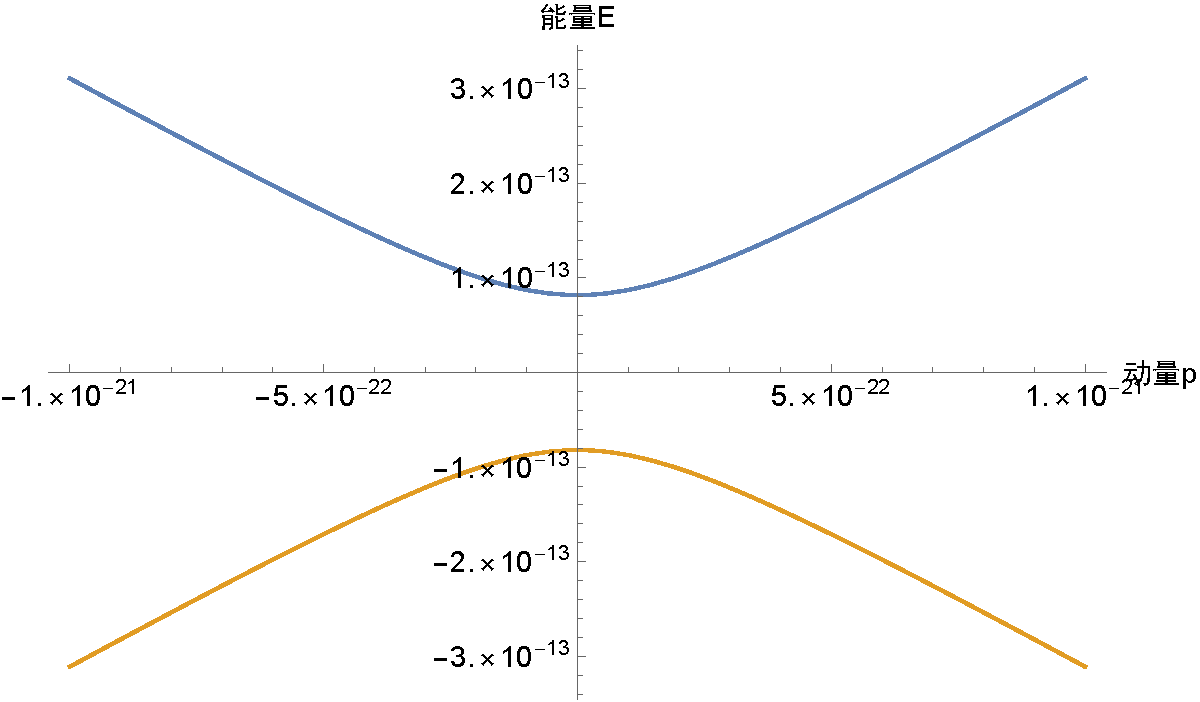
\includegraphics[width=5in]{dirac1.pdf}
  \caption{两种正负解的能谱图}\label{dirac pic 1}
\end{figure}
    狄拉克解释负能态是填满的,并且由于泡利不相容原理占据了各个状态。单粒子负能解是负能态海洋的空穴。狄拉克方程和薛定谔方程不同,狄拉克方程是多粒子方程,薛定谔方程是单粒子方程。\\
    在变换$m\rightarrow-m$和$\beta\rightarrow-\beta$下狄拉克方程保持不变。这表明粒子和反粒子是拓扑不可分辨的。

    最后补充一下关于Dirac表象和Weyl表象之间的关系
    对于狄拉克方程的$\alpha,\beta$和$\gamma$矩阵之间的关系
    \begin{equation}
        \alpha^i=\gamma^0\gamma^i,\quad \beta=\gamma^0
    \end{equation}
    对于狄拉克表象下,$\gamma$矩阵表示为
    \begin{equation}
        \gamma^0=\begin{bmatrix}
            I&0\\
            0&-I
        \end{bmatrix},\quad\gamma^k=\begin{bmatrix}
            0&\sigma^k\\
            -\sigma^k&0
        \end{bmatrix},\quad\gamma^5=i\gamma^0\gamma^1\gamma^2\gamma^3=\begin{bmatrix}
            0&I\\
            I&0
        \end{bmatrix}
    \end{equation}
    显然,在这个表象下,$\alpha^k,\beta$表示为
    \begin{equation}
        \alpha^k=\gamma^0\gamma^k=\begin{bmatrix}
            0&\sigma^k\\
            \sigma^k&0
        \end{bmatrix}=\sigma^1\otimes\sigma^k,\quad\beta=\gamma^0=\begin{bmatrix}
            I&0\\
            0&-I
        \end{bmatrix}=\sigma^3\otimes\sigma^0
    \end{equation}
    另一个我们常用的表象是Weyl表象
    \begin{equation}
        \gamma^0=\begin{bmatrix}
            0&I\\
            I&0
        \end{bmatrix},\quad\gamma^k=\begin{bmatrix}
            0&\sigma^k\\
            -\sigma^k&0
        \end{bmatrix},\quad\gamma^5=\begin{bmatrix}
            -I&0\\
            0&I
        \end{bmatrix}
    \end{equation}
    在这个表象下$\alpha^k,beta$表示为
    \begin{equation}
        \alpha^k=\gamma^0\gamma^k=\begin{bmatrix}
            -\sigma^k&0\\
            0&\sigma^k
        \end{bmatrix}=-\sigma^3\otimes\sigma^k,\quad\beta-\gamma^0=\begin{bmatrix}
            0&I\\
            I&0
        \end{bmatrix}=\sigma^1\otimes\sigma^0
    \end{equation}
    从Weyl表象变到Dirac表象下的变换矩阵为
    \begin{equation}
        U=\begin{bmatrix}
            I&I\\
            -I&I
        \end{bmatrix},\quad \gamma_D^0=U\gamma_W^0U^{-1},\quad\psi_D=U\psi_W
    \end{equation}
\subsection{束缚态解}
\subsubsection{Jackiw-Rebbi的一维解}
在正负质量的两个区域之间表面的束缚态解暗示了狄拉克方程和拓扑绝缘体之间的联系。我们考虑正负质量的狄拉克方程
\begin{equation}
    h(x)=-iv\hbar\partial_x\sigma_x+m(x)v^2\sigma_z
\end{equation}
\begin{equation}
    m(x)=\begin{cases}
        &-m_1\quad x<0\\
        &+m_2\quad x>0
    \end{cases}
\end{equation}
这里$m_1,m_2>0$。我们使用了有效速度替换光速$c$。
\begin{figure}[h]
    \centering
    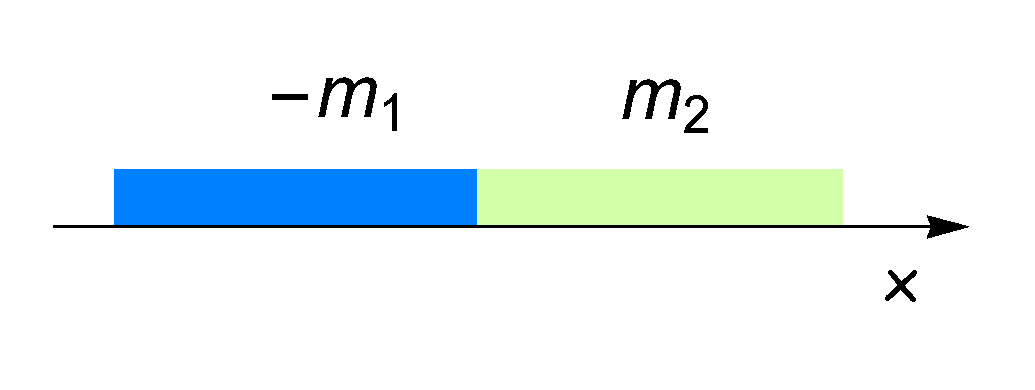
\includegraphics[width=3in]{dirac2.pdf}
    \caption{一维边界态}\label{dirac pic 2}
\end{figure}
狄拉克方程用于固体时,本征方程有形式
\begin{equation}
    \begin{bmatrix}
        m(x)v^2&-iv\hbar\partial_x\\
        -iv\hbar\partial_x&-m(x)v^2
    \end{bmatrix}\begin{bmatrix}
        \varphi_1(x)\\\varphi_2(x)
    \end{bmatrix}=E\begin{bmatrix}
        \varphi_1(x)\\\varphi_2(x)
    \end{bmatrix}
\end{equation}
对于两个区域$x>0,x<0$而言,方程是二阶常微分方程。我们可以分别单独求解。解必须在连接处$x=0$满足连续性。为了得到连接处附近的束缚态解,我们采用狄利克雷条件:波函数在$x=\pm\infty$处趋于$0$。\\
对于$x>0$我们有$m(x)=m_2$
\begin{equation}
    \begin{split}
        m_2v^2\psi_1^+(x)-iv\hbar\partial_x\psi_2^+(x)&=E\psi_1^+(x)\\
        -ib\hbar\partial_x\psi_1^+(x)-m_2v^2\psi_2^+(x)&=E\psi_2^+(x)
    \end{split}
\end{equation}
对第二式两边取$\partial_x$得到
\begin{equation}
    -iv\hbar\partial_x^2\psi_1^+(x)=(m_2v^2+E)\partial_x\psi_2^+(x)
\end{equation}
带入第一式得到
\begin{equation}
    v^2\hbar^2\partial_x^2\psi_1^+(x)=(m_2^2v^4-E^2)\psi_1^+(x)
\end{equation}
令$\lambda_+=\frac{\sqrt{m_2^2v^4-E^2}}{v\hbar}$得到
\begin{equation}
    \partial_x^2\psi_1^+(x)-\lambda_+^2\psi_1^+(x)=0
\end{equation}
解得:$\psi_1^+(x)=\psi_1^+e^{-\lambda_+x}$,边界条件$x\to+\infty,\psi_2^+(x)\to0$\\
利用$\partial_x\psi_2^+=\frac{m_2v^2-E}{iv\hbar}\psi_1^+(x)$得到
\begin{equation}
    \begin{split}
        \psi_2^+(x)&=\frac{-iv\hbar}{m_2v^2+E}\psi_1^+(-\lambda_+)e^{-\lambda_+x}\\
        &=i\frac{\sqrt{m_2^2v^4-E^2}}{m_2v^2+E}\psi_1^+e^{-\lambda_+x}\\
        &=i\sqrt{\frac{m_2v^2-E}{m_2v^2+E}}\psi_1^+e^{-\lambda_+x}
    \end{split}
\end{equation}
记$\psi_2^+(x)=\psi_2^+e^{-\lambda_+x}$
\begin{equation}
    \psi_2^+=i\sqrt{\frac{m_2v^2-E}{m_2v^2+E}}\psi_1^+
\end{equation}
\begin{equation}
    \psi_1^+=-i\sqrt{\frac{m_2v^2+E}{m_2v^2-E}}\psi_2^+=-\frac{iv\hbar\lambda_+}{m_2v^2-E}\psi_2^+
\end{equation}
对于$x<0$,$m(x)=-m_1$,我们有狄拉克方程
\begin{equation}
    \begin{split}
        -m_1v^2\psi_1^-(x)-iv\hbar\partial_x\psi_2^-(x)&=E\psi_1^-(x)\\
        -iv\hbar\partial_x\psi_1^-(x)+m_1v^2\psi_2^-(x)&=E\psi_2^-(x)
    \end{split}
\end{equation}
同样两边对第二式偏导得到
\begin{equation}
    v^2\hbar^2\partial_x^2\psi_1^-(x)-(m_1^2v^4-E^2)\psi_1^-(x)=0
\end{equation}
令$\lambda_-=\frac{\sqrt{m_1^2v^4-E^2}}{v\hbar}$
\begin{equation}
    \partial_x^2\psi_1^-(x)-\lambda_-^2\psi_1^-(x)=0
\end{equation}
得解为$\psi_1^-(x)=\psi_1^-e^{\lambda_-x}$,满足边界条件$x\to-\infty,\psi(x)\to0$\\
利用$\psi_2^-(x)=\frac{iv\hbar}{m_1v^2-E}\partial_x\psi_1^-(x)$得到
\begin{equation}
    \begin{split}
        \psi_2^-(x)&=\frac{iv\hbar}{m_1v^2-E}\psi_1^-\lambda_-e^{\lambda_-}x\\
        &=i\sqrt{\frac{m_1v^2+E}{m_1v^2-E}}\psi_1^-e^{\lambda_-x}
    \end{split}
\end{equation}
记$\psi_2^-(x)=\psi_2^-e^{\lambda_-x}$
\begin{equation}
    \psi_2^-=i\sqrt{\frac{m_1v^2+E}{m_1v^2-E}}\psi_1^-
\end{equation}
\begin{equation}
    \psi_1^-=-i\sqrt{\frac{m_1v^2-E}{m_1v^2+E}}\psi_2^-=-\frac{iv\hbar\lambda_-}{m_1v^2+E}\psi_2^-
\end{equation}
考虑连接处波函数连续,得到$\psi(0^-)=\psi(0^+)$
\begin{equation}
    \begin{bmatrix}
        \psi_1^+\\
        \psi_2^+
    \end{bmatrix}=\begin{bmatrix}
        \psi_1^-\\
        \psi_2^-
    \end{bmatrix}
\end{equation}
得到
\begin{equation}
    \frac{\lambda_+}{m_2v^2-E}=\frac{\lambda_-}{m_1v^2+E}\Rightarrow\sqrt{\frac{m_2v^2+E}{m_2v^2-E}}=\sqrt{\frac{m_1v^2-E}{m_1v^2+E}}
\end{equation}
显然存在一个$E=0$的特殊解,此时$\lambda_+=\frac{m_2v}{\hbar},\lambda_-=\frac{m_1v}{\hbar}$\\
有关系式:$\psi_2^+=i\psi_1^+,\psi_2^-=i\psi_1^-,\psi_1^+=\psi_1^-=C$
\begin{equation}
    \Psi(x)=C\begin{pmatrix}
        1\\
        i
    \end{pmatrix}e^{-\frac{m_2vx}{\hbar}},x>0\quad\Psi(x)=C\begin{pmatrix}
        1\\i
    \end{pmatrix}e^{\frac{m_1vx}{\hbar}},x<0
\end{equation}
归一化计算
\begin{equation}
    \begin{split}
        &\int_{-\infty}^{+\infty}|\Psi(x)|^*dx=1\\
        &\int_{-\infty}^{0}|C|^22e^{\frac{2m_1vx}{\hbar}}dx+\int_{0}^{+\infty}|C|^22e^{-\frac{2m_2vx}{\hbar}}dx=1\\
        &C=\sqrt{\frac{v}{\hbar}\frac{m_1m_2}{m_1+m_2}}
    \end{split}
\end{equation}
$E=0$对应的解为
\begin{equation}
    \Psi(x)\sqrt{\frac{v}{\hbar}\frac{m_1m_2}{m_1+m_2}}\begin{pmatrix}
        1\\i
    \end{pmatrix}e^{-\frac{|m(x)vx|}{\hbar}}
\end{equation}
这个解主要分布在表面或者domain wall附近,在远离原点以e指数形式衰减。波函数空间分布的特征长度为$\xi_{1,2}=\lambda_{\pm}^{-1}=\frac{\hbar}{|m_{1,2}v|}$。当$m_2\to+\infty$时,解依旧存在。在这种情况下对于$x>0,\Psi(x)\to0$。这里值得注意,波函数在表面处并不是0.我们认为真空作为一个无穷大正质量的系统,带有开边界条件的负质量系统在边界附近有一个束缚态。这个结果导致了一个对于边缘和表面态的一般图像。\\
\begin{figure}[h]
    \centering
    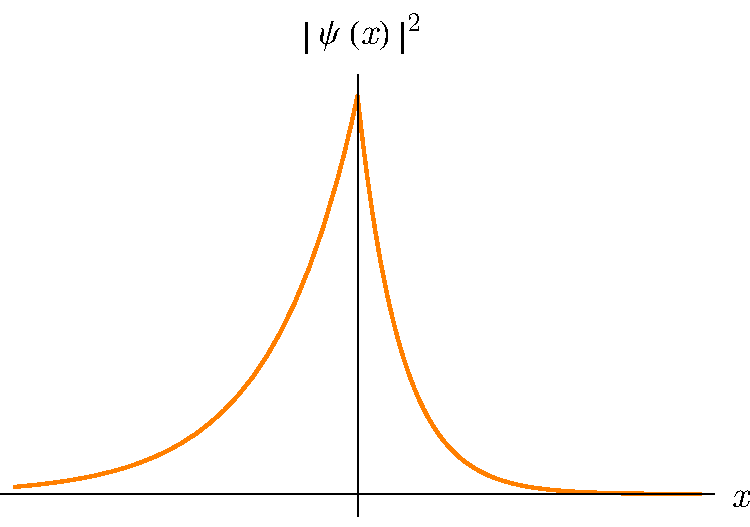
\includegraphics[width=2.5in]{dirac3.pdf}
    \caption{$-m_1<0$和$m_2>0$两个区域的波函数空间分布}\label{dirac pic 3}
  \end{figure}
对于质量分布连续,并且在两端异号的情况,我们可以找到一个一般形式的零能解。考虑$E=0$
\begin{equation}
    [-i\hbar\partial_x\sigma_x+m(x)v^2\sigma_z]\psi(x)=0
\end{equation}
两边同时乘以$\sigma_x$
\begin{equation}
    \partial_x\psi(x)=-\frac{m(x)v}{\hbar}\sigma_y\psi(x)
\end{equation}
进一步考虑$\sigma_y$的本征态
\begin{equation}
    \sigma_y\psi_\eta(x)=\eta\psi_\eta(x),\quad\psi_\eta(x)=\frac{1}{\sqrt{2}}\begin{pmatrix}1\\\eta i\end{pmatrix}\psi(x)
\end{equation}
把上面本征函数带入狄拉克方程得到
\begin{equation}
    \psi_\eta(x)\propto\frac{1}{\sqrt{2}}\begin{pmatrix}1\\\eta i\end{pmatrix}\exp\left[-\int^x\eta\frac{m(x')v}{\hbar}dx'\right]
\end{equation}
可以看出只要$m(+\infty)$和$m(-\infty)$异号,在domain wall处总是会存在零能解。因此,该解对质量分布$m(x)$具有很强的鲁棒性
\subsubsection{二维系统}
考虑一个二维系统,这里认为是$p_z=0$的三维系统。我们考虑沿着界面方向设为$y$轴。同样的,$x<0,-m_1<0,x>0,m2>0$。由于$y$方向平行,$p_y=\hbar k_y$是一个好量子数。我们可以利用一维解来求解二维解,首先是狄拉克方程哈密顿
\begin{equation}
    h(x)=-iv\hbar\partial_x\alpha_x-iv\hbar\partial_y\alpha_y+mv^2\beta
\end{equation}
这里$\alpha_x=\sigma_x\otimes\sigma_x,\alpha_y=\sigma_x\otimes\sigma_y,\beta=\sigma_z\otimes\sigma_0$.计算本征方程
\begin{equation}
    \left[(mv^2\sigma_z\otimes\sigma_0-iv\hbar\partial_x\sigma_x\otimes\sigma_x)-iv\hbar\partial_y\sigma_x\otimes\sigma_y\right]\Psi(x,k_y)=E\Psi(x,k_y)
\end{equation}
沿着$y$方向$p_y=\hbar k_y$是好量子数,所以令$\Psi(x,k_y)=\alpha_\eta\psi(x)e^{ik_yy}$是合理的本征函数,带入上式得到
\begin{equation}
    mv^2\sigma_z\otimes\sigma_0\alpha_\eta\psi(x)-iv\hbar(\sigma_x\otimes\sigma_x)\alpha_\eta\partial_x\psi(x)+v\hbar k_y(\sigma_x\otimes\sigma_y)\alpha_\eta\psi(x)=E\alpha_\eta\psi(x)
\end{equation}
简单化简一下得到
\begin{equation}
    mv^2(\sigma_z\otimes\sigma_0)\alpha_\eta\psi(x)-iv\hbar\partial_x\psi(x)(\sigma_x\otimes\sigma_x)\alpha_\eta=[E-v\hbar k_y(\sigma_x\otimes\sigma_y)\alpha_\eta]\psi(x)
\end{equation}
类比于x方向的一维系统,认为$\psi(x)=\sqrt{\frac{v}{\hbar}\frac{m_1m_2}{m_1+m_2}}e^{-\frac{|m(x)vx|}{\hbar}}$是合理的\\
带入上式,得到
\begin{equation}
    [mv^2(\sigma_x\otimes\sigma_0+i\sigma_x\otimes\sigma_x)]\alpha_\eta\psi(x)=[E-v\hbar k_y(\sigma_x\otimes\sigma_y)\alpha_\eta]\psi(x)
\end{equation}
现在求解矩阵$(\sigma_x\otimes\sigma_0+i\sigma_x\otimes\sigma_x)$与$\sigma_x\otimes\sigma_y$的本征值和本征向量
\begin{equation}
    \sigma_z\otimes\sigma_0+i\sigma_x\otimes\sigma_x=\begin{pmatrix}
        I&\quad\\\quad&-I
    \end{pmatrix}+i\begin{pmatrix}
        \quad&\sigma_x\\\sigma_x&\quad
    \end{pmatrix}=\begin{pmatrix}
        I&i\sigma_x\\i\sigma_x&-I
    \end{pmatrix}
\end{equation}
\begin{equation}
    \det\begin{pmatrix}
        \lambda-I&-i\sigma_x\\-i\sigma_x&\lambda-I
    \end{pmatrix}=0\quad\text{得到}\lambda=0
\end{equation}
令
\begin{equation}
    \alpha_\eta=\begin{pmatrix}
        \alpha\\\beta
    \end{pmatrix}
\end{equation}
带入上式得到
\begin{equation}
    \beta=i\sigma_x\alpha
\end{equation}
分别取$\alpha=(1,0)^T$和$(0,1)^T$得到的$\beta$分别为$(0,i)^T$和$(-i,0)^T$\\
所以对于矩阵$\sigma_z\otimes\sigma_0+i\sigma_x\otimes\sigma_x$只有一个零本征值,对应两个本征向量,分别为
\begin{equation}
    \alpha_\eta=\begin{pmatrix}
        1\\0\\0\\i
    \end{pmatrix}\text{或者}\begin{pmatrix}
        0\\1\\-i\\0
    \end{pmatrix}
\end{equation}
现在考虑$(\sigma_x\otimes\sigma_y)$的本征值和本征向量。
\begin{equation}
    \sigma_x\otimes\sigma_y=\begin{pmatrix}
        \quad&\sigma_y\\\sigma_y&\quad
    \end{pmatrix}\Rightarrow\lambda=\pm1
\end{equation}
$\lambda=1$时
\begin{equation}
    \begin{pmatrix}
        \quad&\sigma_y\\\sigma_y&\quad
    \end{pmatrix}\begin{pmatrix}
        \alpha\\\beta
    \end{pmatrix}=\begin{pmatrix}
        \alpha\\\beta
    \end{pmatrix}\Rightarrow\beta=\sigma_y\alpha
\end{equation}
同样的分别取$\alpha=(1,0)^T$和$(0,1)^T$得到$\beta$分别为$(0,i)^T$和$(-i,0)^T$\\
得到本征向量为
\begin{equation}
    \alpha_+=\begin{pmatrix}
        1\\0\\0\\i
    \end{pmatrix}\text{或者}\begin{pmatrix}
        0\\1\\-i\\0
    \end{pmatrix}
\end{equation}
$\lambda=-1$时
\begin{equation}
    \begin{pmatrix}
        \quad&\sigma_y\\\sigma_y&\quad
    \end{pmatrix}\begin{pmatrix}
    \alpha\\\beta
    \end{pmatrix}=-\begin{pmatrix}
        \alpha\\\beta
    \end{pmatrix}
\end{equation}
得到$\beta=-\sigma_y\alpha$,同样的分别取$\alpha=(1,0)^T$和$(0,1)^T$得到$\beta$分别为$(0,-i)$和$(i,0)^T$\\
所以本征向量为
\begin{equation}
    \alpha_-=\begin{pmatrix}
        1\\0\\0\\-i
    \end{pmatrix}\text{或}\begin{pmatrix}
        0\\1\\i\\0
    \end{pmatrix}
\end{equation}
综上考虑两个矩阵的共同本征向量得到
\begin{equation}
    \alpha_+=\begin{pmatrix}
        1\\0\\0\\i
    \end{pmatrix}\text{和}\alpha_-=\begin{pmatrix}
        0\\1\\i\\0
    \end{pmatrix}
\end{equation}
分别对应$\alpha_y$为$\pm1$的情况.\\
最后得到狄拉克方程的两个不同解
\begin{equation}
    \Psi_+(x,k_y)=\sqrt{\frac{v}{\hbar}\frac{m_1m_2}{m_1+m_2}}\begin{pmatrix}
        1\\0\\0\\i
    \end{pmatrix}e^{-\frac{|m(x)vx|}{\hbar}+ik_yy}
\end{equation}
能谱为$E_+(k)=v\hbar k_yy$
\begin{equation}
    \Psi_+(x,k_y)=\sqrt{\frac{v}{\hbar}\frac{m_1m_2}{m_1+m_2}}\begin{pmatrix}
        0\\1\\i\\0
    \end{pmatrix}e^{-\frac{|m(x)vx|}{\hbar}+ik_yy}
\end{equation}
能谱为$E_-(k)=-v\hbar k_yy$\\
根据两个本征态的能谱可以得到电子的有效速度$v_{\pm}=\frac{\partial E_{\pm}(k)}{\hbar k}=\pm v$.这说明每一个本征态都对应的有一个电流,沿着边界面,并且方向相反。电流密度在远离边界面指数衰减。当系统有时间反演对称性时,这两个态是时间反演对称的,构成一对手征边缘态。进一步说,$p_z=0$的狄拉克方程对于不同自旋能约化成两个独立的方程集
\begin{equation}
    h(x)=vp_x\sigma_x\pm vp_y\sigma_y+m(x)v^2\sigma_z
\end{equation}
两个束缚态速度反向就很明显了。

补充:
分块矩阵行列式计算公式
\begin{enumerate}
    \item 若$A$和$D$是方阵
    \begin{equation}
        \left|\begin{array}{ll}
            A & B \\
            0 & D
            \end{array}\right|=|A||D|
    \end{equation}
    \item
    \begin{equation}
        \text{若$A$可逆}\left|\begin{array}{ll}
            A & B \\
            C & D
            \end{array}\right|=|A|\left|D-C A^{-1} B\right|\quad\text{若$D$可逆}\left|\begin{array}{ll}
                A & B \\
                C & D
                \end{array}\right|=|D|\left|A-B D^{-1} C\right|
    \end{equation}
    \item 若$A,B,C,D$是同阶方阵,并且至少有一个是零矩阵则
    \begin{equation}
        \left|\begin{array}{ll}
            A & B \\
            C & D
            \end{array}\right|=|A D-B C|
    \end{equation}
    \item 若$A,B,C,D$是同阶方阵,则有如下四种情况
    \begin{equation}
    \begin{split}
        &\left|\begin{array}{ll}
            A & B \\
            C & D
            \end{array}\right|=|A D-C B|,(AC=CA),\quad\left|\begin{array}{ll}
                A & B \\
                C & D
                \end{array}\right|=|A D-B C|,(CD=DC),\quad \\
        &\left|\begin{array}{ll}
                    A & B \\
                    C & D
                    \end{array}\right|=|D A-B C|,(BD=DB),\quad \left|\begin{array}{ll}
                        A & B \\
                        C & D
                        \end{array}\right|=|D A-B C|,(AB=BA)
    \end{split}
    \end{equation}
    \item 若$A,B$是$n$阶方阵,则
    \begin{equation}
        \left|\begin{array}{ll}
            A & B \\
            B & A
            \end{array}\right|=|A+B||A-B|
    \end{equation}
\end{enumerate}
\subsubsection{三维和更高维}
在正负质量边界处总是存在束缚态。所有沿着表面其他分量的动量都是好量子数,在一维情况总是存在零模解。我们可以用解作为基去得到高维的非零模解。
\subsection{为何不是狄拉克方程}
从狄拉克方程里,我们知道在两个正负质量或者能隙的介质界面总是存在束缚态解。这些解对于界面的粗糙度或其他因素具有很强的robust。如果我们假设真空是一个绝缘体,具有无限大和正的质量或者能隙,那么这个带有负质量的系统在开边界周围存在束缚态解。这非常接近拓扑绝缘体的定义。然而由于狄拉克正负质量的对称性,在幺正变换后的两个系统是拓扑不可分的。我们并不能简单的从能隙或者质量符号上判断哪一个是拓扑平凡的哪一个是拓扑非平凡的。如果我们用狄拉克方程描述拓扑绝缘体,我们不得不引入额外的真空作为背景。这样我们认为额外条件是不需要的,因为束缚态的存在在拓扑绝缘体上应该有一个能带结构上物理和内蕴的结果。因此,我们推断狄拉克方程的本身用来描述拓扑量子材料可能不会是一个合适的方案。
\subsection{狄拉克方程的二次修正}
为了探索拓扑绝缘体可能的描述,我们在狄拉克方程的能隙或者说静止质量项中引入二次修正$-Bp^2$:
\begin{equation}
    H=vp\cdot\alpha+(mv^2-Bp^2)\beta
\end{equation}
其中$mv^2$是粒子的能隙,$m$和$v$分别有质量和速度的量纲。$B^{-1}$也有质量的量纲。二次项破坏了狄拉克方程中的$m\to-m$的对称性,让方程从原始的狄拉克方程变得拓扑可分辨。

为了解释这个,我们在动量空间中绘制了基态的动量分布,如图。在$p=0$处,自旋方向由$mv^2\beta$或者质量$m$的符号决定,但是对于$p$很大的情况,自旋方向则是由$-Bp^2\beta$或者说磁场$B$的符号决定。如果无量纲参数$mB>0$,当$p$沿着某个方向增加时(例如$x$方向),在$p^2_c=\frac{mv}{B}$处,自旋将会从$z$方向转到动量的$x$方向,在$p$足够大的时候,最终方向和$z$方向相反。这是由动量空间中的两个所谓的merons组成,它们被称为skymion。对于$mB<0$的情况,当$p$增加时,自旋将会从$z$方向旋转到动量方向,然后跳回原来$z$方向。在$p=0$或者$p=+\infty$处,自旋是否指向相同方向的特性决定了在$mB>0$和$mB<0$下的方程拓扑可分辨。
\subsection{修正狄拉克方程的束缚态解}
\subsection{一维:末端态}
我们从一维的情况开始,在这种情况下,$4\times4$的修正狄拉克方程可以解耦成两个独立的$2\times2$的狄拉克方程对于不同自旋能约化成两个独立的方程集
\begin{equation}
    h(x)=vp_x\sigma_x+(mv^2-Bp^2)\sigma_z
\end{equation}
对于半无穷长$x>0$的链,我们考虑$x=0$处的开边界条件。这要求了波函数在边界处为$0$,也就是所谓的狄利克雷条件。通常地,我们可以用一系列解来展开波函数延展到全空间的态。在这里我们只关心边界附近的束缚态解。为了找到零能解,我们有方程
\begin{equation}
    [vp_x\sigma_x+(mv^2-Bp_x^2)\sigma_z]\varphi(x)=0
\end{equation}
两边左乘$\sigma_x$得到
\begin{equation}
    \partial_x\varphi(x)=-\frac{1}{v\hbar}(mv^2+B\hbar^2\partial_x^2)\sigma_y\varphi(x)
\end{equation}
如果$\varphi(x)$是$\sigma_y$的本征函数,我们让$\varphi(x)=\chi_\eta\phi(x)$,其中$\sigma_y\chi_\eta=\eta\chi_\eta(\eta=\pm1)$. 那么微分方程约化成二阶常微分方程
\begin{equation}
    \partial_x\phi(x)=-\frac{\eta}{v\hbar}(mv^2+B\hbar^2\partial_x^2)\phi(x)
\end{equation}
设$\phi(x)=Ce^{-\lambda x}$得到久期方程
\begin{equation}
    B\hbar^2\lambda^2-\eta v\hbar\lambda+mv^2=0
\end{equation}
两个根满足韦达定理
\begin{equation}
    \lambda_++\lambda_-=\frac{\eta v}{\hbar B},\quad \lambda_+\lambda_-=\frac{mv^2}{B\hbar^2}
\end{equation}
我们要求波函数在$x=0$和$x=+\infty$处趋于$0$:
\begin{equation}
    \varphi(x=0)=\varphi(x=+\infty)=0
\end{equation}
不失一般性,我们认为有效速度$v>0$. 由于上面两个边界条件,我们必须要求久期方程的两个根是正的。这样$\chi_\eta$的本征值必须满足
\begin{equation}
    \begin{cases}
        \lambda_++\lambda_->0\\
        \lambda_+\lambda_->0
    \end{cases}\quad\Longrightarrow\begin{cases}
        \frac{\eta v}{\hbar B}>0\Longrightarrow\eta=\mathrm{sgn}(B)\\
        \frac{mv^2}{B\hbar^2}>0\Longrightarrow mB>0
    \end{cases}
\end{equation}
在这两个条件下,存在束缚态零能解
\begin{equation}
    \varphi_\eta(x)=\frac{C}{\sqrt{2}}\begin{pmatrix}
        \mathrm{sgn}(B)\\
        i
    \end{pmatrix}(e^{-\lambda_+x}-e^{-\lambda_-x})
\end{equation}
其中$\lambda_{\pm}=\frac{v}{2|B|\hbar}(1\pm\sqrt{1-4mB})$,$C$是归一化常数。这个解的主要性质是波函数主要分布在边界附近,在远离末端处指数衰减,如图所示。同样的我们令$\xi_\pm=\lambda_\pm^{-1}$,两个参数$\xi_->\xi_+$决定了波函数的空间分布,这是两个非常重要的特征长度,表示了末端态的特征。
\begin{equation}
    \text{当}B\to0\text{时}\Longrightarrow\begin{cases}
        \xi_+\to\frac{|B|\hbar}{v}\\
        \xi_-\to\frac{\hbar\mathrm{sgn}(B)}{mv}
    \end{cases}
\end{equation}
所以当$B\to0$时,$\xi_+$趋于$0$,而$\xi_-$趋于一个由能隙$mv^2$决定的有限值。如果我们放宽波函数在边界处的条件,在$B=0$时甚至也可以存在解。通过这种方式,我们回到了传统的狄拉克方程。在这种情况下,两个方程得到一个结果。当$m\to0$时,$\xi_-\to+\infty$,这表明末端态扩展到体态。这样,在$m=0$时末端态消失,发生拓扑量子相变。

\begin{figure}[h]
    \centering
    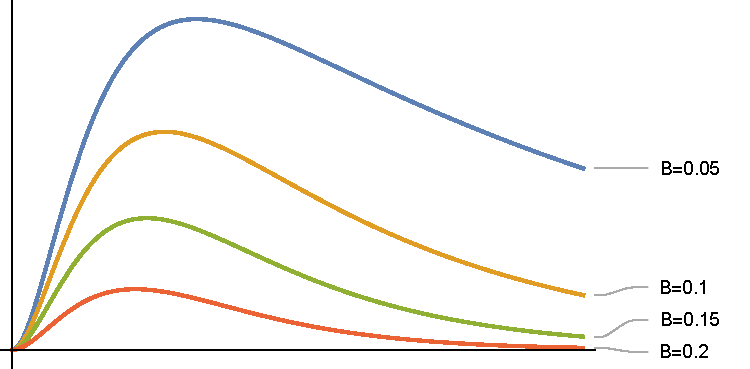
\includegraphics[width=2.5in]{dirac4.pdf}
    \caption{不同$B$对应修正狄拉克方程波函数空间分布}\label{dirac pic 4}
\end{figure}

在四分量形式,两个简并解有如下形式。
\begin{equation}
    \Psi_{1}=\frac{C}{\sqrt{2}}\left(\begin{array}{c}
        \operatorname{sgn}(B) \\
        0 \\
        0 \\
        i
        \end{array}\right)\left(e^{-x / \xi_{+}}-e^{-x / \xi_{-}}\right)
\end{equation}
\begin{equation}
    \Psi_{2}=\frac{C}{\sqrt{2}}\left(\begin{array}{c}
        0 \\
        s g n(B) \\
        i \\
        0
        \end{array}\right)\left(e^{-x / \xi_{+}}-e^{-x / \xi_{-}}\right)
\end{equation}
求解过程如下
\begin{equation}
    h(x)=vp_x\alpha_x+(mv^2-Bp^2)\beta
\end{equation}
求解零能解只需要让$h(x)\varphi(x)=0$
\begin{equation}
    -iv\hbar\alpha_x\partial_x\varphi(x)+(mv^2+B^2\hbar\partial_x^2)\beta\varphi(x)=0
\end{equation}
同样的做法,两边左乘$\alpha_x$得到
\begin{equation}
    \partial_x\varphi(x)=-\frac{1}{v\hbar}(mv^2+B\hbar^2\partial_x^2)(\sigma_y\otimes\sigma_x)\varphi(x)
\end{equation}
令$\varphi(x)=\chi_\eta\phi(x)$,其中$\chi_\eta$是$\sigma_y\otimes\sigma_x$的本征向量。
\begin{equation}
    \sigma_y\otimes\sigma_x=\begin{bmatrix}
        \quad&-i\sigma_x\\
        i\sigma_x&\quad
    \end{bmatrix}
\end{equation}
久期方程
\begin{equation}
    \left|\begin{matrix}
        \lambda I&i\sigma_x\\
        -i\sigma_x&\lambda I
    \end{matrix}\right|=0\Longrightarrow\lambda=\pm1
\end{equation}
假设狄拉克二旋量为$\chi_\eta=\begin{bmatrix}
    \alpha\\
    \beta
\end{bmatrix}$,满足
\begin{equation}
    (\sigma_y\otimes\sigma_x)\chi_\eta=\eta\chi_\eta
\end{equation}
这样就得到
\begin{equation}
    -i\sigma_x\beta=\alpha\Longrightarrow i\sigma_x\alpha=\eta\beta
\end{equation}
令$\alpha=\begin{bmatrix}
    \eta\\
    0
\end{bmatrix}$带入上式得到
\begin{equation}
    i\sigma_x\begin{bmatrix}
        \eta\\
        0
    \end{bmatrix}=i\begin{bmatrix}
        0\\
        \eta
    \end{bmatrix}=\eta\begin{bmatrix}
        0\\
        i
    \end{bmatrix}\Longrightarrow\beta=\begin{bmatrix}
        0\\
        i
    \end{bmatrix}\Longrightarrow\chi_\eta=\begin{bmatrix}
        \eta\\
        0\\
        0\\
        i
    \end{bmatrix}
\end{equation}
令$\alpha=\begin{bmatrix}
    0\\
    \eta
\end{bmatrix}$带入上式得到
\begin{equation}
    i\sigma_x\begin{bmatrix}
        0\\
        \eta
    \end{bmatrix}=i\begin{bmatrix}
        \eta\\
        0
    \end{bmatrix}=\eta\begin{bmatrix}
        i\\
        0
    \end{bmatrix}\Longrightarrow\beta=\begin{bmatrix}
        i\\
        0
    \end{bmatrix}\Longrightarrow\chi_\eta=\begin{bmatrix}
        0\\
        \eta\\
        i\\
        0
    \end{bmatrix}
\end{equation}
所以把$\varphi(x)=\chi_\eta\phi(x)$带入修正狄拉克方程得到
\begin{equation}
    \partial_x\phi(x)=-\frac{\eta}{v\hbar}(mv^2+B\hbar^2\partial_x^2)\phi(x)
\end{equation}
该方程与边界条件与之前二分量一维end态一样,照抄过来得到四分量一维end态
\begin{equation}
    \psi_{1}=\frac{C}{\sqrt{2}}\left(\begin{array}{c}
        \operatorname{sgn}(B) \\
        0 \\
        0 \\
        i
        \end{array}\right)\left(e^{-x / \xi_{+}}-e^{-x / \xi_{-}}\right)
\end{equation}
\begin{equation}
    \Psi_{2}=\frac{C}{\sqrt{2}}\left(\begin{array}{c}
        0 \\
        \operatorname{sgn}(B) \\
        i \\
        0
        \end{array}\right)\left(e^{-x / \xi_{+}}-e^{-x / \xi-}\right)
\end{equation}
我们将会看到这两个方程是求解高维有效哈密顿解的基础。

该解在拓扑绝缘子理论中的作用不可低估。我们将会看到所有的边缘态或表面态的解,以及拓扑激发都与这个解密切相关。
\subsubsection{二维:手征边缘态}
在二维的情况下,方程可以解耦成两个独立方程
\begin{equation}
    h_\pm=vp_x\pm vp_y\sigma_y+(mv^2-Bp^2)\sigma_z
\end{equation}
这两个方程破坏了时间反演对称$\sigma_i\rightarrow-\sigma_i,p_i\rightarrow-p_i$

我们考虑半无穷长的平面,$x=0$处有狄利克雷条件。$p_y=\hbar k_y$是一个好量子数。在$k_y=0$处,二维方程有和一维四分量形式一样的解。$x$方向的解有和一维一样的解。这样我们用两个一维解$\{\Psi_1,\Psi_2\}$作为基底。$y$的独立部分$H_{2D}=vp_y\alpha_y-Bp_y^2\beta$可以被视为一维哈密顿的微扰。这样我们有了一维边缘态的有效模型
\begin{equation}
    H_{eff}=\begin{pmatrix}
        \langle\Psi_1|\Delta H_{2D}|\Psi_1\rangle&\langle\Psi_1|\Delta H_{2D}|\Psi_2\rangle\\
        \langle\Psi_2|\Delta H_{2D}|\Psi_1\rangle&\langle\Psi_2|\Delta H_{2D}|\Psi_2\rangle
    \end{pmatrix}=vp_y\mathrm{sgn}(B)\sigma_z
\end{equation}
证明:我们已知
\begin{equation}
    \begin{split}
        |\Psi_1\rangle&=\chi_\eta^1\phi(x)\\
        |\Psi_2\rangle&=\chi_\eta^2\phi(x)
    \end{split}
\end{equation}
计算矩阵元
\begin{equation}
    \begin{split}
        \langle\Psi_i|\Delta H_{2D}|\Psi_j\rangle&=\int dx(\chi_\eta^i)^\dagger\phi^*(x)(vp_y\alpha_y-Bp_y^2\beta)\chi_\eta^j\phi(x)\\
        &=(\chi_\eta^i)^\dagger(vp_y\alpha_y-Bp_y^2\beta)\chi_\eta^j
    \end{split}
\end{equation}
分别计算$(\chi_\eta^i)^\dagger\alpha_y\chi_\eta^j$和$(\chi_\eta^i)^\dagger\beta\chi_\eta^j$得到
\begin{equation}
    H_{eff}=vp_y\mathrm{sgn}(B)\sigma_z
\end{equation}
$B$的符号函数表明了一个事实,当$B=0$时手征边缘态消失。束缚态色散关系为
\begin{equation}
    \epsilon_{p_y,\pm}=\pm vp_y
\end{equation}
电子分别在两个不同的态里有正负速度$(\pm v)$,构成一对手征边缘态。

二维情况的边缘态精确解有类似于一维情况的形式
\begin{equation}
    \psi_{1}=\frac{C}{\sqrt{2}}\left(\begin{array}{c}
        \mathrm{sgn}(B) \\
        0 \\
        0 \\
        i
        \end{array}\right)\left(e^{-x / \xi_{+}}-e^{-x / \xi_{-}}\right) e^{+i p_{y} y / \hbar}
\end{equation}
\begin{equation}
    \psi_{2}=\frac{C}{\sqrt{2}}\left(\begin{array}{c}
        0 \\
        \mathrm{sgn}(B) \\
        i \\
        0
        \end{array}\right)\left(e^{-x / \xi_{+}}-e^{-x / \xi_{-}}\right) e^{+i p_{y} y / \hbar}
\end{equation}
分别对应两个不同的色散关系$\epsilon_{p_y\pm}=\pm vp_y\mathrm{sgn}(B)$. 特征长度依赖于$p_y$
\begin{equation}
    \xi_{\pm}^{-1}=\frac{v}{2|B|\hbar}\left(1\pm\sqrt{1-4mB+\frac{4B^2p_y^2}{v^2}}\right)
\end{equation}
在二维情况TKNN整数可以用来表示系统是否拓扑非平凡。对于两带哈密顿形式$H=d(p)\cdot\sigma$,Chern数可以表示成
\begin{equation}
    n_{c}=-\frac{1}{4 \pi} \int d \mathbf{p} \frac{\mathbf{d} \cdot\left(\partial_{p_{x}} \mathbf{d} \times \partial_{p_{y}} \mathbf{d}\right)}{d^{3}}
\end{equation}
其中$d^2=\sum_{\alpha}d_\alpha^2$. 积分跑遍整个第一布里渊区,Chern数$n_c$总是整数。在连续极限下,积分区域变得无穷大,积分可以出现分数。对于上述哈密顿,Chern数计算出来的结果为
\begin{equation}
    n_{\pm}=\pm(\mathrm{sgn}(m)+\mathrm{sgn}(B))/2
\end{equation}
这与霍尔电导率有关$\sigma_\pm=n_\pm e^2/h$,当$m$和$B$有相同符号时候,$n_\pm=\pm1$,这个时候是拓扑非平凡的,当$m,B$有不同符号时,$n_\pm=0$,这个时候是拓扑平凡的。拓扑非平凡条件与边缘态条件$mB>0$一致。这表示了量子整数霍尔效应的体边对应。
\subsubsection{三维情况:表面态}
在三维情况下,我们考虑$x=0$处的$y-z$平面。我们可以根据一维束缚态解推导出表面的有效模型。因为$y-z$平面的动量是好量子数,我们用他们的本征值替代动量算符$p_y,p_z$。考虑$p_y-$和$p_z-$分量作为一维哈密顿$H_{1D}$的微扰:
\begin{equation}
    \Delta H_{3D}=vp_y\alpha_y+v_z\alpha_z-B(p_y^2+p_z^2)\beta
\end{equation}
$p_y=p_z=0$处的三维狄拉克方程的解和一维解$|\Psi_1\rangle,|\Psi_2\rangle$有一样的形式。对于$p_y,p_z\neq0$,我们用解
\begin{equation}
    \psi_{1}=\frac{C}{\sqrt{2}}\left(\begin{array}{c}
        \operatorname{sgn}(B) \\
        0 \\
        0 \\
        i
        \end{array}\right)\left(e^{-x / \xi_{+}}-e^{-x / \xi_{-}}\right) e^{i\left(p_{y} y+p_{z} z\right) / \hbar}
\end{equation}
\begin{equation}
    \psi_{2}=\frac{C}{\sqrt{2}}\left(\begin{array}{c}
        0 \\
        \operatorname{sgn}(B) \\
        i \\
        0
        \end{array}\right)\left(e^{-x / \xi_{+}}-e^{-x / \xi_{-}}\right) e^{i\left(p_{y} y+p_{z} z\right) / \hbar}
\end{equation}
作为一组基底。利用微扰有效哈密顿可以算出
\begin{equation}
    H_{e f f}=\left(\begin{array}{cc}
        \left\langle\Psi_{1}\left|\Delta H_{2 D}\right| \Psi_{1}\right\rangle & \left\langle\Psi_{1}\left|\Delta H_{2 D}\right| \Psi_{2}\right\rangle \\
        \left\langle\Psi_{2}\left|\Delta H_{2 D}\right| \Psi_{1}\right\rangle & \left\langle\Psi_{2}\left|\Delta H_{2 D}\right| \Psi_{2}\right\rangle
        \end{array}\right)=v\mathrm{sgn}(B)(p\times\sigma)_x
\end{equation}
计算过程和之前一样。做一个幺正变换
\begin{equation}
    \begin{aligned}
        &\Phi_{1}=\frac{1}{\sqrt{2}}\left(\left|\Psi_{1}\right\rangle-i\left|\psi_{2}\right\rangle\right)\\
        &\Phi_{2}=\frac{-i}{\sqrt{2}}\left(\left|\Psi_{1}\right\rangle+i\left|\Psi_{2}\right\rangle\right)
    \end{aligned}
\end{equation}
得到无能隙的狄拉克方程表面态
\begin{equation}
    \begin{aligned}
H_{e f f} &=\frac{1}{2}\left(\left\langle\Phi_{1}\left|,\left\langle\Phi_{2}\right|\right) \Delta H_{3 D}\left(\begin{array}{c}
\left|\Phi_{1}\right\rangle \\
\left|\Phi_{2}\right\rangle
\end{array}\right)\right.\right.\\
&=\operatorname{vsgn}(B)\left(p_{y} \sigma_{y}+p_{z} \sigma_{z}\right)
\end{aligned}
\end{equation}
\begin{figure}[h]
    \centering
    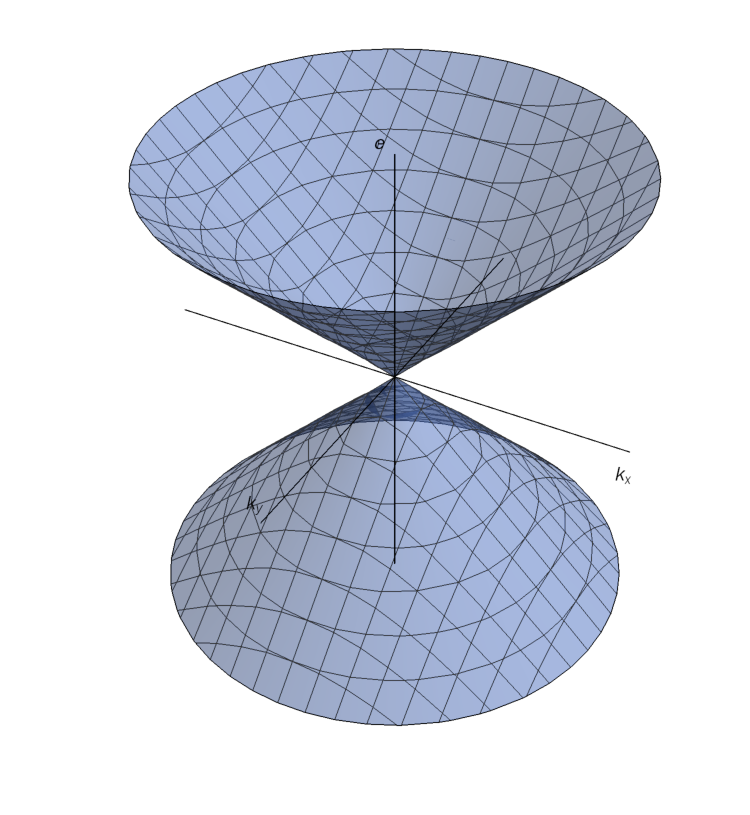
\includegraphics[width=2in]{dirac5.pdf}
    \caption{\footnotesize{三维表面态色散关系}}\label{dirac pic 5}
\end{figure}

色散关系为$\epsilon_\pm=\pm vp,p=\sqrt{p_x^2+p_y^2}$. 利用这种方式,我们对于表面态的狄拉克锥有了一个有效模型,如图所示。值得注意$\sigma_i$在哈密顿里不是真实的自旋,是$p_y=p_z=0$处两个态决定的。在一些系统里$|\Psi_1\rangle,|\Psi_2\rangle$几乎沿$z$方向的电子自旋极化。在这个情况里泡利矩阵可以被视为真实自旋的一种近似。

三维表面态的精确求解为
\begin{equation}
    \Psi_{\pm}=C \Psi_{\pm}^{0}\left(e^{-x / \xi_{+}}-e^{-x / \xi_{-}}\right) \exp \left[+i\left(p_{y} y+p_{z} z\right) / \hbar\right]
\end{equation}
其中
\begin{equation}
    \Psi_{+}^{0}=\left(\begin{array}{c}
        \cos \frac{\theta}{2} \operatorname{sgn}(B) \\
        -i \sin \frac{\theta}{2} \operatorname{sgn}(B) \\
        \sin \frac{\theta}{2} \\
        i \cos \frac{\theta}{2}
        \end{array}\right)\quad \Psi_{-}^{0}=\left(\begin{array}{c}
            \sin \frac{\theta}{2} \operatorname{sgn}(B) \\
            i \cos \frac{\theta}{2} \operatorname{sgn}(B) \\
            -\cos \frac{\theta}{2} \\
            i \sin \frac{\theta}{2}
            \end{array}\right)
\end{equation}
色散关系为$\epsilon_{p,\pm}=\pm v\mathrm{sgn}(B)$,$\tan \theta=p_y/p_z$,特征深度$\xi_{\pm}$变成依赖于$p$的量。
\begin{equation}
    \xi_{\pm}^{-1}=\frac{v}{2|B| \hbar}(1 \pm \sqrt{1-4 m B+4 B^{2} p^{2} / \hbar^{2}})
\end{equation}
\section{拓扑绝缘体的最小晶格模型}
\subsection{紧束缚近似}
紧束缚模型广泛应用于描述固体电子的能带。下图的示意图从原子物理学的角度描述了紧束缚晶格的形成。考虑一个孤立原子,比如氢原子。在量子力学里,电子围绕原子核在库伦势下运动,形成一系列分立的能级或者说轨道,$E_n=-\frac{e^2}{8\pi\epsilon_0n^2a)0}$,其中$a_0$是波尔半径,$n$是整数能级序数。基态能是$E_{n=1}=-13.6eV$,半径为$a_0=0.529$\AA. 第一激发态的能量为$E_{n=2}=-3.4eV$. 这两个态之间的能量差为$-10.2eV$. 这在固体中是非常大的。所以在低温下认为只有基态电子是一个很好的近似。当两个原子靠得很近时,不同原子的两个电子轨道可能在空间中产生交叠。一个原子的电子有可能调到另一个原子的轨道上去。因为电子主要局域化在原子核周围,电子从一个原子隧穿到另一个原子的轨道上的概率依旧很小。这个图像可以推广到由原子构成的晶格系统:电子从一个原子跃迁到另一个原子形成能带。

在二次量子化表象下,哈密顿的有效模型可以写成
\begin{equation}
    H=\sum_{i,\sigma=\uparrow\downarrow}\epsilon_0c_{i,\sigma}^\dagger-\sum_{\langle i,j\rangle,\sigma=\uparrow,\downarrow}t_{ij}c_{i,\sigma}^\dagger c_{j,\sigma}
\end{equation}
期指那个对$i$求和跑遍真个晶格位点,$\sigma=\uparrow,\downarrow$表示电子自旋向上和向下。$c_{i,sigma}^\dagger,c_{i\sigma}$是电子在位点$i$自旋向上或者向下的产生湮灭算符,分别服从反对易关系$\{c_{i,\sigma},c_{j,\sigma'}^\dagger\}=\delta_{i,j}\delta_{\sigma,\sigma'}$. 湮灭算符要求$c_{i,\sigma}|0\rangle=0$表示电子从位点$i$隧穿到$j$的隧穿振幅。

对于$N$格点的一维周期晶格,我们有$c_{i,\sigma}=c_{i+N,\sigma}$. 为了简单起见,我们假设晶格具有平移不变性,所以$t_{ij}=t$。利用傅里叶变换得到
\begin{equation}
    c_{i,\sigma}=\frac{1}{\sqrt{Na}}\sum_{k_n}e^{ik_n R_i}c_{k_n,\sigma}
\end{equation}
\begin{equation}
    c_{i,\sigma}^\dagger=\frac{1}{\sqrt{Na}}\sum_{k_n}e^{-ik_n R_i}c_{k_n,\sigma}^\dagger
\end{equation}
周期性条件给出$e^{ik_nR_i}=e^{ik_n(R_i+Na)}\Rightarrow k_n=\frac{2\pi n}{Na}(n=0,\pm1,\pm2,\cdots,N-1)$. 用这种方式,哈密顿可以对角化为
\begin{equation}
    \begin{split}
        H&=\sum_{i,\sigma}\epsilon_0c_{i\sigma}c_{i\sigma}-\sum_{\langle i,j\rangle,\sigma}t_{ij}c_{i\sigma}c_{j\sigma}\\
        &=\sum_{i,\sigma}\frac{\epsilon_0}{Na}\sum_{k_n,k_n'}e^{-i(k_n'-k_n)R_i}c_{k_n'\sigma}^\dagger c_{k_n\sigma}-\sum_{\langle i,j\rangle,\sigma}\frac{t}{Na}\sum_{k_n,k_n'}e^{-i(k_n'R_i-k_nR_j)}c_{k_n',\sigma}^\dagger c_{k_n,\sigma}\\
        &=\sum_{k_n,\sigma}\epsilon_0c_{k_n\sigma}^\dagger c_{k_n\sigma}-\frac{t}{Na}\sum_{i\rho\sigma}\sum_{k_n,k_n'}e^{-i(k_n'-k_n)R_i}e^{ik_n\rho a}c_{k_n'\sigma}^\dagger c_{k_n\sigma}\\
        &=\sum_{k_n\sigma}(\epsilon_0-2t\cos k_n a)c_{k_n\sigma}^\dagger c_{k_n\sigma}=\sum_{k_n,\sigma}\epsilon(k_n)c_{k_n\sigma}^\dagger c_{k_n\sigma}
    \end{split}
\end{equation}
所以我们看到在紧束缚近似中考虑最近邻相互作用的色散关系为$\epsilon(k_n)=\epsilon_0-2t\cos k_na$. 值得注意$K=\frac{2\pi}{a},\epsilon(k_n+K)=\epsilon(k_n)$. 对于比较大的$N$,$k_n$可以连续的从$0$取到$\frac{2\pi}{a}$,$K$被叫做倒格子的格矢。

该方法可以推广到二维和三维。倒格矢可以定义为从实空间到动量空间的傅里叶变换。在三维晶格中的晶格基矢设为$a,b,c$,倒格矢被定义为
\begin{equation}
    K_a=2\pi\frac{b\times c}{a\cdot(b\times c)},\quad K_b=2\pi\frac{c\times a}{a\cdot(b\times c)},\quad K_c=2\pi\frac{a\times b}{a\cdot(b\times c)},\quad K_i\cdot R_j=2\pi\delta_{ij}
\end{equation}
\subsection*{关于紧束缚近似}
\subsubsection*{平移算符}
因为电子在固体中感受到的晶格势是位置的周期函数,引入晶格平移算符是很有必要的
\begin{equation}
    Tf(x)=f(x+a)
\end{equation}
其中$f(x)$是位置的任意函数,$a$是晶格周期。显然$T$与单粒子哈密顿对易
\begin{equation}
    H=-\frac{\hbar^2}{2m}\frac{\partial^2}{\partial x^2}+V(x)
\end{equation}
这很显然,因为我们设$x'=x+a$,很显然$\frac{\partial}{\partial x'}=\frac{\partial}{\partial x}$,$V(x')=V(x)$.

线性代数告诉我们,如果两个线性算符相互对易,那么对于他们存在共同的本征函数。我们假设$\Psi$是$H$和$T$的共同本征态。
\begin{equation}
    H\Psi=E\Psi,\quad T\Psi=\lambda\Psi
\end{equation}
其中$E,\lambda$是本征值。显然,把$T$作用$N$次
\begin{equation}
    T^N\Psi(x)=\lambda^N\Psi(x)=\Psi(x+Na)
\end{equation}
我们采用周期性边界条件,所以有$\Psi(x+Na)=\Psi(x)$,这意味着
\begin{equation}
    T^N\Psi(x)=\Psi(x)\Longrightarrow\lambda^N=1\Longrightarrow\lambda=e^{i\frac{2\pi n}{N}}
\end{equation}
其中$n=0,\pm1,\pm2\cdots$. 我们也可以写成
\begin{equation}
    \lambda=e^{ika}
\end{equation}
其中$k=\frac{2\pi n}{Na}$. 显然相差$\frac{2\pi}{a}$的两个不同的$k$给出同一个$\lambda$. 和通常一样,对于一维晶格我们在$-\pi/a<k<\pi/a$的范围内选择$N$个独立的$k$,这正好是一维晶格的第一布里渊区。

对于一维以上的系统,$T_R$表示平移一个晶格矢量
\begin{equation}
    T_R\Psi(r)=e^{ik\cdot R}\Psi(r)
\end{equation}
其中$k=\frac{n_1}{N_1}b_1+\frac{n_2}{N_2}b_2+\frac{n_3}{N_3}b_3$,这里$n_1,n_2,n_3$是整数,$b_1,b_2,b_3$是倒格子的基矢量。我们对于周期边界$L_1=N_1a,L_2=N_2a,L_3=N_3a$有一个周期表姐条件,$n_1,n_2,n_3$的取值将$k$约束在了第一布里渊区。
\subsubsection*{布洛赫定理}
刚才解释一维$N$原子晶格和周期性边界条件
\begin{equation}
    T\Psi(x)=\Psi(x+a)=e^{ika}\Psi(x)
\end{equation}
其中在第一布里渊区有$N$个独立的$k$。我们可以定义函数
\begin{equation}
    u_k(x)=e^{-ikx}\Psi(x)
\end{equation}
显然
\begin{equation}
    Tu_k(x)=T\{e^{ikx}\Psi(x)\}=e^{-ik(x+a)}\Psi(x+a)=e^{-ikx}\Psi(x)=u_k(x)
\end{equation}
因此,我们得到布洛赫函数
\begin{equation}
    \Psi(x)=e^{ikx}u_k(x)
\end{equation}
$u_k(x)$是一个周期函数$u_k(x+a)=u_k(x)$. 这就是众所周知的Bloch定理。
\subsubsection*{紧束缚近似/LCAO}
我们假设自由原子有势场$V_a(r)$,以至于传导电子(例如钠原子$3s$上的电子)满足薛定谔方程
\begin{equation}
    \left(-\frac{\hbar^{2}}{2 m} \nabla^{2}+V_{a}(r)-E_{a}\right) \phi(r)=0
\end{equation}
这里$E_a$表示传导电子的单原子能级。当原子形成晶格时,原子之间的独立势相互交叠,如图所示
\begin{figure}[h]
    \centering
    
\includegraphics[width=6in]{dirac6.pdf}
    \caption{\footnotesize{单原子势和晶格势比较}}\label{dirac pic 6}
\end{figure}
在紧束缚近似中,我们假设原胞$R_j$中的电子受到其他不在$R_j$的原子的影响是很微小的。它在原胞$R_j$中的波函数应该很接近单原子能级$E_a$的波函数$\phi(r-R_j)$. 我们可以对原子轨道波函数$\phi(r-R_j)$线性组合来作为固体电子中的试探波函数。

为了满足Bloch定理,我们如下构造
\begin{equation}
    \Psi_{k}(r)=\frac{1}{\sqrt{N}} \sum_{j} \mathrm{e}^{\mathrm{i} \mathbf{k} \cdot \mathbf{R}_{j}} \phi\left(r-R_{j}\right)
\end{equation}
显然平移算符作用在$\Psi_k$得到
\begin{equation}
    \begin{split}
        T_{R_n}\Psi_k(r)&=\Psi_k(r+R_n)=\frac{1}{\sqrt{N}}\sum_{j}e^{ik\cdot R_j}\phi(r-R_j+R_n)\\
        &=\mathrm{e}^{\mathrm{i} \mathbf{k} \cdot \mathbf{R}_{n}} \frac{1}{\sqrt{N}} \sum_{j} \mathrm{e}^{\mathrm{i} \mathbf{k} \cdot\left(\mathbf{R}_{j}-\mathbf{R}_{n}\right)} \phi\left(r-R_{j}+R_{n}\right)=\mathrm{e}^{\mathrm{i} \mathbf{k} \cdot \mathbf{R}_{n}} \Psi_{k}(r)
    \end{split}
\end{equation}
$\Psi_k$态的能量由下式给出
\begin{equation}
    E_k=\frac{\langle \Psi_k|H|\Psi_k\rangle}{\langle\Psi_k|\Psi_k\rangle}
\end{equation}
其中哈密顿是电子在晶格里的哈密顿,此外还有
\begin{equation}
    \langle\Psi_k|\Psi_k\rangle=\frac{1}{N}\sum_{j,m}e^{ik\cdot(R_j-R_m)}\int d^3r\phi^*(r-R_m)\phi^*(r-R_j)
\end{equation}
如果忽略$\phi(r-R_j)$和$\phi(r-R_m)$的交叠,$d^3r$的积分给出的是$\delta_{j,m}$,对$j$求和得到是晶格总数$N$.

对于固体中的电子哈密顿所包含的势$V(r)$. 我们也可以写成
\begin{equation}
    V(r)=V_a(r-R_j)+\tilde{V}(r-R_j)
\end{equation}
换句话说,$\tilde{V}(r-R_j)$是固体的全体势减去局域在$R_j$原子的势。从图表中可以看出$V_a$比$V(r)$要大,所以$\tilde{V}(r-R_j)$是负的。
对于局域在$R_j$的单原子哈密顿有
\begin{equation}
    \left[-\frac{\hbar^{2}}{2 m} \nabla^{2}+V_{a}\left(r-R_{j}\right)-E_{a}\right] \phi\left(r-R_{j}\right)=0
\end{equation}
所以$\Psi_k$对应的能级能量为
\begin{equation}
    E_k=\langle\Psi_k|H|\Psi_k\rangle=\frac{1}{N} \sum_{j} \sum_{m} \mathrm{e}^{\mathrm{i} \mathbf{k} \cdot\left(R_{j}-R_{m}\right)} \int \mathrm{d}^{3} r \phi^{*}\left(r-R_{m}\right)\left[E_{a}+\tilde{V}\left(r-R_{j}\right)\right] \phi\left(r-R_{j}\right)
\end{equation}
第一项$E_a$是单原子能级的能量,是个常数,并且能拿出积分外。由于$|\Psi_k\rangle$的归一化条件,第一项拿出积分后得到的数值就是$E_a$. 然后我们定义下列数值
\begin{equation}
    \begin{aligned}
        &\alpha=-\int \mathrm{d}^{3} r \phi^{*}\left(r-R_{j}\right) \tilde{V}\left(r-R_{j}\right) \phi\left(r-R_{j}\right)\\
        &\gamma=-\int \mathrm{d}^{3} r \phi^{*}\left(r-R_{m}\right) \tilde{V}\left(r-R_{j}\right) \phi\left(r-R_{j}\right)
    \end{aligned}
\end{equation}
由于平移对称性,$\alpha,\gamma$是一个与格点指标无关的常数。考虑最近邻相互作用,我们得到
\begin{equation}
    E_k=E_a-\alpha-\gamma\sum_{\langle j,m\rangle}'e^{ik\cdot(R_j-R_m)}
\end{equation}
我们选择减号的原因是因为$\tilde{V}(r-R_j)$本身就是负的,这样选择可以使$\alpha,\gamma$为正。

我们举一个三维方晶格的例子
\begin{equation}
    E_k=E_a-\alpha-2\gamma(\cos k_xa+\cos k_ya+\cos k_za)
\end{equation}
由于$\gamma,\alpha>0$
\begin{equation}
    E_k^{Min}=E_a-\alpha-6\gamma,\quad E_k^{Max}=E_a-\alpha+6\gamma
\end{equation}
\begin{center}
\begin{tikzpicture}[domain=-pi:pi]
    \draw[->,thick] (-6,0) -- (6,0)node[right]{$k$\;[1,1,1]};
    \draw[->,thick] (0,-0.5) --(0,2.5)node[above]{$E_k$};
    \draw[color=orange,very thick] plot (\x,{1-cos(\x r)});
    \node[below=0.7em,right] (0,0) {$E_a-\alpha-6\gamma$};
    \draw[dashed,color=red] (pi,0)node[below]{$\frac{\pi}{a}$} -- (pi,2.5)node[below=0.8em,right]{$E_a-\alpha+6\gamma$};
    \draw[dashed,color=red] (-pi,0)node[below]{$-\frac{\pi}{a}$} -- (-pi,2.5)node[below=0.8em,left]{$E_a-\alpha+6\gamma$};
    \node[right] at (0,1) {$E_a-\alpha$};
    \node[right] at (0,1.4) {$E_a$};
    \draw (-0.1,1) -- (0.1,1);
    \draw (-0.1,1.4) -- (0.1,1.4);
    \node[color=blue][rotate = 90] at (3.4,1) {$\underbrace{\hspace{2cm}}$};
    \node at (3.5,1) {能带宽度$\Delta E=12\gamma$};
\end{tikzpicture}\\
\footnotesize{方晶格紧束缚近似的色散关系}
\end{center}
对于长波极限$k\ll\frac{\pi}{a}$泰勒展开得到
\begin{equation}
    \begin{aligned}
        E_{k} & \simeq E_{a}-\alpha-6 \gamma+\gamma a^{2} k^{2} ; \quad k^{2}=k_{x}^{2}+k_{y}^{2}+k_{z}^{2} \\
        &=E_{k}^{\operatorname{Min}}+\frac{\hbar^{2} k^{2}}{2 m^{*}}
        \end{aligned}
\end{equation}
有效质量$m^*=\frac{\hbar^2}{2\gamma a^2}$. 当$\gamma$减小时,能带宽度$\Delta E$也随之减小,$E=E_k^{Min}$附近的有效质量增加。下面是二维方晶格色散关系:
\begin{figure}[h]
    \centering
    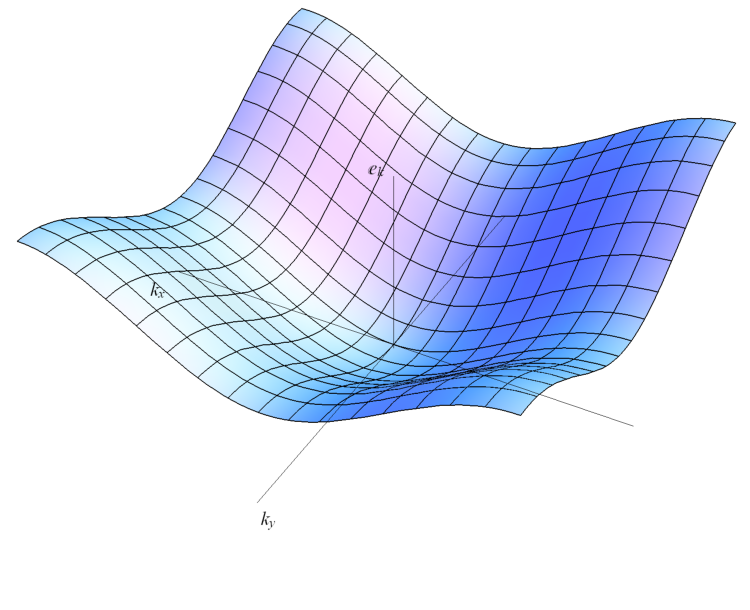
\includegraphics[width=2in]{dirac7.pdf}
    \caption{\footnotesize{二维方晶格色散关系}}\label{dirac pic 7}
\end{figure}
\subsubsection*{紧束缚近似二次量子化}
假设自由电子系统由哈密顿
\begin{equation}
    H_{0}=\sum_{k} \varepsilon_{k} c_{k}^{\dagger} c_{k}
\end{equation}
描述,其中$\varepsilon_k=\frac{\hbar k^2}{2m}$是动能项。在周期势场里$V(r)=\sum_{K}V_{K}e^{iK\cdot r}$,我们能写出二次量子化形式
\begin{equation}
    H^{\prime}=\sum_{k, K} V_{K} c_{k+K}^{\dagger} c_{k}
\end{equation}
现在引入格点$R_n^0$上的产生湮灭算符$c_n,c_n^\dagger$
\begin{equation}
    c_n=\frac{1}{\sqrt{N}}\sum_{k}c_ke^{ik\cdot R_n^0}
\end{equation}
逆变换为
\begin{equation}
    c_{k}=\frac{1}{\sqrt{N}} \sum_{n} c_{n} \mathrm{e}^{-\mathrm{i} \mathbf{k} \cdot \mathbf{R}_{n}^{0}}
\end{equation}
带入动能项$H_0$中得到
\begin{equation}
    H_0=\sum_{k}\varepsilon_k\sum_{n,m}\frac{1}{N}c_n^\dagger c_m e^{ik\cdot(R_n^0-R_m^0)}
\end{equation}
定义
\begin{equation}
    T_{n m}=\frac{1}{N} \sum_{k} \varepsilon_{k} \mathrm{e}^{\mathrm{ik} \cdot\left(\mathbf{R}_{n}^{0}-\mathbf{R}_{m}^{0}\right)}
\end{equation}
得到
\begin{equation}
    H_{0}=\sum_{n m} T_{n m} c_{n}^{\dagger} c_{m}
\end{equation}
现在计算$H'$
\begin{equation}
    \begin{aligned}
        H^{\prime} &=\sum_{\mathbf{k}, \mathbf{K}} V_{K} \frac{1}{N} \sum_{n m} c_{n}^{\dagger} \mathrm{e}^{\mathrm{i}(\mathbf{k}+\mathbf{K}) \cdot \mathbf{R}_{n}^{0}} c_{m} \mathrm{e}^{-\mathrm{i} \mathbf{k} \cdot \mathbf{R}_{m}^{0}} \\
        &=\sum_{\mathbf{K} n m}\left[\sum_{k} \frac{1}{N} \mathrm{e}^{\mathrm{i} \mathbf{k} \cdot\left(\mathbf{R}_{n}^{0}-\mathbf{R}_{m}^{0}\right)}\right] V_{K} \mathrm{e}^{\mathrm{i} \mathbf{K} \cdot \mathbf{R}_{n}^{0}} c_{n}^{\dagger} c_{m}
        \end{aligned}
\end{equation}
由于$\frac{1}{N} \sum_{k} \mathrm{e}^{\mathrm{i} \mathbf{k} \cdot\left(\mathbf{R}_{n}^{0}-\mathbf{R}_{m}^{0}\right)}=\delta_{n m}$, 我们有
\begin{equation}
    H^{\prime}=\sum_{\mathbf{K}, n} V_{K} \mathrm{e}^{\mathrm{i} \mathrm{K} \cdot \mathbf{R}_{n}^{0}} c_{n}^{\dagger} c_{n}
\end{equation}
我们记$\sum_K V_K e^{i\mathbf{K}\cdot\mathbf{R}_n^0}=V(\mathbf{R}_n^0)$
\begin{equation}
    H^{\prime}=\sum_{n} V\left(R_{n}^{0}\right) c_{n}^{\dagger} c_{n}
\end{equation}
考虑$H_0$后得到
\begin{equation}
    \begin{aligned}
        H &=\sum_{n}\left(T_{n n}+V\left(R_{n}^{0}\right)\right) c_{n}^{\dagger} c_{n}+\sum_{n \neq m} T_{n m} c_{n}^{\dagger} c_{m} \\
        &=\sum_{n} \varepsilon_{n} c_{n}^{\dagger} c_{n}+\sum_{n \neq m} T_{n m} c_{n}^{\dagger} c_{m}
        \end{aligned}
\end{equation}
其中$\epsilon_n=T_{nn}+V(R_n^0)$表示在位点$n$的能量,$T_{nm}$表示从位点$n$隧穿到$m$的振幅。从原子能级开始,允许能带中的近邻格点隧穿,能带宽度依赖于隧穿振幅$T_nm$
\subsection{从连续到晶格系统}
连续模型通常描述长波长度极限下的低能物理。能带结构的拓扑应能反映出布里渊区整个能带结构的性质。实际上,人们喜欢用晶格模型而不是连续模型去探索系统的拓扑。一个连续模型可以在紧束缚模型下映射到一个晶格模型,其中布里渊区是有限的。

通常地从一个连续系统映射到格点系统常用的方法是晶格离散化,例如一维晶格链
\begin{center}
    \begin{tikzpicture}
        \draw[->] (0,-1) -- (1,-1)node[right]{$x$};
        \fill (-2,0) circle (0.1);
        \fill (-1,0) circle (0.1);
        \fill (0,0) circle (0.1);
        \fill (1,0) circle (0.1);
        \fill (2,0) circle (0.1);
        \node at (3,0) {$\cdots$};
        \node at (-3,0) {$\cdots$};
        \node at (-3,1) {$j=$};
        \node at (-2,1) {$-2$};
        \node at (-1,1) {$-1$};
        \node at (0,1) {$0$};
        \node at (1,1) {$1$};
        \node at (2,1) {$2$};
        \node at (3,1) {$3$};
    \end{tikzpicture}
\end{center}
在格点中的坐标$x=ja$是离散的数,我们计算一维狄拉克方程在格点$x=ja$的离散条件
\begin{equation}
    \left[h(x)\psi(x)\right]_{x=ja}=\left.-iv\hbar\alpha_x\partial_x\psi(x)\right|_{x=ja}+(mv^2+B\hbar^2\partial_x^2)\beta\psi(x)
\end{equation}
一般而言求解狄拉克方程时我们将狄拉克波函数分解成旋量部分和函数部分$\psi(x)=\chi_\eta\phi(x)$. $\chi_\eta$是$\alpha,\beta$的本征列向量。这样我们实际上只需要考虑关于$\phi$的二阶微分方程求解。我们定义
\begin{equation}
    \phi_j\rightarrow\phi(x=ja)
\end{equation}
我们现在用导数的有限差分近似。假设晶格常数$a$很小,我们可以把一阶导数近似为
\begin{equation}
    \left[\frac{\mathrm{d}\phi}{\mathrm{d}x}\right]_{x=(j+\frac{1}{2})a}\rightarrow\frac{1}{a}[\phi_{j+1}-\phi_{j}]
\end{equation}
同样的,二阶导数可以计算出来
\begin{equation}
    \begin{split}
        \left[\frac{\mathrm{d}^2\phi}{\mathrm{d}x^2}\right]_{x=ja}&\rightarrow\frac{1}{a}\left\{\left[\frac{\mathrm{d}\phi}{\mathrm{d}x}\right]_{x=(j+\frac{1}{2})a}-\left[\frac{\mathrm{d}\phi}{\mathrm{d}x}\right]_{x=(j-\frac{1}{2})a}\right\}\\
        &\rightarrow\frac{1}{a}\left(\frac{1}{a}\left(\phi_{j+1}-\phi_{j}\right)-\frac{1}{a}(\phi_j-\phi_{j-1})\right)\\
        &\rightarrow\frac{1}{a^2}(\phi_{j+1}-2\phi_{j}+\phi_{j+1})
    \end{split}
\end{equation}
对于$h(x)$而言$\psi(x)=\chi_\eta\phi(x),\phi(x)=e^{ikx}$是一个本征函数。在离散晶格下,对应的差分方程为
\begin{equation}
    [h(x)\psi(x)]_{j}=-iv\hbar\alpha_x\frac{1}{2a}(\psi_{j+1}-\psi_{j-1})+mv^2\beta\psi_j+B\hbar^2\beta\frac{1}{a^2}(\psi_{j+1}-2\psi_{j}+\psi_{j-1})
\end{equation}
其中$\psi_j=\chi_\eta\phi_j$. 我们带入本征函数$\psi_j=\chi_\eta e^{ikja}$得到
\begin{equation}
    \begin{split}
        h(x)\psi(x)|_{x=ja}&=[v\hbar\alpha_x\chi_\eta\frac{1}{a}\sin ka+mv^2\beta\chi_\eta+\frac{B\hbar^2}{a^2}(2\cos ka-2)\beta\chi_\eta]\phi_j\\
        &=[v\hbar\alpha_x\frac{1}{a}\sin ka+(mv^2-\frac{2B\hbar^2}{a^2}(1-\cos ka))\beta]\psi_j
    \end{split}
\end{equation}
与一维连续系统狄拉克方程比较,我们得到一维替换
\begin{equation}
    \begin{split}
        &k_x\rightarrow\frac{1}{a}\sin k_xa\\
        &k_x^2\rightarrow\frac{2}{a^2}(1-\cos k_xa)
    \end{split}
\end{equation}
推广到$d$维超立方晶格中,有替换
\begin{equation}
    \begin{split}
        &k_i\rightarrow \frac{1}{a}\sin k_i a\\
        &k_i^2\rightarrow\frac{4}{a^2}\sin^2\frac{k_i a}{2}=\frac{2}{a^2}(1-\cos k_ia)
    \end{split}
\end{equation}
其中只在长波极限下成立,也就是说$k_ia\to0$时利用关系式$sin\sim x$. 对于$k_i^2$,我们用$\sin^2\frac{k_ia}{2}$或者$\cos k_ia$而不是$\sin^2k_ia$,这是为了避免有效哈密顿里长距离隧穿。通过这种方式,晶格模型中的隧穿项仅仅在最近邻之间存在。

通常在晶格模型中对于无质量狄拉克粒子存在倍增问题。替换$k_i\to\frac{\sim k_ia}{a}$对于$k_ia=\pi$处会引起额外的零点。这样在方晶格里对于无带隙的狄拉克方程会存在四个狄拉克锥。分别是$k=(0,0),k=(0,\frac{\pi}{a}),(\frac{\pi}{a},0),(\frac{\pi}{a},\frac{\pi}{a})$. 因为$\frac{4B}{a^2}\sin^2\frac{k_ia}{2}\to Bk^2$,足够大的$B$会消除掉在$(\frac{\pi}{a},\frac{\pi}{a})$的零点。这样,晶格模型在$B$足够大的条件下等价于连续模型。\textcolor[rgb]{1,0,0}{对于有限的$B$,在晶格模型中,由于$k_i$的线性项和二次项相互竞争,能带在$\Gamma$点可能不会打开}\footnote{这块目前我也没搞明白,希望有懂的可以交流一下。暂时不去思考,我们继续往前走。}。这个事实可能导致从大$B$连续变化到小$B$的一个拓扑相变。类似的相变也在高维系统中存在。因此,当我们研究紧束缚近似中的连续模型时,应该小心。然而,如果当模型参数连续变化时,能带中的能隙没有关闭然后打开,能带的拓扑结构就绝不会发生改变。

利用这个映射,我们得到拓扑绝缘体的晶格模型
\begin{equation}
    H=\frac{\hbar v}{a}\sum_{i=x,y,z}\sin k_ia\alpha_i+\left(mv^2-B\frac{4\hbar^2}{a^2}\sum_{i=x,y,z}\sin^2\frac{k_ia}{2}\right)\beta
\end{equation}
系统的能谱为
\begin{equation}
    E_{k,\pm}=\pm \sqrt{\frac{\hbar^{2} v^{2}}{a^{2}} \sum_{i=x, y, z} \sin ^{2} k_{i} a+\left(m v^{2}-\frac{4 B \hbar^{2}}{a^{2}} \sum_{i=x, y, z} \sin ^{2} \frac{k_{i} a}{2}\right)^{2}}
\end{equation}
对于$mB<0$,两个能带之间存在能隙$2|m|v^2$. 对于$mB=0,b\neq0$,能隙在$k_ia=0$处闭合,闭合点$E_{0+}=E_{0-}$. 对于$mB>0$,存在一系列无带隙点,对于一二三维系统$mv^2=\frac{4B\hbar^2}{a^2}$处,对于二三维系统$mv^2=\frac{8B\hbar^2}{a^2}$处,对于三维系统$mv^2=\frac{12B\hbar^2}{a^2}$处。我们会看到,对于量子相变这些正好是相变点。为了简化,我们设$a=\hbar=1$.

\begin{figure}[h]
    \centering
    \begin{minipage}[c]{0.3\textwidth}
        \centering
        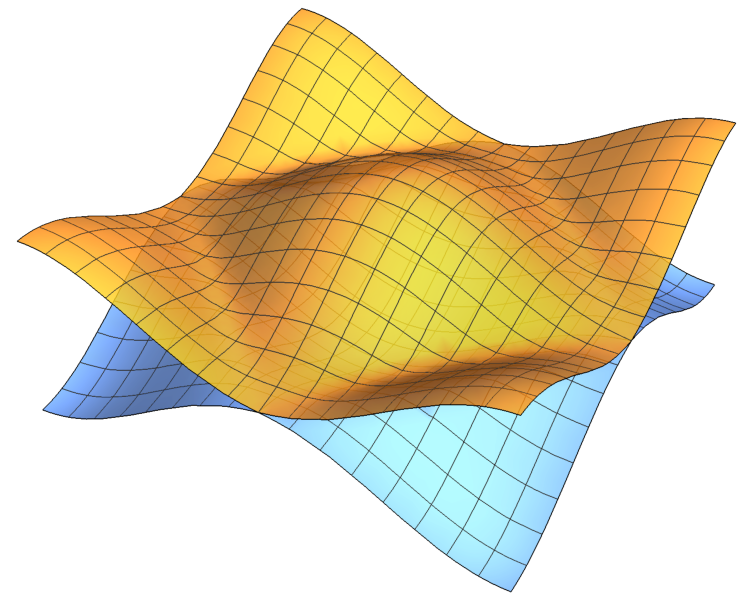
\includegraphics[width=1.5in]{dirac8m4.pdf}
        \caption{$mv^2=\frac{4B\hbar^2}{a^2}$}
    \end{minipage}
    \begin{minipage}[c]{0.3\textwidth}
        \centering
        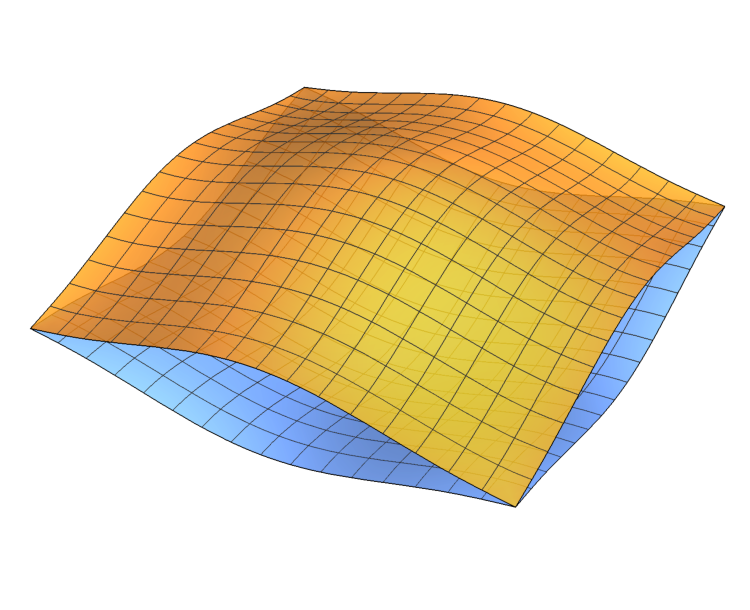
\includegraphics[width=1.5in]{dirac8m8.pdf}
        \caption{$mv^2=\frac{8B\hbar^2}{a^2}$}
    \end{minipage}
    \begin{minipage}[c]{0.3\textwidth}
        \centering
        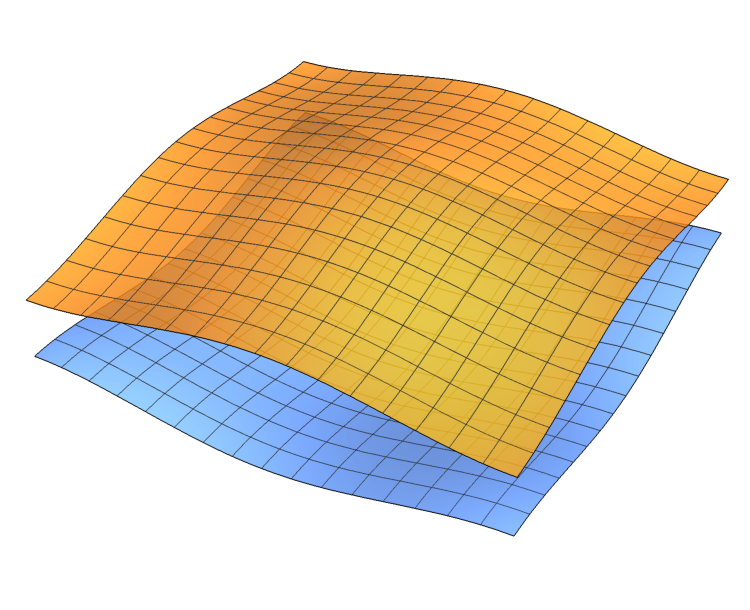
\includegraphics[width=1.5in]{dirac8m12.pdf}
        \caption{$mv^2=\frac{12B\hbar^2}{a^2}$}
    \end{minipage}
\end{figure}
我们可以做一个傅里叶变换,将有效哈密顿从动量空间变到格点空间。在紧束缚近似下,超立方晶格中的哈密顿有如下形式
\begin{equation}
    \begin{aligned}
        H=& \sum_{i, n, m} \Delta c_{i, n}^{\dagger} \beta_{n m} c_{i, m}-t \sum_{\langle i, j\rangle,n,m} c_{j, n}^{\dagger} \beta_{n m} c_{i m}+i t^{\prime} \sum_{i,a, n, m}\left[c_{i+a, n}^{\dagger}\left(\alpha_{a}\right)_{n m} c_{i m}-c_{i, n}^{\dagger}\left(\alpha_{a}\right)_{n m} c_{i+a, m}\right]
    \end{aligned}
\end{equation}
二次量子化的过程很简单。在$k$空间里二次量子化哈密顿写成
\begin{equation}
    H=\frac{\hbar v}{a}\sum_{a}\sum_{k_a}\sin k_aa\sum_{m,n}c_{\vec{k},n}^\dagger(\alpha_a)_{nm}c_{\vec{k},m}+\sum_{\vec{k}}\sum_{m,n}mv^2c_{\vec{k},n}\beta_{nm}c_{\vec{k},m}-\frac{4B\hbar^2}{a^2}\sum_{a}\sum_{k_a}\sum_{m,n}\sin^2 \frac{k_aa}{2}c_{\vec{k},n}^\dagger\beta_{nm}c_{\vec{k},m}
\end{equation}
带入傅里叶变换
\begin{equation}
    \begin{split}
        c_{\vec{k}}&=\frac{1}{\sqrt{Na}}\sum_{i}e^{-i\vec{k}\cdot\vec{R}_i}c_i\\
        c_{\vec{k}}^\dagger&=\frac{1}{\sqrt{Na}}\sum_{i}e^{i\vec{k}\cdot\vec{R}_i}c_i^\dagger
    \end{split}
\end{equation}
利用$\sin k_aa=\frac{1}{2i}(\exp(ik_a)-\exp(-ika))$. 上式第一项我们得到
\begin{equation}
    \begin{split}
        term 1&=\frac{\hbar v}{a}\sum_{a}\sum_{k_a,m,n}\frac{1}{2i}(e^{ik_aa}-e^{-ik_aa})\frac{1}{Na}\sum_{i,j}e^{i\vec{k}\cdot(\vec{R}_j-\vec{R}_i)}c_{j,n}^\dagger(\alpha_a)_{nm}c_{i,m}\\
        &=-i\frac{\hbar v}{2a}\sum_{a}\sum_{m,n,i,j}[\delta_{j+a,i}c_{j,n}^\dagger(\alpha_a)_{nm}c_{i,m}-\delta_{j,i+a}c_{j,n}^\dagger(\alpha_a)_{nm}c_{i,m}]\\
        &=i\frac{\hbar v}{2a}\sum_{i,a,n,m}[c_{i+a,n}^\dagger(\alpha_a)_{nm}c_{i,m}-c_{i,n}^\dagger(\alpha_a)_{nm}c_{i+a,m}]
    \end{split}
\end{equation}
对于第二项
\begin{equation}
    \begin{split}
        term2&=mv^2\sum_{\vec{k},m,n}c_{\vec{k},n}^\dagger\beta_{nm}c_{\vec{k},m}\\
        &=\frac{mv^2}{Na}\sum_{\vec{k},m,n}\sum_{i,j}e^{-i\vec{k}\cdot(\vec{R}_j-\vec{R}_{i})}c_{j,n}^\dagger\beta_{nm}c_{i,m}\\
        &=mv^2\sum_{i,m,n}c_{i,n}^\dagger\beta_{nm}c_{i,m}
    \end{split}
\end{equation}
对于\textbf{\textcolor[rgb]{1,0,0}{第三项}}\footnote{第三项的第一项不知道为什么计算上少了一个$d$,我暂时也没想明白哪里算错了,先不管了,往前走}
\begin{equation}
    \begin{split}
        term3&=-\frac{4B\hbar^2}{a^2}\sum_{a}\sum_{k_a}\sum_{m,n}\sin^2\frac{k_aa}{2}c_{\vec{k},n}^\dagger\beta_{nm}c_{\vec{k},m}\\
        &=-\frac{2B\hbar^2}{a^2}\sum_{a}\sum_{k_a}\sum_{m,n}(1-\cos k_aa)c_{\vec{k},n}^\dagger\beta_{nm}c_{\vec{k},m}\\
        &=-\frac{2dB\hbar^2}{a^2}\sum_{i,m,n}c_{i,n}^\dagger\beta_{nm}c_{i,m}+\frac{2B\hbar^2}{a^2}\sum_{a,k_a,m,n}\cos k_aac_{\vec{k},n}^\dagger\beta_{nm}c_{\vec{k},m}
    \end{split}
\end{equation}
利用欧拉公式$\cos x=\frac{1}{2i}(\exp(ix)+\exp(-ix))$
我们得到
\begin{equation}
    \begin{split}
        term3&=-\frac{2dB\hbar^2}{a^2}\sum_{i,m,n}c_{i,n}^\dagger\beta_{nm}c_{i,m}+\frac{2B\hbar^2}{a^2}\sum_{i,n,m}[c_{i+a,n}^\dagger\beta_{nm}c_{i,m}+c_{i,n}^\dagger\beta_{nm}c_{i+a,m}]\\
        &=-\frac{2dB\hbar^2}{a^2}\sum_{i,m,n}c_{i,n}^\dagger\beta_{nm}c_{i,m}+\frac{2B\hbar^2}{a^2}\sum_{n,m,\langle i,j\rangle}c_{j,n}^\dagger\beta_{nm}c_{i,m}
    \end{split}
\end{equation}
把这三项加起来就是上述格点表象中的哈密顿形式,
\begin{equation}
    \begin{split}
        H=\sum_{i,n,m}(mv^2-d\frac{2B\hbar^2}{a^2})c_{i,n}^\dagger\beta_{nm}c_{i,m}+\frac{2B\hbar^2}{a^2}\sum_{n,m,\langle i,j\rangle}c_{j,n}^\dagger\beta_{nm}c_{i,m}+i\frac{\hbar v}{2a}\sum_{i,a,n,m}[c_{i+a,n}^\dagger(\alpha_a)_{nm}c_{i,m}-c_{i,n}^\dagger(\alpha_a)_{nm}c_{i+a,m}]
    \end{split}
\end{equation}
其中$\langle i,j\rangle$跑遍所有的最近邻格点,$a=x,y,z$,$i+a$代表晶格坐标$R_i+R_a$. $n,m=1,2,\cdots,d$,$d$表示狄拉克矩阵的维数。比较参数可以知道系数为
\begin{equation}
    t'=\frac{\hbar v}{2a},\quad \Delta=mv^2+2dt,\quad t=-\frac{B\hbar^2}{a^2}
\end{equation}
用$c_i^\dagger$标记$(c_{i,1}^\dagger,c_{i,2}^\dagger,\cdots,c_{i,d}^\dagger)$. 通过这种方式,方程可以写成紧凑的形式
\begin{equation}
    H=\sum_{i}\Delta c_{i}^\dagger\beta c_{i}-t\sum_{\langle i,j\rangle}c_{j}^\dagger\beta c_{i}+it'\sum_{i,a}[c_{i+a}^\dagger\alpha_a c_i-c_i^\dagger\alpha_a c_{i+a}]
\end{equation}
\subsection{一维晶格}
考虑一个一维晶格模型
\begin{equation}
    H=\Delta\sum_{j=1}^{N}c_j^\dagger\sigma_zc_j-t\sum_{j=1}^{N-1}(c_{j+1}^\dagger\sigma_zc_j+c_j^\dagger\sigma_zc_{j+1})+it'\sum_{i=1}^{N-1}(c_{j+1}^\dagger\sigma_xc_j-c_j^\dagger\sigma_xc_{j+1})
\end{equation}
其中$c_j^\dagger=(c_{j,\uparrow}^\dagger,c_{j,\downarrow}^\dagger)$. 为了寻找到末端态,我们采用开边界条件。我们选择$(c_1^\dagger,c_2^\dagger,\cdots,c_N^\dagger)$作为基底。哈密顿可以写成矩阵的形式
\begin{equation}
    H=\left(\begin{array}{cccccc}
        \Delta \sigma_{z} & T & 0 & 0 & \ldots & 0 \\
        T^{\dagger} & \Delta \sigma_{z} & T & 0 & \ldots & 0 \\
        0 & T^{\dagger} & \Delta \sigma_{z} & T & \ldots & 0 \\
        \vdots & \vdots & \ddots & \ddots & \ddots & \vdots \\
        0 & 0 & 0 & T^{\dagger} & \Delta \sigma_{z} & T \\
        0 & 0 & 0 & 0 & T^{\dagger} & \Delta \sigma_{z}
        \end{array}\right)
\end{equation}
其中$T=-t\sigma_z-it'\sigma_x$. 因为$\sigma_x,\sigma_z$都是$2\times 2$的矩阵,哈密顿是$2N\times2N$的矩阵。我们知道泡利矩阵的关系为
这里我们给出半无穷长末端在$j=1,N=+\infty$的解。我们令$\Psi^\dagger=(\Psi_1^\dagger,\Psi_2^\dagger,\cdots,\Psi_N^\dagger)$为$H$的本征向量。本征方程变成
\begin{equation}
    \Delta\sigma_z\Psi_j+T\Psi_{j+1}+T^\dagger\Psi_{j-1}=E\Psi_j
\end{equation}
其中$j=1,2,\cdots$以及$\Psi_0=0$. 为了求解这个方程,我们带入试探解
\begin{equation}
    \Psi_{j+1}=\lambda\Psi_{j}=\lambda^{j+1}\Psi
\end{equation}
这样本征方程变成
\begin{equation}
    (\Delta\sigma_z+\lambda T+\lambda^{-1}T^\dagger)\Psi=P\Psi=E\Psi
\end{equation}
其中,算符$P=\Delta\sigma_z+\lambda T+\lambda^{-1}T^\dagger=\gamma\cdot\sigma$
\begin{equation}
    \begin{split}
        \gamma_x&=-it'(\lambda-\lambda^{-1})\sigma_x\\
        \gamma_y&=0\\
        \gamma_z&=\Delta-\lambda t-\lambda^{-1}t
    \end{split}
\end{equation}
一般而言,矩阵$P$是一个非厄米矩阵,对于一个$P$可能有两个复本征值。但是对于实际物理系统的本征值,$E$必须是实数。所以$P$不得不至少满足下列两个条件之一
\begin{enumerate}
    \item $\gamma$所有的分量都是实的.
    \item 所有非$0$复分量的组合给出$E=0$.
\end{enumerate}
当$\lambda=e^{ik}$时,第一个条件显然满足,这给出体带的解。这个在这里不是我们所关系的解。第二个条件定义了所谓的零化子,在这个条件下,$P$的本征值对应的$E=0$. 所以我们有
\begin{equation}
    P=\gamma\cdot\sigma=\gamma_x\sigma_x+\gamma_z\sigma_z=\begin{bmatrix}
        \gamma_z&\gamma_x\\
        \gamma_x&-\gamma_z
    \end{bmatrix},\quad(\gamma_y=0)
\end{equation}
对应的久期方程为
\begin{equation}
    \left|\begin{matrix}
        E-\gamma_z&-\gamma_x\\
        -\gamma_x&E+\gamma_z
    \end{matrix}\right|=0\Longrightarrow E=\pm\sqrt{\gamma_x^2+\gamma_z^2}=0
\end{equation}
也就是说$\gamma_x^2+\gamma_z^2=0$. 对该式子做标准分解得到
\begin{equation}
    (\gamma_x+i\gamma_z)(\gamma_x-i\gamma_z)=0\Longrightarrow\gamma_z=is\gamma_x
\end{equation}
这样我们有
\begin{equation}
    P=\gamma_x(\sigma_x+is\sigma_z)=\gamma_x\begin{bmatrix}
        is&1\\
        1&-is
    \end{bmatrix}
\end{equation}
对应的零能本征向量为$\Psi=\frac{1}{2}\begin{pmatrix}
    1\\
    -is
\end{pmatrix}$,满足$P\Psi=0$. 这也是$\sigma_y$本征值为$-s$的本征向量。

升降算符定义为$\sigma_{\pm}\sigma_x\pm\sigma_y$,满足
\begin{equation}
    \begin{aligned}
        &\sigma_{+}\left(\begin{array}{l}
        1 \\
        0
        \end{array}\right)=0 ; \sigma_{+}\left(\begin{array}{l}
        0 \\
        1
        \end{array}\right)=2\left(\begin{array}{l}
        1 \\
        0
        \end{array}\right)\\
        &\sigma_{-}\left(\begin{array}{l}
        0 \\
        1
        \end{array}\right)=0 ; \sigma_{-}\left(\begin{array}{l}
        1 \\
        0
        \end{array}\right)=2\left(\begin{array}{l}
        0 \\
        1
        \end{array}\right)
        \end{aligned}
\end{equation}
对于零能解$E=0$,我们有
\begin{equation}
    \gamma_z=is\gamma_x\Longrightarrow\Delta-t\lambda-t\lambda^{-1}=is(-it'(\lambda-\lambda^{-1}))
\end{equation}
化简得到关于$\lambda$的一元二次方程
\begin{equation}
    (t+st')\lambda^2-\Delta\lambda+t-st'=0
\end{equation}
解得两个根
\begin{equation}
    \lambda_{\pm}(s)=\frac{\Delta}{2\left(t+s t^{\prime}\right)}[1 \pm \sqrt{1-\frac{4\left(t^{2}-t^{2}\right)}{\Delta^{2}}}]
\end{equation}
由于末端态条件,$j$非常大时,$\Psi_j\to0$。所以必须有
\begin{equation}
    |\lambda_\pm|<1\Longrightarrow\lambda_+\lambda_-=\frac{t-st'}{t+st'}<1\Longrightarrow s=\mathrm{sgn}(\frac{t'}{t})
\end{equation}
这样分为两种情况
\begin{enumerate}
    \item $\lambda_\pm$是复数$\Longrightarrow4(t^2-t'^2)>\Delta^2$
    \begin{equation}
        \begin{split}
            \lambda_+&=\frac{\Delta}{2(t+st')}\left[1+i\sqrt{\frac{4(t^2-t'^2)}{\Delta^2}-1}\right]\\
            &\Longrightarrow\lambda_+^2=\frac{\Delta^2}{4(t+st')^2}\left(\frac{2\Delta^2-4(t^2-t'^2)}{\Delta^2}+2i\sqrt{\frac{4(t^2-t'^2)}{\Delta^2}-1}\right)\\
            &\Longrightarrow|\lambda_+^2|=\frac{|t^2-t'^2|}{(t+st')^2}=\frac{t-st'}{t+st'}=\frac{1-|\frac{t'}{t}|}{1+|\frac{t'}{t}|}<1
        \end{split}
    \end{equation}
    同样的计算$\lambda_-=\frac{\Delta}{2\left(t+s t^{\prime}\right)}[1 - i\sqrt{\frac{4\left(t^{2}-t^{2}\right)}{\Delta^{2}}-1}]$得到
    \begin{equation}
        |\lambda_-^2|=|\lambda_+^2|=\frac{1-|\frac{t'}{t}|}{1+|\frac{t'}{t}|}<1
    \end{equation}
    \begin{center}
        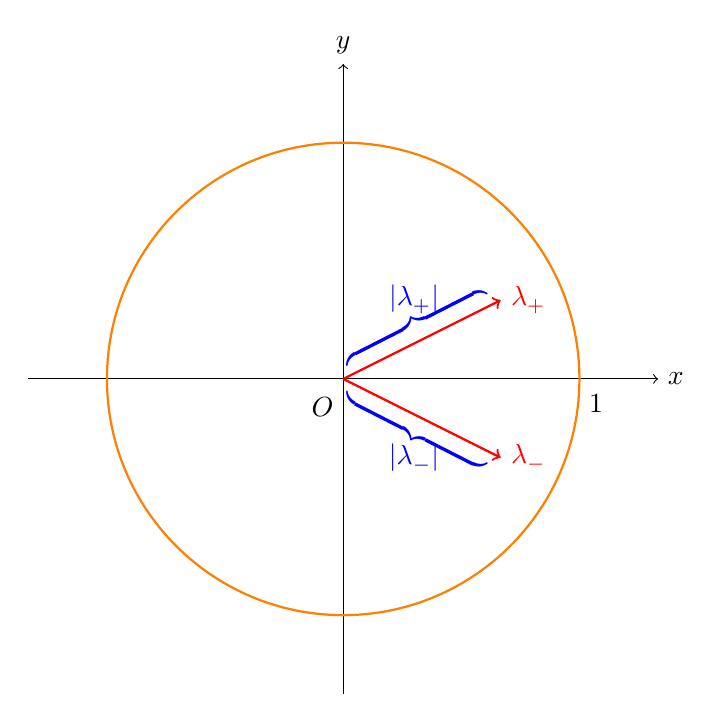
\begin{tikzpicture}
            \draw[->] (-4,0) -- (4,0)node[right]{$x$};
            \draw[->] (0,-4) -- (0,4)node[above]{$y$};
            \node[below=1em,left] at (0,0) {$O$};
            \draw (3,0.1) -- (3,-0.1)node[below=0.6em,right]{$1$};
            \draw[thick,orange] (0,0) circle (3);
            \draw[->,red,thick] (0,0) -- (2,1)node[right]{$\lambda_+$};
            \draw[->,red,thick] (0,0) -- (2,-1)node[right]{$\lambda_-$};
            \node[color=blue,rotate=207] at (0.9,0.7) {$\underbrace{\hspace{2cm}}$};
            \node[color=blue][above] at (0.9,0.7) {$|\lambda_+|$};
            \node[color=blue,rotate=333] at (0.9,-0.7) {$\underbrace{\hspace{2cm}}$};
            \node[color=blue,below] at (0.9,-0.7){$|\lambda_-|$};
        \end{tikzpicture}
    \end{center}
    \item $\lambda_\pm$是实数,此时有
    \begin{equation}
        4(t^2-t'^2)<\Delta^2
    \end{equation}
    由于无穷处狄利克雷条件,我们必须要求$|\lambda_\pm|<1$. 所以
    \begin{equation}
        \left|\lambda_{\pm}\right|^{2}=\frac{\Delta^{2}}{4\left(t+s t^{\prime}\right)^{2}}\left[2-\frac{4\left(t^{2}-t^{2}\right)}{\Delta^{2}} \pm 2 \sqrt{1-\frac{4\left(t^{2}-t^{2}\right)}{\Delta^{2}}}\right]<1
    \end{equation}
    这段计算冗长至极,求解$\Delta$
    \begin{equation}
        \begin{split}
            2-\frac{4(t^2-t'^2)}{\Delta^2}+2\sqrt{1-\frac{4(t^2-t'^2)}{\Delta^2}}&<\frac{4(t+st')^2}{\Delta^2}\\
            \Delta^2-2(t^2-t'^2)+\sqrt{\Delta^4-4\Delta^2(t^2-t'^2)}&<2(t+st')^2\\
            \Delta^4-4\Delta^2t^2+4\Delta^2t'^2<(4t^2+4stt'-\Delta^2)^2&=16t^4+16s^2t^2t'^2+\Delta^4+32st^3t'-8stt'\Delta^2-8t^2\Delta^2\\
            -\Delta^2t^2+\Delta^2t'^2&<4t^4+4t^2t'^2+8st^3t'-2stt'\Delta^2-2t^2\Delta^2\\
            \Longrightarrow(t^2+2stt'+t'^2)\Delta^2&<4(t^4+2st^3t'+t^2t'^2)(\text{左右两边除以$t^4$})\\
            (1+|\frac{t'}{t}|)^2\frac{\Delta^2}{t^2}<4(1+|\frac{t'}{t}|)^2&\Longrightarrow\Delta^2<4t^2
        \end{split}
    \end{equation}
    这样我们得到这种情况下$\Delta^2$必须满足条件:
    \begin{equation}
        4\left(t^{2}-t^{2}\right)<\Delta^{2}<4 t^{2}
    \end{equation}
\end{enumerate}
$j=0$时波函数要求是$\Psi_0=0$. 所以最终一维模型的解为
\begin{equation}
    \Psi_j=(\lambda_+^j-\lambda_-^j)\Psi,\quad\begin{pmatrix}
        (\lambda_+^1-\lambda_-^1)\Psi\\
        (\lambda_+^2-\lambda_-^2)\Psi\\
        \vdots\\
        (\lambda_+^N-\lambda_-^N)\Psi
    \end{pmatrix},\quad \Psi=\frac{1}{\sqrt{2}}\begin{pmatrix}
        1\\
        -is
    \end{pmatrix}
\end{equation}
这个解在$j=1$处并不是$0$.

一个特殊的例子:这个模型在$\Delta=0,t=t'$处存在两个精确解。这种情况下,我们有解
\begin{equation}
    \begin{aligned}
        \Psi_{L}=\left(\begin{array}{c}
        \varphi_{1} \\
        0 \\
        \vdots \\
        0
        \end{array}\right),\quad\Psi_{R}=\left(\begin{array}{c}
        0 \\
        0 \\
        \vdots \\
        \varphi_{N}
        \end{array}\right),\quad\lambda_{\pm}=\pm\sqrt{\frac{s-1}{s+1}}
        \end{aligned}
\end{equation}
在末端$j=1$处有条件$\varphi_N=\lambda^N\varphi_1\to0$,这就要求$s=1\Rightarrow\lambda=0$. 得到
\begin{equation}
    \Psi_{L}=\left(\begin{array}{c}
        \varphi_{1} \\
        0 \\
        \vdots \\
        0
        \end{array}\right),\quad\varphi_1=\frac{1}{\sqrt{2}}\begin{pmatrix}
            1\\
            -i
        \end{pmatrix}
\end{equation}
在末端$j=N$处有条件$\varphi_1=(\lambda^N)^{-1}\varphi_N\to0$,这就要求$s=-1\Rightarrow\lambda^{-1}=0$.得到
\begin{equation}
    \Psi_R=\begin{pmatrix}
        0\\
        0\\
        \vdots\\
        \varphi_N
    \end{pmatrix},\quad\varphi_N=\frac{1}{2}\begin{pmatrix}
        1\\
        i
    \end{pmatrix}
\end{equation}
这两个解分别局域在两个末端,能量本征值为$0$. 由于这两个解是简并的,它们的线性组合也是这个晶格模型的解。
\subsection{二维晶格模型}
\subsubsection{整数霍尔效应}
晶格模型中拓扑绝缘体的哈密顿为
\begin{equation}
    H=\frac{\hbar v}{a} \sum_{i=x, y, z} \sin k_{i} a \alpha_{i}+\left(m v^{2}-B \frac{4 \hbar^{2}}{a^{2}} \sum_{i=x, y, z} \sin ^{2} \frac{k_{i} a}{2}\right) \beta
\end{equation}
二维系统中$\alpha_x=\sigma_x,\alpha_y=\sigma_y,\beta=\sigma_z$. 这样我们可以把方晶格模型写成
\begin{equation}
    H=\mathbf{d}(\mathbf{k})\cdot\sigma
\end{equation}
其中
\begin{equation}
    \begin{split}
        &d_x=A\sin k_xa,\quad d_y=A\sin k_ya,\quad d_z=\Delta-4B(\sin^2\frac{k_xa}{2}+\sin^2\frac{k_ya}{2})\\
        &A=\frac{\hbar v}{a},\quad\Delta=mv^2,\quad\hbar=a=1
    \end{split}
\end{equation}
我们可以把这个哈密顿看成一个在有效磁场$\mathbf{d}(\mathbf{k})$里的自旋$\frac{1}{2}$系统。色散关系为
\begin{equation}
    E_{k,\pm}=\pm|\mathbf{d}(\mathbf{k})|
\end{equation}
色散关系的零点由下列决定
\begin{equation}
    \begin{split}
        &d_x^2=0\Longrightarrow\sin^2 k_xa=0,\quad d_y^2=0\Longrightarrow\sin^2k_ya=0\\
        &d_z^2=0\Longrightarrow\Delta-4B(\sin^2\frac{k_xa}{2}+\sin^2\frac{k_ya}{2})
    \end{split}
\end{equation}
存在三类解
\begin{enumerate}
    \item $\Delta=0,k_xa=0,k_ya=0$
    \item $\Delta=4B,k_xa=0,k_ya=\pi$或者$k_xa=\pi,k_ya=0$
    \item $\Delta=8B,k_xa=\pi,k_ya=\pi$
\end{enumerate}
能隙在这些点处关闭然后重新打开。我们将会看到在这些点处发生拓扑量子相变:$\Delta=0,4B,8B$

为了找到边缘态的解,我们可以采用带状的几何形状。沿着$x$方向,我们采用周期性边界条件使得$K_x$是一个好量子数。沿着$y$方向,我们采用一个开边界条件。对$x$方向做部分傅里叶变换,$k_x$被视为一个变量,问题简化为一个一维问题。
\begin{equation}
    \begin{split}
        H&=\sum_{k_x,k_y}c_{k_x,k_y}^\dagger h(k_x,k_y)c_{k_x,k_y}\\
        &\Downarrow\\
        H&=\sum_{k_x,k_y}\left[A\sin k_xac_{k_x,k_y}^\dagger\sigma_xc_{k_x,k_y}+A\sin k_yac_{k_x,k_y}^\dagger\sigma_yc_{k_x,k_y}+(\Delta-4B\sin^2\frac{k_xa}{2}-4B\sin^2\frac{k_ya}{2})c_{k_x,k_y}^\dagger\sigma_zc_{k_x,k_y}\right]\\
        &=\sum_{k_x,k_y}\left[A\sin k_xac_{k_x,k_y}^\dagger\sigma_xc_{k_x,k_y}+A\sin k_yac_{k_x,k_y}^\dagger\sigma_yc_{k_x,k_y}+(\Delta-4B\sin^2\frac{k_xa}{2}-2B+2B\cos k_ya)c_{k_x,k_y}^\dagger\sigma_zc_{k_x,k_y}\right]
    \end{split}
\end{equation}
对$k_y$做部分傅里叶变换
\begin{equation}
    \begin{cases}
        c_{k_x,j}&=\frac{1}{\sqrt{N_ya}}\sum_{k_y}e^{ik_yR_j}c_{k_x,k_y}\\
        c_{k_x,j}^\dagger&=\frac{1}{\sqrt{N_ya}}\sum_{k_y}e^{-ik_yR_j}c_{k_x,k_y}^\dagger
    \end{cases}\Longrightarrow\begin{cases}
        c_{k_x,k_y}=\frac{1}{\sqrt{N_ya}}\sum_{j}e^{-ik_yR_j}c_{k_x,j}\\
        c_{k_x,k_y}^\dagger=\frac{1}{\sqrt{N_ya}}\sum_{j}e^{ik_yR_j}c_{k_x,k_y}^\dagger
    \end{cases}
\end{equation}
同样的,分为四项来计算
\begin{equation}
    \begin{split}
        Term1&=\sum_{k_x,k_y}A\sin k_xac_{k_x,k_y}^\dagger\sigma_xc_{k_x,k_y}\\
        &\sum_{k_x,k_y}A\sin k_xa\frac{1}{N_ya}\sum_{j,j'}e^{ik_y(R_j-R_j')}c_{k_x,j}^\dagger\sigma_xc_{k_x,j'}\\
        &=\sum_{k_x}\sum_{j}A\sin k_xac_{k_x,j}^\dagger\sigma_xc_{k_x,j}
    \end{split}
\end{equation}
\begin{equation}
    \begin{split}
        Term2&=\sum_{k_x,k_y}A\sin k_yac_{k_x,k_y}^\dagger\sigma_yc_{k_x,k_y}\\
        &=\sum_{k_x,k_y}\frac{A}{2i}(e^{ik_ya}-e^{-ik_ya})\frac{1}{N_ya}\sum_{j,j'}e^{ik_y(R_j-R_{j'})}c_{k_x,j}^\dagger\sigma_yc_{k_x,j'}\\
        &=\sum_{k_x,k_y}-i\frac{A}{2}\frac{1}{N_ya}\sum_{j,j'}(e^{ik_y(R_j-R_{j'}+a)}-e^{ik_y(R_j-R_{j'}-a)})c_{k_x,j}^\dagger\sigma_yc_{k_x,j'}\\
        &=\sum_{k_x}\sum_{j}-i\frac{A}{2}(c_{k_x,j}^\dagger\sigma_yc_{k_x,j+1}-c_{k_x,j+1}^\dagger\sigma_yc_{k_x,j})
    \end{split}
\end{equation}
\begin{equation}
    \begin{split}
        Term3&=\sum_{k_x,k_y}(\Delta-4B\sin^2\frac{k_xa}{2}-2B)c_{k_x,k_y}^\dagger\sigma_zc_{k_x,k_y}\\
        &=\sum_{k_x,k_y}(\Delta-4B\sin^2\frac{k_xa}{2}-2B)\frac{1}{N_ya}\sum_{j,j'}e^{ik_y(R_j-R_{j'})}c_{k_x,j}^\dagger\sigma_zc_{k_x,j'}\\
        &=\sum_{k_x}\sum_{j}(\Delta-4B\sin^2\frac{k_xa}{2}-2B)c_{k_x,j}^\dagger\sigma_zc_{k_x,j}
    \end{split}
\end{equation}
\begin{equation}
    \begin{split}
        Term4&=\sum_{k_x,k_y}2B\cos k_ya\frac{1}{N_ya}\sum_{j,j'}e^{ik_y(R_j-R_{j'})}c_{k_x,j}^\dagger\sigma_zc_{k_x,j'}\\
        &=\sum_{k_x,k_y}\sum_{j,j'}\frac{B}{N_ya}(e^{ik_y(R_j-R_{j'}-a)}+e^{ik_y(R_j-R_{j'}-a)})c_{k_x,j}^\dagger\sigma_zc_{k_x,j'}\\
        &=\sum_{k_x}\sum_{j}B(c_{k_x,j}^\dagger\sigma_zc_{k_x,j+1}+c_{k_x,j+1}^\dagger\sigma_zc_{k_x,j})
    \end{split}
\end{equation}
四项合并得到
\begin{equation}
    H\left(k_{x}\right)=\sum_{j=1}^{N} c_{k_{k}, j}^{\dagger} h_{j, j}\left(k_{x}\right) c_{k_{x}, j}+\sum_{j=1}^{N-1}\left[c_{k_{x}, j}^{\dagger} h_{j, j+1}\left(k_{x}\right) c_{k_{x}, j+1}+c_{k_{x}, j+1}^{\dagger} h_{j+1, j}\left(k_{x}\right) c_{k_{x}, j}\right]
\end{equation}
其中
\begin{equation}
    \begin{aligned}
        h_{j, j}\left(k_{x}\right) &=A \sin k_{x} \sigma_{x}+\left(\Delta-2 B-4 B \sin ^{2} \frac{k_{x} a}{2}\right) \sigma_{z} \\
        h_{j, j+1}\left(k_{x}\right) &=B \sigma_{z}-\frac{i}{2} A \sigma_{y} \\
        h_{j+1, j}\left(k_{x}\right) &=h_{j, j+1}^{\dagger}\left(k_{x}\right)=B \sigma_{z}+\frac{i}{2} A \sigma_{y}
    \end{aligned}
\end{equation}
这个寻找边缘态解的问题简化成一个对于具体$k_x$的一维问题。我们可以通过之前介绍的方法求解这个问题,也可以通过数值来计算。
\subsubsection{量子自旋霍尔效应}
结合$2\times2$修正狄拉克模型可以生成一个量子自旋霍尔效应的有效模型。在时间反演$\Theta=i\sigma_yK$下
\begin{equation}
    k_i\longrightarrow-k_i,\quad\sigma_i\longrightarrow-\sigma_i
\end{equation}
我们有
\begin{equation}
    \begin{split}
        \Theta\mathbf{d}(\mathbf{k})\cdot\sigma\Theta^{-1}&=-\mathbf{d}(-\mathbf{k})\cdot\sigma\\
        &=A\sin k_xa\sigma_x+A\sin k_ya\sigma_y-(\Delta-4B\sin^2\frac{k_xa}{2}-4B\sin^2\frac{k_ya}{2})\sigma_z\\
        &=\begin{bmatrix}
            -d_z&d_x-id_y\\
            d_x+id_y&d_z
        \end{bmatrix}
    \end{split}
\end{equation}
也就是说在时间反演下的修正狄拉克模型实质上发生了
\begin{equation}
    d_x\longrightarrow d_x,\quad d_y\longrightarrow d_y,\quad d_z\longrightarrow-d_z
\end{equation}
我们令$\mathbf{d}(\mathbf{k})\cdot\sigma$为自旋向上部分,$-\mathbf{d}(-\mathbf{k})\cdot\sigma$为自旋向下部分。这种方式下,我们得到$4\times4$的有效哈密顿
\begin{equation}
    \begin{split}
        H_{QSHE}&=\begin{pmatrix}
            \mathbf{d}(\mathbf{k})\cdot\sigma&0\\
            0&-\mathbf{d}(-\mathbf{k})\cdot\sigma
        \end{pmatrix}=\begin{bmatrix}
            d_z&d_x-id_y&\quad&\quad\\
            d_x+id_y&-d_z&\quad&\quad\\
            \quad&\quad&-dz&d_x-id_y\\
            \quad&\quad&d_x+id_y&d_z
        \end{bmatrix}\\
        &=A\sin k_xas_0\otimes \sigma_x+A\sin k_yas_0\otimes\sigma_y+\left(\Delta-4B\sin^2\frac{k_xa}{2}-4B\sin^2\frac{k_ya}{2}\right)s_z\otimes\sigma_z
    \end{split}
\end{equation}
其中$s_0$是$2\times2$的单位矩阵,$s_z$是自旋指标的泡利矩阵。可以引入更多的项,例如出现在非对角项的自旋轨道耦合,耦合了自旋向上和自旋向下。这样$S_z$不再是守恒量。但是边缘态可能会保存下来,这可以用数值方法来验证。
\subsection{三维晶格模型}
三维方晶格模型为
\begin{equation}
    H=A \sum_{i=x, y, z} \alpha_{i} \sin k_{i} a+\beta\left(\Delta-4 B \sum_{i=x, y, z} \sin ^{2} \frac{k_{i} a}{2}\right)
\end{equation}
色散关系为
\begin{equation}
    \begin{split}
        E_{k,\pm}&=\pm|\mathbf{d}(\mathbf{k})|\\
        &=\pm \sqrt{A^{2} \sum_{i=x, y, z} \sin ^{2} k_{i} a+\left(\Delta-4 B \sum_{i=x, y, z} \sin ^{2} \frac{k_{i} a}{2}\right)^{2}}
    \end{split}
\end{equation}
能带零点由下列决定
\begin{equation}
    \begin{aligned}
        &\sin ^{2} k_{x} a=\sin ^{2} k_{y} a=\sin ^{2} k_{z} a=0\\
        &\Delta=4 B \sin ^{2} \frac{k_{x} a}{2}+4 B \sin ^{2} \frac{k_{y} a}{2}+4 B \sin ^{2} \frac{k_{z} a}{2}
        \end{aligned}
\end{equation}
有四个零点,分别是$\Delta=0,\Delta=4B,\Delta=8B$和$\Delta=12B$. 在$0<\Delta/B<4$和$8<\Delta<12$处是拓扑非平凡区。拓扑相变发生在$\Delta=0$和$\Delta=4,8,12$处。

为了找到表面态解,我们考虑一个半无穷大$x-y$平面。在这种情况下$k_x,k_y$仍然是好量子数。对$z$做部分傅里叶变换,变到$z$方向的局域格点上
\begin{equation}
    \begin{cases}
        c_{k_x,k_y,j_z}&=\frac{1}{\sqrt{N_za}}\sum_{k_z}e^{ik_zj_z}c_{k_x,k_y,k_z}\\
        c_{k_x,k_y,j_z}^\dagger&=\frac{1}{\sqrt{N_za}}\sum_{k_z}e^{-ik_zj_z}c_{k_x,k_y,k_z}^\dagger
    \end{cases},\quad\begin{cases}
        c_{k_x,k_y,k_z}&=\frac{1}{\sqrt{N_za}}\sum_{j_z}e^{-ik_zj_z}c_{k_x,k_y,j_z}\\
        c_{k_x,k_y,k_z}^\dagger&=\frac{1}{\sqrt{N_za}}\sum_{j_z}e^{ik_zj_z}c_{k_x,k_y,j_z}^\dagger
    \end{cases}
\end{equation}
得到一维$z$方向的有效哈密顿
\begin{equation}
    H(k_x,k_y)=\sum_{j_z}c_{k_{x}, k_{y}, j_{z}}^{\dagger} \epsilon\left(k_{x}, k_{y}\right) c_{k_{x}, k_{y}, j_{z}}+\sum_{j_z} c_{k_{x}, k_{y}, j_{z}+1}^{\dagger}\left(i \frac{A}{2} \alpha_{z}-2 B \beta\right) c_{k_{x}, k_{y}, j_{z}}+h . c .
\end{equation}
其中
\begin{equation}
    \epsilon\left(k_{x}, k_{y}\right)=\left(A \sin k_{x} \alpha_{x}+A \sin k_{y} \alpha_{y}\right)+\left(\Delta-2 B-4 B \sum_{i=x, y} \sin ^{2} \frac{k_{i} a}{2}\right) \beta
\end{equation}
这里$c_{k_x,k_y,j_z}$是四分量旋量。我们可以通过精确对角化找到表面态解。
\subsection{时间反演不变动量点的宇称TRIM}
通过把连续模型映射到格点模型,我们建立了一个晶格模型。在连续模型里,导带和价带的能隙在$k=0$处打开。在映射中,$k$被替换成$\frac{1}{a}\sin ka$. 因为$\sin ka$在$ka=0$和$ka=\pi$处有两个零点,所以这个性质可能让两个模型拓扑可分辨。系统的拓扑应该由布里渊区所有的能带结构决定,而不是仅仅由在单个点的渐进行为决定。在本节中,我们计算了本征态在时间反演不变动量下的宇称,这可以揭示格点模型在拓扑上是平凡的还是非平凡的。我们将会看到当两个能带之间的能隙关闭重新打开时,本征态的宇称发生改变,同时伴随着拓扑量子相变。

宇称算符$\pi$把右手系统变换到左手系统:
\begin{equation}
    \begin{split}
        \pi^\dagger x\pi&=-x\\
        \pi^\dagger p\pi&=-p
    \end{split}
\end{equation}
$\pi$不仅是幺正的还是厄米的:
\begin{equation}
    \pi^\dagger=\pi^{-1}=\pi
\end{equation}
此外还有$\pi^2=1$. 因此宇称算符的本征值要么是$1$要么是$-1$. 对于具有宇称的系统,如果是非简并的情况,能量本征态必定是对称的或者反对称的形式:
\begin{equation}
    [H,\pi]=0\Longrightarrow H\pi\phi(x)=\pi H\phi(x)=E\pi\phi(x)
\end{equation}
对于非简并态$\pi\phi(x)$和$\phi(x)$都属于同一个本征值$E$,所以必定是一个态,至少相差一个$U(1)$常数。记为
\begin{equation}
    \pi\phi(x)=C\phi(x)\Longrightarrow\pi^2\phi(x)=C^2\phi(x)=\phi(x)\Longrightarrow C^2=1\Longrightarrow C=\pm1
\end{equation}
所以对于非简并能级
\begin{equation}
    \pi\phi(x)=\phi(-x)=\pm\phi(x)
\end{equation}
需要在狄拉克方程里,全宇称算符$P$需要用$\beta$进行增广:
\begin{equation}
    P=\pi\beta
\end{equation}
这样:
\begin{equation}
    P\alpha_iP=-\alpha_i,\quad P\beta P=\beta
\end{equation}
这种方式下,狄拉克方程在宇称$P$下保持不变。
\subsubsection{一维晶格}
我们从一维晶格模型开始
\begin{equation}
    H=A\sin k_xa\alpha_x+\left(\Delta-4B\sin^2\frac{k_xa}{2}\right)\beta
\end{equation}
本征值是双重简并的:
\begin{equation}
    E_{\pm}=\pm\sqrt{A^2\sin^2k_xa+\left(\Delta-4B\sin^2\frac{k_xa}{2}\right)^2}
\end{equation}
假设费米能是$0$. 那么两个占据态有负能量值,并且相互之间时间反演。
\begin{equation}
    \psi_{1}=\left(\begin{array}{c}
        -\frac{A \sin k_{x} a}{\sqrt{2 E_{+}\left(E_{+}+\Delta-4 B \sin ^{2} \frac{k_{x} a}{2}\right)}} \\
        0 \\
        0 \\
        \frac{\Delta-4 B \sin ^{2} \frac{k_{x} a}{2}+E_{+}}{\sqrt{2 E_{+}\left(E_{+}+\Delta-4 B \sin ^{2} \frac{k_{x} a}{2}\right)}}
        \end{array}\right),\quad\Psi_2=\Theta\Psi_1
\end{equation}
系统在宇称$P$下不变
\begin{equation}
    PH(k)=H(-k)P
\end{equation}
注意$k$现在是一个好量子数,不是一个算符。由于这个关系,两个TRIM可以定义成
\begin{equation}
    PH(\Gamma_i)=H(\Gamma_i)P
\end{equation}
在一维情况下,满足上式的$\Gamma_i$一个是$\Gamma_1=0$:
\begin{equation}
    PH(\Gamma_1=0)=H(-\Gamma_1)P
\end{equation}
另一个是$\Gamma_2=\frac{\mathbf{K}}{2}=\frac{\pi}{a}$:
\begin{equation}
    PH(\Gamma_2)=H(-\Gamma_2+K)P
\end{equation}
计算$|\Psi_1\rangle$的宇称
\begin{equation}
    \delta|_{k=\Gamma_i}=\langle\psi_1|P|\psi_1\rangle=\mathrm{sgn}(-\Delta+4B\sin^2\frac{\Gamma_ia}{2})
\end{equation}
在这两个TRIM点,我们有
\begin{equation}
    \begin{split}
        \delta|_{ka=0}&=\mathrm{sgn}(-\Delta)\\
        \delta|_{ka=\pi}&=\mathrm{sgn}(-\Delta+4B)
    \end{split}
\end{equation}
我们注意到在$\Delta=0$和$\Delta=4B$处宇称符号发生改变,并且这里的能隙也是关闭的。我们定义$Z_2$指标
\begin{equation}
    (-1)^\nu=\delta|_{ka=0}\delta|_{ka=\pi}=\mathrm{sgn}(\Delta)\mathrm{sgn}(\Delta-4B)
\end{equation}
这样,存在两个明显的值$-1$和$1$. 对应的$\nu$为$0$或者$1$. 因此$0<\Delta^2<4\Delta B$范围内的$Z_2$指标为
\begin{equation}
    \nu=1
\end{equation}
这表示系统拓扑非平凡。
\subsubsection{二维模型}
对于二维晶格模型
\begin{equation}
    H=A \sum_{i=x, y} \sin k_{i} a \alpha_{i}+\left(\Delta-4 B \sum_{i=x, y} \sin ^{2} \frac{k_{i} a}{2}\right) \beta
\end{equation}
对应负能的两个能量本征态为
\begin{equation}
    \psi_1=\begin{pmatrix}
        \frac{-A\left(\sin k_{x} a-i \sin k_{y} a\right)}{\sqrt{2 E_{+}\left(E_{+}+\Delta-4 B\left(\sin ^{2} \frac{k_{x} a}{2}+\sin ^{2} \frac{k_{y} a}{2}\right)\right)}}\\
        0\\
        0\\
        \frac{\Delta-4 B\left(\sin ^{2} \frac{k_{x} a}{2}+\sin ^{2} \frac{k_{y} a}{2}\right)+E_{+}}{\sqrt{2 E_{+}\left(E_{+}+\Delta-4 B\left(\sin ^{2} \frac{k_{x} a}{2}+\sin ^{2} \frac{k_{y} a}{2}\right)\right)}}
    \end{pmatrix}
\end{equation}
同样的,两个本征态之间相互时间反演。$\psi_2=\Theta\psi_1$

对应的能量本征值为
\begin{equation}
    E_{-}=-\sqrt{A^{2} \sum_{i=x, y} \sin ^{2} k_{i} a+\left(\Delta-4 B \sum_{i=x, y} \sin ^{2} \frac{k_{i} a}{2}\right)^{2}}
\end{equation}
在TRIM点处的宇称同样的计算:
\begin{equation}
    \left.\delta\right|_{k=\Gamma_{i}}=\left\langle\psi_{1}|P| \psi_{1}\right\rangle=\operatorname{sgn}\left(-\Delta+4 B \sum_{i=x, y} \sin ^{2} \frac{\Gamma_{i} a}{2}\right)
\end{equation}
对于二维情况,有四个TRIM点$\Gamma_ia=(0,0),(0,\pi),(\pi,0),(\pi,\pi)$. 在这些点处,$\psi_1$的宇称为
\begin{equation}
    \begin{array}{l}
        \left.\delta\right|_{\Gamma_{i} a=(0,0)}=\operatorname{sgn}(-\Delta) \\
        \left.\delta\right|_{\Gamma_{i} a=(0, \pi)}=\operatorname{sgn}(-\Delta+4 B) \\
        \left.\delta\right|_{\Gamma_{i} a=(\pi, 0)}=\operatorname{sgn}(-\Delta+4 B) \\
        \left.\delta\right|_{\Gamma_{i} a=(\pi, \pi)}=\operatorname{sgn}(-\Delta+8 B)
        \end{array}
\end{equation}
同样的利用$Z_2$指标定义得到
\begin{equation}
    (-1)^{\nu}=\operatorname{sgn}(\Delta)[\operatorname{sgn}(-\Delta+4 B)]^{2} \operatorname{sgn}(\Delta-8 B)
\end{equation}
因此对于$0<\Delta^2<8\Delta B$范围内有非平凡指标
\begin{equation}
    \nu=1
\end{equation}
但是值得注意,在$\Delta=4B$处$\delta|_{ka=(0,\pi)}=\delta_{ka=(\pi,0)}$不连续。虽然在这个点附近$Z_2$指标等于$1$,但是存在拓扑量子相变。两个项都是拓扑非平凡的。随着相变发生,边界周围的自旋流将会改变符号。
\subsubsection{三维晶格}
类似一维二维的做法,具体不再赘述。
\section{拓扑不变量}
\subsection{布洛赫理论}
布洛赫波函数或者布洛赫态石电子在周期性势场里的波函数。我们考虑一个周期势场里的哈密顿$H(r)=H(r+R)$. 布洛赫定理告诉我们这样的系统本征态必定有这样的形式
\begin{equation}
    \left|\psi_{n, \mathbf{k}}(\mathbf{r})\right\rangle=e^{i \mathbf{k} \cdot \mathbf{r}}\left|u_{n, \mathbf{k}}(\mathbf{r})\right\rangle
\end{equation}
其中$u_{n,k}(r)$是晶格矢量$\mathbf{R}$的周期函数,$u_{n,k}(r)=u_{n,k}(r+R)$. $u_{n,k}(r)$是$H(k)=e^{-ik\cdot r}H(r)e^{ik\cdot r}$的本征态函数
\begin{equation}
    H(k)|u_{n,k}(r)\rangle=E_{n,k}|u_{n,k}(r)\rangle
\end{equation}
对应的能量本征之满足$E_{n}(k)=E_{n}(k+K)$,是倒格矢$K$的周期函数。能带指标$n$的能量关于$k$连续变化形成能带$n$. 对于给定$n$的能量本征值是关于$k$的周期函数。所有不同的$E_n(k)$值都位于倒格子的第一布里渊区。

根据泡利不相容原理,每一个态最多只能被一个电子占据。电子将首先充满较低的能态,从而形成电子密度有限的费米海。已占据态的最高能量被称为费米能级或费米能量。在费米能级附近,如果能带被部分占据,它就处于金属态。在这种情况下,当一个外场作用于系统,电场将迫使电子从平衡位置移动,并获得非零的总动量,形成电流。如果能带被完全填满,并且在满带(价带)与未填满的带(导带)之间存在能隙,则是绝缘态。在这种情况下,一个弱的外场不能迫使电子离开已占据态,使电流流通。这是绝缘体能带的图像。能隙的大小是半导体和绝缘体之间的分界线。如果能隙小于4ev(大约),尽管在绝对零度下,完全填充的电子带对电导率没有贡献,但在有限的温度下,电子可以很容易地从价带激发到导带。因此,半导体具有比绝缘体更小的能隙。
\subsection{Berry相位}
布洛赫波函数的选择并不是唯一确定,还存在一个相位不确定。例如
\begin{equation}
    |u_{n,k}\rangle\rightarrow e^{if(k)}|u_{n,k}\rangle
\end{equation}
仍然保持布洛赫定理的成立。布里渊区里确定一组相位叫做规范固定。对于时间反演不变系统,在布里渊区总是存在一个连续规范。对于非零Chern数时间反演破缺的系统,不存在这样的规范,连续规范不得不定义在布里渊区的不同片上。然而任何一个可观测物理量必须是规范无关的。

考虑一个与参数$R(t)$有关,随着时间缓慢变化的系统$R(0)\rightarrow R(t)$. 我们感兴趣的是系统从$t=0$到$t+T$的一个循环演化$R(0)=R(T)$. 参数$R(t)$在参数空间里沿着闭合路径$\mathcal{C}$缓慢变化。为了求解这个问题,我们首先引入一组$H(R(t))$本征态构成的瞬时基底
\begin{equation}
    H(R(t))|u_n(R(t))\rangle=E_n(R(t))|u_n(R(t))\rangle
\end{equation}
在绝热近似里,如果瞬时态相互之间分隔的很开并且时间演化非常缓慢,则系统一直保持在瞬时正交基底上。系统并不完全由这组基底$|u_n(R(t))\rangle$确定,因为还缺少相位的确定。但是我们可以要求函数沿着闭合路径是光滑单值的。这个方程也不能正确的描述量子态的含时演化。量子态随时间演化由含时薛定谔方程确定
\begin{equation}
    i\hbar\partial_t|\psi(t)\rangle=H(R(t))|\psi(t)\rangle
\end{equation}
由于$|u_n(R(t))\rangle$是一组完备的基底,$t$时刻波函数可以用这组完备基底线性展开
\begin{equation}
    |\psi(t)\rangle=\sum_{n}c_n|u_n(t)\rangle
\end{equation}
带入含时薛定谔方程得到
\begin{equation}
    i\hbar\sum_{n}\partial_tc_n(t)|u_n(t)\rangle+i\hbar\sum_{n}c_n(t)\partial_t|u_n(t)\rangle=\sum_{n}c_n(t)E_n(t)|u_n(t)\rangle
\end{equation}
用$\langle u_m(t)|$作用在上式得到
\begin{equation}\label{eq berry}
    i\hbar\partial_tc_m(t)+i\hbar\sum_{n}c_n(t)\langle u_m(t)|\partial_t|u_n(t)\rangle=c_m(t)E_m(t)
\end{equation}
为了计算第二项,我们考虑$H(t)|u_n(t)\rangle=E_n(t)|u_n(t)\rangle$两边同时对$t$求导,得到
\begin{equation}
    \partial_tH(t)|u_n(t)\rangle+H(t)\partial_t|u_n(t)\rangle=\partial_tE_n(t)|u_n(t)\rangle+E_n(t)\partial_t|u_n(t)\rangle
\end{equation}
用$\langle u_m(t)|$作用在上式得到
\begin{equation}
    \langle u_m(t)|\partial_tH(t)|u_n(t)\rangle-\partial_tE_n(t)\delta_{mn}=(E_n-E_m)\langle u_m(t)|\partial_t|u_n(t)\rangle
\end{equation}
对于$m\neq n$的情况
\begin{equation}
    \langle u_m(t)|\partial_t|u_n(t)\rangle=\frac{\langle u_m(t)|\partial_tH(t)|u_n(t)\rangle}{E_n(t)-E_m(t)}
\end{equation}
所以\eqref{eq berry}可以写成
\begin{equation}
    i\hbar\partial_tc_m(t)+i\hbar c_m(t)\langle u_m(t)|\partial_t|u_m(t)\rangle+i\hbar\sum_{n}c_n(t)\frac{\langle u_m(t)|\partial_tH(t)|u_n(t)\rangle}{E_n(t)-E_m(t)}=c_m(t)E_m(t)
\end{equation}
绝热近似认为$\langle u_m(t)|\partial_tH(t)|u_n(t)\rangle\ll E_n(t)-E_m(t)$,所以上式只能保留$m=n$项
\begin{equation}
    i\hbar\partial_t c_m(t)=c_m(t)E_m(t)-i\hbar c_m(t)\langle u_m(t)|\partial_t|u_m(t)\rangle
\end{equation}
这是$y'=a(x)y$型的常微分方程,通解为
\begin{equation}
    c_m(t)=c_m(t_0)e^{-\frac{i}{\hbar}\int_{t_0}^{t}\mathrm{d}t'E_m(t')}e^{-\int_{t_0}^{t}\mathrm{d}t'\langle u_m(t')|\frac{\partial}{\partial t'}|u_m(t')\rangle}
\end{equation}
波函数可以写成依赖于$|u_n(R(t))\rangle$的形式
\begin{equation}
    |\psi(t)\rangle=\sum_{n}e^{i\gamma_c^n}\exp\left[-\frac{i}{\hbar}\int_{0}^{t}dt'E_n(R(t'))\right]|u_n(R(t))\rangle
\end{equation}
几何相位$\gamma_c$随时间演化的关系
\begin{equation}
    \partial_t\gamma_c(t)=i\langle u_n(t)|\partial_t|u_n(t)\rangle
\end{equation}
在参数空间里,可以把几何相位写成参数空间里闭合路径的积分
\begin{equation}
    \gamma_c=\int_0^Tdt\;i\langle u_n(t)|\partial_t|u_n(t)\rangle=\int_C dR\cdot A^n(R)
\end{equation}
其中
\begin{equation}
    A^n(R)=i\langle u_n(R(t))|\nabla_R|u_n(R(t))\rangle
\end{equation}
这个向量叫做Berry联络或者Berry矢势。除了由$E_n(R(t'))$积分决定的动力学因子外,在绝热演化过程中量子态$|\psi(t)\rangle$还会获得一个额外的因子$\gamma_c$.

由于$A^n(R)$是规范相关的,所以当进行规范变换时
\begin{equation}
    \begin{split}
        &|u_n(R(t))\rangle\rightarrow e^{i\chi(R)}|u_n(R(t))\rangle\\
        &A^n(R)\rightarrow A^n(R)-\nabla_R\chi(R)
    \end{split}
\end{equation}
对于参数空间确定的一个初末点来说,相位$\gamma_c$将会改变$\chi(R(t=T))-\chi(R(t=T))$. 对于一个在闭合路径$\mathcal{C}$循环演化系统,有$R(0)=R(T)$. 波函数的单值性要求相位变化必须满足
\begin{equation}
    \chi(R(T))-\chi(R(0))=2m\pi
\end{equation}
这里$m$是整数。因此对于闭合路径$\mathcal{C}$,$\gamma_c$是与规范无关的值,叫做Berry相位
\begin{equation}
    \gamma_c=\oint_C dR\cdot A^n(R)
\end{equation}
利用Stokes定理,$\gamma_c$可以写成面积积分
\begin{equation}
    \gamma_c=\int_S dS\cdot\Omega^n(R)
\end{equation}
其中Berry曲率根据Berry联络来定义
\begin{equation}
    \Omega^n(R)=\nabla_R\times A^n(R)
\end{equation}
写成分量形式为
\begin{equation}
    \Omega_{\mu\nu}^n=\partial_\mu A_\nu^n-\partial_\nu A_\mu^n=i\left.\left(\left|\partial_{\mu} u_{n}(R)\right| \partial_{\nu} u_{n}(R)\right\rangle-\left\langle\partial_{\nu} u_{n}(R) | \partial_{\mu} u_{n}(R)\right\rangle\right)
\end{equation}
其中我们记$\frac{\partial}{\partial R_\mu}$为$\partial_\mu$. Berry曲率$\Omega$可以类比成电动力学里的磁场。由于瞬时基底满足关系式
\begin{equation}
    H|u_n(R(t))\rangle=E_n(R(t))|u_n(R(t))\rangle
\end{equation}
两边同时作用$\nabla_R$得到
\begin{equation}
    (\nabla_RH)|u_n\rangle+H\nabla_R|u_n\rangle=E_n\nabla_R|u_n\rangle
\end{equation}
两边乘以$\langle u_m|$得$(m\neq n)$
\begin{equation}
    \langle u_m|\nabla_R|u_n\rangle=\frac{\langle u_m|(\nabla_RH)|u_n\rangle}{E_n-E_m}
\end{equation}
对于$m=n$而言,由于归一化关系$\langle u_n|u_n\rangle=1$,两边作用微分算子$\nabla_R$得到
\begin{equation}
    \nabla_R\langle u_n|u_n\rangle=0\Rightarrow\langle u_n|\nabla_R|u_n\rangle+(\langle u_n|\nabla_R|u_n\rangle)^*=0
\end{equation}
这说明Berry联络中虽然有$i$,但$\langle u_n|\nabla_R|u_n\rangle$是纯虚数,所以Berry联络是一个实量。对于Berry曲率而言
\begin{equation}
    \begin{split}
        \Omega^n(R)&=\nabla_R\times A^n=\nabla_R\times i\langle u_n|\nabla_R|u_n\rangle\\
        &=i\langle\nabla_Ru_n|\times|\nabla_Ru_n\rangle+i\langle u_n|\nabla_R\times\nabla_R|u_n\rangle\\
        &=i\sum_m\langle\nabla_R u_n|u_m\rangle\times\langle u_m|\nabla u_n\rangle\\
        &=i\sum_m\langle u_m|\nabla_R|u_n\rangle^*\times\langle u_m|\nabla_R|u_n\rangle\\
        &=i\langle u_n|\nabla_R|u_n\rangle^*\times\langle u_n|\nabla_R|u_n\rangle+i\sum_{m\neq n}\frac{\langle u_n|(\nabla_RH)|u_m\rangle\times\langle u_m|(\nabla_RH)|u_n\rangle}{(E_n-E_m)^2}\\
        &=i\sum_{m\neq n}\frac{\langle u_n|(\nabla_RH)|u_m\rangle\times\langle u_m|(\nabla_RH)|u_n\rangle}{(E_n-E_m)^2}
    \end{split}
\end{equation}
写成指标形式:
\begin{equation}
    \Omega_\rho^n=\frac{i\epsilon_{\mu\nu\rho\langle u_n|\partial_\mu H|u_m\rangle\langle u_m|\partial_\nu H|u_n\rangle}}{(E_n-E_m)^2}
\end{equation}
上面利用了完备性关系$\sum_n|u_n(R)\rangle\langle u_n(R)|=1$. 我们考虑一个二能级系统,二能级系统的一般形式哈密顿可以写成形式
\begin{equation}
    H=\begin{bmatrix}
        Z&X-iY\\
        X+iY&-Z
    \end{bmatrix}=R\cdot\sigma
\end{equation}
能量本征值为$E_\pm=\pm|R|=\pm\sqrt{X^2+Y^2+Z^2}$,二能级在$|R|=0$处的简并点交叉。哈密顿的梯度为$\nabla_RH=\frac{1}{2}\sigma$,我们可以写出Berry曲率的矢量形式。为了简化起见,我们假设$R$沿着$z$方向
\begin{equation}
    \Omega_3^1=i\frac{\langle-|\frac{1}{2}\sigma_1|+\rangle\langle+|\frac{1}{2}\sigma_2|-\rangle-\langle-|\sigma_2|+\rangle\langle+|\frac{1}{2}\sigma_1|-\rangle}{(E_1-E_2)^2}=\frac{1}{2}\frac{1}{|R|^2}
\end{equation}
所以任意方向的Berry曲率为
\begin{equation}
    \Omega^1=\frac{1}{2}\frac{\mathbf{R}}{|R|^3}
\end{equation}
这个曲率可以被看成由在原点$\mathbf{R}=0$处的磁单极子生成的磁场。在包含磁单极子的球面上对Berry曲率积分,我们得到
\begin{equation}
    \frac{1}{2\pi}\int_S dS\cdot\Omega=1
\end{equation}
$\Omega$的散度满足
\begin{equation}
    \nabla_R\cdot\Omega=2\pi\delta(\mathbf{R})
\end{equation}
这样,点状的磁单极子位于$\mathbf{R}=0$并且产生Berry曲率。

在布洛赫能带里,Berry曲率定义为
\begin{equation}
    \Omega^n(k)=\nabla_k\times\langle u_n(k)|i\nabla_k|u_n(k)\rangle
\end{equation}
因为布里渊区中的两点$k,k+K$等价于相同的一点,其中$K$是倒格矢,所以闭合路径可以被认为$k$扫过全部的布里渊区。在这种情况下,Berry相位变成
\begin{equation}
    \gamma_c=\int_{BZ}dk\cdot\langle u_n(k)|i\nabla_k|u_n(k)\rangle
\end{equation}
\subsection{绝热输运计算量子霍尔电导和Chern数}
二维绝缘体带里的霍尔电导可以用Berry曲率来表示
\begin{equation}
    \sigma_{xy}=\frac{e^2}{\hbar}\int_{BZ}\frac{d^2k}{(2\pi)^2}\Omega_{k_x,k_y}=n\frac{e^2}{h}
\end{equation}
其中对于整数$n$是量子化的。考虑一个在弱外电场扰动下的晶格。通常静电势$\phi(r)$在空间中线性变化产生电场$E=-\nabla\phi$并且破坏了平移对称性。如果电场通过静电势进入哈密顿里,波矢量不再是一个好量子数,布洛赫定理对这种情况失效。为了避免这个困难,我们引入一个均匀的矢势$A(t)$,矢势随时间变化关系满足$\partial_tA=-E$. 这样哈密顿可以写成
\begin{equation}
    H(t)=\frac{1}{2m}(p+eA(t))^2+V(r)
\end{equation}
这里单位元电荷为$-e,e>0$. 这样通过这种方式,晶格的平移对称性得以保持,动向$p$仍然是一个好量子数。在动量空间里$p=\hbar q$. 我们有
\begin{equation}
    H(q,t)=H(q+\frac{e}{\hbar}A(t))
\end{equation}
我们引入一个规范不变的晶格动量
\begin{equation}
    k=q+\frac{e}{\hbar}A(t)
\end{equation}
由于$q$是一个好量子数,$\frac{\mathrm{d}q}{\mathrm{d}t}=0$,所以有
\begin{equation}
    \frac{\mathrm{d}k}{\mathrm{d}t}=-\frac{e}{\hbar}E
\end{equation}
速度算符定义为
\begin{equation}
    v=\frac{\mathrm{d}r}{\mathrm{d}t}=\frac{i}{\hbar}[H,r]
\end{equation}
在动量空间中,
\begin{equation}
    v(q)=\frac{1}{i\hbar}[r,H]=\frac{1}{i\hbar}i\hbar\frac{\partial H}{\partial p}=\frac{1}{\hbar}\nabla_q H,(p=\hbar q)
\end{equation}
$A(t)$的出现使得问题依赖于时间。量子态的波函数$\psi(t)$由含时薛定谔方程来决定
\begin{equation}
    i\hbar\partial_t|\psi(t)\rangle=H(t)|\psi(t)\rangle
\end{equation}
使用瞬时本征态基底组,我们可以将波函数$|\psi(t)\rangle$用瞬时基底$|u_n(t)\rangle$和本征值$E_n(t)$来展开。
\begin{equation}
    |\psi(t)\rangle=\sum_nc_n(t)e^{i\theta_n(t)}|u_n(t)\rangle,\quad \theta_n(t)=-\frac{1}{\hbar}\int_{t_0}^tE_n(t')\mathrm{d}t'
\end{equation}
上式带入含时薛定谔方程得到:
\begin{equation}
    i\hbar\sum_n\frac{\partial c_n(t)}{\partial t}e^{i\theta_n(t)}|u_n(t)\rangle+i\hbar\sum_nc_n(t)i\frac{\partial \theta_n(t)}{\partial t}e^{i\theta_n(t)}|u_n(t)\rangle+i\hbar\sum_nc_n(t)e^{i\theta_n(t)}\frac{\partial}{\partial t}|u_n(t)\rangle=\sum_nc_n(t)e^{i\theta_n(t)}E_n(t)|u_n(t)\rangle
\end{equation}
两边取$\langle u_m(t)|$得到
\begin{equation}
    \frac{\partial c_m(t)}{\partial t}=-\sum_nc_n(t)e^{i(\theta_n(t)-\theta_m(t))}\langle u_m(t)|\frac{\partial}{\partial t}|u_n(t)\rangle
\end{equation}
由于$H(t)|u_n(t)\rangle=E(t)|u_n(t)\rangle$,两边对$t$求导得到
\begin{equation}
    \frac{\partial H}{\partial t}|u_n(t)\rangle+H\frac{\partial}{\partial t}|u_n(t)\rangle=\frac{\partial E_n(t)}{\partial t}|u_n(t)\rangle+E_n(t)\frac{\partial}{\partial t}|u_n(t)\rangle
\end{equation}
上式两边取$\langle u_m(t)|,(m\neq n)$得到
\begin{equation}
    \langle u_m(t)|\frac{\partial H}{\partial t}|u_n(t)\rangle=\left[E_n(t)-E_m(t)\right]\langle u_m(t)|\frac{\partial}{\partial t}|u_n(t)\rangle
\end{equation}
上式带入$c_m(t)$满足的含时方程得到
\begin{equation}
    \frac{\partial c_m(t)}{\partial t}=-c_m(t)\langle u_m(t)|\frac{\partial}{\partial t}|u_m(t)\rangle-\sum_{n\neq m}c_n(t)e^{i(\theta_n(t)-\theta_m(t))}\frac{\langle u_m(t)|\frac{\partial H}{\partial t}|u_n(t)\rangle}{E_n(t)-E_m(t)}
\end{equation}
这表明,由于哈密顿依赖于时间,随着时间的推移,$n\neq m$的态将通过第二项与$|u_m(t)\rangle$发生混合。绝热近似的本质是认为哈密顿随着时间变化足够慢,远远慢于系统的自然频率,也就是说
\begin{equation}
    \frac{\langle u_m|\frac{\partial H}{\partial t}|u_n(t)\rangle}{E_n(t)-E_m(t)}=\frac{1}{\tau}\ll\langle u_m(t)|\frac{\partial}{\partial t}|u_m(t)\rangle
\end{equation}
这样在绝热近似下可以忽略第二项。容易计算出
\begin{equation}
    c_m(t)=e^{i\gamma_m(t)},\quad \gamma_m(t)=\int_{t_0}^{t}dt'i\langle u_m(t')|\frac{\partial}{\partial t'}|u_n(t')\rangle
\end{equation}
我们知道$c_m(t)$满足
\begin{equation}
    \frac{\partial c_m(t)}{\partial t}=-\sum_nc_n(t)e^{i(\theta_n(t)-\theta_m(t))}\langle u_m(t)|\frac{\partial}{\partial t}|u_n(t)\rangle
\end{equation}
我们考虑绝热过程,$R(t)$随着时间变化非常缓慢
\begin{equation}
    \langle u_n(q,t)|\partial_t u_n(q,t)\rangle=\partial_t R\cdot\langle u_n(q,R)|\nabla_R|u_n(q,R)\rangle\ll 1
\end{equation}
在极限$\partial_t R=0$的情况下,
\begin{equation}
    \partial_t c_n=0
\end{equation}
如果系统初始时在系统的本征态$|u_n(q,t)\rangle$,它将一直保持在这个本征态上不变。这就是量子绝热定理。

现在我们考虑$\partial_t R\neq0$,但$\partial_t R$很小的情况。假设初始态对于所有的$m\neq n$有$c_m(t_0)=0$,只有$c_n(t_0)=1$. 我们利用含时微扰理论来计算弱外电场下的量子修正。零阶微扰$c_m^{(0)}=\delta_{m,n}$,一阶微扰由下列给出
\begin{equation}
    \begin{split}
        \frac{\partial c_m^{(1)}(t)}{\partial t}&=-\sum_{n'}c_{n'}^{(0)}(t)\langle u_m(t)|\frac{\partial}{\partial t}|u_{n'}(t)\rangle e^{-\frac{i}{\hbar}\int_{t_0}^{t}(E_n(t')-E_m(t'))\mathrm{d}t'}\\
        &=-\langle u_m(t)|\frac{\partial}{\partial t}|u_n(t)\rangle e^{-\frac{i}{\hbar}\int_{t_0}^t(E_n(t')-E_m(t'))\mathrm{d}t'}
    \end{split}
\end{equation}
对于$m=n$的情况,$\frac{\mathrm{d}c_m^{(1)}(t)}{\mathrm{d}t}=0$. 这样我们有
\begin{equation}
    c_n^{(1)}(t)=0
\end{equation}
对于$m\neq n$,由于$e$指数因子随着时间的振动比较慢,我们可以看成常量,然后进行部分积分得到
\begin{equation}
    c_m^{(1)}(t)=-i\hbar\frac{\langle u_m(q,t)|\frac{\partial}{\partial t}|u_n(q,t)\rangle}{E_n-E_m}e^{-\frac{i}{\hbar}\int_{t_0}^t(E_n(t')-E_m(t'))\mathrm{d}t'}
\end{equation}
一阶微扰波函数为
\begin{equation}
    \begin{split}
        |\psi(t)\rangle&=|\psi^{(0)}\rangle+|\psi^{(1)}\rangle\\
        &=\sum_me^{-\frac{i}{\hbar}\int_{t_0}^t\mathrm{d}t'E_m(t')}\delta_{m,n}|u_m(q,t)\rangle+\sum_{m\neq n}e^{-\frac{i}{\hbar}\int_{t_0}^t\mathrm{d}t'E_m(t')}(-i\hbar)\frac{\langle u_m|\partial_t|u_n}{E_n-E_m}e^{-\frac{i}{\hbar}\int_{t_0}^t\mathrm{d}t'(E_n(t')-E_m(t'))}|u_m(q,t)\rangle\\
        &=e^{-\frac{i}{\hbar}\int_{t_0}^t\mathrm{d}t'E_n(t')}\left(|u_n(q,t)\rangle-i\hbar\sum_{m\neq n}\frac{\langle u_m(q,t)|\partial_t|u_n(q,t)\rangle}{E_n-E_m}|u_m(q,t)\rangle\right)
    \end{split}
\end{equation}
所以
\begin{equation}
    |u_n(t)\rangle=|u_n(q,t)\rangle-i\hbar\sum_{m\neq n}\frac{\langle u_m(q,t)|\partial_t|u_n(q,t)\rangle}{E_n-E_m}|u_m(q,t)\rangle
\end{equation}
在微扰水平上,计算速度算符$v(q)$的平均值,得到
\begin{equation}
    \begin{split}
        v_n(q)&=\frac{1}{\hbar}\langle u_n(t)|\nabla_q H|u_n(t)\rangle\\
        &=\frac{1}{\hbar}\langle u_n|\nabla_qH|u_n\rangle-i\sum_{m\neq n}\frac{\langle u_n|\nabla_qH|u_m\rangle\langle u_m|\partial_t|u_n\rangle}{E_n-E_m}+i\sum_{m\neq n}\frac{\langle\partial_t u_n|u_m\rangle\langle u_m|\nabla_qH|u_n\rangle}{E_n-E_m}\\
        &=\frac{1}{\hbar}\langle u_n|\nabla_qH|u_n\rangle-i\left(\frac{\langle u_n|\nabla_qH|u_m\rangle\langle u_m|\partial_t u_n\rangle}{E_n-E_m}-\frac{\langle\partial_t u_n|u_m\rangle\langle u_m|\nabla_qH|u_n\rangle}{E_n-E_m}\right)
    \end{split}
\end{equation}
对于第一项我们有
\begin{equation}
    \begin{split}
        Term1&=\frac{1}{\hbar}\langle u_n|\nabla_qH|u_n\rangle\\
        &=\frac{1}{\hbar}\langle u_n|\nabla_q(H|u_m\rangle)-\frac{1}{\hbar}\langle u_n|H\nabla_q|u_n\rangle\\
        &=\frac{1}{\hbar}\langle u_n|\nabla_qE_n|u_n\rangle+\frac{1}{\hbar}\langle u_n|E_n\nabla_q|u_n\rangle-\frac{1}{\hbar}\langle u_n|E_n\nabla_q|u_n\rangle\\
        &=\frac{1}{\hbar}\nabla_qE
    \end{split}
\end{equation}
对于第二项,我们先单独计算$\langle u_n|\nabla_qH|u_m\rangle$
\begin{equation}
    \begin{split}
        \langle u_n|\nabla_qH|u_m\rangle&=\nabla_q(\langle u_n|H)|u_m\rangle-\langle\nabla_qu_n|H|u_m\rangle\\
        &=E_n\langle\nabla_q u_n|u_m\rangle+\langle u_n|\nabla_qE|u_m\rangle-E_m\langle\nabla_qu_n|u_m\rangle\\
        &=(E_n-E_m)\langle\nabla_qu_n|u_m\rangle
    \end{split}
\end{equation}
将上式带入$v_n(q)$中得到
\begin{equation}
    \begin{split}
        v_n(q)&=\frac{1}{\hbar}\nabla_qE_n(q)-i\sum_{m\neq n}\left(\langle\nabla_qu_n|u_m\rangle\langle u_m|\partial_tu_n\rangle+\langle\partial_tu_n|u_m\rangle\langle\nabla_qu_m|u_n\rangle\right)\\
        &=\frac{1}{\hbar}\nabla_qE_n(q)-i\sum_{m\neq n}\left(\langle\nabla_qu_n|u_m\rangle\langle u_m|\partial_tu_n\rangle-\langle\partial_tu_n|u_m\rangle\langle u_m|\nabla_qu_n\rangle\right)\\
        &=\frac{1}{\hbar}\nabla_qE_n(q)-i\left(\langle\nabla_qu_n|\partial_tu_n\rangle-\langle\partial_tu_n|\nabla_qu_n\rangle\right)
    \end{split}
\end{equation}
定义
\begin{equation}
    \Omega_{q,t}^n=i\left(\langle\nabla_qu_n|\partial_tu_n\rangle-\langle\partial_tu_n|\nabla_qu_n\rangle\right)
\end{equation}
方程可以写成紧凑的形式
\begin{equation}
    v_n(q)=\frac{1}{\hbar}E_n(q)-\Omega_{q,t}^n
\end{equation}
这样在电场存在的情况下,电子可以获得一个反常横向速度,正比于能带的Berry曲率。

由于
\begin{equation}
    k=q+\frac{e}{\hbar}A(t),\quad\frac{\mathrm{d}k}{\mathrm{d}t}=-\frac{e}{\hbar}E
\end{equation}
我们有
\begin{equation}
    \nabla_q=\nabla_k,\partial_t=\partial_tk\cdot\nabla_k=-\frac{e}{\hbar}E\cdot\nabla_k
\end{equation}
很容易的到
\begin{equation}
    v_n(q)=\frac{1}{\hbar}\nabla_kE_n(k)-\frac{e}{\hbar}E\times\Omega^n(k)
\end{equation}
其中
\begin{equation}
    \begin{split}
        \Omega^n(k)&=\nabla_k\times\langle u_n(k)|i\nabla_k|u_n(k)\rangle\\
        &=i\langle\nabla_ku_n(k)|\times|\nabla_ku_n(k)\rangle
    \end{split}
\end{equation}
这样,外场在绝热过程中产生横向速度。电场产生的电流定义为
\begin{equation}
    j=-e\sum_n\int\frac{\mathrm{d}^2k}{(2\pi)^2}v_n(k)f(|k|)
\end{equation}
其中$f(|k|)$是费米狄拉克分布函数。假设费米面下所有的能带都填满了。第一项的求和由于对称性$E(k)=E(-k)$所以结果为$0$,第二项给出霍尔电流
\begin{equation}
    j=-e\sum_n\int_{BZ}\frac{\mathrm{d}^2k}{(2\pi)^2}(-\frac{e}{\hbar})E\times\Omega^n(k)
\end{equation}
求和$n$是对所有的满带求和
\begin{center}
    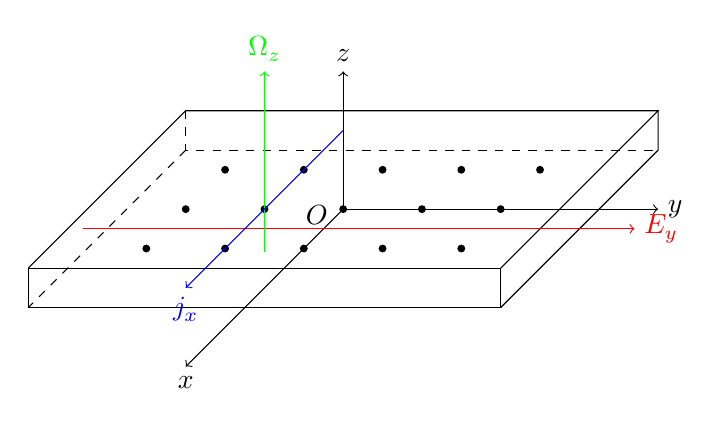
\begin{tikzpicture}
        \draw (0,0) rectangle (6,0.5);
        \draw (0,0.5) -- (2,2.5) -- (8,2.5) -- (6,0.5);
        \draw (6,0) -- (8,2) -- (8,2.5);
        \draw[dashed] (2,2.5) -- (2,2) -- (8,2);
        \draw[dashed] (2,2) -- (0,0);
        \fill[black] (1.5,0.75) circle (0.05);
        \fill[black] (2.5,0.75) circle (0.05);
        \fill[black] (3.5,0.75) circle (0.05);
        \fill[black] (4.5,0.75) circle (0.05);
        \fill[black] (5.5,0.75) circle (0.05);
        \fill[black] (2,1.25) circle (0.05);
        \fill[black] (3,1.25) circle (0.05);
        \fill[black] (4,1.25) circle (0.05);
        \fill[black] (5,1.25) circle (0.05);
        \fill[black] (6,1.25) circle (0.05);
        \fill[black] (2.5,1.75) circle (0.05);
        \fill[black] (3.5,1.75) circle (0.05);
        \fill[black] (4.5,1.75) circle (0.05);
        \fill[black] (5.5,1.75) circle (0.05);
        \fill[black] (6.5,1.75) circle (0.05);
        \draw[->] (4,1.25)node[below=0.2em,left=0.2em]{$O$} -- (8,1.25)node[right]{$y$};
        \draw[->] (4,1.25) -- (2,-0.75)node[below]{$x$};
        \draw[->] (4,1.25) -- (4,3)node[above]{$z$};
        \draw[->,red] (0.7,1) -- (7.7,1)node[right]{$E_y$};
        \draw[->,green] (3,0.7) -- (3,3)node[above]{$\Omega_z$};
        \draw[->,blue] (4,2.25) -- (2,0.25)node[below]{$j_x$};
    \end{tikzpicture}
\end{center}
取$\Omega^n(k)$为$z$方向
\begin{equation}
    j_\alpha=\frac{e^2}{2\pi h}\sum_n\int_{BZ}\mathrm{d}k_x\mathrm{d}k_y\Omega_{k_x,k_y}^n\epsilon_{\alpha\beta}E_\beta
\end{equation}
定义霍尔电导
\begin{equation}
    \sigma_H=\frac{e^2}{h}\frac{1}{2\pi}\sum_n\int_{BZ}\mathrm{d}k_x\mathrm{d}k_y\Omega_{k_x,k_y}^n
\end{equation}
所以霍尔电流可以写成
\begin{equation}
    j_\alpha=\sigma_H\epsilon_{\alpha\beta}E_\beta
\end{equation}
积分跑遍整个成第一布里渊区,并且有关系式
\begin{equation}
    \Omega_{k_x,k_y}^n=\Omega_{k_x+\pi,k_y}^n=\Omega_{k_x,k_y+\pi}^n
\end{equation}
因此第一布里渊区是一个闭合的Torus。在这个表达式里,我们假设了所有的能带都是满占据的,并且在价带和导带之间存在能隙。在闭合的Torus面上的积分给出一个整数$\nu$
\begin{equation}
    \sigma_H=\frac{e^2}{h}\sum_n\nu_n,\quad\sigma_H^n=\frac{e^2}{h}\nu_n
\end{equation}
这就是TKNN公式,$\nu_n$表示能带$n$的第一Chern数。我们现在具体计算一下上式,考虑一个二维晶格,晶格常数$a=1$. 根绝Berry曲率的定义,霍尔电导的表达式为
\begin{equation}
    \sigma_{xy}=\frac{e^2}{h}\frac{1}{2\pi}\int_0^{2\pi}\mathrm{d}k_x\int_0^{2\pi}\mathrm{d}k_y[\nabla_k\times A(k_x,k_y)]_z
\end{equation}
因此,Berry曲率确定的电导率简化为第一布里渊区的积分。

为了计算出这个曲面积分,可以利用Stokes公式。由于二维晶格第一布里渊区是单连通区域,我们可以把$T^2$上的曲面积分转化成一个周期条件下的方形区域积分,如图所示。通过这种方式,曲面积分可以简化为绕布里渊区的曲线积分。
\begin{center}
    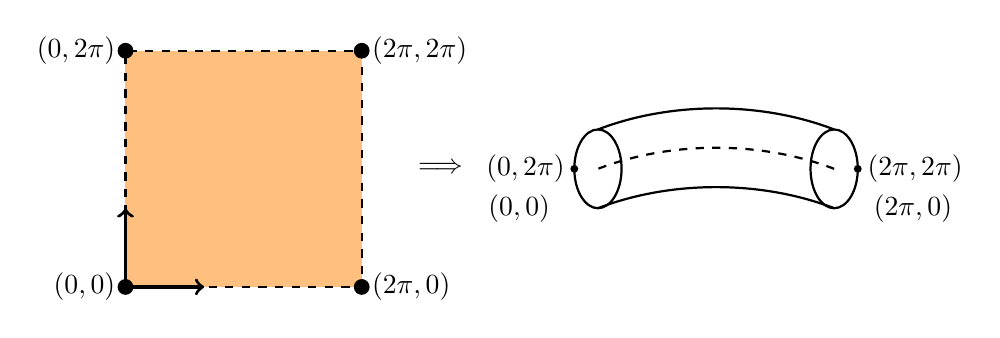
\begin{tikzpicture}
        \fill[orange,opacity=0.5] (0,0) rectangle (3,3);
        \draw[dashed,thick] (0,0) node[left]{$(0,0)$} -- (3,0) node[right]{$(2\pi,0)$} -- (3,3) node[right]{$(2\pi,2\pi)$} -- (0,3) node[left]{$(0,2\pi)$} -- cycle;
        \fill[black] (0,0) circle (0.1);
        \fill[black] (3,0) circle (0.1);
        \fill[black] (3,3) circle (0.1);
        \fill[black] (0,3) circle (0.1);
        \draw[->,very thick] (0,0) -- (1,0);
        \draw[->,very thick] (0,0) -- (0,1);
        \node at (4,1.5) {$\Longrightarrow$};
        \draw[thick] (9,1) arc (60:120:3 and 2);
        \draw[thick] (9,2) arc (60:120:3 and 2);
        \draw[dashed,thick] (9,1.5) arc (60:120:3 and 2);
        \draw[thick] (6,1.5) ellipse (0.3 and 0.5);
        \draw[thick] (9,1.5) ellipse (0.3 and 0.5);
        \fill[black] (5.7,1.5) node[left]{$(0,2\pi)$} circle (0.05);
        \node at (5,1) {$(0,0)$};
        \fill[black] (9.3,1.5) node[right]{$(2\pi,2\pi)$} circle (0.05);
        \node at (10,1) {$(2\pi,0)$};
    \end{tikzpicture}
\end{center}
\begin{equation}
    \begin{aligned}
        \sigma_{x y}^n=& \frac{e^{2}}{h} \frac{1}{2 \pi} \int_{0}^{2 \pi} d k_{x} \int_{0}^{2 \pi} d k_{y}\left[\partial_{k_{x}} \mathbf{A}_{y}^n\left(k_{x}, k_{y}\right)-\partial_{k_{y}} \mathbf{A}_{x}^n\left(k_{x}, k_{y}\right)\right] \\
        =& \frac{e^{2}}{h} \frac{1}{2 \pi} \int_{0}^{2 \pi} d k_{y}\left[\mathbf{A}_{y}^n\left(2 \pi, k_{y}\right)-\mathbf{A}_{y}^n\left(0, k_{y}\right)\right]-\frac{e^{2}}{h} \frac{1}{2 \pi} \int_{0}^{2 \pi} d k_{x}\left[\mathbf{A}_{x}^n\left(k_{x}, 2 \pi\right)-\mathbf{A}_{x}^n\left(k_{x}, 0\right)\right]
        \end{aligned}
\end{equation}
由于$|u_n(k_x,0)\rangle$和$|u_n(k_x,2\pi)\rangle$实际上表示一个相同的物理态,所以他们之间至多只能相差一个相因子
\begin{equation}
    \begin{split}
        |u_n(k_x,2\pi)\rangle&=e^{i\theta_x^n(k_x)}|u_n(k_x,0)\rangle\\
        |u_n(2\pi,k_y)\rangle&=e^{i\theta_y^n(k_y)}|u_n(0,k_y)\rangle
    \end{split}
\end{equation}
带入规范条件得到
\begin{equation}
    \begin{split}
        A_x^n(k_x,2\pi)&=A_x^n(k_x,0)-\partial_{k_x}\theta_x^n(k_x)\\
        A_y^n(2\pi,k_y)&=A_y^n(0,k_y)-\partial_{k_y}\theta_y^n(k_y)
    \end{split}
\end{equation}
我们假定相位函数是一个光滑函数,霍尔电导的积分化简为
\begin{equation}
    \begin{split}
        \sigma_{x,y}^n&=\frac{e^2}{h}\frac{1}{2\pi}\int_0^{2\pi}\mathrm{d}k_y[-\partial_{k_y}\theta_y^n(k_y)]-\frac{e^2}{h}\frac{1}{2\pi}\int_0^{2\pi}\mathrm{d}k_x[-\partial_{k_x}\theta_x(k_x)]\\
        &=\frac{e^2}{h}\frac{1}{2\pi}[\theta_y^n(0)-\theta_y^n(2\pi)+\theta_x^n(2\pi)-\theta_x^n(0)]
    \end{split}
\end{equation}
在布里渊区$T^2$的表面,四个波函数$|u(0,0)\rangle,|u(0,2\pi)\rangle,|u(2\pi,0)\rangle,|u(2\pi,2\pi)\rangle$实际上是一个物理态。使用这些态之间的相位关系
\begin{equation}
    \begin{split}
        |u_n(0,2\pi)\rangle&=e^{i\theta_x^n(0)}|u_n(0,0)\rangle\\
        |u_n(2\pi,2\pi)\rangle&=e^{i\theta_x^n(2\pi)}|u_n(2\pi,0)\rangle\\
        |u_n(2\pi,0)\rangle&=e^{i\theta_y^n(0)}|u_n(0,0)\\
        |u_n(2\pi,2\pi)\rangle&=e^{i\theta_y^n(2\pi)}|u_n(0,2\pi)\rangle
    \end{split}
\end{equation}
所以得到
\begin{equation}
    \begin{split}
        |u_n(0,0)\rangle&=e^{-i\theta_x^n(0)}|u_n(0,2\pi)\rangle\\
        &=e^{-i(\theta_y^n(2\pi)+\theta_x^n(0))}|u_n(2\pi,2\pi)\rangle\\
        &=e^{i(\theta_x^n(2\pi)-\theta_y^n(2\pi)-\theta_x^n(0))}|u_n(2\pi,0)\rangle\\
        &=e^{i(\theta_y^n(0)+\theta_x^n(2\pi)-\theta_y^n(2\pi)-\theta_x^n(0))}|u_n(0,0)\rangle
    \end{split}
\end{equation}
由于波函数的单值性,必须有
\begin{equation}
    \theta_{x}^n(0)+\theta_{y}^n(2 \pi)-\theta_{x}^n(2 \pi)-\theta_{y}^n(0)=2 \nu_n \pi
\end{equation}
所以霍尔电导满足TKNN关系
\begin{equation}
    \sigma_{x,y}^n=\frac{e^2}{h}\nu_n,\quad\sigma_{x,y}=\frac{e^2}{h}\sum_n\nu_n
\end{equation}
因此当能带是满带时,霍尔电导必定是整数量子化的。整数$\nu_n$叫做TKNN数或者叫第一Chern数,这表征了布洛赫态$|u_n(k_x,k_y)\rangle$在参数空间$\{k_x,k_y\}$的拓扑结构。
\subsection{拓扑平带计算霍尔电导和Chern数}
\subsubsection{流算符}
为了找到在外场下的哈密顿线性响应形式,我们先考虑一个一般的单体无相互作用哈密顿:
\begin{equation}
    H=\sum_{i,j,\alpha,\beta}(c_{i,\alpha}^\dagger t_{ij}^{\alpha\beta}c_{j,\beta}-\mu c_{i,\alpha}^\dagger c_{j,\beta})
\end{equation}
$i,j$是格点指标,$\alpha,\beta$是轨道指标(例如自旋,轨道,或者其他量子数)。$h_{ij}^{\alpha\beta}$是$\alpha$轨道到$\beta$轨道的$i,j$之间的隧穿振幅。假设一共有$m$个轨道。因为我们可以把原胞内的不同位点看成额外的指标,所以如果单位原胞里有两个位点,例如石墨烯,可以写成这种形式。我们假设系统具有平移不变性,这意味着$h_{ij}^{\alpha\beta}=h_{i-j}^{\alpha\beta}$. 我们做一个傅里叶变换。
\begin{equation}
    c_{j,\alpha}=\frac{1}{V}\sum_k e^{ik\cdot R_j}c_{k,\alpha}
\end{equation}
简单计算一下
\begin{equation}
    \begin{split}
        H&=\sum_{i,j,\alpha,\beta}\frac{1}{V}\left(\sum_{k,k'}e^{-ik\cdot R_i}e^{ik'\cdot R_j}c_{k,\alpha}^\dagger h_{ij}^{\alpha\beta}c_{k',\beta}-\sum_{k,k'}\mu c_{k,\alpha}^\dagger c_{k',\beta}\delta_{ij}\delta_{\alpha\beta}e^{-ik\cdot R_i}e^{ik\cdot R_j}\right)\\
        &=\frac{1}{V}\sum_{i,j,\alpha,\beta}\sum_{k,k'}e^{-ik\cdot(R_i-R_j))}e^{i(k'-k)\cdot R_j}c_{k,\alpha}^\dagger h_{ij}^{\alpha\beta}c_{k',\beta}-\frac{1}{V}\sum_{j,\alpha,k,k'}\mu c_{k,\alpha}^\dagger c_{k',\alpha}e^{-i(k'-k)\cdot R_j}\\
        &=\frac{1}{V}\sum_{j,i-j,\alpha,\beta}\sum_{k,k'}e^{-ik\cdot (R_i-R_j)}e^{i(k'-k)\cdot R_j}c_{k,\alpha}^\dagger h_{ij}^{\alpha\beta}c_{k',\beta}-\frac{1}{V}\sum_{j,\alpha,k,k'}\mu c_{k,\alpha}^\dagger c_{k',\alpha}e^{-i(k'-k)\cdot R_j}\\
        &=\sum_{k,\alpha,\beta,i-j}e^{-ik\cdot (R_i-R_j)}c_{k,\alpha}^\dagger h_{ij}^{\alpha\beta}c_{k,\beta}-\sum_{k,\alpha}\mu c_{k,\alpha}^\dagger c_{k,\alpha}
    \end{split}
\end{equation}
定义
\begin{equation}
    \begin{split}
        \epsilon_{\alpha\beta}(k)&=\sum_{i-j}t_{ij}^{\alpha\beta}e^{-ik\cdot (R_i-R_j)}-\mu\delta_{\alpha\beta}\\
        &\Downarrow\\
        H&=\sum_{k,\alpha,\beta}c_{k,\alpha}^\dagger\epsilon_{\alpha\beta}(k)c_{k,\beta}
    \end{split}
\end{equation}
$N$是晶格位点的总数。这里$k$是波矢,依赖于空间的维数。哈密顿的傅里叶变换表明了化学势包含在矩阵$\epsilon$里。得到流算符的表达式有两种不同的办法,其中一个用于线性响应计算,另一个用于晶格磁场中电子的Hofstadter问题
\subsubsection{连续方程得到流算符}
电流的连续性方程为
\begin{equation}
    \frac{\partial\rho}{\partial t}+\nabla\cdot J(x)=0
\end{equation}
傅里叶变换后得到$q$空间表达式
\begin{equation}
    \frac{\partial\rho}{\partial t}-iq\cdot J(q)=0
\end{equation}
其中算符在晶格中的傅里叶变换为
\begin{equation}
    A_j=\frac{1}{\sqrt{V}}\sum_{k}A_ke^{ik\cdot R_j}
\end{equation}
格点坐标的密度算符表示为$\rho_i=c_i^\dagger c_i$,它的傅里叶变换为
\begin{equation}
    \rho(q)=\frac{1}{\sqrt{V}}\sum_i\rho_ie^{iq\cdot R_i}=\frac{1}{\sqrt{V}}\sum_{k}c_{k+q}^\dagger c_k
\end{equation}
所以连续性方程可以写成
\begin{equation}
    -iq\cdot J(q)=-\frac{\partial\rho_q}{\partial t}=i[\rho(q),H]=i[\frac{1}{\sqrt{V}}\sum_{k}c_{k+q}^\dagger c_k,\sum_p \epsilon_p c_p^\dagger c_p]
\end{equation}
展开计算一下得到
\begin{equation}
    q\cdot J(q)=\frac{1}{\sqrt{V}}\sum_{k}(\epsilon_{k+q}-\epsilon_k)c_{k+q}^\dagger c_k
\end{equation}
考虑长波极限,$q\to 0$,我们感兴趣的是低能极限。如果场的变化比晶格空间还要大,那么这个低能近似是一个良好的近似。我们可以做一个近似替换
\begin{equation}
    \epsilon_{k+q}-\epsilon_k\approx\frac{\partial\epsilon_k}{\partial k}\cdot q
\end{equation}
但这个仅仅只对$q$的一阶有效。为了能展开到二阶,我们做一个替换$k\rightarrow k-\frac{q}{2}$
\begin{equation}
    \begin{split}
        q\cdot J(q)&=\frac{1}{\sqrt{V}}\sum_k(\epsilon_{k+\frac{q}{2}}-\epsilon_{k-\frac{q}{2}})c_{k+\frac{q}{2}}^\dagger c_{k-\frac{q}{2}}\\
        &=\frac{1}{\sqrt{V}}\sum_k(\frac{\partial\epsilon_k}{\partial k}\cdot q)c_{k+\frac{1}{2}}^\dagger c_{k-\frac{q}{2}}+\mathcal{O}(q^2)
    \end{split}
\end{equation}
线性项$q$在一些情况下非常重要,因此这个平移非常关键。至此,我们得到了流算符表达形式:
\begin{equation}
    J(q)=\frac{1}{\sqrt{V}}\sum_{k}c_{k+\frac{q}{2}}^\dagger\frac{\partial\epsilon_k}{\partial k}c_{k-\frac{q}{2}}
\end{equation}
\subsubsection{Peierls替换得到流算符}
麦克斯韦方程组为
\begin{equation}
    \begin{cases}
        \nabla\cdot E=\frac{\rho}{\epsilon_0}\\
        \nabla\times E=-\frac{\partial B}{\partial t}\\
        \nabla\cdot B=0\\
        \nabla\times E=\mu_0J+\mu_0\epsilon_0\frac{\partial E}{\partial t}
    \end{cases}\Longrightarrow\begin{cases}
        E=-\nabla\phi-\frac{\partial A}{\partial t}\\
        B=\nabla\times A
    \end{cases}
\end{equation}
电磁场洛伦兹力的表达式为
\begin{equation}
    F=q(E+v\times B)
\end{equation}
所以我们得到
\begin{equation}
    \begin{split}
        F&=q\left[-\nabla\phi+v\times(\nabla\times A)-\frac{\partial A}{\partial t}\right]\\
        &=q\left[-\nabla\phi+\nabla(v\cdot A)-(v\cdot\nabla)A-\frac{\partial A}{\partial t}\right]
    \end{split}
\end{equation}
在拉格朗日力学里,广义力的表达式为
\begin{equation}
    F_i=-\frac{\partial U}{\partial q_i}+\frac{\mathrm{d}}{\mathrm{d}t}\left(\frac{\partial U}{\partial\dot{q}_i}\right),\quad\mathbf{F}=-\nabla U+\frac{\mathrm{d}}{\mathrm{d}t}\nabla_v U
\end{equation}
观察上式表达式可知$(v\cdot\nabla)A+\frac{\partial A}{\partial t}=\frac{\mathrm{d}}{\mathrm{d}t}A$. 可以知道
\begin{equation}
    \nabla_vU=-qA,\quad-\nabla U=-\nabla(q\phi-qv\cdot A)
\end{equation}
所以可以得到电磁场广义势的最小耦合形式
\begin{equation}
    U=-qv\cdot A+q\phi
\end{equation}
得到带电粒子在电磁场中的拉氏量为
\begin{equation}
    L=T-U=\frac{1}{2}m\dot{x}^2+q\dot{x}\cdot A-q\phi
\end{equation}
写成分量形式为:
\begin{equation}
    L=\sum_{i}\frac{1}{2}m\dot{x}_i^2+\sum_iq\dot{x}_iA_i-q\phi
\end{equation}
正则动量为
\begin{equation}
    p_i=\frac{\partial L}{\partial\dot{x}_i}=m\dot{x}_i+qA_i
\end{equation}
定义机械动量$\Pi_i=m\dot{x}_i$得到机械动量和正则动量之间的关系
\begin{equation}
    \Pi_i=p_i-qA
\end{equation}
对拉氏量做勒让德变换得到
\begin{equation}
    H=\sum_{i}\dot{x}_ip_i-L=\sum_i\frac{1}{2}m\dot{x}_i^2+q\phi
\end{equation}
带入机械动量得到
\begin{equation}
    H=\sum_i\frac{(p_i-qA_i)^2}{2m}+q\phi
\end{equation}
所以对于有磁场的哈密顿,有最小耦合形式$p\rightarrow p-qA$. 由于麦克斯韦方程组,可以得到规范变换
\begin{equation}
    \begin{cases}
        A\rightarrow A+\nabla\Lambda\\
        \phi\rightarrow\phi+\frac{\partial\Lambda}{\partial t}
    \end{cases}
\end{equation}
规范变换不影响可观测物理量,例如我们所观测的机械动量$\Pi=p-qA$. 这样�������们有
\begin{equation}
    \begin{split}
        &A\longrightarrow\tilde{A}=A+\nabla\Lambda\\
        &|\psi\rangle\longrightarrow|\tilde{\psi}\rangle=U|\psi\rangle\\
        &\langle\psi|p-qA|\psi\rangle=\langle\tilde{\psi}|p-q\tilde{A}|\tilde{\psi}\rangle\Longrightarrow U^\dagger(p-qA-q\nabla\Lambda)U=p-qA
    \end{split}
\end{equation}
这样我们得到$U=\exp(iq\Lambda)$,也就是说对于波函数而言,规范变换是指$U(1)$变换
\begin{equation}
    |\psi\rangle\Longrightarrow e^{iq\Lambda}|\psi\rangle
\end{equation}
下对于可观测量保持不变。我们现在考虑一个格点系统
\begin{center}
    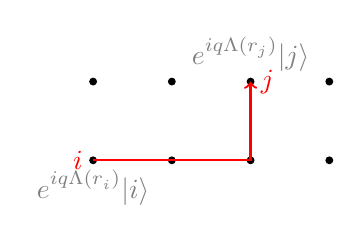
\begin{tikzpicture}
        \fill[black] (0,0) circle (0.05);
        \fill[black] (1,0) circle (0.05);
        \fill[black] (2,0) circle (0.05);
        \fill[black] (3,0) circle (0.05);
        \fill[black] (0,1) circle (0.05);
        \fill[black] (1,1) circle (0.05);
        \fill[black] (2,1) circle (0.05);
        \fill[black] (3,1) circle (0.05);
        \draw[thick,red,->] (0,0)node[left]{$i$} -- (2,0) -- (2,1)node[right]{$j$};
        \node[below,gray] at (0,0) {$e^{iq\Lambda(r_i)}|i\rangle$};
        \node[above,gray] at (2,1) {$e^{iq\Lambda(r_j)}|j\rangle$};
    \end{tikzpicture}
\end{center}
$i$格点上的产生算符定义为
\begin{equation}
    |i\rangle=c_i^\dagger|0\rangle
\end{equation}
我们考虑晶格系统具有一个局域的规范变换$\Lambda(r_i)$,格点$i,j$处的规范变换分别为
\begin{equation}
    c_i^\dagger\longrightarrow c_i^\dagger e^{iq\Lambda(r_i)},\quad A\longrightarrow A+\nabla\Lambda
\end{equation}
如果系统没有磁场,我们可以通过选择合适的规范$\Lambda$来消除$A$使得它为$0$. 紧束缚模型Hopping项在这个规范下可以写成
\begin{equation}
    H=t_{ij}e^{iq(\Lambda(r_i)-\Lambda(r_j))}c_i^\dagger c_j=t_{ij}e^{iq\int_{r_j}^{r_i}drA(r)}c_i^\dagger c_j
\end{equation}
这个表达式是由零磁场导出的,通过选择积分路径作为最近邻键之间的最短距离,这个表达式被用于在晶格模型中包含磁场。这被称为晶格中的Peierls替换。

现在我们回到晶格系统,我们可以直接从在外场的矢势作用下的紧束缚近似哈密顿直接得到流算符。无电磁场哈密顿中的隧穿振幅$t_{ij}^{\alpha\beta}$来自于不同格点的不同轨道之间的交叠积分。对于有磁场的哈密顿,在做紧束缚近似之前我们需要做一个替换$p\rightarrow p-eA$. 

在格点系统里,最小耦合形式是Peierls替换$t_{ij}\rightarrow t_{ij}e^{ie\int_{r_j}^{r_i}drA(r)},(e<0)$,其中$A$是依赖于空间分布的电磁矢势。当我们绕着一个被单位磁通穿过的小板时,这个替换会产生一个等于$2\pi$的相位
\begin{center}
    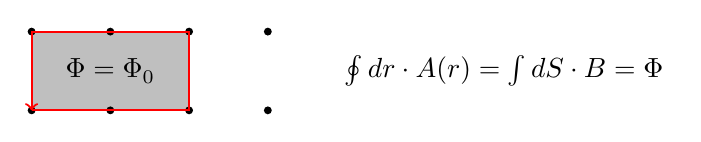
\begin{tikzpicture}
        \fill[gray,opacity=0.5] (0,0) rectangle (2,1);
        \fill[black] (0,0) circle (0.05);
        \fill[black] (1,0) circle (0.05);
        \fill[black] (2,0) circle (0.05);
        \fill[black] (3,0) circle (0.05);
        \fill[black] (0,1) circle (0.05);
        \fill[black] (1,1) circle (0.05);
        \fill[black] (2,1) circle (0.05);
        \fill[black] (3,1) circle (0.05);
        \draw[->,red,thick] (0,0) -- (2,0) -- (2,1) -- (0,1) -- (0,0);
        \node at (1,0.5) {$\Phi=\Phi_0$};
        \node at (6,0.5) {$\oint dr\cdot A(r)=\int dS\cdot B=\Phi$};
    \end{tikzpicture}
\end{center}
由于单位磁通可以通过规范变换消除,皮尔斯替换对实际可观测物理量没有影响。:现在有一个明显的不确定性:在两个格点$i$和$j$之间获得的相位取决于它们之间的路径。我们通过选择连接两点的最短直线路径来解决这个不确定性。如果矢势在积分路径上变化不大,我们可以使用线性近似:
\begin{equation}
    \int_{R}^{R'}A(s,t)\cdot ds\approx(R'-R)\cdot\frac{1}{2}(A(R',t)-A(R,t))\approx(R'-R)\cdot\frac{1}{2}A(\frac{R'+R}{2},t)
\end{equation}
因为我们想要处理线性响应,我们将哈密顿展开到矢势$A$的一阶项。为了得到通常地反磁项,我们需要把哈密顿展开到二阶。然而,我们在这里不分析这个项,因为它在空间指标中是对角的,我们只对非对角(霍尔)响应感兴趣。泰勒展开为
\begin{equation}
    H=\sum_{i,j,\alpha,\beta}c_{i,\alpha}^\dagger t_{ij}^{\alpha,\beta}e^{ie\int_{r_i}^{r_j}drA(r)}c_{j,\beta}\approx\sum_{i,j,\alpha,\beta}c_{i,\alpha}^\dagger t_{ij}^{\alpha\beta}(1+ie\int_{r_i}^{r_j}dr\cdot A(r))c_{j,\beta}=H_0+H_{ext}
\end{equation}
其中$H_{ext}$是哈密顿由于外场的改变。我们令$\rho=r_i-r_j$,注意到系统在无外电磁场条件下满足平移不变性,所以隧穿振幅$t_{ij}=t_{i-j}=t_\rho$
\begin{equation}
    \begin{split}
        H_{ext}&=\sum_{k_1,k_2,\alpha,\beta}c_{k_1,\alpha}^\dagger c_{k_2,\beta}\frac{1}{V}\sum_{i,j}e^{ik_2\cdot r_j}e^{-ik_1\cdot r_i}t_{ij}^{\alpha\beta}ie\int_{r_j}^{r_i}A(l)\cdot dl\\
        &=\sum_{k_1,k_2,\alpha,\beta}c_{k_1,\alpha}^\dagger c_{k_2,\beta}\frac{1}{V}\sum_{j,\rho}e^{i(k_2-k_1)r_j}e^{-ik_1\rho}t_{ij}^{\alpha\beta}ie\int_{r_j}^{r_i}A(l)\cdot dl\\
        &\approx\sum_{k_1,k_2,\alpha,\beta}c_{k_1,\alpha}^\dagger c_{k_2,\beta}\frac{1}{V}\sum_{j,\rho}e^{i(k_2-k_1)r_j}e^{-ik_1\rho}t_{ij}^{\alpha\beta}ie\rho\cdot A(r_j+\frac{\rho}{2})\\
    \end{split}
\end{equation}
带入$A$的傅里叶变换
\begin{equation}
    A(r_j)=\frac{1}{\sqrt{V}}\sum_{q}e^{-iq\cdot r_j}A(q)
\end{equation}
得到
\begin{equation}
    \begin{split}
        H_{ext}&=\sum_{k_1,k_2,\alpha,\beta}c_{k_1,\alpha}^\dagger c_{k_2,\beta}\frac{1}{V^{\frac{3}{2}}}\sum_{j,\rho,q}e^{i(k_2-k_1-q)r_j}e^{-i(k_1+\frac{q}{2})\rho}t_{ij}^{\alpha\beta}ie\rho\cdot A(q)\\
        &=\sum_{k_1,k_2,\alpha,\beta}c_{k_1,\alpha}^\dagger c_{k_2,\beta}\frac{1}{\sqrt{V}}\sum_{\rho,q}\delta_{k_2,k_1+q}e^{-i(k_1+\frac{q}{2})\rho}t_{ij}^{\alpha\beta}ie\rho\cdot A(q)\\
        &=\frac{1}{\sqrt{V}}\sum_{k_1,\alpha,\beta,\rho,q}c_{k_1,\alpha}^\dagger c_{k_1+q,\beta}e^{-i(k_1+\frac{q}{2})\rho}t_{ij}^{\alpha\beta}ie\rho\cdot A(q)
    \end{split}
\end{equation}
做一个平移$k_1+\frac{q}{2}=k$
\begin{equation}
    \begin{split}
        H_{ext}&=\frac{1}{\sqrt{V}}\sum_{k,q,\alpha,\beta,\rho}c_{k-\frac{q}{2},\alpha}^\dagger c_{k+\frac{q}{2},\beta}t_{ij}^{\alpha\beta}ie\rho e^{-ik\rho}A(q)\\
        &=\sum_{k,q,\alpha,\beta}c_{k-\frac{q}{1},\alpha}^\dagger c_{k+\frac{q}{2},\beta}\frac{1}{\sqrt{V}}\sum_{\rho}i\rho t_{ij}^{\alpha\beta}e^{-ik\rho}eA(q)\\
        &=\sum_{k,q,\alpha,\beta}c_{k-\frac{q}{1},\alpha}^\dagger c_{k+\frac{q}{2},\beta}\frac{1}{\sqrt{V}}\sum_{\rho}\frac{\partial}{\partial k} t_\rho e^{-ik\rho}eA(q)\\
        &=\sum_{k,q,\alpha,\beta}c_{k-\frac{q}{1},\alpha}^\dagger c_{k+\frac{q}{2},\beta}e\frac{\partial \epsilon_k^{\alpha\beta}}{\partial k}\cdot A(q)
    \end{split}
\end{equation}
做一个替换$q\rightarrow-q$得到流场耦合形式
\begin{equation}
    H_{ext}=\sum_{k,q,\alpha,\beta}c_{k+\frac{q}{2}}^\dagger c_{k-\frac{q}{2},\beta}e\frac{\partial\epsilon_k^{\alpha\beta}}{\partial k}\cdot A(-q)=e\sum_q j_q\cdot A(-q)
\end{equation}
所以同样的得到流算符
\begin{equation}
    \mathbf{j}_q=\sum_{k,\alpha,\beta}c_{k+\frac{q}{2}}^\dagger c_{k-\frac{q}{2}}\frac{\partial\epsilon_k^{\alpha\beta}}{\partial \mathbf{k}}
\end{equation}
这和之前用电流守恒方程推导得到的结果一样,值得注意这里$\hbar=1,e<0$.
\subsubsection{外场下的线性响应}
我们已经找到了流算符表达形式。现在我们考虑系统在外场扰动下的响应,考虑一个微小外场作用在系统上,这样系统满足线性响应条件。然而,我们将在后面看到,霍尔电导被与规范不变性有关的一般参数所固定,这是远远强于这里的微扰线性响应计算。外场$A(x,t)$下的多体哈密顿为
\begin{equation}
    \begin{split}
        H&=\sum_i\frac{(p_i-eA(x_i,t))^2}{2m}+\sum_{i<j}V_{ij}\\
        &=\frac{1}{2m}\sum_{i}p_i^2+\sum_{i<j}V_{ij}-e\sum_{i}\frac{1}{2m}(p_iA(x_i,t)+A(x_i,t)p_i)+\frac{1}{2m}\sum_ie^2A^2(x_i,t)
    \end{split}
\end{equation}
其中$V_{ij}$是两体相互作用势。根据Bohm规则写出流算符
\begin{equation}
    J(x,t)=\frac{1}{2m}\sum_{i}[(p_i-eA(x_i,t))\delta(x-x_i)+\delta(x-x_i)(p_i-eA(x_i,t))]
\end{equation}
我们立即可以写出外场下的哈密顿
\begin{equation}
    H=H_0-e\int d^3x\int D[A]\cdot J
\end{equation}
$H_0$是未受外场微扰的哈密顿。由于$eJ=-\frac{\delta H}{\delta A}$, 第二项是显然的。总流为
\begin{equation}
    J(x,t)=j(x)-neA(x,t),\quad j(x)=\frac{1}{m}\sum_{i}p_i\delta(x-x_i)
\end{equation}
第一项是顺磁项,第二项是抗磁项,其中$n=\sum_{i}\delta(x-x_i)$是电子均匀密度,这是由于平移不变性。对于$A(x,t)$的一阶哈密顿为
\begin{equation}
    H=H_0-e\int d^3xA(x,t)\cdot j(x)=H_0-H_{ext}
\end{equation}
我们现在要测量在$H_0$系统中,电流对$A$场的响应。最简单直接的方法是利用线性响应计算。假设初始系统在哈密顿$H_0$的本征态$|E_N\rangle$中。随着时间演化,态将会在哈密顿$H_0$和$H_{ext}$的共同作用下演化
\begin{equation}
    i\frac{\partial}{\partial t}|E_N(t)\rangle=H|E_N(t)\rangle
\end{equation}
为了计算这样的一个问题我们定义相互作用绘景$|E_N(t)\rangle_I=e^{iH_0t}|E_N(t)\rangle=U_I(t)|E_N\rangle$
\begin{equation}
    i\frac{\partial}{\partial t}|E_N(t)\rangle_I=i\frac{\partial}{\partial t}e^{iH_0t}|E_N(t)\rangle=e^{iH_0t}H_{ext}|E_N(t)\rangle
\end{equation}
所以有
\begin{equation}
    i\frac{\partial}{\partial t} U_{I}(t)=H_{ext}(t)U_I(t),\quad H_{ext}(t)=e^{iH_0t}H_{ext}e^{-iH_0t}
\end{equation}
表示相互作用绘景里的算符和运动方程,迭代积分得到Dyson级数,近似到一阶
\begin{equation}
    U_{I}(t)=1-i\int_{t_0}^tH_{ext}(t')\mathrm{d}t'
\end{equation}
现在计算总流密度在$|E_N(t)\rangle$的期望值
\begin{equation}
    \langle E_N(t)|J(x,t)|E_N(t)\rangle=\langle E_N(t)|j(x)|E_N(t)\rangle-neA(x,t)
\end{equation}
带入$|E_N(t)\rangle=e^{-iH_0t}U_I|E_N\rangle$得到
\begin{equation}
    \begin{split}
        \langle E_N(t)|J(x,t)|E_N(t)\rangle&=\langle E_N|(1+i\int_{t_0}^t H_{ext}(t')\mathrm{d}t')e^{iH_0t}j(x)e^{-iH_0t}(1-i\int_{t_0}^tH_{ext}(t')\mathrm{d}t')|E_N\rangle-neA(x,t)\\
        &=\langle E_N|j(x)|E_N\rangle+i\int_{t_0}^t\mathrm{d}t'\langle E_N|[H_{ext}(t'),j(x,t)]|E_N\rangle-neA(x,t)
    \end{split}
\end{equation}
其中$j(x,t)=e^{iH_0t}j(x)e^{-H_0t}$是相互作用表象的流算符。由于
\begin{equation}
    H_{ext}=-e\int \mathrm{d}^3x A(x,t)\cdot j(x)\Rightarrow H_{ext}(t)=-e\int\mathrm{d}^3xA(x,t)\cdot j(x,t)
\end{equation}
带入上式得到流算符的期望
\begin{equation}
    \begin{split}
        \langle E_N(t)|J_i(x,t)|E_N(t)\rangle=\langle E_N|j_i(x)|E_N\rangle&-i\int_{t_0}^t\mathrm{d}t'\int\mathrm{d}^3x'\langle E_N|[j_j(x',t'),j_i(x,t)]A_j(x',t')-neA(x,t)\\
        &\Downarrow\\
        \langle E_N(t)|J_i(x,t)|E_N(t)\rangle=\langle E_N|j_i(x)|E_N\rangle&+i\int_{t_0}^t\mathrm{d}t'\int\mathrm{d}^3x'\langle E_N|[j_i(x,t),j_j(x',t')]A_j(x',t')-neA(x,t)
    \end{split}
\end{equation}
定义响应函数
\begin{equation}
    D_{ij}(x-x',t-t')=-i\theta(t-t')\langle E_N|[j_i(x,t),j(x',t')]|E_N\rangle-ne\delta_{ij}\delta(x-x')\delta(t-t')
\end{equation}
总电流期望为
\begin{equation}
    \langle E_N(t)|J_i(x,t)|E_N(t)\rangle=\langle E_N|j(x)|E_N\rangle-\int_{-\infty}^{+\infty}\mathrm{d}t'\int\mathrm{d}^3x\sum_{j}D_{ij}(x-x',t-t')A_j(x',t')
\end{equation}
利用工程信号表达式来写:
\begin{equation}
    \begin{split}
        \langle E_N(t)|J_i(x,t)|E_N(t)\rangle&=\langle E_N|j(x)|E_N\rangle-\sum_{j}[A_j\ast D_{ij}](t)\\
        \delta J(\omega)&=\sum_{j}A_j(\omega)D_{ij}(\omega)
    \end{split}
\end{equation}
在之前的线性响应里,我们已经假设了$A(x,t)$是正比于开启时间$\theta(t)$的$A(x,t)\sim\theta(t)$. 这就是表达式里写成无穷过去和无穷未来的积分形式之原因。我们想要计算多体费米子基态的响应函数,只需要让$|E_N\rangle=|E_{GS}\rangle$. 零温的结果可以推广到非零温的情况,只需要在正则系统下做一个统计。在非零温情况下,期望值应该写为
\begin{equation}
    \langle E_N|[j_i(x,t),j_j(x',t')]|E_N\rangle\Longrightarrow\langle[j_i(x,t),j_j(x',t')]\rangle=\frac{Tr\{e^{-\beta H_0}[j_i(x,t),j_j(x',t')]\}}{Z}
\end{equation}
现在我们要把这些表达式与时间顺序响应函数联系起来,然后再与有限温度格林函数联系起来。这可以通过涨落耗散定理来实现。
\subsubsection{涨落耗散定理}
外场驱动的线性响应由这类推迟格林函数$-\theta(t-t_0)\langle[A(t),B(t_0)]$给出,其中期望值是指多体费米子基态。我们现在在非零温正则系统里处理问题,零温情况是$T=0K$的极限。假设系统哈密顿$H$可以对角化,$H|n\rangle=E_n|n\rangle$.
\begin{equation}
    \begin{split}
        \langle A(t)B(t_0)\rangle&=\frac{1}{Z}\sum_n\langle n|e^{-\beta H}e^{iH(t-t_0)}A(t_0)e^{-iH(t-t_0)}B|n\rangle\\
        &=\frac{1}{Z}\sum_{n,m}\langle n|Be^{\beta H}|m\rangle\langle m|e^{iH(t-t_0)}A(t_0)e^{-H(t-t_0)}|m\rangle\\
        &=\frac{1}{Z}\sum_{n,m}\langle n|B(t_0)|m\rangle\langle m|A(t_0)|n\rangle e^{-\beta E_m+i(E_m-E_n)(t-t_0)}
    \end{split}
\end{equation}
上式利用了关系式$Tr(ABC)=Tra(BCA)$。令$\tau=t-t_0$,对上式关联函数做一下傅里叶变换,得到频空间关联函数
\begin{equation}
    A_1(\omega)=\int_{-\infty}^{+\infty}\langle A(t)B(t_0)\rangle e^{i\omega\tau}\mathrm{d}\tau
\end{equation}
计算得到
\begin{equation}
    \begin{split}
        A_1(\omega)&=\int_{-\infty}^{+\infty}\frac{1}{Z}\sum_{n,m}\langle n|B(t_0)|m\rangle\langle m|A(t_0)|n\rangle e^{-\beta E_m+i(E_m-E_n+\omega)\tau}\mathrm{d}\tau\\
        &=\frac{1}{Z}\sum_{n,m}e^{\beta E_m}\langle n|B(t_0)|m\rangle\langle m|A(t_0)|n\rangle\int_{-\infty}^{+\infty}e^{i(E_m-E_n+\omega)\tau}\mathrm{d}\tau\\
        &=\frac{2\pi}{Z}\sum_{n,m}e^{-\beta E_m}\langle n|B(t_0)m\rangle\langle m|A(t_0)|n\rangle\delta(E_m-E_n+\omega)
    \end{split}
\end{equation}
同样的我们可以计算另一个关联函数
\begin{equation}
    \begin{split}
        \langle B(t_0)A(t)\rangle&=\frac{1}{Z}\sum_{n}\langle n|e^{-\beta H}B(t_0)A(t)|n\rangle\\
        &=\frac{1}{Z}\sum_{n,m}\langle n|e^{-\beta H}B(t_0)|m\rangle\langle m|e^{iH(t-t_0)}A(t_0)e^{-iH(t-t_0)}|n\rangle\\
        &=\frac{1}{Z}\sum_{n,m}\langle n|B(t_0)|m\rangle\langle m|A(t_0)|n\rangle e^{-\beta E_n+i(E_m-E_n)(t-t_0)}
    \end{split}
\end{equation}
同样的傅里叶变换得到
\begin{equation}
    \begin{split}
        A_2(\omega)&=\int_{-\infty}^{+\infty}\frac{1}{Z}\sum_{n,m}\langle n|B(t_0)|m\rangle\langle m|A(t_0)|n\rangle e^{-\beta E_n+i(E_m-E_n+\omega)\tau}\mathrm{d}\tau\\
        &=\frac{1}{Z}\sum_{n,m}e^{-\beta E_n}\langle n|B(t_0)|m\rangle\langle m|A(t_0)|n\rangle\int_{-\infty}^{+\infty}e^{i(E_m-E_n+\omega)\tau}\mathrm{d}\tau\\
        &=\frac{2\pi}{Z}\sum_{n,m}e^{-\beta E_n}\langle n|B(t_0)|m\rangle\langle m|A(t_0)|n\rangle\delta(E_m-E_n+\omega)
    \end{split}
\end{equation}
所以得到关系式
\begin{equation}
    A_2(\omega)=e^{-\beta\omega}A_1(\omega)
\end{equation}
我们可以看到$A_1(\omega),A_2(\omega)$分别是两个关联函数$\langle A(t)B(t_0)\rangle,\langle B(t_0)A(t)\rangle$的谱函数。我们可以看到关联函数和谱函数之间的关系为
\begin{equation}
    \begin{split}
        \langle A(t)B(t_0)\rangle&=\int_{-\infty}^{+\infty}\frac{\mathrm{d}\omega}{2\pi}A_1(\omega)e^{-i\omega\tau},\quad A_1(\omega)=\int_{-\infty}^{+\infty}\mathrm{d}\tau\langle A(t)B(t_0)\rangle e^{i\omega\tau}\\
        \langle B(t_0)A(t)\rangle&=\int_{-\infty}^{+\infty}\frac{\mathrm{d}\omega}{2\pi}A_2(\omega)e^{-i\omega\tau},\quad A_2(\omega)=\int_{-\infty}^{+\infty}\mathrm{d}\tau\langle B(t_0)A(t)\rangle e^{i\omega\tau}
    \end{split}
\end{equation}
在零温的情况下,对于$A_1(\omega)$仅仅只有$m=0$这一项存在,对于这些项,$E_0$是基态能。因此在$T=0K$时,$A_1(\omega)$仅仅对于正频部分有非零值,$A_2(\omega)$仅仅对负频部分有非零值。我们的目标是将时顺格林函数与推迟格林函数联系起来。先考虑推迟格林函数
\begin{equation}
    G^{R}(t-t_0)=-i\theta(t-t_0)\langle[A(t),B(t_0)]\rangle
\end{equation}
带入谱函数得到
\begin{equation}
    \begin{split}
        G^{R}(t-t_0)&=-i\theta(t-t_0)\left(\langle A(t)B(t_0)\rangle-\langle B(t_0)A(t)\rangle\right)\\
        &=-i\theta(t-t_0)\int_{-\infty}^{+\infty}\frac{\mathrm{d}\omega}{2\pi}(A_1(\omega)e^{-i\omega\tau}-A_2(\omega)e^{-i\omega\tau })\\
        &=-i\theta(t-t_0)\int_{-\infty}^{+\infty}\frac{\mathrm{d}\omega}{2\pi}(1-e^{-\beta\omega})e^{-i\omega(t-t_0)}A_1(\omega)
    \end{split}
\end{equation}
对上式做一个傅里叶变换,得到频空间的推迟格林函数
\begin{equation}
    \begin{split}
        G^{R}(\omega)&=\int_{-\infty}^{+\infty}\mathrm{d}\tau G^R(\tau)e^{i\omega\tau}\\
        &=-i\int_{-\infty}^{+\infty}\mathrm{d}\tau\theta(\tau)\int_{-\infty}^{+\infty}\frac{\mathrm{d}\omega'}{2\pi}(1-e^{-\beta\omega'})A_1(\omega')e^{i(\omega-\omega')\tau}\\
        &=-i\int_{-\infty}^{+\infty}\frac{\mathrm{d}\omega'}{2\pi}(1-e^{-\beta\omega'})A_1(\omega')\int_{0}^{+\infty}\mathrm{d}\tau e^{i(\omega-\omega'+i\eta)\tau}\\
        &=\int_{-\infty}^{+\infty}\frac{\mathrm{d}\omega'}{2\pi}\frac{A_1(\omega')}{\omega-\omega'+i\eta}(1-e^{-\beta\omega'})
    \end{split}
\end{equation}
或者写成对称形式
\begin{equation}
    G^R(\omega)=\int_{-\infty}^{+\infty}\frac{\mathrm{d}\omega'}{2\pi}\left[\frac{A_1(\omega')}{\omega-\omega'+i\eta}-\frac{A_2(\omega')}{\omega-\omega'+i\eta}\right]
\end{equation}
这里为了保证积分收敛,添加了一个无穷小因子$\eta=0^+$. 大多数情况下,我们考虑的是相同算符之间的关联函数和谱函数,或者$A,B$分别互为厄米共轭。这种情况下谱函数$A_1(\omega)$是实的。利用
\begin{equation}
    \lim_{\eta\to 0^+}\frac{1}{x\pm i\eta}=P(\frac{1}{x})\mp i\pi\delta(x)
\end{equation}
我们得到
\begin{equation}
    Im G^R(\omega)=-\frac{1}{2}A_1(\omega)(1-e^{-\beta\omega})
\end{equation}
时序格林函数定义为
\begin{equation}
    G^T(t-t_0)=-i\langle T[A(t)B(t_0)]\rangle
\end{equation}
$T$是编时算符,所以时序格林函数可以写成
\begin{equation}
    G^T(t-t_0)=-i\theta(t-t_0)\langle A(t)B(t_0)\rangle-i\theta(t_0-t)\langle B(t_0)A(t)\rangle
\end{equation}
带入谱函数得到
\begin{equation}
    G^T(t-t_0)=-i\int_{-\infty}^{+\infty}\frac{d\omega'}{2\pi}\left[\theta(t-t_0)A_1(\omega')+\theta(t_0-t)A_2(\omega')e^{-i\omega'(t-t_0)}\right]
\end{equation}
对上式傅里叶变换得到频空间时序格林函数
\begin{equation}
    \begin{split}
        G^T(\omega)&=\int_{-\infty}^{+\infty}d\tau G^T(\tau)e^{i\omega\tau}\\
        &=-i\int_{-\infty}^{+\infty}\mathrm{d}\tau\int_{-\infty}^{+\infty}\frac{\mathrm{d}\omega'}{2\pi}\left[\theta(\tau)A_1(\omega')e^{i(\omega-\omega')\tau}+\theta(-\tau)A_2(\omega')e^{i(\omega-\omega')\tau}\right]\\
        &=\int_{-\infty}^{+\infty}\frac{\mathrm{d}\omega'}{2\pi}\left[\frac{A_1(\omega')}{\omega-\omega'+i\eta}-\frac{A_2(\omega')}{\omega-\omega'-i\eta}\right]\\
        &=\int_{-\infty}^{+\infty}\frac{\mathrm{d}\omega'}{2\pi}\left[\frac{1}{\omega-\omega'+i\eta}-\frac{e^{-\beta\omega'}}{\omega-\omega'-i\eta}\right]A_1(\omega')
    \end{split}
\end{equation}
因此如果$A_1(\omega)$是实的
\begin{equation}
    \begin{split}
        &ReG^T(\omega)=P\int_{-\infty}^{+\infty}\frac{\mathrm{d}\omega'}{2\pi}(1-e^{-\beta\omega})\frac{A_1(\omega')}{\omega-\omega'}\\
        &ImG^T(\omega)=-\frac{1}{2}(1+e^{-\beta\omega})A_1(\omega)
    \end{split}
\end{equation}
与推迟格林函数虚部比较
\begin{equation}
    \begin{split}
        &ImG^R(\omega)=-\frac{1}{2}(1-e^{-\beta\omega})A_1(\omega)\\
        &ImG^T(\omega)=-\frac{1}{2}(1+e^{-\beta\omega})A_1(\omega)
    \end{split}
\end{equation}
所以我们有关系式
\begin{equation}
    ReG^R(\omega)=ReG^T(\omega),\quad ImG^R(\omega)=\tanh(\frac{\beta\omega}{2})ImG^T(\omega)
\end{equation}
在零温极限下,$\beta\to\infty$,我们有
\begin{equation}
    ImG^R(\omega)=\mathrm{sgn}(\omega)ImG^T(\omega)
\end{equation}
现在我们把这些关系与电导联系起来:

我们设$A_1(\omega)$是流-流关联函数(谱函数)
\begin{equation}
    A_1(\omega)=\int_{-\infty}^{+\infty}\mathrm{d}\tau\langle j(t)j(t_0)\rangle e^{i\omega\tau}
\end{equation}
由于欧姆定律$J_{\alpha}(\omega)=\sigma_{\alpha\beta}(\omega)E_\beta(\omega)$. 又由麦克斯韦方程可知
\begin{equation}
    E=-\nabla\phi-\frac{\partial A}{\partial t}\Longrightarrow E_\beta=i\omega A_\beta(\omega)
\end{equation}
所以有
\begin{equation}
    J_\alpha(\omega)=i\omega\sigma_{\alpha\beta}(\omega)A_\beta(\omega)
\end{equation}
根据线性响应理论可以知道
\begin{equation}
    G^R(\omega)=i\omega\sigma(\omega)\Longrightarrow ImG^R(\omega)=\omega\sigma(\omega)=-\frac{1}{2}A_1(\omega)(1-e^{-\beta\omega})
\end{equation}
\begin{center}
    \begin{tikzpicture}
        \fill[green,opacity=0.2] (-6,0) rectangle (6,2);
        \draw[thick] (-6,0) rectangle (6,2);
        \node at (0,1) {$\mathrm{Im}G^R(\omega)=-\frac{A_1(\omega)}{2}(1-e^{-\beta\omega})$};
        \node at (-4.5,1.6) {\textbf{涨落耗散定理:}};
    \end{tikzpicture}
\end{center}
所以有
\begin{equation}
    A_1(\omega)=-\frac{2}{1-e^{-\beta\omega}}\omega\sigma(\omega)
\end{equation}
\subsubsection{有限温度格林函数}
我们现在考虑有限温度格林函数。我们主要是在有限温度格林函数的形式中计算相关函数。我们在之后会计算相当多的相关函数,建立一个形式理论是有益的。有限温度格林函数定义为
\begin{equation}
    \mathcal{G}^T(\tau-\tau_0)\langle T[A(\tau)B(\tau_0)]\rangle=\theta(\tau-\tau_0)\langle A(\tau)B(\tau_0)\rangle+\theta(\tau_0-\tau)\langle B(\tau_0)A(\tau)\rangle
\end{equation}
其中$A(\tau)=e^{(\tau-\tau_0)H}A(\tau_0)e^{-(\tau_0-\tau)H}$,是虚时间演化的算符$A$. 和实时关联函数一样,可以写出关联函数
\begin{equation}
    \begin{split}
        \langle A(\tau)B(\tau_0)\rangle&=\frac{1}{Z}\sum_{n}\langle n|e^{-\beta H}A(\tau)B(\tau_0)|n\rangle\\
        &=\frac{1}{Z}\sum_n\langle n|e^{-\beta H}e^{(\tau-\tau_0)H}A(\tau_0)e^{-(\tau-\tau_0)H}B(\tau_0)|n\rangle\\
        &=\frac{1}{Z}\sum_{n,m}\langle n|B(\tau_0)e^{-\beta H}|m\rangle\langle m||e^{(\tau-\tau_0)H}A(\tau_0)e^{-(\tau-\tau_0)H}|n\rangle\\
        &=\frac{1}{Z}\sum_{n,m}e^{-\beta E_m}\langle n|B(\tau_0)|m\rangle\langle m|A(\tau_0)|n\rangle e^{(\tau-\tau_0)(E_m-E_n)}
    \end{split}
\end{equation}
\begin{equation}
    \begin{split}
        \langle B(\tau_0)A(\tau)\rangle&=\frac{1}{Z}\sum_n\langle n|e^{-\beta H}B(\tau_0)A(\tau)|n\rangle\\
        &=\frac{1}{Z}\sum_n\langle n|e^{-\beta H}B(\tau_0)e^{(\tau-\tau_0)H}A(\tau_0)e^{-(\tau-\tau_0)H}|n\rangle\\
        &=\frac{1}{Z}\sum_{n,m}\langle n|e^{-\beta H}B(\tau_0)|m\rangle\langle m|e^{(\tau-\tau_0)H}A(\tau_0)e^{-(\tau-\tau_0)H}|n\rangle\\
        &=\frac{1}{Z}\sum_{n,m}e^{-\beta E_n}\langle n|B(\tau)|m\rangle\langle m|A(\tau_0)|n\rangle e^{(\tau-\tau_0)(E_m-E_n)}
    \end{split}
\end{equation}
对于玻色子情况,有限温度格林函数有周期性$\beta$. 我们可以简单推导一下。令$\tilde{\tau}=\tau-\tau_0$. 我们取范围$\tau_0<\tau<\beta+\tau_0$
\begin{center}
    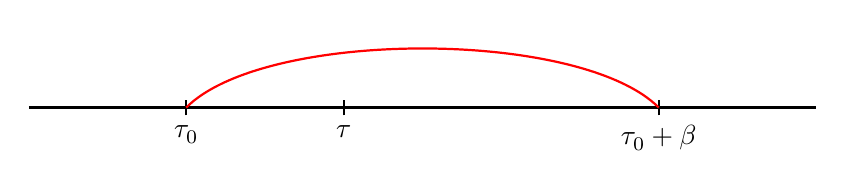
\begin{tikzpicture}
        \draw[thick] (-5,0) -- (5,0);
        \draw[thick] (-3,-0.1)node[below]{$\tau_0$} -- (-3,0.1);
        \draw[thick] (3,-0.1)node[below]{$\tau_0+\beta$} -- (3,0.1);
        \draw[thick] (-1,-0.1)node[below]{$\tau$} -- (-1,0.1);
        \draw[thick,red] (-3,0) .. controls (-2,1) and (2,1) .. (3,0);
    \end{tikzpicture}
\end{center}
\begin{equation}
    \begin{split}
        \mathcal{G}^T(\tau-\tau_0-\beta)&=\theta(\beta-\tau+\tau_0)\langle B(\tau_0)A(\tau-\beta)\rangle\\
        &=\frac{1}{Z}\sum_{n,m}e^{-\beta E_n}\langle n|B(\tau_0)|m\rangle\langle m|A(\tau_0)|n\rangle e^{(\tau-\beta-\tau_0)(E_m-E_n)}\\
        &=\frac{1}{Z}\sum_{n,m}e^{-\beta E_m}\langle n|B(\tau_0)|m\rangle\langle m|A(\tau_0)|n\rangle e^{(\tau-\tau_0)(E_m-E_n)}\\
        &=\mathcal{G}^T(\tau-\tau_0)
    \end{split}
\end{equation}
由于虚时格林函数的周期性,我们可以在范围$\tau_0<\tau<\tau_0+\beta$内进行傅里叶展开。傅里叶系数为
\begin{equation}
    \begin{split}
        \mathcal{G}^T(\omega_l)&=\int_{0}^{\beta}\mathrm{d}\tilde{\tau}e^{i\omega_l\tilde{\tau}}\mathcal{G}(\tilde{\tau})\\
        &=\int_{0}^{\beta}\mathrm{d}\tilde{\tau}e^{i\omega_l\tilde{\tau}}\theta(\tilde{\tau})\langle A(\tau)B(\tau_0)\rangle\\
        &=\frac{1}{Z}\int_{0}^{\beta}\mathrm{d}\tilde{\tau}e^{i\omega_l\tilde{\tau}}\sum_{n,m}e^{-\beta E_m}\langle n|B(\tau_0)|m\rangle\langle m|A(\tau_0)|n\rangle e^{\tilde{\tau}(E_m-E_n)}\\
        &=\frac{1}{Z}\sum_{n,m}\int_{0}^{\beta}\mathrm{d}\tilde{\tau}e^{(i\omega_l+E_m-E_n)\tilde{\tau}}e^{-\beta E_m}\langle n|B(\tau_0)|m\rangle\langle m|A(\tau_0)|n\rangle\\
        &=\frac{1}{Z}\sum_{n,m}\frac{e^{(i\omega_l+E_m-E_n)\beta}-1}{i\omega_l+E_m-E_n}e^{-\beta E_m}\langle n|B(\tau_0)|m\rangle\langle m|A(\tau_0)|n\rangle
    \end{split}
\end{equation}
值得注意玻色系统里$\omega_l=\frac{2\pi l}{\beta}$,所以$\beta\omega_l=2\pi l$
\begin{equation}
    \mathcal{G}^T(\omega_l)=\frac{1}{Z}\sum_{n,m}\frac{e^{-\beta E_n}-e^{-\beta E_m}}{i\omega_l+E_m-E_n}\langle n|B(\tau_0)|m\rangle\langle m|A(\tau_0)|n\rangle,\quad\omega_l=\frac{2\pi l}{\beta}
\end{equation}
上式可以写成积分形式
\begin{equation}
    \begin{split}
        \mathcal{G}^T(\omega_l)&=\frac{1}{Z}\int_{-\infty}^{+\infty}\mathrm{d}\omega'\sum_{n,m}\frac{e^{-\beta E_n}-e^{-\beta E_m}}{i\omega_l-\omega'}\langle n|B(\tau_0)|m\rangle\langle m|A(\tau_0)|n\rangle\delta(E_m-E_n+\omega')\\
        &=-\int_{-\infty}^{+\infty}\frac{\mathrm{d}\omega'}{2\pi}\frac{A_1(\omega')-A_2(\omega')}{i\omega_l-\omega'}\\
        &=-\int_{-\infty}^{+\infty}\frac{\mathrm{d}\omega'}{2\pi}\frac{A_1(\omega')}{i\omega_l-\omega}(1-e^{-\beta\omega'})
    \end{split}
\end{equation}
对比之前计算的实时推迟格林函数
\begin{equation}
    G^R(\omega)=\int_{-\infty}^{+\infty}\frac{\mathrm{d}\omega'}{2\pi}\frac{A_1(\omega')}{\omega-\omega'+i\eta}(1-e^{-\beta\omega'})
\end{equation}
可以看出,只需要将$-\mathcal{G}^T(i\omega_l)$做一个解析延拓$i\omega_l\rightarrow\omega+i\eta$即可得到实时推迟格林函数。这个解析延拓是非常奇怪的:$\mathcal{G}^T(\omega_l)$是只在虚轴的一系列离散点上有定义,但是我们可以从它得到定义在所有实轴上的实时推迟格林函数。
\subsubsection{电流-电流关联函数和电导}
我们现在准备用有限温度格林函数的形式将电导率在一阶线性响应中表示为电流-电流关联函数。电流的Kernel$D_{ij}(x-x',t-t')$包含了抗磁部分,这部分表达式为$ne\delta_{ij}\delta(x-x')\delta(t-t')$,这里我们忽略掉。注意,当我们通过皮尔斯替换得到紧束缚矩阵元的展开的流算符时,我们仅仅关注了$e^{i\int_{r_j}^{r_i}A\cdot dr}$的一阶展开;这也与忽略抗磁项对应。忽略抗磁项的原因不是因为它的贡献太小(抗磁项在计算超导体的电磁响应以及金属的响应修正上非常重要的。)然而这一项在时空里是对角项,因此对于霍尔电导或其他拓扑不变量没有贡献。

对电流的傅里叶变换
\begin{equation}
    J_i(k,\omega)=D_{ij}(k,\omega)A_j(k,\omega)=i\omega\sigma_{ij}(k,\omega)A_j(k,\omega)
\end{equation}
从之前的有限温度格林函数的阐述中,我们可以把推迟格林函数的计算转化为有限温度格林函数的计算。这个过程实际上也可以帮助我们获得有限温度的电导率。我们通过计算有限温度格林函数并作解析延拓后可以获得推迟格林函数。首先对位置坐标进行傅里叶变换;利用哈密顿量的平移不变性,从而得到格林函数
\begin{equation}
    \begin{split}
        \mathcal{G}_{ij}^T(x-x',\tau-\tau')=\langle T[j_i(x,\tau)j_j(x',\tau')]\rangle
    \end{split}
\end{equation}
$\tau>\tau'$时,对$x-x'$作傅里叶变换得到
\begin{equation}
    \begin{split}
        \mathcal{G}_{ij}^T(q,\tau-\tau')=\int_{-\infty}^{+\infty}\mathrm{d}(x-x')\langle j_i(x,\tau)j_j(x',\tau')\rangle e^{iq(x-x')}
    \end{split}
\end{equation}
利用$V\delta_{k+k'}=\int_{-\infty}^{+\infty}d(x+x')e^{i(k+k')(x+x')}$得到
\begin{equation}
    \begin{split}
        \mathcal{G}_{ij}^T(q,\tau-\tau')&=\frac{1}{V}\int_{-\infty}^{+\infty}\mathrm{d}(x+x')\mathrm{d}(x-x')\langle j_i(x,\tau)j_j(x',\tau')\rangle e^{iq(x-x')}\\
        &=\frac{1}{V}\int_{-\infty}^{+\infty}\mathrm{d}x\mathrm{d}x'\langle j_i(x,\tau)e^{iqx}j_j(x',\tau')e^{-iqx'}\rangle\\
        &=\langle j_i(q,\tau)j_j(-q,\tau')\rangle
    \end{split}
\end{equation}
同理对于$\tau<\tau'$
\begin{equation}
    \mathcal{G}_{ij}^T(q,\tau-\tau')=\langle j_j(-q,\tau')j_i(q,\tau)\rangle
\end{equation}
所以
\begin{equation}
    \mathcal{G}_{ij}^T(q,\tau-\tau')=\langle T[j_i(q,\tau)j_j(-q,\tau')]\rangle
\end{equation}
这里虚时流算符的定义为$j_i(q,\tau)=e^{\tau H}j_i(q)e^{-\tau H}$,我们有
\begin{equation}
    j_i(q,\tau)=\sum_{k}c_{k+\frac{q}{2},\alpha}^\dagger(\tau)\frac{\partial \epsilon^{\alpha\beta}(k)}{\partial k_i}c_{k-\frac{q}{2},\beta}(\tau)
\end{equation}
带入格林函数中得到
\begin{equation}
    \mathcal{G}^T_{ij}(q,\tau-\tau')=\sum_{k,p}\frac{\partial\epsilon^{\alpha\beta}(k)}{\partial k_i}\frac{\partial\epsilon^{\gamma\theta}(p)}{\partial p_j}\langle T[c_{k+\frac{q}{2},\alpha}^\dagger(\tau)c_{k-\frac{q}{2},\beta}(\tau)c_{p-\frac{q}{2},\gamma}^\dagger(\tau')c_{p+\frac{q}{2},\theta}(\tau')]\rangle
\end{equation}
利用Wick定理,
\begin{equation}
    \langle T[c_{k+\frac{q}{2},\alpha}^\dagger(\tau)c_{k-\frac{q}{2},\beta}(\tau)c_{p-\frac{q}{2},\gamma}^\dagger(\tau')c_{p+\frac{q}{2},\theta}(\tau')]\rangle=\langle Tc_{k+\frac{q}{2},\alpha}^\dagger(\tau)c_{p+\frac{q}{2},\theta}(\tau')\rangle\langle Tc_{k-\frac{q}{2},\beta}(\tau)c_{p-\frac{q}{2},\gamma}^\dagger(\tau')\rangle\delta_{\alpha\theta}\delta_{\beta\gamma}\delta_{kp}
\end{equation}
\begin{equation}
    \langle Tc_{k+\frac{q}{2},\alpha}^\dagger(\tau)c_{p+\frac{q}{2},\theta}(\tau')\rangle\delta_{kp}\delta_{\alpha\theta}=-\mathcal{G}_{\alpha\theta}^{(0))}(k+\frac{q}{2},\tau'-\tau)\delta_{kp}\delta_{\alpha\theta}
\end{equation}
\begin{equation}
    \langle Tc_{k-\frac{q}{2},\beta}(\tau)c_{p-\frac{q}{2},\gamma}^\dagger(\tau')\rangle\delta_{kp}\delta_{\beta\gamma}=-\mathcal{G}_{\beta\gamma}^{(0)}(k-\frac{q}{2},\tau-\tau')\delta_{kp}\delta_{\beta\gamma}
\end{equation}
值得注意这里$\mathcal{G}^{(0)}(k,\tau-\tau')$是费米算符的格林函数,满足$0<\tilde{\tau}<\beta$上的反周期关系:
\begin{equation}
    \mathcal{G}^{(0)}(k,\tilde{\tau})=-\mathcal{G}^{(0)}(k,\tilde{\tau}+\beta)
\end{equation}
对于费米算符格林函数而言有傅里叶变换
\begin{equation}
    \begin{cases}
        \mathcal{G}(k,\tau)&=\frac{1}{\beta}\sum_{n}e^{-i\omega_n\tau}\mathcal{G}(k,\omega_n)\\
        \mathcal{G}(k,\omega_n)&=\int_{0}^{\beta}\mathrm{d}\tau e^{i\omega_n\tau}\mathcal{G}(k,\tau)
    \end{cases}
\end{equation}
其中$\omega_n=\frac{(2n+1)\pi}{\beta}$,对于玻色算符的格林函数而言$\omega_n=\frac{2n\pi}{\beta}$

所以流-流虚时格林函数为
\begin{equation}
    \begin{split}
        \mathcal{G}^{T}_{ij}(q,\tau-\tau')&=-\sum_{k,p,\alpha,\beta,\gamma,\theta}\frac{\partial \epsilon^{\alpha\beta}(k)}{\partial k_i}\frac{\partial \epsilon^{\gamma\theta}(p)}{\partial p_j}\mathcal{G}_{\theta\alpha}^{(0)}(k+\frac{q}{2},\tau'-\tau)\mathcal{G}_{\beta\gamma}(k-\frac{q}{2},\tau-\tau')\delta_{kp}\delta_{\alpha\theta}\delta_{\beta\gamma}\\
        &=-\sum_{k,\alpha,\beta}\frac{\partial\epsilon^{\alpha\beta}(k)}{\partial k_i}\frac{\partial\epsilon^{\beta\alpha}(k)}{\partial k_j}\mathcal{G}_{\alpha\alpha}^{(0)}(k+\frac{q}{2},\tau'-\tau)\mathcal{G}_{\beta\beta}^{(0)}(k-\frac{q}{2},\tau-\tau')\\
        &=-\sum_{k,\alpha,\beta}\frac{\partial\epsilon^{\alpha\beta}(k)}{\partial k_i}\frac{\partial\epsilon^{\beta\alpha}(k)}{\partial k_j}\frac{1}{\beta}\sum_{m}e^{-i\omega_m(\tau'-\tau)}\mathcal{G}_{\alpha\alpha}^{(0)}(k+\frac{q}{2},\omega_m)\frac{1}{\beta}\sum_{n}e^{-i\omega_n(\tau-\tau')}\mathcal{G}_{\beta\beta}^{(0)}(k-\frac{q}{2},\omega_n)\\
        &=-\frac{1}{\beta^2}\sum_{k,m,n,\alpha,\beta}\frac{\partial\epsilon^{\alpha\beta}(k)}{\partial k_i}\frac{\partial\epsilon^{\beta\alpha}(k)}{\partial k_j}\mathcal{G}_{\alpha\alpha}^{(0)}(k+\frac{q}{2},\omega_m)\mathcal{G}_{\beta\beta}^{(0)}(k-\frac{q}{2},\omega_n)e^{i(\omega_m-\omega_n)(\tau-\tau')}
    \end{split}
\end{equation}
对上式做傅里叶变换得到
\begin{equation}
    \begin{split}
        \mathcal{G}_{ij}^T(q,\nu_r)&=\int_{0}^{\beta}\mathrm{d}(\tau-\tau')e^{i\nu_r(t-t')}\mathcal{G}_{ij}^T(q,\tau-\tau')\\
        &=-\frac{1}{\beta^2}\int_{0}^{\beta}\mathrm{d}(\tau-\tau')e^{i\nu_r(t-t')}\sum_{k,m,n,\alpha,\beta}\frac{\partial\epsilon^{\alpha\beta}(k)}{\partial k_i}\frac{\partial\epsilon^{\beta\alpha}(k)}{\partial k_j}\mathcal{G}_{\alpha\alpha}^{(0)}(k+\frac{q}{2},\omega_m)\mathcal{G}_{\beta\beta}^{(0)}(k-\frac{q}{2},\omega_n)e^{i(\omega_m-\omega_n)(\tau-\tau')}\\
        &=-\frac{1}{\beta^2}\sum_{k,m,n,\alpha,\beta}\int_{0}^{\beta}\mathrm{d}(\tau-\tau')e^{i(\omega_m-\omega_n+\nu_r)(\tau-\tau')}\frac{\partial\epsilon^{\alpha\beta}(k)}{\partial k_i}\frac{\partial\epsilon^{\beta\alpha}(k)}{\partial k_j}\mathcal{G}_{\alpha\alpha}^{(0)}(k+\frac{q}{2},\omega_m)\mathcal{G}_{\beta\beta}^{(0)}(k-\frac{q}{2},\omega_n)
    \end{split}
\end{equation}
这里$\omega_m=\frac{(2m+1)\pi}{\beta},\omega_n=\frac{(2n+1)\pi}{\beta},\nu_r=\frac{2r\pi}{\beta}$,所以
\begin{equation}
    \begin{split}
        \int_0^\beta\mathrm{d}(\tau-\tau')e^{i(\omega_m-\omega_n+\nu_r)(\tau-\tau')}&=\frac{e^{i(\omega_m-\omega)n+\nu_r)\beta}-1}{i(\omega_m-\omega_n+\nu_r)}\\
        &=\frac{e^{i2pi(m-n+r)}-1}{i\frac{2\pi}{\beta}(m-n+r)}\\
        &=\beta\delta_{m-n+r}=\beta\delta_{\omega_m-\omega_n+\nu_r}
    \end{split}
\end{equation}
所以得到
\begin{equation}
    \mathcal{G}_{ij}^T(q,\nu_r)=-\frac{1}{\beta}\sum_{n,k}Tr\left[\frac{\epsilon(k)}{\partial k_i}\mathcal{G}^{(0)}(k-\frac{q}{2},\omega_n)\frac{\epsilon(k)}{\partial k_j}\mathcal{G}^{(0)}(k+\frac{q}{2},\omega_n-\nu_r)\right]
\end{equation}
或者
\begin{equation}
    \mathcal{G}_{ij}^T(q,\nu_r)=-\frac{1}{\beta}\sum_{m,k}Tr\left[\frac{\epsilon(k)}{\partial k_i}\mathcal{G}^{(0)}(k-\frac{q}{2},\omega_m+\nu_r)\frac{\epsilon(k)}{\partial k_j}\mathcal{G}^{(0)}(k+\frac{q}{2},\omega_m)\right]
\end{equation}
正如之前所说,我们只需要对$-\mathcal{G}^{T}(\omega_n)$做一个解析延拓$i\omega_n\rightarrow\omega+i\eta$即可得到响应函数$D(\omega)$。最后只需要利用Kubo定理计算电导张量即可
\begin{equation}
    i\omega\sigma_{ij}(q,\omega)=D_{ij}(q,\omega)
\end{equation}
\subsubsection{霍尔电导的计算}
我们现在已经可以用之前已经建立的工具来计算绝缘体的霍尔电导。我们试着一举两得:我们试着计算霍尔电导和引入绝缘体哈密顿量的极限——平带极限。在这个极限下的哈密顿量与原来的哈密顿量是拓扑等价的,并且将在书中被反复使用来进行简单计算关联函数和纠缠谱。对于任意带数的一般情况,电导率公式是非常繁琐的:其中出现的格林函数在所有能带能量都包含极点,而这些能带能量通常是不同的。计算是繁琐的,因为我们必须考虑所有极点的留数。平带极限所实现的是将哈密顿函数的所有占据的能量放在$-E$,而所有未占据的状态放在能量$+E$(按照惯例,$E$在某些能量单位中通常被选择为$1$),同时保持系统的本征态不变。系统的拓扑性质不应该依赖于占据能带的能量:平带极限将会证明这点。我们最终所发现的是霍尔电导并不依赖能带的能量——它仅仅依赖本征态。这是霍尔电导的拓扑性质的第一个实际线索。哈密顿绝热演化过程中,如果我们发现霍尔电导依赖于占据带的能量,那么他将不会是拓扑不变的:通过对哈密顿做一个小的绝热变换(不会关闭能隙),我们将会获得不同的霍尔电导。实际上,我们可以证明这不是真实的,这是霍尔电导是一个真正拓扑量的线索。

哈密顿量$H=\sum_{k,\alpha,\beta}c_{k,\alpha}\epsilon^{\alpha\beta}(k)c_{k,\beta}$很容易通过把矩阵$(\epsilon(k))_{\alpha\beta}=\epsilon^{\alpha\beta}(k)$对角化来求解。这个解给出了哈密顿的能带。
\begin{equation}
    \epsilon^{\alpha\beta}(k)u_{\beta}^{i}(k)=\epsilon_{i}(k)u_{\alpha}^{i}(k)
\end{equation}
其中$u_{\alpha}^{i}(k)$是矢量$u^i(k)$的第$\alpha$分量,这是在动量$k$时哈密顿的对应于能量$\epsilon_i(k)$的第$i$个单粒子本征态。我们可以对角化能量矩阵
\begin{equation}
    U^\dagger\epsilon(k)U=\begin{pmatrix}
        \epsilon_1(k)&\quad&\quad\\
        \quad&\cdots&\quad\\
        \quad&\quad&\epsilon_{m}(k)
    \end{pmatrix}=\tilde{\epsilon}(k)
\end{equation}
系统有$m$个轨道(子格自由度、自旋自由度等)。这里$\tilde{\epsilon}(k)$是系统的能量矩阵——单粒子对角化能量矩阵。变换矩阵元$U_{\alpha i}=u_\alpha^i$,满足幺正性,因为不同能级的本征向量相互正交
\begin{equation}
    U^\dagger U=(U^\dagger)_{i\alpha}U_{\alpha j}=U_{\alpha i}^*U_{\alpha j}=u_\alpha^{*i}u_{\alpha}^{j}=\delta_{ij}
\end{equation}
利用幺正变换可以把二次型哈密顿量对角化
\begin{equation}
    \begin{split}
        H&=\sum_{k}c_{\alpha}^\dagger(k)\epsilon^{\alpha\beta}(k)c_\beta(k)\\
        &=\sum_{k}c_{\alpha}^\dagger(k)U_{\alpha i}U_{i\alpha}^\dagger\epsilon^{\alpha\beta}(k)U_{\beta j}U_{j\beta}^\dagger c_\beta(k)\\
        &=\sum_{k}\gamma_i^\dagger(k)\epsilon_i(k)\delta_{ij}\gamma_j(k)\\
        &=\sum_{k}\gamma_i^\dagger(k)\epsilon_i(k)\gamma_i(k)
    \end{split}
\end{equation}
其中
\begin{equation}
    \gamma_i(k)=U_{i\alpha}^\dagger c_{\alpha}(k)
\end{equation}
幺正变换$U$现在允许我们做一个绝热变换来帮助我们求解一般系统的霍尔电导
\subsubsection{哈密顿对角化以及平带基}
假设系统是绝缘体,我们可以把费米能级放在绝缘体能隙中或者说把满带放在零能以下,所以我们填满了所有的负能带(以费米面为能量零点)。对于一个p满带的绝缘体,我们假设能级之间有如下不等式
\begin{equation}
    \epsilon_1(k)\leq\epsilon_2(k)\leq\cdots\leq\epsilon_p(k)\leq\epsilon_{p+1}(k)\leq\cdots\leq\epsilon_m(k)
\end{equation}
我们选择两个任意的能量$\epsilon_G$和$\epsilon_E$,有约束条件$\epsilon_G<0<\epsilon_E$,$G,E$分别是占据基态和空态。$\epsilon_G,\epsilon_E$可以为常数,例如$\pm 1eV$. 我们现在引入$\epsilon_1,\cdots,\epsilon_p$到$\epsilon_G$和$\epsilon_{p+1},\cdots,\epsilon_m$到$\epsilon_E$的绝热内插
\begin{equation}
    \begin{split}
        E_i(k,t)&=\epsilon_i(k)(1-t)+\epsilon_Gt,\quad 1\leq i\leq p\\
        E_i(k,t)&=\epsilon_i(k)(1-t)+\epsilon_Et,\quad p+1\leq i\leq m
    \end{split}
\end{equation}
哈密顿在绝热演化中能隙始终是打开的,没有能带穿越费米能级,更进一步说,能带的结构在绝热演化过程中始终是相同的。最后一步实际上并不重要;唯一重要的性质是哈密顿对于任意的绝热参数$t\in[0,1]$能隙都是打开的。因为费米能级处于能隙中,并且没有任何态在绝热演化中穿过费米能级。我们立即可以意识到这个内插哈密顿的拓扑性质和原始哈密顿是相同的。这个结果实际上可以通过证明霍尔电导不依赖内插能量$E_i(k,t)$来证实。我们考虑的内插哈密顿为
\begin{equation}
    H(k,t)=U(k)\begin{pmatrix}
        E_1(k,t)&\quad&\quad&\quad&\quad&\quad\\
        \quad&\cdots&\quad&\quad&\quad&\quad\\
        \quad&\quad&E_p(k,t)&\quad&\quad&\quad\\
        \quad&\quad&\quad&E_{p+1}(k,t)&\quad&\quad\\
        \quad&\quad&\quad&\quad&\cdots&\quad\\
        \quad&\quad&\quad&\quad&\quad&E_m(k,t)
    \end{pmatrix}U^\dagger(k)
\end{equation}
这个内插哈密顿介于原系统和$t=1$的平带系统之间。$t=1$时,哈密顿有一个非常好的性质,此时的哈密顿是系数为$\epsilon_G$的各个占据态的投影算符之和与系数为$\epsilon_E$的各个空态之和的叠加
\begin{equation}
    H(k,1)=\epsilon_G\sum_{\alpha=1}^p|\alpha,k\rangle\langle \alpha,k|+\epsilon_E\sum_{\beta=p+1}^m|\beta,k\rangle\langle\beta,k|
\end{equation}
这里稍微写一下上式计算。我们定义矢量$|i,k\rangle=\begin{pmatrix}u_1^i(k)\\\cdots\\u_m^i(k)\end{pmatrix}$,所以
\begin{equation}
    U(k)=\begin{bmatrix}
        u_1^1(k)&u_1^2(k)&\cdots&u_1^m(k)\\
        u_2^1(k)&u_2^2(k)&\cdots&u_2^m(k)\\
        \cdots&\cdots&\cdots&\cdots\\
        u_m^1(k)&u_m^2(k)&\cdots&u_m^m(k)
    \end{bmatrix}=(|1,k\rangle,|2,k\rangle,\cdots,|m,k\rangle)
\end{equation}
所以
\begin{equation}
    \begin{split}
        U(k)H(k,t)U^\dagger(k)&=(|1,k\rangle,|2,k\rangle,\cdots,|m,k\rangle)\begin{pmatrix}
            E_1(k,t)&\quad&\quad&\quad&\quad&\quad\\
        \quad&\cdots&\quad&\quad&\quad&\quad\\
        \quad&\quad&E_p(k,t)&\quad&\quad&\quad\\
        \quad&\quad&\quad&E_{p+1}(k,t)&\quad&\quad\\
        \quad&\quad&\quad&\quad&\cdots&\quad\\
        \quad&\quad&\quad&\quad&\quad&E_m(k,t)
        \end{pmatrix}\begin{pmatrix}
            \langle 1,k|\\
            \langle 2,k|\\
            \cdots\\
            \langle m,k|
        \end{pmatrix}\\
        &=(|1,k\rangle,|2,k\rangle,\cdots,|m,k\rangle)\begin{pmatrix}
            E_1(k,t)\langle 1,k|\\
            E_2(k,t)\langle 2,k|\\
            \cdots\\
            E_m(k,t)\langle m,k|
        \end{pmatrix}\\
        &=\sum_{\alpha}E_\alpha(k,t)|\alpha,k\rangle\langle\alpha,k|
    \end{split}
\end{equation}
对于$t=1$的情况,
\begin{equation}
    H(k,1)=\epsilon_G\sum_{i=1}^p|i,k\rangle\langle i,k|+\epsilon_E\sum_{i=p+1}^m|i,k\rangle\langle i,k|
\end{equation}
得证

其中$|i,k\rangle\langle i,k|=u_n^i(k)u_m^{i*}(k)=\mathcal{P}_{nm}^i$是$m,n$矩阵元,也是投影算符
\begin{equation}
    \mathcal{P}^iu^j=\mathcal{P}_{nm}^iu_m^i=u_n^iu_m^iu_m^j=u_n^i\delta_{ij}=u^j\delta_{ij}
\end{equation}
定义幂等元(投影算符)
\begin{equation}
    \begin{split}
        P_G&=\sum_{i=1}^{p}|i,k\rangle\langle i,k|=\sum_{i=1}^{p}u_n^i(k)u_m^{i*}(k)=\sum_{i=1}^{p}\mathcal{P}_{nm}^i\\
        P_E&=\sum_{i=p+1}^{m}|i,k\rangle\langle i,k|=\sum_{i=p+1}^{m}u_n^i(k)u_m^{i*}(k)=\sum_{i=p+1}^{m}\mathcal{P}_{nm}^i
    \end{split}
\end{equation}
很显然
\begin{equation}
    P_G^2=\sum_{i,j=1}^{p}u_n^i(k)u_m^{i*}(k)u_m^{j}(k)u_s^{j*}(k)=\sum_{i=1}^{p}u_n^i(k)u_s^{i*}(k)=P_G
\end{equation}
\begin{equation}
    P_E^2=\sum_{i,j=p+1}^{m}u_n^i(k)u_m^{i*}(k)u_m^{j}(k)u_s^{j*}(k)=\sum_{i=p+1}^{m}u_n^i(k)u_s^{i*}(k)=P_E
\end{equation}
\begin{equation}
    P_EP_G=\sum_{i=1}^{p}\sum_{j=p+1}^{m}u_n^i(k)u_m^{i*}(k)u_m^{j}u_s^{j*}(k)=\sum_{i=1}^{p}\sum_{j=p+1}^{m}u_n^i(k)\delta_{ij}u_m^j(k)=0
\end{equation}
$P_G,P_E$相互正交,生成互补子空间$\mathcal{L}_G$和$\mathcal{L}_E$. 
\begin{equation}
    H(k,1)=\epsilon_GP_G+\epsilon_EP_E
\end{equation}
平带方法的好处在于可以把系统的格林函数写成非常简单的形式
\begin{equation}
    \mathcal{G}(i\omega_m,k)=\frac{P_G(k)}{i\omega_m-\epsilon_G}+\frac{P_E(k)}{i\omega_m-\epsilon_E}
\end{equation}
上式很容易证明,我们只需要计算
\begin{equation}
    \begin{split}
        &(i\omega_m-\epsilon_GP_G-\epsilon_EP_E)(\frac{P_G}{i\omega_m-\epsilon_G}+\frac{P_E}{i\omega_m-\epsilon_E})=\frac{i\omega_mP_G-\epsilon_GP_G}{i\omega_m-\epsilon_G}+\frac{i\omega_mP_E-\epsilon_EP_E}{i\omega_m-\epsilon_E}\\
        &=\frac{-\omega_m^2P_G-i\omega\epsilon_EP_G-i\omega_m\epsilon_GP_G-\epsilon_G\epsilon_EP_G-\omega_m^2P_E-i\omega_mP_E\epsilon_G-i\omega_m\epsilon_EP_E+\epsilon_E\epsilon_GP_E}{-\omega_m^2-i\omega_m\epsilon_E-i\omega_m\epsilon_G}\\
        &=1
    \end{split}
\end{equation}
所以可以得到
\begin{equation}
    \begin{split}
        \mathcal{G}(i\omega_m,k)&=\frac{1}{i\omega_m-H(k,1)}\\
        &=\frac{1}{i\omega_m-\epsilon_GP_G-\epsilon_EP_E}\\
        &=\frac{P_G(k)}{i\omega_m-\epsilon_G}+\frac{P_E}{i\omega_m-\epsilon_E}
    \end{split}
\end{equation}
显然绝热哈密顿的流为
\begin{equation}
    \frac{\partial H(k,1)}{\partial k_i}=\epsilon_G\frac{\partial P_G(k)}{\partial k_i}+\epsilon_E\frac{\partial P_E(k)}{\partial k_i}=(\epsilon_G-\epsilon_E)\frac{\partial P_G(k)}{\partial k_i}
\end{equation}
最后一步利用了$P_G+P_E=1$,两边同时对$k_i$求导即可得到。所以平带极限下有限温度格林函数可以写成
\begin{equation}
    \begin{split}
        \mathcal{G}_{ij}^T(q,\nu_r)&=-\frac{1}{\beta}\sum_{m,k}Tr\left[\frac{\partial H(k,1)}{\partial k_i}\mathcal{G}^{(0)}(k-\frac{q}{2},\omega_m+\nu_r)\frac{\partial H(k,1)}{\partial k_j}\mathcal{G}^{(0)}(k+\frac{q}{2},\omega_m)\right]\\
        &=-\frac{1}{\beta}\sum_{m,k}(\epsilon_G-\epsilon_E)^2Tr\left[\frac{\partial P_G(k)}{\partial k_i}(\frac{P_G(k-\frac{q}{2})}{i(\omega_m+\nu_r)-\epsilon_G}+\frac{P_E(k-\frac{q}{2})}{i(\omega+\nu_r)-\epsilon_E})\frac{\partial P_G(k)}{\partial k_j}(\frac{P_G(k+\frac{q}{2})}{i\omega_m-\epsilon_G}+\frac{P_E(k+\frac{q}{2})}{i\omega_m-\epsilon_E})\right]\\
    \end{split}
\end{equation}
考虑直流的情况$q\to0$
\begin{equation}
    \mathcal{G}_{ij}^T(\nu_r)=-\frac{1}{\beta}\sum_{m,k}Tr\left[\frac{\partial P_G(k)}{\partial k_i}(\frac{P_G(k)}{i(\omega_m+\nu_r)-\epsilon_G}+\frac{P_E(k)}{i(\omega_m+\nu_r)-\epsilon_E})\frac{\partial P_G(k)}{\partial k_j}(\frac{P_G(k)}{i\omega_m-\epsilon_G}+\frac{P_E(k)}{i\omega_m-\epsilon_E})\right]
\end{equation}
值得注意,投影算符之间有如下代数关系
\begin{equation}
    P_{G}\left(\partial_{i} P_{G}\right)=\partial_{i} P_{G}-\left(\partial_{i} P_{G}\right) P_{G}, \quad\left(\partial_{i} P_{E}\right) P_{G}=-P_{E} \partial_{i} P_{G}, \quad \partial_{i} P_{G}=-\partial_{i} P_{E}
\end{equation}
\begin{equation}
    \left(\partial_{i} P_{G}\right) P_{G}\left(\partial_{j} P_{G}\right) P_{G}=\left(\partial_{i} P_{G}\right)\left(\partial_{j} P_{G}\right) P_{G}-\left(\partial_{i} P_{G}\right)\left(\partial_{j} P_{G}\right) P_{G}^{2}=0
\end{equation}
上面三式对于$E\rightarrow E$也成立。由上面三式可以得到格林函数中的四项投影算符
\begin{equation}
    \begin{split}
        &\left(\partial_{i} P_{G}\right) P_{G}\left(\partial_{j} P_{E}\right) P_{G}=-\left(\partial_{i} P_{G}\right)\left(\partial_{j} P_{G}\right) P_{E} P_{G}=0\\
        &\left(\partial_{i} P_{G}\right) P_{E}\left(\partial_{j} P_{G}\right) P_{E}=-\left(\partial_{i} P_{G}\right)\left(\partial_{j} P_{E}\right) P_{G} P_{E}=0\\
        &\left(\partial_{i} P_{G}\right) P_{G}\left(\partial_{j} P_{G}\right) P_{E}=-\left(\partial_{i} P_{G}\right) P_{G}\left(\partial_{j} P_{E}\right) P_{E}=\left(\partial_{i} P_{G}\right)\left(\partial_{j} P_{G}\right) P_{E}^{2}=-\left(\partial_{i} P_{G}\right)\left(\partial_{j} P_{E}\right) P_{E}\\
        &\left(\partial_{i} P_{G}\right) P_{E}\left(\partial_{j} P_{G}\right) P_{G}=-\left(\partial_{i} P_{G}\right)\left(\partial_{j} P_{E}\right) P_{G}
    \end{split}
\end{equation}
所以最后有限温度流——流格林函数为
\begin{equation}
    \mathcal{G}_{ij}^T(q,\nu_r)=-\frac{1}{\beta}\sum_{m,k}(\epsilon_G-\epsilon_E)^2Tr\left[\frac{\partial P_G}{\partial k_i}\frac{P_G}{i(\omega_m+\nu_r)-\epsilon_G}\frac{\partial P_G}{\partial k_j}\frac{P_E}{i\omega_m-\epsilon_E}+\frac{\partial P_G}{\partial k_i}\frac{P_E}{i(\omega_m+\nu_r)-\epsilon_E}\frac{\partial P_G}{\partial k_j}\frac{P_G}{i\omega_m-\epsilon_G}\right]
\end{equation}
对$\omega_m=i\frac{2m\pi}{\beta}$求和需要利用松原求和方法。我们分为两项计算

对于第一项
\begin{equation}
    \frac{1}{\beta}\sum_{m}\frac{(\partial_i P_G)P_G(\partial_j P_G)P_E}{(i\omega_m-\epsilon_G+i\nu_r)(i\omega_m-\epsilon_E)}=\frac{1}{\beta}\sum_{m}f(i\omega_m)
\end{equation}
求和思路是构造一个单极点为$i\omega_m$的辅助函数,利用留数定理得到求和表达式。对于费米系统来说,$i\omega_m=i\frac{(2m+1)\pi}{\beta}$正好是费米占据函数$n_F=\frac{1}{e^{\beta z+1}}$的单极点,留数为$-\frac{1}{\beta}$. 所以我们构造积分
\begin{equation}
    I=\oint\frac{\mathrm{d}z}{2\pi i}f(z)n_F(z)
\end{equation}
这个积分的留数如下
\begin{equation}
    \begin{split}
        z_1&=\epsilon_G-i\nu_r,\quad res[f(z_1)n_F(z_1)]=\frac{(\partial_iP_G)P_G(\partial_JP_G)P_E}{\epsilon_G-\epsilon_E-i\nu_r}n_F(\epsilon_G-i\nu_r)=\frac{(\partial_iP_G)P_G(\partial_JP_G)P_E}{\epsilon_G-\epsilon_E-i\nu_r}n_F(\epsilon_G)\\
        z_2&=\epsilon_E,\quad res[f(z_2)n_F(z_2)]=\frac{(\partial_iP_G)P_G(\partial_JP_G)P_E}{\epsilon_E-\epsilon_G+i\nu_r}n_F(\epsilon_E)\\
        z_m&=i\omega_m,\quad res[f(z_m)n_F(z_m)]-\frac{1}{\beta}f(i\omega_m)
    \end{split}
\end{equation}
\begin{center}
    \begin{tikzpicture}
        \draw[->] (-3,0) -- (3,0) node[below=1em,right]{$x$};
        \draw[->] (0,-3) -- (0,3) node[above=1em,right]{$y$};
        \node[below=1em,left] at (0,0) {$O$};
        \node at (0,0.5) {$\times$};
        \node at (0,1.5) {$\times$};
        \node at (0,2.5) {$\times$};
        \node[right] at (0,2.5) {$i\omega_m$};
        \node at (0,-0.5) {$\times$};
        \node at (0,-1.5) {$\times$};
        \node at (0,-2.5) {$\times$};
        \node at (2,0) {$\times$};
        \node[below] at (2,0) {$\epsilon_E$};
        \node at (-2,-1) {$\times$};
        \node[above] at (-2,-1) {$\epsilon_G-i\nu_r$};
        \draw (0,0) circle (2.8);
    \end{tikzpicture}
\end{center}
取上图所示的围道,并且令$R\to+\infty$得到
\begin{equation}
    \lim_{R\to+\infty}\oint\frac{\mathrm{d}z}{2\pi i}f(z)n_F(z)=0
\end{equation}
由留数定理可知
\begin{equation}
    -\frac{1}{\beta}\sum_mf(i\omega_m)+\frac{(\partial_iP_G)P_G(\partial_jP_G)P_E}{\epsilon_G-\epsilon_E-i\nu_r}n_F(\epsilon_G)+\frac{(\partial_iP_G)P_G(\partial_jP_G)P_E}{\epsilon_E-\epsilon_G+i\nu_r}n_F(\epsilon_E)=0
\end{equation}
所以得到
\begin{equation}
    \frac{1}{\beta}\sum_mf(i\omega_m)=\frac{(\partial_iP_G)P_G(\partial_jP_G)P_E}{\epsilon_G-\epsilon_E-i\nu_r}n_F(\epsilon_G)+\frac{(\partial_iP_G)P_G(\partial_jP_G)P_E}{\epsilon_E-\epsilon_G+i\nu_r}n_F(\epsilon_E)
\end{equation}
同理,对于第二项
\begin{equation}
    \frac{1}{\beta}\sum_{m}\frac{(\partial_i P_G)P_E(\partial_j P_G)P_G}{(i\omega_m-\epsilon_E+i\nu_r)(i\omega_m-\epsilon_G)}=\frac{1}{\beta}\sum_{m}f(i\omega_m)
\end{equation}
与第一项比较可知,只需要分子不变,分母和占据函数做替换$E\leftrightarrow G$即可得到
\begin{equation}
    \frac{1}{\beta}\sum_{m}f(i\omega_m)=\frac{(\partial_iP_G)P_E(\partial_jP_G)P_G}{\epsilon_E-\epsilon_G-i\nu_r}n_F(\epsilon_E)+\frac{(\partial_iP_G)P_E(\partial_jP_G)P_G}{\epsilon_G-\epsilon_E+i\nu_r}n_F(\epsilon_G)
\end{equation}
计算可知松原格林函数为
\begin{equation}
    \begin{split}
        \mathcal{G}_{ij}^T(i\nu_r)=-\sum_{k}(\epsilon_G-\epsilon_E)^2Tr\left[\frac{(\partial_iP_G)P_G(\partial_jP_G)P_E}{\epsilon_G-\epsilon_E-i\nu_r}n_F(\epsilon_G)+\frac{(\partial_iP_G)P_G(\partial_jP_G)P_E}{\epsilon_E-\epsilon_G+i\nu_r}n_F(\epsilon_E)\right.\\
        \left.+\frac{(\partial_iP_G)P_E(\partial_jP_G)P_G}{\epsilon_E-\epsilon_G-i\nu_r}n_F(\epsilon_E)+\frac{(\partial_iP_G)P_E(\partial_jP_G)P_G}{\epsilon_G-\epsilon_E+i\nu_r}n_F(\epsilon_G)\right]
    \end{split}
\end{equation}
对于零温的情况,占据态$\epsilon_E>0$的占据数$n_F(\epsilon_E)=0$,只有费米面以下的$\epsilon_G<0$是占满的$n_F(\epsilon_F)=1$. 所以我们可以得到零温时的松原格林函数
\begin{equation}
    \mathcal{G}_{ij}^T(i\nu_r)=-\sum_{k}(\epsilon_G-\epsilon_E)^2Tr\left[\frac{(\partial_iP_G)P_G(\partial_jP_G)P_E}{\epsilon_G-\epsilon_E-i\nu_r}+\frac{(\partial_iP_G)P_E(\partial_jP_G)P_G}{\epsilon_G-\epsilon_E+i\nu_r}\right]
\end{equation}
利用$(\partial_iP_G)P_G(\partial_jP_G)P_E=-(\partial_iP_G)(\partial_jP_E)P_E$和$(\partial_iP_G)P_E(\partial_jP_G)P_G=-(\partial_iP_G)(\partial_jP_E)P_G$
可以将上式化简为
\begin{equation}
    \mathcal{G}_{ij}^T(i\nu_r)=\sum_{k}(\epsilon_G-\epsilon_E)^2Tr\left[\frac{(\partial_iP_G)(\partial_jP_E)P_E}{\epsilon_G-\epsilon_E-i\nu_r}+\frac{(\partial_iP_G)(\partial_jP_E)P_G}{\epsilon_G-\epsilon_E+i\nu_r}\right]
\end{equation}
上式通分后舍去对称项,因为我们所计算的霍尔电导是电导张量的反对称分量
\begin{equation}
    \begin{split}
        \mathcal{G}_{ij}^T(i\nu_r)=\sum_{k}(\epsilon_G-\epsilon_E)^2Tr\left[\frac{(\epsilon_G-\epsilon_E)[(\partial_i P_G)(\partial_j P_E)P_E+(\partial_i P_G)(\partial_j P_E)P_G]}{(\epsilon_G-\epsilon_G)^2-(i\nu_r)^2}\right.\\
        \left.+\frac{i\nu_r[(\partial_i P_G)(\partial_j P_E)P_E-(\partial_i P_G)(\partial_j P_E)P_G]}{(\epsilon_G-\epsilon_E)^2-(i\nu_r)^2}\right]
    \end{split}
\end{equation}
可以看到上式第一项是对称项,交换指标$i\leftrightarrow j$后保持不变,所以舍去,我们关注第二项
\begin{equation}
    \mathcal{G}_{ij}^T(i\nu_r)=\sum_{k}(\epsilon_G-\epsilon_E)^2Tr\left[\frac{i\nu_r[(\partial_i P_G)(\partial_j P_E)P_E-(\partial_i P_G)(\partial_j P_E)P_G]}{(\epsilon_G-\epsilon_E)^2-(i\nu_r)^2}\right]
\end{equation}
计算$Tr[(\partial_i P_G)(\partial_j P_E)P_G]$
\begin{equation}
    \begin{split}
        Tr[(\partial_i P_G)(\partial_j P_E)P_G]&=Tr[P_G(\partial_i P_G)(\partial_j P_E)]\\
        &=-Tr[P_G(\partial_i P_E)(\partial_j P_E)]\\
        &=Tr[(\partial_i P_G)P_E(\partial_j P_E)]\\
        &=Tr[(\partial_i P_G)(\partial_j P_E)-(\partial_i P_G)(\partial_j P_E)P_E]\\
        &=-Tr[(\partial_i P_G)(\partial_j P_E)P_E]
    \end{split}
\end{equation}
这里最后一步利用了$Tr[(\partial_i P_G)(\partial_j P_E)]=-Tr[(\partial_i P_G)(\partial_j P_G)]=-Tr[(\partial_j P_G)(\partial_i P_G)]=Tr[(\partial_j P_G)(\partial_i P_E)]$是一个对称项,所以舍去了。带入反对称格林函数得到
\begin{equation}
    \mathcal{G}_{ij}^T(i\nu_r)=\sum_{k}(\epsilon_G-\epsilon_E)^2Tr\left[(\partial_i P_G)(\partial_j P_E)P_E\frac{2i\nu_r}{(\epsilon_G-\epsilon_E)^2-(i\nu_r)^2}\right]
\end{equation}
做一个解析延拓$i\nu_r\rightarrow\omega+i\eta$可以获得推迟格林函数(响应函数)
\begin{equation}
    G_{ij}^R(\omega)=-\sum_{k}(\epsilon_G-\epsilon_E)^2Tr\left[(\partial_i P_G)(\partial_j P_E)P_E\frac{2\omega}{(\epsilon_G-\epsilon_E)^2-(\omega+i\eta)^2}\right]
\end{equation}
在直流极限下$\omega\to 0$
\begin{equation}
    G_{ij}^R(\omega\to 0)=-2\omega\sum_{k}Tr[(\partial_i P_G)(\partial_j P_E)P_E]
\end{equation}
现在我们计算一下
\begin{equation}
    \begin{split}
        Tr[(\partial_i P_G)(\partial_j P_E)P_E]&=Tr[(\partial_iP_G)(\partial_jP_E)]-Tr[(\partial_iP_G)P_E(\partial_jP_E)]\\
        &=-Tr[\partial_i P_G\partial_j P_G]+Tr[P_G(\partial_iP_E)(\partial_jP_E)]\\
        &=-Tr[(\partial_iP_G)(\partial_jP_G)]+Tr[(\partial_iP_G)(\partial_jP_G)P_G]
    \end{split}
\end{equation}
由于$Tr[AB]=Tr[BA]$, 第一项是对称项,我们舍去这一项。我们现在得到了完全用占据带基态投影算符$P_G(k)$表示的关联函数。数值上,这是我们计算霍尔电导的方法,因为投影算符是规范不变的,绕过了需要光滑规范的要求。我们把它表示成布洛赫态的显式表示
\begin{equation}
    \begin{split}
        &Tr[(\partial_iP_G)(\partial_jP_G)P_G]=\sum_{\alpha,\alpha',\alpha'',\beta}\left[\langle\beta,k|(|\partial_i\alpha,k\rangle\langle\alpha,k|+|\alpha,k\rangle\langle\partial_i\alpha,k|)(|\partial_j\alpha',k\rangle\langle\alpha',k|\right.\\
        &\left.+|\alpha',k\rangle\langle\partial_j\alpha',k|)|\alpha'',k\rangle\langle\alpha'',k|\beta,k\rangle\right]\\
        &=\sum_{\alpha,\alpha',\beta}\left[\langle\beta,k|(|\partial_i\alpha,k\rangle\langle\alpha,k|+|\alpha,k\rangle\langle\partial_i\alpha,k|)(|\partial_j\alpha',k\rangle\langle\alpha',k|+|\alpha',k\rangle\langle\partial_j\alpha',k|)|\beta,k\rangle\right]\\
        &=\sum_{\alpha,\beta}\langle\beta,k|\partial_i\alpha,k\rangle\langle\alpha,k|\partial_j\beta,k\rangle+\sum_{\alpha,\beta}\langle\beta,k|\partial_i\alpha,k\rangle\langle\partial_j\alpha,k|\beta,k\rangle+\sum_{\alpha}\langle\partial_i\alpha,k|\partial_j\alpha,k\rangle+\sum_{\alpha,\alpha'}\langle\partial_i\alpha,k|\alpha',k\rangle\langle\partial_j\alpha',k|\alpha,k\rangle
    \end{split}
\end{equation}
只有第三项是关于指标$i,j$的反对称项,其余几项总可以通过交换$i\leftrightarrow j$变回原来的形式。
\begin{equation}
    \epsilon_{ij}Tr[(\partial_iP_G)(\partial_jP_G)P_G]=\sum_{\alpha}[\langle\partial_i\alpha,k|\partial_j\alpha,k\rangle-\langle\partial_j\alpha,k|\partial_i\alpha,k\rangle]
\end{equation}
显式表达式推导的过程中,布洛赫函数可微,这暗示了BZ上的规范必须是光滑规范。这通常是一个相当复杂的过程,这就是为什么我们用投影算符表示关联函数的形式。因此我们可以得到霍尔电导
\begin{equation}
    \begin{split}
        \sigma_{ij}^{Hall}&=\frac{1}{i\omega}\frac{G_{ij}^R(\omega\to0)-G_{ji}^R(\omega\to0)}{2}\\
        &=\frac{1}{2i\omega}(-2\omega)\sum_{k}\sum_{\alpha=1}^{m}[\langle\partial_i\alpha,k|\partial_j\alpha,k\rangle-\langle\partial_j\alpha,k|\partial_i\alpha,k\rangle]\\
        &=\sum_{k}\sum_{\alpha=1}^{m}i(\langle\partial_i\alpha,k|\partial_j\alpha,k\rangle-\langle\partial_j\alpha,k|\partial_i\alpha,k\rangle)\\
        &=\int_{BZ}\frac{\mathrm{d}k_x\mathrm{d}k_y}{(2\pi)^2}\sum_{\alpha=1}^{m}i(\langle\partial_i\alpha,k|\partial_j\alpha,k\rangle-\langle\partial_j\alpha,k|\partial_i\alpha,k\rangle)\\
        &=\int_{BZ}\frac{\mathrm{d}k_x\mathrm{d}k_y}{(2\pi)^2}\sum_{n=1}^{m}\Omega_{ij}^{n}(k)
    \end{split}
\end{equation}
这里我们补上单位$\frac{e^2}{h}$。
\begin{equation}
    \sigma_{ij}^{Hall}=\frac{e^2}{h}\frac{1}{2\pi}\int_{BZ}\mathrm{d}k_x\mathrm{d}k_y\sum_{n=1}^{m}\Omega_{ij}^n(k)=\frac{e}{h}\mathcal{C}
\end{equation}
霍尔电导是Berry曲率在所有满带上的积分。仅仅只有零频霍尔电导才具有拓扑意义,非零频率修正将会包含与空带和占据带有关的项。

对于Chern绝缘体,哈密顿形式为
\begin{equation}
    H=d\cdot\sigma
\end{equation}
Berry曲率曲率为
\begin{equation}
    \Omega_{ij}(\mathbf{d})=\frac{1}{2}\frac{\mathbf{d}}{d^3}
\end{equation}
Chern数为
\begin{equation}
    \begin{split}
        \mathcal{C}&=\frac{1}{2\pi}\int_{S}\Omega_{ij}\mathrm{d}d^i\wedge\mathrm{d}d^j\\
        &=\frac{1}{4\pi}\int_{BZ}\Omega_{ij}\left(\frac{\partial d^i}{\partial k_x}\frac{\partial d^j}{\partial k_y}-\frac{\partial d^i}{\partial k_y}\frac{\partial d^j}{\partial k_x}\right)\mathrm{d}k_x\wedge\mathrm{d}k_y\\
        &=\frac{1}{4\pi}\int_{BZ}\frac{d\cdot(\partial_{k_x}d\times \partial_{k_y}d)}{d^3}\mathrm{d}k_x\mathrm{d}k_y
    \end{split}
\end{equation}
所以霍尔电导为
\begin{equation}
    \sigma_{xy}=\frac{e^2}{h}\frac{1}{4\pi}\int_{BZ}\frac{d\cdot(\partial_{k_x}d\times \partial_{k_y}d)}{d^3}\mathrm{d}k_x\mathrm{d}k_y
\end{equation}
\subsubsection*{sum rule补充}
对于费米子和玻色子占据数函数,可以将其在各个单极点处展开
\begin{equation}
    \begin{split}
        n_F(\xi_p)&=\frac{1}{e^{\beta\xi_p}+1}=\frac{1}{2}+\frac{1}{\beta}\sum_{n=-\infty}^{+\infty}\frac{1}{i\frac{(2n+1)\pi}{\beta}-\xi_p}\\
        n_B(\omega_p)&=\frac{1}{e^{\beta\omega_q}-1}=-\frac{1}{2}+\frac{1}{\beta}\sum_{n=-\infty}^{+\infty}\frac{1}{i\frac{2n\pi}{\beta}-\omega_q}
    \end{split}
\end{equation}
$\xi_p=\epsilon_p-\mu, \omega_q$分别是玻色子和费米子的能量。展开式的证明需要利用Mittag-Leffler定理

奇点可以分为
\begin{equation}
    \begin{cases}
        &\text{孤立奇点}\begin{cases}
            &\text{可去奇点}\\
            &\text{极点}\\
            &\text{本质奇点}
        \end{cases}\\
        &\text{非孤立奇点}\\
        &\text{支点(多值函数)}
    \end{cases}
\end{equation}
对于孤立奇点$a$来说,复函数$f(z)$在邻域$K-{a}$内可以展开成洛朗级数
\begin{equation}
    f(z)=\sum_{n=-infty}^{+\infty}c_n(z-a)^n
\end{equation}
非负幂部分$\sum_{n=0}^{+\infty}c_n(z-a)^n$为$f(z)$在点$a$的正则部分,负幂部分$\sum_{n=1}^{+\infty}c_{-n}(z-a)^{-n}$为$f(z)$在点$a$的主要部分。函数$f(z)$的奇异性主要体现在在主要部分。
\begin{enumerate}
    \item 如果$f(z)$在$a$的主要部分为零则叫做可去奇点,
    \item 如果$f(z)$在点$a$的主要部分有$m$项,则叫做$m$阶极点
    \item 如果$f(z)$在点$a$的主要部分有无限多项,则叫做本质奇点
\end{enumerate}
根据解析函数的孤立奇点特征,可以区分为两种最简单的解析函数族
\begin{enumerate}
    \item \textbf{整函数}:在整个复平面上解析的函数
    \item \textbf{亚纯函数}:在复平面上处极点外无其他类型奇点的单值解析函数
\end{enumerate}
$f(z)=\frac{1}{e^z-1}$是一个亚纯函数,有无穷多个单极点
\begin{equation}
    z_m=i2m\pi,(m=0,\pm1,\pm2,\cdots)
\end{equation}
聚点$z=\infty$是一个非孤立奇点。

对于亚纯函数,可以利用各个极点对复变函数进行重构。
\begin{theorem}[Mittag-Laffler定理]
    设亚纯函数$f(z)$的极点为$a_1,a_2,\cdots$, $0<|a_1|\leq|a_2|\leq\cdots$, 如果存在性质的围道序列$\{C_m\}$:(1)当$m\to\infty$时,$C_m$到原点的最近距离$R_m\to\infty$,但$\frac{l_m}{R_m}$有界,$l_m$是$C_m$的周长,(2)在$C_m$上
    \begin{equation}
        |\frac{f(z)}{z^p}<M
    \end{equation}
    $p$为某最小的非负整数,$M$为与$m$无关的正数,则$f(z)$可展开为有理分式级数
    \begin{equation}
        f(z)=\sum_{k=0}^{p}f^{(k)}(0)\frac{z^k}{k!}+\sum_{n=1}^{+\infty}\left[G_n(\frac{1}{z-a_n}-\varphi_{np}(z))\right]
    \end{equation}
    其中
    \begin{equation}
        G_n(\frac{1}{z-a_n})=\frac{A_{n,s_n}}{(z-a_n)^{s_n}}+\frac{A_{n,s_{n}-1}}{(z-a_n)^{s_n-1}}+\cdots+\frac{A_{n,1}}{z-a_n},\quad n=1,2,\cdots
    \end{equation}
    是$f(z)$在$a_n$点的主部,
    \begin{equation}
        \varphi_{np}(z)=\sum_{k=0}^p\left[\frac{\mathrm{d}^k}{\mathrm{d}\zeta^k}G_n(\frac{1}{\zeta-a_n})\right]_{\zeta=0}\frac{z^k}{k!}
    \end{equation}
\end{theorem}
对于单极点的情况有
\begin{theorem}
    如果$a_1,a_2,\cdots$都是半纯函数$f(z)$的非零单极点,而且在$C_m$上$|f(z)|<M$,$M$与$m$无关,则有特别简单的展开公式
    \begin{equation}
        f(z)=f(0)+\sum_{n=1}^{\infty}b_n\left(\frac{1}{z-a_n}+\frac{1}{a_n}\right)
    \end{equation}
    其中$b_n$是$f(z)$在$a_n$的留数。
\end{theorem}
利用这个定理我们可以计算$n(z)=\frac{1}{e^{\beta z}\pm 1}$
\begin{equation}
    n_F(z)=\frac{1}{e^{\beta z}+1}=\frac{1}{2}+\sum_{m=-\infty}^{+\infty}(-\frac{1}{\beta})\left(\frac{1}{z-i\frac{(2m+1)\pi}{\beta}}+\frac{1}{i\frac{(2m+1)\pi}{\beta}}\right)
\end{equation}
上式求和不包含$m=0$,记$\omega_m=\frac{(2m+1)\pi}{\beta}$. $n_F(z)$在单极点$i\omega_m$处的留数为$-\frac{1}{\beta}$. 括号内最后一项正负项相互抵消,所以为$0$
\begin{equation}
    n_F(z)=\frac{1}{2}-\sum_{m=-\infty}^{\infty}\frac{1}{z-i\omega_m}
\end{equation}
所以
\begin{equation}
    n_F(\xi_p)=\frac{1}{e^{\beta\xi_p}+1}=\frac{1}{2}+\frac{1}{\beta}\sum_{m=-\infty}^{+\infty}\frac{1}{i\omega_m-\xi_p},\quad\omega_m=\frac{(2m+1)\pi}{\beta}
\end{equation}
对于
\begin{equation}
    n_B(z)=\frac{1}{e^{\beta z}-1}
\end{equation}
构造函数$F(z)=n_B(z)-\frac{1}{\beta z}$,$F(z)$的单极点为$z_m=i\omega_m,\omega_m=\frac{2m\pi}{\beta}$,留数为$\frac{1}{\beta}$
利用Mittag-Laffler定理可以得到
\begin{equation}
    F(z)=F(0)+\sum_{m=-\infty,n\neq0}^{+\infty}\frac{1}{\beta}\left(\frac{1}{z-z_m}+\frac{1}{z_m}\right)
\end{equation}
\begin{equation}
    F(0)=\lim_{z\to0}\left[\frac{1}{e^{\beta z}-1}-\frac{1}{\beta z}\right]=-\frac{1}{2}
\end{equation}
所以得到
\begin{equation}
    \frac{1}{e^{\beta z}-1}=-\frac{1}{2}+\frac{1}{\beta z}+\sum_{m\neq0}\frac{1}{\beta}\left(\frac{1}{z-z_m}+\frac{1}{z_m}\right)
\end{equation}
所以有
\begin{equation}
    n_B(\omega_q)=\frac{1}{e^{\beta\omega_q}-1}=-\frac{1}{2}-\frac{1}{\beta}\sum_{m=-\infty}^{+\infty}\frac{1}{i\omega_m-\omega_q},\omega_m=i\frac{2m\pi}{\beta}
\end{equation}
至此我们可以得到对于玻色子、费米子占据函数$n_{F/B}(z)$在$i\omega_m$处具有一系列的单极点
\begin{equation}
    \omega_m=\begin{cases}
        \frac{2m\pi}{\beta},\quad &\text{玻色子}\\
        \frac{(2m+1)\pi}{\beta},\quad&\text{费米子}
    \end{cases}
\end{equation}
对于一般的松原格林函数的频率求和,计算思路是利用费米子、玻色子占据函数将其转化成各个留数求和
\begin{equation}
    S=\frac{1}{\beta}\sum_{m}f(i\omega_m)
\end{equation}
其中$f(i\omega_m)$表示待求格林函数的乘积。我们构造这样的积分
\begin{equation}
    I=\lim_{R\to+\infty}\oint\frac{\mathrm{d}z}{2\pi i}f(z)n_{B/F}(z)
\end{equation}
假设$f(z)$有极点$z_1,z_2$,$n_{B/F}(z)$的极点表示成$z_m$. 可以看到积分值为
\begin{equation}
    I=res[f(z_1)n_{F/B}(z_1)]+res[f(z_2)n_{F/B}(z_2)]+\sum_{m}res[f(z_m)n_{F/B}(z_m)]
\end{equation}
由于
\begin{equation}
    \begin{split}
        res[f(z_m)n_{F/B}(z_m)]&=(-1)^{\beta\omega_m}\frac{1}{\beta}f(z_m)\\
        res[f(z_1)n_{F/B}(z_1)]&=res[f(z_1)]n_{F/B}(z_1)\\
        res[f(z_2)n_{F/B}(z_2)]&=res[f(z_1)]n_{F/B}(z_2)
    \end{split}
\end{equation} 
积分围道$R\to\infty$时,积分值为$0$. 所以对于玻色频率求和
\begin{equation}
    \frac{1}{\beta}\sum_mf(i\omega_m)=-[res[f(z_1)]n_{B}(z_1)+res[f(z_2)]n_{B}(z_2)]
\end{equation}
对于费米频率求和
\begin{equation}
    \frac{1}{\beta}\sum_mf(i\omega_m)=[res[f(z_1)]n_{F}(z_1)+res[f(z_2)]n_{F}(z_2)]
\end{equation}
对于$f(z)$有若干极点的一般情况而言
\begin{equation}
    S=\begin{cases}
        -\frac{1}{\beta}\sum_{i}r_in_B(z_i)&\text{玻色求和}\\
        \frac{1}{\beta}\sum_{i}r_in_B(z_i)&\text{费米求和}
    \end{cases}
\end{equation}
其中$r_i$是函数$f(z)$的极点。
\subsection{循环绝热演化中的极化强度}
极化强度矢量是电介质中单位体积的电偶极距,这在电动力学里是非常重要的概念。它是一个强度量,表示单位体积的电偶极。例如在铁电材料中,极化强度可以可以自发出现。根据麦克斯韦方程和电位移矢量$D$可以得到
\begin{equation}
    \nabla\cdot D=\rho(t)
\end{equation}
其中有关系式
\begin{equation}
    \mathbf{D}=\epsilon_0\mathbf{E}+\mathbf{P}
\end{equation}
这里$\mathbf{E}$是电场,$\mathbf{P}$是极化强度,$\rho(t)$是自由电荷密度。考虑没有外电场的固体材料,连续方程有
\begin{equation}
    \frac{\partial\rho}{\partial t}+\nabla\cdot \mathbf{j}=0
\end{equation}
其中$\mathbf{j}$是宏观电流密度。在系统的绝热演化过程中,忽略掉自由项,循环演化中极化强度的变化为
\begin{equation}
    \Delta P_\alpha=-\int_0^T\mathrm{d}t j_\alpha
\end{equation}
在绝热演化过程中,电流与速度的关系有
\begin{equation}
    j_\alpha=-e\sum_{n}\int_{BZ}\frac{\mathrm{d}q_\alpha}{(2\pi)}v_n(q_\alpha)
\end{equation}
对于$\alpha$分量,速度关系由Berry曲率给出
\begin{equation}
    v_n(q_\alpha)=\frac{1}{\hbar}\nabla_{q_\alpha}E_n(\mathbf{q})-\Omega_{q_\alpha,t}^n
\end{equation}
对于价带满占据的情况,第一项的积分由于对称性,结果为零,只考虑第二项
\begin{equation}
    \Delta P_\alpha=-e\sum_n\int_0^T\mathrm{d}t\int_{BZ}\frac{\mathrm{d}q_\alpha}{2\pi}\Omega_{q_\alpha,t}^n
\end{equation}
求和跑遍所以的满带。为了更一般的目的,我们假设绝热变换参数是$\lambda(t)$
\begin{equation}
    \Delta P_\alpha=-e\sum_n\int_{\lambda(0)}^{\lambda(T)}\mathrm{d}\lambda\int_{BZ}\frac{\mathrm{d}q_\alpha}{(2\pi)}\Omega^{n}_{q_\alpha,\lambda}
\end{equation}
其中
\begin{equation}
    \Omega_{q_\alpha\lambda}^n=\partial_{q_\alpha}A_{\lambda}^n-\partial_{\lambda}A_{q_\alpha}^n
\end{equation}
再循环演化的过程中,$\lambda(T)$和$\lambda(0)$代表相同的态。考虑$q$空间的周期性,$q-\lambda$平面形成一个闭合的环面$T^2$. 由于这个积分没有遍历$\lambda$的历史,所以对于$\lambda$经历了多少循环是无所得知的。这个积分计算类似前面计算Chern绝缘体的霍尔电导
\begin{equation}
    \begin{split}
        \Delta P_\alpha&=-e\sum_n\int_{\lambda(0)}^{\lambda(T)}\mathrm{d}\lambda\int_{BZ}\frac{\mathrm{d}q_\alpha}{(2\pi)}\Omega^{n}_{q_\alpha,\lambda}\\
        &=-e\sum_{n}\int_{\lambda(0)}^{\lambda(T)}\mathrm{d}\lambda\int_{BZ}\frac{\mathrm{d}q_\alpha}{2\pi}(\partial_{q_\alpha}A_{\lambda}^n-\partial_\lambda A_{q_\alpha}^n)\\
        &=-\frac{e}{2\pi}\sum_{n}\int_{\lambda(0)}^{\lambda(T)}\mathrm{d}\lambda[A_\lambda^n(2\pi,\lambda)-A_\lambda^n(0,\lambda)]+e\sum_{n}\int_{BZ}[A_{q_\alpha}^n(q_\alpha,\lambda(T))-A_{q_\alpha}^n(q_\alpha,\lambda(0))]
    \end{split}
\end{equation}
\begin{center}
    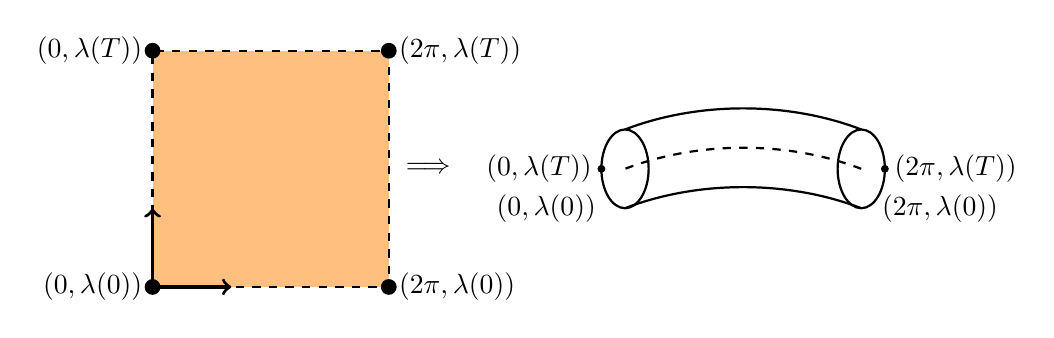
\begin{tikzpicture}
        \fill[orange,opacity=0.5] (0,0) rectangle (3,3);
        \draw[dashed,thick] (0,0) node[left]{$(0,\lambda(0))$} -- (3,0) node[right]{$(2\pi,\lambda(0))$} -- (3,3) node[right]{$(2\pi,\lambda(T))$} -- (0,3) node[left]{$(0,\lambda(T))$} -- cycle;
        \fill[black] (0,0) circle (0.1);
        \fill[black] (3,0) circle (0.1);
        \fill[black] (3,3) circle (0.1);
        \fill[black] (0,3) circle (0.1);
        \draw[->,very thick] (0,0) -- (1,0);
        \draw[->,very thick] (0,0) -- (0,1);
        \node at (3.5,1.5) {$\Longrightarrow$};
        \draw[thick] (9,1) arc (60:120:3 and 2);
        \draw[thick] (9,2) arc (60:120:3 and 2);
        \draw[dashed,thick] (9,1.5) arc (60:120:3 and 2);
        \draw[thick] (6,1.5) ellipse (0.3 and 0.5);
        \draw[thick] (9,1.5) ellipse (0.3 and 0.5);
        \fill[black] (5.7,1.5) node[left]{$(0,\lambda(T))$} circle (0.05);
        \node at (5,1) {$(0,\lambda(0))$};
        \fill[black] (9.3,1.5) node[right]{$(2\pi,\lambda(T))$} circle (0.05);
        \node at (10,1) {$(2\pi,\lambda(0))$};
    \end{tikzpicture}
\end{center}
由于时间和$q$空间的周期性,一个周期的态最多只能相差一个相因子,所以我们有
\begin{equation}
    \begin{split}
        |u_n(0,\lambda(t))\rangle&=e^{i\theta_\lambda^n(\lambda(t))}|u_n(2\pi,\lambda(t))\rangle\\
        |u_n(q_\alpha,\lambda(0))\rangle&=e^{i\theta_{q_\alpha}^n(q_\alpha)}|u_n(q_\alpha,\lambda(T))\rangle
    \end{split}
\end{equation}
带入Berry联络里计算得到
\begin{equation}
    \begin{split}
        A_\lambda^n(2\pi,\lambda(t))&=\langle u_n(2\pi,\lambda(t))|i\frac{\partial}{\partial\lambda}|u_n(2\pi,\lambda)\rangle\\
        &=\langle u_n(0,\lambda(t))|e^{-i\theta_\lambda^n(\lambda(t))}i\frac{\partial}{\partial\lambda}e^{-i\theta_\lambda^n(\lambda(t))}|u_n(0,\lambda(t))\rangle\\
        &=A_\lambda^n(0,\lambda(t))+\frac{\partial\theta_\lambda^n(\lambda(t))}{\partial \lambda}
    \end{split}
\end{equation}
\begin{equation}
    A_{q_\alpha}^n(q_\alpha,\lambda(T))=A_{q_\alpha}^n(q_\alpha,\lambda(0))+\frac{\partial\theta_{q_\alpha}^n(q_\alpha)}{\partial q_\alpha}
\end{equation}
带入极化强度表达式得到
\begin{equation}
    \begin{split}
        \Delta P_\alpha&=-\frac{e}{2\pi}\sum_{n}\int_{\lambda(0)}^{\lambda(T)}\mathrm{d}\lambda\frac{\partial\theta_\lambda^n(\lambda(t))}{\partial\lambda}+\frac{e}{2\pi}\sum_{n}\int_{BZ}\mathrm{d}q_\alpha\frac{\partial \theta_{q_\alpha}^n(q_\alpha)}{\partial q_\alpha}\\
        &=-\frac{e}{2\pi}\sum_{n}[\theta_\lambda^n(\lambda(T))-\theta_\lambda^n(\lambda(0))-\theta_{q_\alpha}^n(2\pi)+\theta_{q_\alpha}^n(0)]
    \end{split}
\end{equation}
由于周期性,上式相因子叠加后只能为$2\pi\nu,\nu\in\mathbf{Z}$. 所以最后结果为
\begin{equation}
    \Delta P_\alpha=-e\nu a
\end{equation}
其中$a$是补上的晶格常数。这里出现的$\nu$作为绝热输运的拓扑不变量。

布洛赫基到瓦尼尔基变换
\begin{equation}
    |R,n\rangle=\frac{1}{(2\pi)^d}\int \mathrm{d}ke^{-i\mathbf{k}\cdot(\mathbf{R}-\mathbf{r})}|u_n{k}\rangle
\end{equation}
King-Smith证明了极化强度可以定义为$\mathbf{R}=0$时对所有Wannier态的电荷中心的能带求和
\begin{equation}
    \mathbf{P}=-e\sum_{n}\langle\mathbf{R}=0,n|r|\mathbf{R}=0,n\rangle=-\frac{e}{2\pi}\oint\mathrm{d}\mathbf{k}\cdot \mathbf{A}(\mathbf{k})
\end{equation}
其中$A(\mathbf{k})=i\sum_{n}\langle u_n(k)|\nabla_{\mathbf{k}}|u_n(\mathbf{k})\rangle$. 最后一个等号利用了$\mathbf{r}=i\nabla_{\mathbf{k}}$
\subsection{Thouless电荷泵}
在一维绝缘体的循环绝热演化中
\begin{equation}
    H(k,t+T)=H(k,t)
\end{equation}
通过绝缘体泵浦的电荷总是整数,它被定义为一个拓扑不变量,也就是电极化矢量
\begin{equation}
    \Delta P=-\frac{e}{2Pi}[A(k,T)-A(k,0)]\mathrm{d}k=-nea
\end{equation}
我们举个例子来说明电荷泵浦过程,Rice-Mele模型:
\begin{equation}
    H=h_{st}(t)\sum_{i}(-1)^ic_i^\dagger c_i+\frac{1}{2}\sum_{i=1}^N[t_0+\delta(t)(-1)^i]c_i^\dagger c_{i+1}+h.c.
\end{equation}
其中
\begin{equation}
    (\delta(t),h_{st}(t))=\left(\delta_0\cos\frac{2\pi t}{T},h_0\sin\frac{2\pi t}{T}\right)
\end{equation}
这里$N$是偶数,这是一个时间依赖的模型:$\delta(t)$表示在交错子格或者二聚体中第$i$个和$i+1$个电子从平衡位置的偏移。$\delta(t)$和$h_{st}(t)$都是时间$t$以$T$为周期的函数。

哈密顿可以约化成两个子格系统
\begin{equation}
    H=h_{st}(t)\sum_{j=1}^Na_j^\dagger a_j-h_{st}(t)\sum_{j=1}b_j^\dagger b_j+\frac{1}{2}\sum_{j=1}^{N}(t_0-\delta(t))a_j^\dagger b_j+\frac{1}{2}\sum_{j=1}^{N}[t_0+\delta(t)]a_{j+1}^\dagger b_{j}+h.c.
\end{equation}
\begin{center}
    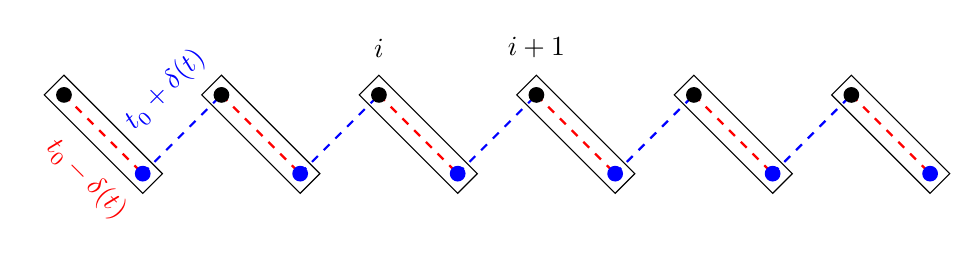
\begin{tikzpicture}
        \draw (-0.25,0) -- (1,-1.25) -- (1.25,-1) -- (0,0.25) -- cycle;
        \draw (1.75,0) -- (3,-1.25) -- (3.25,-1) -- (2,0.25) -- cycle;
        \draw (3.75,0) -- (5,-1.25) -- (5.25,-1) -- (4,0.25) -- cycle;
        \draw (5.75,0) -- (7,-1.25) -- (7.25,-1) -- (6,0.25) -- cycle;
        \draw (7.75,0) -- (9,-1.25) -- (9.25,-1) -- (8,0.25) -- cycle;
        \draw (9.75,0) -- (11,-1.25) -- (11.25,-1) -- (10,0.25) -- cycle;
        \draw[dashed,thick,red] (0,0) --node[below=1em,rotate=-45]{$t_0-\delta(t)$} (1,-1);
        \draw[dashed,thick,red] (2,0) -- (3,-1);
        \draw[dashed,thick,red] (4,0) -- (5,-1);
        \draw[dashed,thick,red] (6,0) -- (7,-1);
        \draw[dashed,thick,red] (8,0) -- (9,-1);
        \draw[dashed,thick,red] (10,0) -- (11,-1);
        \draw[dashed,thick,blue] (1,-1) --node[above=1em,rotate=45]{$t_0+\delta(t)$} (2,0);
        \draw[dashed,thick,blue] (3,-1) -- (4,0);
        \draw[dashed,thick,blue] (5,-1) -- (6,0);
        \draw[dashed,thick,blue] (7,-1) -- (8,0);
        \draw[dashed,thick,blue] (9,-1) -- (10,0);
        \fill (0,0) circle (0.1);
        \fill (2,0) circle (0.1);
        \fill (4,0)node[above=1em]{$i$} circle (0.1);
        \fill (6,0)node[above=1em]{$i+1$} circle (0.1);
        \fill (8,0) circle (0.1);
        \fill (10,0) circle (0.1);
        \fill[blue] (1,-1) circle (0.1);
        \fill[blue] (3,-1) circle (0.1);
        \fill[blue] (5,-1) circle (0.1);
        \fill[blue] (7,-1) circle (0.1);
        \fill[blue] (9,-1) circle (0.1);
        \fill[blue] (11,-1) circle (0.1);
    \end{tikzpicture}
\end{center}
我们考虑一个偶数个格子的系统,采用周期边界条件。做傅里叶变换
\begin{equation}
    \begin{split}
        a_k=\frac{1}{\sqrt{Na}}\sum_{j=1}^{N}a_j e^{-ikja}\\
        b_k=\frac{1}{\sqrt{Na}}\sum_{j=1}^{N}b_je^{-ik(j+\frac{1}{2})a}
    \end{split}
\end{equation}
得到
\begin{equation}
    H(t)=h_{st}\sum_{k\in BZ}(a_k^\dagger a_k-b_k^\dagger b_k)+\frac{1}{2}(t_0-\delta(t))\sum_{k}a_k^\dagger b_k e^{i\frac{ka}{2}}+\frac{1}{2}(t_0+\delta(t))\sum_{k}a_k^\dagger b_k e^{-i\frac{ka}{2}}+h.c.
\end{equation}
\begin{equation}
    H(t)=\sum_{k\in BZ}\begin{pmatrix}
        a_k^\dagger&b_k^\dagger
    \end{pmatrix}H(k,t)\begin{pmatrix}
        a_k\\
        b_k
    \end{pmatrix},\quad H(k,t)=\begin{pmatrix}
        h_{st}(t)&t_0\cos\frac{ka}{2}-i\delta(t)\sin\frac{ka}{2}\\
        t_0\cos\frac{ka}{2}+i\delta(t)\sin\frac{ka}{2}&-h_{st}(t)
    \end{pmatrix}
\end{equation}
\begin{equation}
    H(k,t)=d(k,t)\cdot\sigma
\end{equation}
其中
\begin{equation}
    \begin{split}
        &d_x(k,t)=t_0\cos\frac{ka}{2},\quad d_y(k,t)=\delta(t)\sin\frac{ka}{2},\quad d_z(k,t)=h_{st}(t)
    \end{split}
\end{equation}
$t$时刻两带色散关系为
\begin{equation}
    E(k,t)=\pm|d(k,t)|=\pm\sqrt{t_0^2\cos^2\frac{ka}{2}+\delta_0^2\cos\frac{2\pi t}{T}\sin^2\frac{ka}{2}+h_0^2\sin^2\frac{2\pi t}{T}}
\end{equation}
\begin{center}
    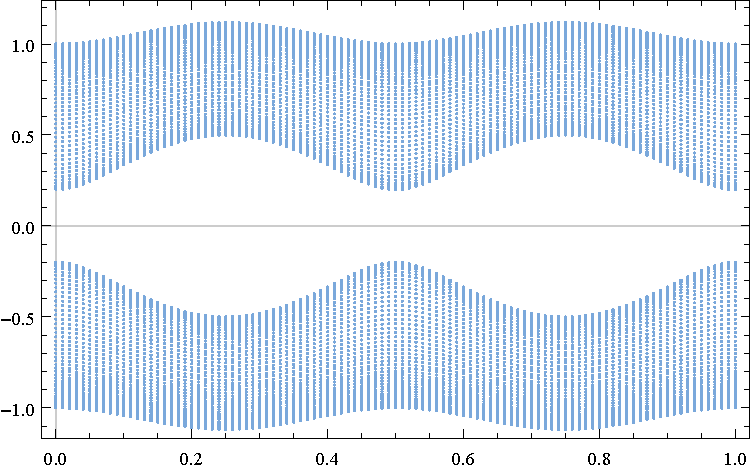
\includegraphics[height=2in]{rice-mele.pdf}
\end{center}
当$h_0=0$或$\delta_0=0$并且$t_0=0$时,出现简并点。两带之间的能隙为$\Delta E=\min(2|t_0|,2|h_0|,2|\delta_0|)$. 所以绝热条件要求有$T\gg\frac{\hbar}{\min(2|t_0|,2|h_0|,2|\delta_0|)}$. 如果低能带全部占满,在循环绝热演化中的电荷泵浦与基态的Chern数有关$\Delta P=-ea\mathcal{C}$
\begin{equation}
    \begin{split}
        \mathcal{C}&=\frac{1}{2\pi}\int_{0}^{T}\mathrm{d}t\int_{BZ}\mathrm{d}k\Omega_{k,t}^n\\
        &=\frac{1}{4\pi}\int_{BZ}\mathrm{d}k\int_{0}^{T}\mathrm{d}t\hat{d}(k,t)\cdot(\partial_k\hat{d}(k,t)\times\partial_t\hat{d}(k,t))\\
        &=\mathrm{sgn}(t_0h_0\delta_0)
    \end{split}
\end{equation}
因为$t$的周期性,$k-t$平面形成一个闭合的环面。我们可以看到只要$t_0,g_0\delta_0\neq0$,Chern数总是为$1$或者$-1$. 拓扑量子相变发生在$h_0=0,t_0=0$或者$\delta_0=0,t_0=0$, 其中无论其中任何一个参数改变符号,Chern数都会改变符号。

电荷泵浦可以通过开放链的末端态来理解。当$h_{st}=0,\delta(t)\neq0$时,Rice-Mele模型化简为SSH模型。$t=0$时,$(\delta(t),h_{st}(t))=(+\delta_0,0)$,从$i=1$开始,沿着格点的隧穿振幅为$t_0-\delta_0,t_0+\delta_0,t_0-\delta_0,\cdots$. 假设$t_0>\delta_0>0$. 在这种情况下,在链的两端分别存在两个零能的末端态,这两个末端在$h_0=0$简并。半满情况下,一个电子平均占据两个格点,我们假设右边的末端态被电子占据,左边的末端态空占据。随着时间的增加,On-site项$h_st(t)$把末端态从零能拉到价带,一个被拉到正能带,一个被拉到负能带。在$t=\frac{T}{2}$时,$(\delta(t),h_{st}(t))=(-\delta_0,0)$. 隧穿振幅变成$t_0+\delta_0,t_0-\delta_0,t_0+\delta_0,\cdots$. 在这种情况下,由于两个末端态演化到了体态,所以此时末端态消失。当$t$连续增加,末端态重新出现。但是占据电子的末端态变成了左边,右边的末端态则成了空占据。在$t=T$时,$(\delta(t),h_{st}(t))=(+\delta_0,0)$. 隧穿振幅变回$t=0$的状态。哈密顿重新回到了$t=0$的样子。虽然能量本征态没有发生改变,由于半满时基态的双重简并,电子的构型发生了改变:$t=0$时处于右边末端态的电子,在$t=T$时被输运倒了左边的末端态。通过这种方式,电子从左边被泵浦到了右边。瞬时谱如下:
\begin{center}
    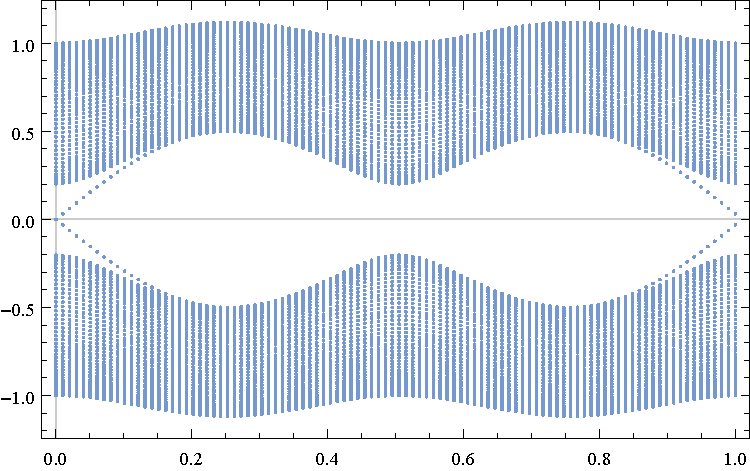
\includegraphics[height=2in]{rice-mele1.pdf}
\end{center}
\subsection{Fu-Kane泵浦}
Fu和Kane通过推广无自旋的Rice-Mele模型提出了自旋$\frac{1}{2}$的自旋泵浦电子模型:
\begin{equation}
    H=h_{st}(t))\sum_{i,\sigma=\pm 1}(-1)^ic_{i,\sigma}^\dagger\sigma_{\sigma\sigma'}^zc_{i,\sigma'}+\frac{1}{2}\sum_{i,\sigma=\pm1}[t_0+(-1)^i\delta(t)]c_{i,\sigma}^\dagger c_{i+1,\sigma}+h.c.
\end{equation}
其中$(\delta(t),h_{st}(t))=(\delta_0\cos\frac{2\pi t}{T},h_0\sin\frac{2\pi t}{T})$, 哈密顿可以写成三项
\begin{equation}
    \begin{split}
        H_0&=\frac{1}{2}\sum_{i,\sigma=\pm1}t_0c_{i,\sigma}^\dagger c_{i+1,\sigma}+h.c.\\
        V_h&=h_{st}(t)\sum_{i,\sigma=\pm 1}(-1)^ic_{i,\sigma}^\dagger\sigma_{\sigma\sigma'}c_{i,\sigma'}\\
        V_t&=\frac{1}{2}\sum_{i,\sigma=\pm 1}\sum_{i,\sigma}(-1)^i\delta(t)c_{i,\sigma}^\dagger c_{i+1,\sigma}+h.c.
    \end{split}
\end{equation}

引入交错磁场替代On-site. 我们选择$\sigma_z$本征态作为基底,令$\phi_{k,\uparrow}^\dagger=(a_{k,\uparrow}^\dagger,b_{k,\uparrow}^\dagger),\phi_{k,\downarrow}^\dagger=(a_{k,\downarrow}^\dagger,b_{k,\downarrow}^\dagger)$. 这个模型是一个根据自旋向上和自旋向下的分块对角矩阵
\begin{equation}
    H=\sum_{k}\begin{pmatrix}
        \phi_{k,\uparrow}^\dagger&\phi_{k,\downarrow}^\dagger
    \end{pmatrix}\begin{pmatrix}
        d_+\cdot\sigma&0\\
        0&d_{-}\cdot\sigma
    \end{pmatrix}\begin{pmatrix}
        \phi_{k,\uparrow}\\
        \phi_{k,\downarrow}
    \end{pmatrix}
\end{equation}
其中
\begin{equation}
    \begin{array}{l}
        \left(\mathbf{d}_{\pm}\right)_{x}=t_0\cos\frac{ka}{2} \\
        \left(\mathbf{d}_{\pm}\right)_{y}=\delta(t) \sin \frac{ka}{2}\\
        \left(\mathbf{d}_{\pm}\right)_{z}=\pm h_{s t}(t)
        \end{array}
\end{equation}
这样,电子自旋向上和自旋向下是解耦的。在$(\mathbf{d}_{\pm})_z$里差一个负号。这样对于自旋向上和自旋向下的Berry曲率也差一个负号。当$t$从$0$增加到$T$时,如果自旋向上的电子从左边移动到右边,则必定有另一个自旋向下的电子从右边移动到左边:
\begin{equation}
    \Delta P_{\uparrow}=+ea
\end{equation}
\begin{equation}
    \Delta P_{\downarrow}=-ea
\end{equation}
总的来说,循环演化中没有电荷泵浦。除了由电子自旋向上和自旋向下同时反方向移动导致的电子在末端交换自旋。当$s_z$是守恒量时,这个想法可以用来描述量子化自旋泵浦。

在下图中,我们描述了绝热循环代表性点处强耦合极限的基态。在$t=\frac{T}{4}$和$T=\frac{3T}{4}$处,$h_{st}(t)$占主导地位,系统形成Neel态。在$t=0$和$t=\frac{T}{2}$时,$V_t$占主导地位,单态电子对交错占据化学键形成二聚体。值得注意,$t=\frac{T}{2}$与$t=0$的基态可以通过末端未配对电子来区分。
\begin{center}
    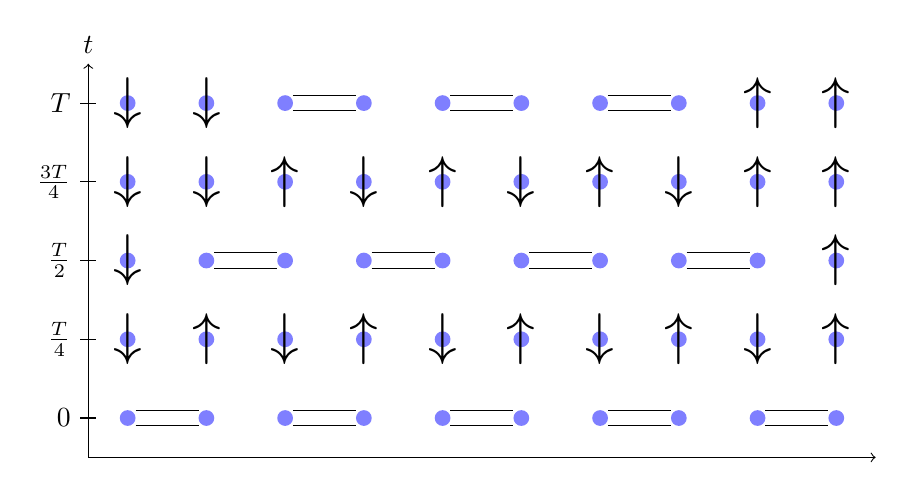
\begin{tikzpicture}
        \draw[->] (0,0) -- (10,0);
        \draw[->] (0,0) -- (0,5)node[above]{$t$};
        \draw (-0.1,0.5)node[left]{$0$} -- (0.1,0.5);
        \draw (-0.1,1.5)node[left]{$\frac{T}{4}$} -- (0.1,1.5);
        \draw (-0.1,2.5)node[left]{$\frac{T}{2}$} -- (0.1,2.5);
        \draw (-0.1,3.5)node[left]{$\frac{3T}{4}$} -- (0.1,3.5);
        \draw (-0.1,4.5)node[left]{$T$} -- (0.1,4.5);
        \fill[blue,opacity=0.5] (0.5,0.5) circle (0.1);
        \fill[blue,opacity=0.5] (1.5,0.5) circle (0.1);
        \fill[blue,opacity=0.5] (2.5,0.5) circle (0.1);
        \fill[blue,opacity=0.5] (3.5,0.5) circle (0.1);
        \fill[blue,opacity=0.5] (4.5,0.5) circle (0.1);
        \fill[blue,opacity=0.5] (5.5,0.5) circle (0.1);
        \fill[blue,opacity=0.5] (6.5,0.5) circle (0.1);
        \fill[blue,opacity=0.5] (7.5,0.5) circle (0.1);
        \fill[blue,opacity=0.5] (8.5,0.5) circle (0.1);
        \fill[blue,opacity=0.5] (9.5,0.5) circle (0.1);
        \fill[blue,opacity=0.5] (0.5,1.5) circle (0.1);
        \fill[blue,opacity=0.5] (1.5,1.5) circle (0.1);
        \fill[blue,opacity=0.5] (2.5,1.5) circle (0.1);
        \fill[blue,opacity=0.5] (3.5,1.5) circle (0.1);
        \fill[blue,opacity=0.5] (4.5,1.5) circle (0.1);
        \fill[blue,opacity=0.5] (5.5,1.5) circle (0.1);
        \fill[blue,opacity=0.5] (6.5,1.5) circle (0.1);
        \fill[blue,opacity=0.5] (7.5,1.5) circle (0.1);
        \fill[blue,opacity=0.5] (8.5,1.5) circle (0.1);
        \fill[blue,opacity=0.5] (9.5,1.5) circle (0.1);
        \fill[blue,opacity=0.5] (0.5,2.5) circle (0.1);
        \fill[blue,opacity=0.5] (1.5,2.5) circle (0.1);
        \fill[blue,opacity=0.5] (2.5,2.5) circle (0.1);
        \fill[blue,opacity=0.5] (3.5,2.5) circle (0.1);
        \fill[blue,opacity=0.5] (4.5,2.5) circle (0.1);
        \fill[blue,opacity=0.5] (5.5,2.5) circle (0.1);
        \fill[blue,opacity=0.5] (6.5,2.5) circle (0.1);
        \fill[blue,opacity=0.5] (7.5,2.5) circle (0.1);
        \fill[blue,opacity=0.5] (8.5,2.5) circle (0.1);
        \fill[blue,opacity=0.5] (9.5,2.5) circle (0.1);
        \fill[blue,opacity=0.5] (0.5,3.5) circle (0.1);
        \fill[blue,opacity=0.5] (1.5,3.5) circle (0.1);
        \fill[blue,opacity=0.5] (2.5,3.5) circle (0.1);
        \fill[blue,opacity=0.5] (3.5,3.5) circle (0.1);
        \fill[blue,opacity=0.5] (4.5,3.5) circle (0.1);
        \fill[blue,opacity=0.5] (5.5,3.5) circle (0.1);
        \fill[blue,opacity=0.5] (6.5,3.5) circle (0.1);
        \fill[blue,opacity=0.5] (7.5,3.5) circle (0.1);
        \fill[blue,opacity=0.5] (8.5,3.5) circle (0.1);
        \fill[blue,opacity=0.5] (9.5,3.5) circle (0.1);
        \fill[blue,opacity=0.5] (0.5,4.5) circle (0.1);
        \fill[blue,opacity=0.5] (1.5,4.5) circle (0.1);
        \fill[blue,opacity=0.5] (2.5,4.5) circle (0.1);
        \fill[blue,opacity=0.5] (3.5,4.5) circle (0.1);
        \fill[blue,opacity=0.5] (4.5,4.5) circle (0.1);
        \fill[blue,opacity=0.5] (5.5,4.5) circle (0.1);
        \fill[blue,opacity=0.5] (6.5,4.5) circle (0.1);
        \fill[blue,opacity=0.5] (7.5,4.5) circle (0.1);
        \fill[blue,opacity=0.5] (8.5,4.5) circle (0.1);
        \fill[blue,opacity=0.5] (9.5,4.5) circle (0.1);
        \draw (0.6,0.6) -- (1.4,0.6);
        \draw (0.6,0.4) -- (1.4,0.4);
        \draw (2.6,0.6) -- (3.4,0.6);
        \draw (2.6,0.4) -- (3.4,0.4);
        \draw (4.6,0.6) -- (5.4,0.6);
        \draw (4.6,0.4) -- (5.4,0.4);
        \draw (6.6,0.6) -- (7.4,0.6);
        \draw (6.6,0.4) -- (7.4,0.4);
        \draw (8.6,0.6) -- (9.4,0.6);
        \draw (8.6,0.4) -- (9.4,0.4);
        \node at (0.5,1.5) {\huge{$\downarrow$}};
        \node at (1.5,1.5) {\huge{$\uparrow$}};
        \node at (2.5,1.5) {\huge{$\downarrow$}};
        \node at (3.5,1.5) {\huge{$\uparrow$}};
        \node at (4.5,1.5) {\huge{$\downarrow$}};
        \node at (5.5,1.5) {\huge{$\uparrow$}};
        \node at (6.5,1.5) {\huge{$\downarrow$}};
        \node at (7.5,1.5) {\huge{$\uparrow$}};
        \node at (8.5,1.5) {\huge{$\downarrow$}};
        \node at (9.5,1.5) {\huge{$\uparrow$}};
        \node at (0.5,2.5) {\huge{$\downarrow$}};
        \draw (1.6,2.6) -- (2.4,2.6);
        \draw (1.6,2.4) -- (2.4,2.4);
        \draw (3.6,2.6) -- (4.4,2.6);
        \draw (3.6,2.4) -- (4.4,2.4);
        \draw (5.6,2.6) -- (6.4,2.6);
        \draw (5.6,2.4) -- (6.4,2.4);
        \draw (7.6,2.6) -- (8.4,2.6);
        \draw (7.6,2.4) -- (8.4,2.4);
        \node at (9.5,2.5) {\huge{$\uparrow$}};
        \node at (0.5,3.5) {\huge{$\downarrow$}};
        \node at (1.5,3.5) {\huge{$\downarrow$}};
        \node at (2.5,3.5) {\huge{$\uparrow$}};
        \node at (3.5,3.5) {\huge{$\downarrow$}};
        \node at (4.5,3.5) {\huge{$\uparrow$}};
        \node at (5.5,3.5) {\huge{$\downarrow$}};
        \node at (6.5,3.5) {\huge{$\uparrow$}};
        \node at (7.5,3.5) {\huge{$\downarrow$}};
        \node at (8.5,3.5) {\huge{$\uparrow$}};
        \node at (9.5,3.5) {\huge{$\uparrow$}};
        \node at (0.5,4.5) {\huge{$\downarrow$}};
        \node at (1.5,4.5) {\huge{$\downarrow$}};
        \draw (2.6,4.6) -- (3.4,4.6);
        \draw (2.6,4.4) -- (3.4,4.4);
        \draw (4.6,4.6) -- (5.4,4.6);
        \draw (4.6,4.4) -- (5.4,4.4);
        \draw (6.6,4.6) -- (7.4,4.6);
        \draw (6.6,4.4) -- (7.4,4.4);
        \node at (8.5,4.5) {\huge{$\uparrow$}};
        \node at (9.5,4.5) {\huge{$\uparrow$}};
    \end{tikzpicture}
\end{center}

电子自旋不服从基本守恒定律。自旋泵浦的概念不能简单的推广到$s_z$不守恒的情况。然而$Fu-Kane$提出了一个在自旋自由度不守恒时的类似的物理发生。考虑一个自旋轨道耦合(DMI)的额外项,
\begin{equation}
    V_{so}=\sum_{i,\sigma,\sigma'}i\mathbf{e}_{so}\cdot\sigma_{\sigma\sigma'}\left(c_{i,\sigma}^\dagger c_{i+1,\sigma'}-c_{i+1,\sigma}^\dagger c_{i,\sigma'}\right)
\end{equation}
其中$\mathbf{e}_{so}$是表征自旋轨道相互作用的一个任意矢量。通过这种方式,$z$分量的自旋$\sigma^z$不再是一个好量子数
\begin{equation}
    V_{so}=-2\sum_{k,\sigma,\sigma'}\mathbf{e}_{so}\cdot\sigma_{\sigma\sigma'}\sin\frac{ka}{2}(a_{k\sigma}^\dagger b_{k\sigma'}+b_{k\sigma}^\dagger a_{k\sigma'})
\end{equation}
自旋轨道耦合破坏了$s_z$的守恒,但系统仍然有额外的对称性,时间反演对称性。哈密顿在TR下满足
\begin{equation}
    H(-t)=\Theta H(t)\Theta^{-1}
\end{equation}
对于绝热循环演化,我们有
\begin{equation}
    H(t)=H(t+T)
\end{equation}
存在两个点$t_1=0,t_2=\frac{T}{2}$,在这两点处时间反演不变
\begin{equation}
    H(t_i)=\Theta H(t_i)\Theta^{-1},\quad i=1,2
\end{equation}
这两个点的存在在循环泵浦的拓扑分类里起到至关重要的作用。

一般来说,在远离守恒定律的情况下,系统将不会有能级交错,在循环的前后,系统将一直停留在相同的态上。在电荷泵浦的情况下,能级交错由电荷守恒所保护。$t_1$和$t_2$处的能级交错由时间反演对称所保护。在这两点处,存在着Kramers简并:两个态互相时间反演对称,并且有相同的能量。Fu和Kane提出引入时间反演极化的概念,在自旋泵中将其量子化。
\subsection{整数霍尔效应:Laughlin argument}
Laughlin指出,霍尔电导的量子化是规范不变性和迁移率隙存在的结果。考虑沿着$y$方向卷成圆柱的二维电子气体。磁通$\phi$穿过圆筒,随时间变化非常缓慢。假设系统有能隙,且费米能在能隙处。根据法拉第定律变化的磁场诱导绕着磁通$\phi$的电场$E_y$. 霍尔电流密度$J_x$为
\begin{equation}
    J_x=\sigma_{xy}E_y
\end{equation}
$\sigma_{xy}$是霍尔电导。电荷连续性条件得到流过圆柱体的电荷$Q$是
\begin{equation}
    \frac{\mathrm{d}Q}{\mathrm{d}t}=-\oint\mathrm{d}l\cdot J_x=-\sigma_{xy}\oint\mathrm{d}l\cdot E_y
\end{equation}
利用Stokes定理得到
\begin{equation}
    \oint \mathrm{d} l \cdot E_{y}=\int \mathrm{d} \mathbf{S} \cdot \nabla \times E_{y}
\end{equation}
更进一步,从法拉第定律$\nabla\times \mathbf{E}=-\frac{\partial B}{\partial t}$得到
\begin{equation}
    \frac{\mathrm{d}Q}{\mathrm{d}t}=\sigma_{xy}\iint\mathrm{d}S\cdot\frac{\partial\mathbf{B}}{\partial t}=\sigma_{xy}\frac{\mathrm{d}\phi}{\mathrm{d}t}
\end{equation}
或者
\begin{equation}
    \Delta Q=\sigma_{xy}\Delta \phi
\end{equation}
磁通变化为磁通量子$\Delta\phi=\phi_0=\frac{2\pi\hbar}{e}$,霍尔电导变成$\sigma_{xy}=\frac{e}{h}\Delta Q$. 这样霍尔电导是由改变单位磁通量子后电荷转移$\Delta Q$来决定的。

$\Delta Q$的值是多少?在目前的几何结构中,圆柱体中的磁通量将导致磁矢势的规范变换,
\begin{equation}
    p+eA\rightarrow p+e(A+\delta A)
\end{equation}
这里$\delta A=\frac{\hbar}{e}\nabla\lambda$. 波函数在规范变换后多了个相因子
\begin{equation}
    \psi(r)\rightarrow e^{i\lambda(r)}\psi(r)
\end{equation}
对于单位量子磁通$\oint \delta A\cdot\mathrm{d}l=\phi_0$, 有$\lambda(r,\phi=\phi_0)-\lambda(r,\phi=0)=2\pi$. 这样在改变一个单位磁通后的本征态不变
\begin{equation}
    H(\phi=\phi_0)=H(\phi=0)
\end{equation}
对于多体系统,一个量子通量变化后,电子的占据数可能会不同,
\begin{equation}
    \Delta Q=ne
\end{equation}
其中$n$是整数,并且有系统能带结构的拓扑所决定。因此,我们判断
\begin{equation}
    \sigma_{xy}=n\frac{e^2}{h}
\end{equation}
这个可以被看做电荷巨热泵浦在二维系统里的推广。

Fu-Kane泵浦是Laghlin argument的自旋版本,作为一个从整数霍尔效应到自旋霍尔效应的推广,就像从电荷泵浦到自旋泵浦一样。对于量子自旋系统,时间反演对称将会给一个不同的拓扑不变量。考虑相同形状的装置,一个磁通$\phi$穿过二维的圆柱,这将会导致物理态上一个额外的相位改变$e^{i2\pi\frac{\phi}{\phi_0}}$. 在能带理论中,磁通起着边缘晶格动量$k_x$的作用。随着时间$t$变化,磁通从$\phi=0$增加到$phi=\phi_0$构成一个绝热循环演化。在$\phi=0$和$\phi=\frac{\phi_0}{2}$处存在Kramers简并
\begin{equation}
    \begin{split}
        H(0)&=\Theta H(0)\Theta^{-1}\\
        H(\frac{\phi_0}{2})&=\Theta H(\frac{\phi_0}{2})\Theta^{-1}
    \end{split}
\end{equation}
因此,半通量量子的变化将改变两端的电子宇称数。
\subsection{时间反演算符}
在经典物理中,牛顿定律由于包含了时间的二阶导,所以存在一个时间反演对称。$t\rightarrow -t$
\begin{equation}
    F=m\frac{\mathrm{d}^2x}{\mathrm{d}t^2}
\end{equation}
对于作用力与时间无关的情况,$\Theta F=F$
\begin{equation}
    \Theta F=\Theta m\frac{\mathrm{d}^2x}{\mathrm{d}t^2}=m\left(-\frac{\mathrm{d}}{\mathrm{d}t}\right)\left(-\frac{\mathrm{d}}{\mathrm{d}t}\right)x\Rightarrow F=m\frac{\mathrm{d}^2x}{\mathrm{d}t^2}
\end{equation}
对于麦克斯韦方程
\begin{equation}
    \begin{split}
        \nabla\cdot E&=\frac{\rho}{\epsilon_0}\\
        \nabla\times E&=-\frac{\partial B}{\partial t}\\
        \nabla\cdot B&=0\\
        \nabla\times B&=\mu_0J+\mu_0\epsilon_0\frac{\partial E}{\partial t}
    \end{split}
\end{equation}
两边同时作用时间反演算符$\Theta$
\begin{equation}
    \begin{split}
        \nabla\cdot \Theta E&=\frac{\rho}{\epsilon_0}\\
        \nabla\times \Theta E&=\frac{\partial \Theta B}{\partial t}\\
        \nabla\cdot \Theta B&=0\\
        \nabla\times \Theta B&=\mu_0\Theta J-\mu_0\epsilon_0\frac{\partial \Theta E}{\partial t}
    \end{split}
\end{equation}
在宏观上,麦克斯韦方程应该具有时间反演对称性,所以在时间反演的要求下必须有
\begin{equation}
    \Theta J=-J,\quad\Theta E=E,\quad\Theta B=-B
\end{equation}
对于量子系统,我们考虑态的时间演化$|\psi\rangle$.
\begin{equation}
    |\psi(t)\rangle=U(t)|\psi(0)\rangle
\end{equation}
其中时间演化算符的无穷小生成元正比于哈密顿。现在在时间演化算符上加上时间反演算符
\begin{equation}
    \Theta|\psi(t)\rangle=\Theta U(t)|\psi(0)\rangle\Rightarrow |\psi(-t)\rangle=\Theta U(t)\Theta^{-1} \Theta|\psi(0)\rangle\Rightarrow |\psi(-t)\rangle=\Theta U(t)\Theta^{-1}|\psi(0)\rangle
\end{equation}
所以我们有
\begin{equation}
    \Theta U(t)\Theta^{-1}=U(-t),\quad\Theta U(t)=U(-t)\Theta
\end{equation}
考虑时间演化算符的无穷小展开
\begin{equation}
    \Theta(1-\frac{i}{\hbar}Ht)=(1+\frac{i}{\hbar}Ht)\Theta\Rightarrow -\Theta iH=iH\Theta
\end{equation}
若$\Theta$是幺正算符,这意味着$\Theta H=-H\Theta$. 对于幺正的情况有${\Theta,H}=0$. 这个结果会导致负能解。
\begin{equation}
    H\Theta |E\rangle=-\Theta H|E\rangle=-E\Theta|E\rangle,E>0
\end{equation}
所以$\Theta|E\rangle$也是哈密顿算符的本征矢量,对应的能量本征值是$-E$. 除此之外,系统具有时间反演对称要求$[\Theta,H]=0$. 这导致了
\begin{equation}
    \Theta H=0
\end{equation}
由于$\Theta$必须是可逆的,这就只能是$H=0$. 在量子力学里为了解决这个矛盾,引入了反幺正算符$\Theta i=-i\Theta$. 这使得$[\Theta,H]=0$,正好和对称性条件一致。值得注意,在量子场论里,我们不能用$t\rightarrow-t$作为时间反演的定义。时间的流逝并不是各向同性的——固有时沿不同的世界线以不同的速率流逝。而在量子力学里,这个问题非常简单,因为在量子力学里,时间只是一个参数。这允许我们通过定义反幺正算符来避免量子力学中的这个问题。当我们引入时间反演作为反幺正算子时,我们避免了负能量。在量子场论中情况不同,负能量状态被重新解释为反粒子。

我们定义反幺正算子满足:
\begin{equation}
    \begin{aligned}
        \langle\tilde{\beta} \mid \tilde{\alpha}\rangle &=\langle\beta \mid \alpha\rangle^{*} \\
        \hat{\Theta}\left(c_{1}|\alpha\rangle+c_{2}|\beta\rangle\right) &=c_{1}^{*}|\tilde{\alpha}\rangle+c_{2}^{*}|\tilde{\beta}\rangle
        \end{aligned}
\end{equation}
其中$|\tilde{\alpha}\rangle\equiv\hat{\Theta}|\alpha\rangle,|\tilde{\beta}\rangle \equiv \hat{\Theta}|\beta\rangle$是反幺正变换后的态。如果我们令$c_1=i,c_2=0$则有
\begin{equation}
    \hat{\Theta} i|\alpha\rangle=-i|\tilde{\alpha}\rangle=-i \hat{\Theta}|\alpha\rangle
\end{equation}
所以有$\Theta i=-i\Theta$. 根据上面的定义,可以得到下列结论
\begin{enumerate}
    \item $\Theta i=-i\Theta$
    \item 实数与$\Theta$对易
    \item $\Theta$满足乘法分配律$\Theta(c_1|\alpha\rangle+c_2|\beta\rangle)=\Theta(c_1|\alpha\rangle)+\Theta(c_2|\beta\rangle)=c_1^*|\tilde{\alpha}\rangle+c_2^*|\tilde{\beta}\rangle$
\end{enumerate}
我们可以证明,幺正算符和反幺正算符的乘积依旧是一个反幺正算符,而两个反幺正算符的乘积则是幺正算符。具体简单证明一下。设$\Theta$是反幺正算符,$U$是幺正算符
\begin{equation}
    \langle \tilde{\beta}|\tilde{\alpha}\rangle=(\langle\beta|(\Theta U)^\dagger)(\Theta U|\alpha\rangle)=\langle\beta|U^\dagger\Theta^\dagger\Theta U|\alpha\rangle=(\langle\beta|U^\dagger U|\alpha\rangle)^*=\langle\beta|\alpha\rangle^*
\end{equation}
\begin{equation}
\langle\tilde{\beta}|\tilde{\alpha}\rangle=(\langle\beta|(\Theta_1\Theta_2)^\dagger)(\Theta_1\Theta_2|\alpha\rangle)=(\langle\beta|\Theta_2^\dagger\Theta_2|\alpha\rangle)^*=((\langle\beta|\alpha\rangle)^*)^*=\langle\beta|\alpha\rangle
\end{equation}
说明$\Theta_1\Theta_2$是幺正算符,$\Theta U$是反幺正算符。任意一个反幺正算符都可以写成幺正算符$U$和复共轭算符(K)的乘积
\begin{equation}
    \Theta=UK
\end{equation}
\begin{theorem}[Wigner定理]
    每一个保持转移概率的可逆算子都是幺正或反幺正的
\end{theorem}
我们仅仅在右矢量上定义了复共轭算符$K$,而不是左矢:$|\tilde{\alpha}\rangle=K|\alpha\rangle$. 复共轭算符并不改变基右矢。因此如果我们展开$|\alpha\rangle=\sum_{a}|a\rangle\langle a|\alpha\rangle$
\begin{equation}
    \begin{split}
        |\tilde{\alpha}\rangle&=K|\alpha\rangle=K\sum_{a}\langle a|\alpha\rangle|a\rangle\\
        &=\sum_a\langle a|\alpha\rangle^* K|a\rangle\\
        &=\sum_a\langle a|\alpha\rangle^*|a\rangle
    \end{split}
\end{equation}
这说明复共轭算符的定义依赖于基的选择。我们可以找到不同基之间复共轭算符的关系,假设旧基和新基之间由幺正变换$U$
\begin{equation}
    |b\rangle=U|a\rangle
\end{equation}
给定$K$在$\{|a\rangle\}$上不变,令$\tilde{K}|b\rangle=|b\rangle$. 我们得到
\begin{equation}
    \tilde{K}|b\rangle=|b\rangle\Rightarrow\tilde{K}U|a\rangle=U|a\rangle=UK|a\rangle\Rightarrow \tilde{K}=UKU^\dagger
\end{equation}
我们定义时间反演算符为一个反幺正算符。根据之前无穷小展开可以得到
\begin{equation}
    -\Theta iH=iH\Theta\Rightarrow i\Theta H=iH\Theta\Rightarrow[\Theta,H]=0
\end{equation}
在时间反演变换下定义
\begin{equation}
    \begin{aligned}
        |\tilde{\alpha}\rangle &=\hat{\Theta}|\alpha\rangle \\
        |\tilde{\beta}\rangle &=\hat{\Theta}|\beta\rangle
        \end{aligned}
\end{equation}
设线性变换$A$,$|\gamma\rangle=A^\dagger|\beta\rangle$, 对偶形式为$\langle\gamma|=\langle\beta|A$. 所以我们有
\begin{equation}
    \langle\beta|\hat{A}| \alpha\rangle=\langle\gamma \mid \alpha\rangle
\end{equation}
由于
\begin{equation}
    \langle\gamma \mid \alpha\rangle=\langle\alpha \mid \gamma\rangle^{*}=\langle\tilde{\alpha} \mid \tilde{\gamma}\rangle
\end{equation}
随遇反幺正算符我们有
\begin{equation}
    \begin{aligned}
        \langle\beta|\hat{A}| \alpha\rangle &=\langle\tilde{\alpha} \mid \tilde{\gamma}\rangle \\
        &=\langle\tilde{\alpha}|\hat{\Theta}| \gamma\rangle \\
        &=\left\langle\tilde{\alpha}\left|\hat{\Theta} \hat{A}^{\dagger}\right| \beta\right\rangle \\
        &=\left\langle\tilde{\alpha}\left|\hat{\Theta} \hat{A}^{\dagger} \hat{\Theta}^{-1} \hat{\Theta}\right| \beta\right\rangle \\
        &=\left\langle\tilde{\alpha}\left|\hat{\Theta} \hat{A}^{\dagger} \hat{\Theta}^{-1}\right| \tilde{\beta}\right\rangle
        \end{aligned}
\end{equation}
这说明反幺正算符作用在算符$A^\dagger$相似变换的作用。如果$A$是厄米算符.
\begin{equation}
    \langle\beta|A|\alpha\rangle=\langle\tilde{\alpha}|\Theta A\Theta^{-1}|\tilde{\beta}\rangle
\end{equation}
我们定义在时间反演下的奇偶性
\begin{equation}
    \Theta A\Theta^{-1}=\begin{cases}
        A&\text{偶}\\
        -A&\text{奇}
    \end{cases}
\end{equation}
我们计算期望
\begin{equation}
    \langle\alpha|A|\alpha\rangle=\pm\langle\tilde{\alpha}|A|\tilde{\alpha}\rangle
\end{equation}
在经典力学里,动量在时间反演的关系为$p\rightarrow-p$. 在量子力学里则表示成
\begin{equation}
    \langle\alpha|P|\alpha\rangle=-\langle\tilde{\alpha}|P|\tilde{\alpha}\rangle
\end{equation}
所以有$\Theta P\Theta^{-1}=-P$. 同样的与经典对应的坐标有$\Theta x\Theta^{-1}=x,\Theta J\Theta^{-1}=-J$

对于自旋$\frac{1}{2}$系统,时间反演会翻转自旋:$\Theta\sigma_\alpha\Theta^{-1}=-\sigma_\alpha$
其中$\alpha=x,y,z$. 注意到
\begin{equation}
    \begin{split}
        \sigma_y\sigma_x\sigma_y&=-\sigma_x\\
        \sigma_y\sigma_y\sigma_y&=\sigma_y\\
        \sigma_y\sigma_z\sigma_y&=-\sigma_z
    \end{split}
\end{equation}
由于$\sigma_y$是纯虚矩阵,$K\sigma_y=-\sigma_yK$. 所以我们构造时间反演算符为
\begin{equation}
    \Theta=i\sigma_yK
\end{equation}
显然,由于$K^2=1$. $\Theta^{-1}=-i\sigma_yK$. 
\begin{equation}
    \Theta^2=-1
\end{equation}
从转动的角度很容易推广到更高阶自旋情况,考虑$S\cdot n$的本征态$|n,+\rangle$,本征值为$+\frac{\hbar}{2}$.
\begin{equation}
    \begin{aligned}
        |n,+\rangle &=e^{-i S_{z} \alpha / \hbar} e^{-i S_{y} \beta / \hbar}|+\rangle \\
        \Theta|n,+\rangle &=\Theta e^{-i S_{z} \alpha / \hbar} e^{-i S_{y} \beta / \hbar} \Theta^{-1} \Theta|+\rangle
        \end{aligned}
\end{equation}
由于$\Theta S_\alpha\Theta^{-1}=-S_\alpha,\Theta i\Theta^{-1}=-i$
\begin{equation}
    \Theta|n,+\rangle=e^{-i S_{z} \alpha / \hbar} e^{-i S_{y} \beta / \hbar} \Theta|+\rangle=e^{-i S_{z} \alpha / \hbar} e^{-i S_{y} \beta / \hbar}|-\rangle=|n,-\rangle
\end{equation}
其中$\Theta|+\rangle=|-\rangle$,$|\pm\rangle$是$\sigma_z$的本征态。另一方面
\begin{equation}
    |n,-\rangle=e^{-i S_{z} \alpha / \hbar} e^{-i S_{y}(\pi+\beta) / \hbar}|+\rangle=e^{-i S_{z} \alpha / \hbar} e^{-i S_{y} \beta / \hbar} e^{-i S_{y} \pi / \hbar}|+\rangle
\end{equation}
注意到$K|+\rangle=|+\rangle$. 我们得到
\begin{equation}
    \Theta=e^{-i\pi S_y/\hbar}K=i\sigma_yK
\end{equation}
推广到更高阶自旋系统,对于角动量本征值为$j$的角动量算符,时间反演算符为
\begin{equation}
    \Theta=ie^{-i\pi J_y}K
\end{equation}
其中$J_y$是角动量$y$方向的分量。接下来我们证明一下$\Theta^2=(-1)^{2j}$. 我们考虑Schwinger变换,将系统看成$2j$个自旋$\frac{1}{2}$的电子直积
\begin{equation}
    S=\frac{N}{2},\quad\mathbf{S}=\sum_{i=1}^{N}\mathbf{S}_i,\quad|\frac{N}{2},\frac{N}{2}\rangle=\bigotimes_{i=1}^{N}|\frac{1}{2},\frac{1}{2}\rangle
\end{equation}
根据角动量升降算符可以有
\begin{equation}
    \begin{split}
        |\frac{N}{2},m\rangle&=\sqrt{\frac{(\frac{N}{2}+m)!}{N!(\frac{N}{2}-m)!}}(\frac{S_-}{\hbar})^{\frac{N}{2}-m}|\frac{N}{2},\frac{N}{2}\rangle\\
        &=\sqrt{\frac{(\frac{N}{2}+m)!}{N!(\frac{N}{2}-m)!}}(\frac{S_-}{\hbar})^{\frac{N}{2}-m}\bigotimes_{i=1}^{N}|\frac{1}{2},\frac{1}{2}\rangle
    \end{split}
\end{equation}
所以时间演化算符可以写成直积形式$\Theta=\bigotimes_{i=1}^{N}\sigma_y^iK$
\begin{equation}
    \Theta|\frac{N}{2},m\rangle=\bigotimes_{i=1}^{N}i\sigma_y^i|\frac{N}{2},m\rangle
\end{equation}
所以我们得到
\begin{equation}
    \begin{split}
        \Theta|\psi\rangle&=\Theta\sum_{m}\int\mathrm{d}r|r;\frac{N}{2},m\rangle\langle r;\frac{N}{2},m|\psi\rangle\\
        &=\sum_{m}\int\mathrm{d}r\langle \psi|r;\frac{N}{2},m\rangle\Theta(|r\rangle\otimes|\frac{N}{2},m\rangle)\\
        &=\sum_{m}\int\mathrm{d}r\langle\psi|r;\frac{N}{2},m\rangle|r\rangle\otimes\Theta|\frac{N}{2},m\rangle\\
        &=\sum_{m}\int\mathrm{d}r\langle\psi|r;\frac{N}{2},m\rangle|r\rangle\bigotimes_{i=1}^{N}i\sigma_y^i|\frac{N}{2},m\rangle
    \end{split}
\end{equation}
所以我们有$\Theta^2=(-1)^N=(-1)^{2j}$. 得证。

这意味着对于系统总角动量为奇数或者奇数个自旋$\frac{1}{2}$的费米子而言,存在Kramers简并。对于偶数个费米子系统或者总角动量为偶数的系统而言,则没有Kramers简并。
\begin{theorem}[Kramers简并]
    时间反演不变系统中奇数电子的能态至少有双重简并。
\end{theorem}
这里简单证明一下,对于$\Theta^2=-1$的系统,考虑两个态$|\psi\rangle,|\phi\rangle$
\begin{equation}
    \langle\psi|\Theta|\phi\rangle=\langle|\Theta\phi\rangle=\langle\Theta^2\phi|\Theta\psi\rangle=-\langle\phi|\Theta|\psi\rangle
\end{equation}
令$\psi=\phi$得到
\begin{equation}
    \langle\phi|\Theta|\phi\rangle=-\langle\phi|\Theta|\phi\rangle\Rightarrow\langle\phi|\Theta|\phi\rangle=0
\end{equation}
这意味着$|\phi\rangle$与$\Theta|\phi\rangle$正交。如果系统具有时间反演不变性,则有$[\Theta,H]=0$
\begin{equation}
    H|\phi\rangle=E|\phi\rangle\Rightarrow H\Theta|phi\rangle=\Theta H|\phi\rangle=E\Theta|\phi\rangle
\end{equation}
这说明$\Theta|\phi\rangle$也是$H$能量值为$E$的本征态。并且与$|\phi\rangle$正交。这种简并叫做Kramers简并
\subsection{时间反演对称和$Z_2$指标}
时间反演对称意味着$[H(r),\Theta]=0$, 其中时间反演算符为$\Theta=-i\sigma_y K$,$K$是复共轭算符。注意在能带里时间反演对称意味着
\begin{equation}
    H(-k)=\Theta H(k)\Theta^{-1}
\end{equation}
因为$k$是个好量子数,在哈密顿里已经替换了$p=-i\hbar\nabla$,动量在时间反演下会改变符号。在二维方格子的布里渊区内,有$4$个时间反演不变点。这些点满足$-\Gamma_i=\Gamma_i+n_i\mathbf{G}$. $\mathbf{G}$是倒格矢,$n_1=0,1$. 在这些点处,$\Gamma_i=\frac{n_i\mathbf{G}}{2}$:
\begin{equation}
    H(\Gamma_i)=\Theta H(\Gamma_i)\Theta^{-1}
\end{equation}
总是成立,因此在这些点处总是存在Kramers简并。一对这样的简并对$E_{2n-1}()k,E_{2n}(k)$叫做Kramers对。
\begin{figure}[h]
    \centering
    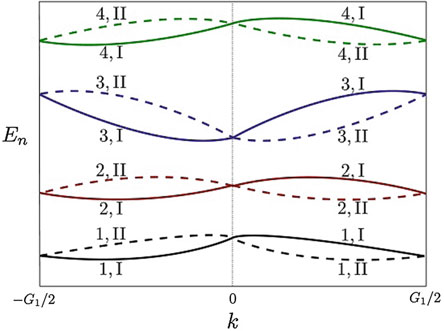
\includegraphics[width=3in]{Kramers.png}
    \caption{沿着一个方向倒格矢的能带结构图$E(k)$. Kramers对在TRI点处交叠。}\label{Kramers pairs}
\end{figure}
Kramers对分别被标记为$(n,I),(n,II)$. 一对Kramers对通过时间反演算符联系起来,同时有一个冗余相因子。它们在时间反演点发生交叠。如果Kramers对与其他对之间有一个有限能隙的间隔,可以定义一个拓扑不变量。

为了简单起见,我们考虑一个一维系统并且假设没有额外的简并除了时间反演对称性。因此$2N$个本征态可以分成$N$对能级,满足
\begin{equation}
    |u_n^I(-k)\rangle=-e^{i\chi_{k,n}}\Theta|u_n^{II}(k)\rangle
\end{equation}
两边乘以$\Theta$利用$\Theta^2=-1$(电子系统spin$\frac{1}{2}$)
\begin{equation}
    \Theta|u_n^I(-k)\rangle=-\Theta e^{i\chi_{k,n}}\Theta|u_n^{II}(k)\rangle=-\Theta e^{i\chi_{k,n}}\Theta^{-1}\Theta^2|u_n^{II}(k)\rangle=e^{-i\chi_{-k,n}}|u_n^{II}(k)\rangle
\end{equation}
替换$k\rightarrow -k$得到
\begin{equation}
    |u_n^{II}(-k)\rangle=e^{i\chi_{k,n}}\Theta|u_n^{II}(k)\rangle
\end{equation}
考虑自然单位,电荷单位$-e=1$. 与$s = I$或$II$任何一类相关的部分极化可以写成
\begin{equation}
    P^s=\int_{BZ}\frac{\mathrm{d}k}{2\pi}A^s(k)
\end{equation}
其中$A^s(k)=i\sum_{n}\langle u_n^s(k)|\nabla_k|u_n^s(k)\rangle$. 这个部分极化在$|u_n^I(k)\rangle$和$|u_n^{II}(k)\rangle$的相因子改变下是不变的。然而他们依赖于每个能带指标$I,II$的选择。为了明显的看出这种不变性,我们把积分拆成两部分
\begin{equation}
    P^I=\int_{0}^{\pi}\mathrm{d}k[A^I(k)+A^{I}(-k)]
\end{equation}
我们利用时间反演关系$\langle\Theta u_n^{II}{k}|\nabla_k|\Theta u_{n}(k)^{II}\rangle=-\langle u_n^{II}(k)|\nabla_k|u_n^{II}(k)\rangle$得到
\begin{equation}
    \begin{split}
        A^I(-k)&=i\sum_{n}\langle u_n^I(-k)|\nabla_{-k}|u_n^I(-k)\rangle\\
        &=-i\sum_{n}\langle \Theta u_n^{II}(k)|e^{-i\chi_{k,n}}\nabla_k e^{i\chi_{k,n}}|\Theta u_{n}^{II}(k)\rangle\\
        &=-i\sum_{n}\langle\Theta u_{n}^{II}(k)|i|\Theta u_{n}^{II}(k)\rangle\nabla_k\chi_{k,n}-i\sum_{n}\langle\Theta u_{n}^{II}(k)|\nabla_k|\Theta u_n^{II}(k)\rangle\\
        &=\nabla_k\chi_{k,n}+A^{II}(k)
    \end{split}
\end{equation}
值得注意,最后一个等号利用了时间反演算符的性质:
\begin{equation}
    \langle \beta|A|\alpha\rangle=\langle\Theta\alpha|\Theta A^\dagger\Theta^{-1}|\Theta\beta\rangle
\end{equation}
利用这个性质,我们可以得到
\begin{equation}
    \langle\Theta u_n^{II}(k)|\nabla_k|\Theta u_n^{II}(k)\rangle=\langle u_n^{II}(k)|\Theta\nabla_k\Theta^{-1}|u_n^{II}(k)\rangle=-\langle u_n^{II}(k)|\nabla_k|u_n^{II}(k)\rangle
\end{equation}
所以得到
\begin{equation}
    P^I=\int_0^\pi\frac{\mathrm{d}k}{2\pi}A(k)+\frac{1}{2\pi}\sum_n(\chi_{\pi,n}-\chi_{0,n})
\end{equation}
其中$A(k)=A^I(k)+A^{II}(k)$,我们引入一个$U(2N)$矩阵$w_{mn}=\langle u_m(-k)|\Theta|u_n(k)\rangle$,非零项只有次对角线上的项
\begin{equation}
    \begin{split}
        \langle u_n^I(-k)|\Theta|u_n^{II}(k)\rangle=-e^{-i\chi_{k,n}}\\
        \langle u_n^{II}(-k)|\Theta|u_n^I(k)\rangle=e^{-i\chi_{-k,n}}
    \end{split}
\end{equation}
$w$矩阵是所有n对应$2\times 2$矩阵$\begin{pmatrix}
    0&-e^{-i\chi_{k,n}}\\
    e^{-i\chi_{-k,n}}&0
\end{pmatrix}$的直和。在$k=0,\pi$处$w$是反对称矩阵。一个反对称矩阵可以用$Pfaffian$来表征,它的平方等于它的行列式。这样我们有
\begin{equation}
    Pf[w(\pi)]=\prod_{n}[-e^{-i\chi_{\pi,n}}],\quad Pf[w(0)]=\prod_{n}[-e^{-i\chi_{0,n}}],\quad\frac{Pf[w(\pi)]}{Pf[w(0)]}=e^{-i\sum_{n}(\chi_{\pi,n}-\chi_{0,n})}
\end{equation}
所以有
\begin{equation}
    i\ln\frac{Pf[w(\pi)]}{Pf[w(0)]}=\sum_{n}(\chi_{\pi,n}-\chi_{0,n})
\end{equation}
这样得到
\begin{equation}
    P^I=\frac{1}{2\pi}\left[\int_{0}^{\pi}\mathrm{d}k A(k)+i\ln\frac{Pf[w(\pi)]}{Pf[w(0)]}\right]
\end{equation}
类似的可以计算$P^{II}$.
\begin{equation}
    \begin{split}
        P^{II}&=\int_{BZ}\frac{\mathrm{d}k}{2\pi}A^{II}(k)\\
        &=\int_{0}^{\pi}\frac{\mathrm{d}k}{2\pi}A^{II}(k)+\int_{-\pi}^{0}\frac{\mathrm{d}k}{2\pi}A^{II}(k)\\
        &=\int_{-\pi}^{0}\frac{\mathrm{d}k}{2\pi}A^{II}(-k)+\int_{-\pi}^{0}\frac{\mathrm{d}k}{2\pi}A^{II}(k)
    \end{split}
\end{equation}
很自然的得到:
\begin{equation}
    A^{II}(-k)=A^{I}(k)+\nabla_k\chi_{-k,n}
\end{equation}
这样算的部分极化率为
\begin{equation}
    P^{II}=\int_{-\pi}^{0}\frac{\mathrm{d}k}{2\pi}A(k)+\frac{1}{2\pi}\sum_n(\chi_{0,n}-\chi_{\pi,n})
\end{equation}
所以我们得到
\begin{equation}
    \begin{split}
        P^{II}&=\frac{1}{2\pi}\left[\int_{-\pi}^{0}\mathrm{d}kA(k)+\sum_{n}(\chi_{0,n}-\chi_{\pi,n})\right]\\
        &=\frac{1}{2\pi}\left[\int_{-\pi}^{0}\mathrm{d}kA(k)+i\ln\frac{Pf[w(0)]}{Pf[w(\pi)]}\right]
    \end{split}
\end{equation}
Kramers对的电荷极化率为
\begin{equation}
    P_\rho=P^I+P^{II}
\end{equation}
时间反演极化率定义为
\begin{equation}
    \begin{split}
        P_\theta&=P^I-P^{II}\\
        &=\frac{1}{2\pi}\left[\int_0^{\pi}\mathrm{d}kA(k)-\int_{-\pi}^{0}\mathrm{d}kA(k)+2i\ln\frac{Pf[w(\pi)]}{Pf[w(0)]}\right]
    \end{split}
\end{equation}
根据之前定义的$w_{mn}(k)$可以得到
\begin{equation}
    |u_{m}(-k)\rangle=w_{mn}(k)\Theta|u_n(k)\rangle
\end{equation}
做替换$k\rightarrow-k$,利用$\Theta^2=-1$可以得到:$w_{mn}(k)=-w_{nm}(-k)$. $w$是一个$U(2N)$矩阵。我们定义非Abel Berry矢势为
\begin{equation}
    \begin{split}
        a^{mn}(-k)&=i\langle u_m(-k)|\nabla_{-k}|u_n(-k)\rangle\\
        &=i\langle\Theta u_i(k)|w_{mi}^*\nabla_{-k}w_{nj}|\Theta u_j(k)\rangle\\
        &=-i\langle\Theta u_i(k)|w_{mi}^*(\nabla_k w_{nj})|\Theta u_j(k)\rangle-i\langle\Theta u_i(k)|w_{mi}^*w_{nj}\nabla_k|\Theta u_j(k)\rangle\\
        &=-i\langle u_j(k)|\Theta(w_{mi}^*\nabla_kw_{nj})^\dagger\Theta^{-1}|u_i(k)\rangle-iw_{mi}^*w_{nj}\langle\Theta u_i(k)|\nabla_k|\Theta u_j(k)\rangle\\
        &=-i\langle u_j(k)|\Theta\nabla_k w_{jn}^*w_{im}\Theta^{-1}|u_i(k)\rangle-iw_{mi}^*w_{nj}\langle\Theta u_i(k)|\nabla_k|\Theta u_j(k)\rangle\\
        &=i\langle u_j(k)|(\nabla_k w_{jn})w_{im}^*|u_i(k)\rangle+iw_{mi}^*w_{nj}\langle u_j(k)|\nabla_k|u_i(k)\rangle\\
        &=iw_{im}^*\nabla_k w_{in}+w_{mi}^*w_{nj}a^{ji}(k)
    \end{split}
\end{equation}
写成矩阵形式:
\begin{equation}
    a(-k)=wa(k)w^\dagger+iw^\dagger\nabla_kw
\end{equation}
计算Berry势需要对非Abel势取Trace,得到
\begin{equation}
    A(-k)=Tr[a(-k)]=Tr[wa(k)w^\dagger+iw^\dagger\nabla_k w]=A(k)+iTr[w^\dagger\nabla_k w]
\end{equation}
所以我们得到
\begin{equation}
    \begin{split}
        P_\theta&=\frac{1}{2\pi}\left[-iTr[w^\dagger\nabla_k w]+2i\ln\frac{Pf[w(\pi)]}{Pf[w(0)]}\right]\\
        &=\frac{1}{2\pi i}\left[Tr[w^\dagger\nabla_k w]-2\ln\frac{Pf[w(\pi)]}{Pf[w(0)]}\right]
    \end{split}
\end{equation}
很容易我们看到
\begin{equation}
    \operatorname{Tr}\left[w^{\dagger} \nabla_{k} w\right]=i \sum_{n}\left[\nabla_{k} \chi_{-k, n}-i \nabla_{k} \chi_{k, n}\right]
\end{equation}
利用$w$是$U(2N)$矩阵得到
\begin{equation}
    Tr[w^\dagger\nabla_k w]=Tr[\nabla_k\ln w(k)]=\nabla_k\ln\det[w(k)]
\end{equation}
所以$P_\theta$可以写成
\begin{equation}
    P_{\theta}=\frac{1}{2\pi i}\left[\ln \frac{\operatorname{det}(w(\pi))}{\operatorname{det}(w(0))}-2 \ln \frac{P f(w(\pi))}{P f(w(0))}\right]
\end{equation}
得到关系式
\begin{equation}
    (-1)^{P_\theta}=\frac{\sqrt{\det[w(\pi)]}}{Pf[w(\pi)]}\frac{\sqrt{\det[w(0)]}}{Pf[w(0)]}
\end{equation}
\begin{figure}[h]
    \centering
    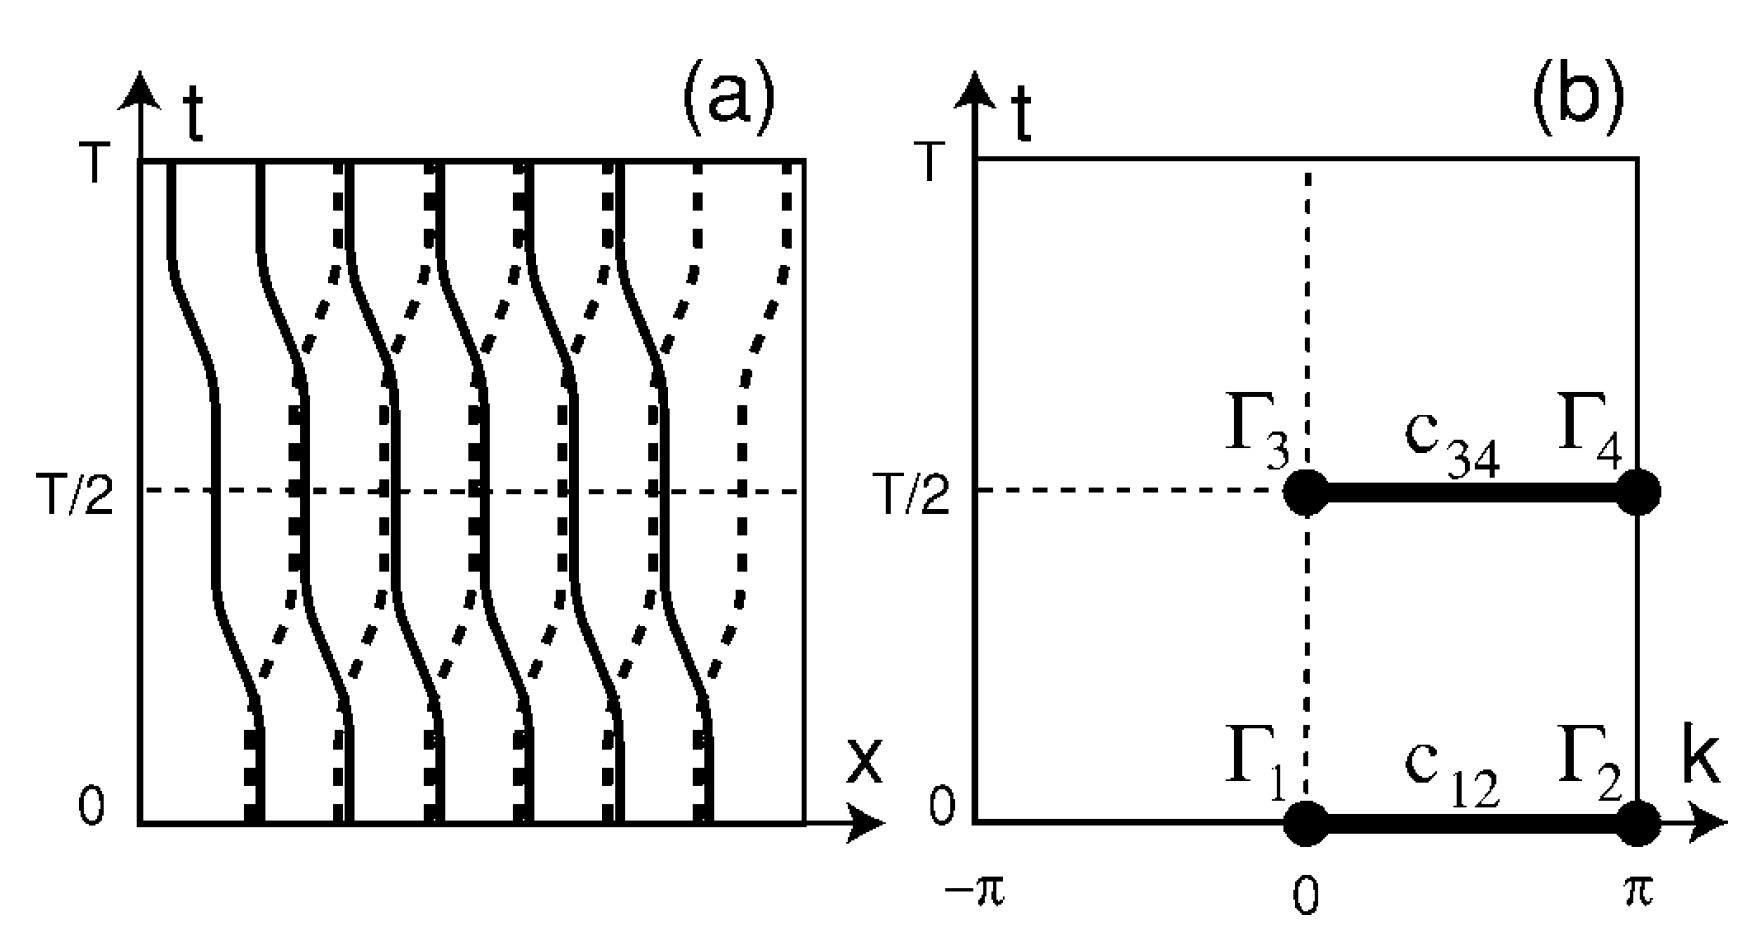
\includegraphics[height=2in]{Fu-Kane.png}
    \caption{(a)图表示Wannier态时间反演对中心的演化,在$t=0,t=T/2$之间,Wannier态交换配对伙伴,结果导致末端出现未配对的Wannier态。(b)由$k-t$定义的环面}
\end{figure}
之前的$Fu-Kane$自旋pump中,从$t=0$到$t=\frac{T}{2}$过程中,Wannier态交换成对。在这个过程中,时间反演极化率改变$1$. 此外,这个交换导致了在每一个末端出现未配对的Wannier占据态。由于Wannier态是成对出现的,因此每一端必定有两个Kramers简并度,从而导致总简并度为4。

当系统从$t= t /2$演变到$t$时,又出现了另一个交换,时间反转极化恢复到原来的值。然而由于$H(t)=\Theta H(T-t)\Theta^{-1}$,两端开的系统在$t$时刻不会回到原来的状态,但由于$t= t /2$处的能级交叉,其末端处于激发态。

我们现在把这个非平凡pump循环的出现与作为t的函数的体态基态的拓扑性质联系起来。我们考虑时间反演极化率在$t=0$到$T/2$的变化。注意,虽然$P_{\Theta}$不是规范不变的,但是$P_{\theta}$的变化量是规范不变的。差值:
\begin{equation}
    \Delta=[P_\theta(T/2)-P_\theta(0)]\mod{2}
\end{equation}
定义了$Z_2$拓扑不变量,用来表征由$k$和$t$定义的$T^2$流形到波函数$|u_n(k,t)\rangle$的映射。从TR极化率表达式$P_\theta$可以得到这个不变量为
\begin{equation}
    (-1)^\Delta=\prod_{i=1}^{4}\frac{\sqrt{\det[w(\Gamma_i)]}}{Pf[w(\Gamma_i)]}
\end{equation}
这里$\Gamma_i$是四个TRIM点。通过沿着路径$c_{12}$和$c_{34}$连续演化$\sqrt{\det[w(k,t)]}$,选择平方根的分支为$P_\theta$表达式所写。为了应用这个公式,在环面上连续定义波函数是至关重要的。通过$U(2N)$变换($|u_n\rangle=\sum_{m}U_{nm}(k)|u_{m}(k)\rangle$)总是能找到这样光滑定义的波函数,因为Chern数为$0$. 

如果一个绝缘体有附加的反演对称性,那么存在一个简单的导数方法去计算$Z_2$不变。假设哈密顿$H$满足反演不变
\begin{equation}
    H(-k)=PH(k)P^{-1}
\end{equation}
其中宇称算符定义为
\begin{equation}
    P|r,s_z\rangle=P|-r,s_z\rangle
\end{equation}
这里由于$r$是坐标,$s_z$是赝矢量,结合TR对称和P对称的一个显然的结果是Berry曲率为$0$:
\begin{equation}
    F(k)=\nabla_k\times A(k)=0
\end{equation}
具体证明可以参考Bernevig第四章最后一段,简单来说,根据Berry曲率的定义,在时间反演下$F(-k)=-F(k)$,在空间反演下$F(-k)=F(k)$. 考虑在TRIM点$\Gamma_i$的第$m$对占据能带,我们定义$P|u_{2m,\Gamma_i}\rangle=\xi_{2m}(\Gamma_i)|u_{2m,\Gamma_i}\rangle$其中宇称本征值$\xi_{2m}(\Gamma_i)=+1,-1$. 简并的Kramers对共同拥有相同的本征值$\xi_{2m}=\xi_{2m-1}$\footnote{对于Kramers对$|u_{2m}(\Gamma_i)\rangle$和$|u_{2m+1}(\Gamma_i)=\Theta|u_{2m}(\Gamma_i)\rangle$\\由于$[P,\Theta]=0,$,所以有$P|u_{2m}(\Gamma_i)\rangle=\xi_{2m}(\Gamma_i)|u_{2m}(\Gamma_i)\rangle$和$P|u_{2m+1}(\Gamma_i)\rangle=P\Theta|u_{2m}(\Gamma_i)\rangle=\xi_{2m}(\Gamma_i)|u_{2m=1}(\Gamma_i)\rangle$. 此即一对Kramers对的空间反演本征值一样}. 在这个情况下,有一个简单公式去计算$\delta$
\begin{equation}
    (-1)^{\nu}=\prod_{i}\prod_{m=1}^{N}\xi_{2m}(\Gamma_i)
\end{equation}
\subsubsection*{$Z^2$与Berry曲率的关系}
PHYSICAL REVIEW B 74, 195312 (2006)附录部分

\subsection{二维或三维的推广}
从二维$Z_2$推广到三维$Z_2$是一件里程碑的事情。拓扑不变量表征了二维带结构可以通过将二维系统卷成圆柱来构建。通过圆柱的磁通扮演一个圆周晶格动量$k_x$的角色,其中$\phi=0$和$\phi=\frac{\phi_0}{2}$对应于两个边缘时间反演动量$k_x=\Lambda_1=0$和$k_x=\Lambda_2=\frac{\pi}{a}$. $Z_2$不变量表征了在$k_x=\Lambda_1$和$k_x=\Lambda_2$之间一维系统末端Kramers简并中的时间反演极化。对于二维周期边界的系统,这个改变与体态带结构有关。对于方格子,FBZ中四个TRIM点分别是
\begin{equation}
    \Gamma_{n_x,n_y}=\left(\frac{n_x}{2}G_x,\frac{n_y}{2}G_y\right)
\end{equation}
其中$n_x,n_y=0,1$. 对于与$G_y$垂直的边缘,一维边缘时间反演不变动量点事$k_x=\Lambda_1$和$k_x=\Lambda_2$,满足$\Gamma_{1,n_y}-\Gamma_{0,n_y}=\frac{G_x}{2}$. 这样,时间反演极化可以表示成$\pi_x=\delta_{x1}\delta_{x2}$,其中
\begin{equation}
    \delta_{xi}=\frac{\sqrt{det[w(\Gamma_{i,y})]}}{Pf[w(\Gamma_{i,y})]}=\pm1
\end{equation}
上式表示对于垂直$k_y$方向的TRIM点计算。$\pi_x$并不是规范不变的,依赖于$k$的规范可以改变任意对$\delta_i$的符号。如果我们把这个系统沿着另一个方向卷成圆柱,我们可以得到时间反演极化$\pi_y=\delta_{y1}\delta_{y2}$. 他们的乘积是规范不变的:
\begin{equation}
    (-1)^\nu=\prod_{n_x,n_y=0,1}\frac{\sqrt{det[w(\Gamma_{n_x,n_y})]}}{Pf[w(\Gamma_{n_x,n_y})]}
\end{equation}
这个$\nu$可以等于$0,1$,并且定义了一个单独的二维$Z_2$不变量。对于三维晶格的$Z_2$不变量可以化简到二维情况里。三维布里渊区可以沿着$x,y$卷成甜甜圈。对于三维情况,有八个TRIM点:
\begin{equation}
    \Gamma_{i=(n_1,n_2,n_3)}=\left(\frac{n_1}{2}G_1,\frac{n_2}{2}G_2,\frac{n_3}{2}G_3\right)
\end{equation}
其中$n_j=0,1$. 他们可以被看做平行六面体的八个顶角。对于固定的$n_1$,例如$n_1=1$,点集合为
\begin{equation}
    \left(\frac{n_1}{2}G_1,\frac{a_2}{2}G_2,\frac{a_3}{2}G_3\right)
\end{equation}
对于所有$a_1,a_3\in[-\frac{1}{2},\frac{1}{2})$定义了一个二维系统对应时间反演对称性的二维布里渊区,其中$Z_2$不变量可以用二维系统的方法计算,被称为$\nu_{n_1=1}$. 其余五个不变量$\nu_{n_1=0},\nu_{n_2=0,1}$和$\nu_{n_3=0,1}$可以用相似的方法来定义。这六个不变量由平行六面体的六个面联系起来。因为他们属于相同的三维晶格,仅仅只有四个是独立的。这是由于约束条件:
\begin{equation}
    \nu_{n_1}\cdot\nu_{n_1=1}=\nu_{n_2=0}\cdot\nu_{n_2=1}=\nu_{n_3=0}\cdot\nu_{n_3=1}\mathrm{mod}2
\end{equation}
这个四个独立不变量可以被选定为$\nu_{0}=\nu_{n_1=0}\nu_{n_1=1},\nu_1=\nu_{n_1=1},\nu_2=\nu_{n_2=1},\nu_{3}=\nu_{n_3=1}$. 这个指标$\nu_0;(\nu_1,\nu_2,\nu_3)$反应了表面态的拓扑。$\nu_0$由下式给出
\begin{equation}
    (-1)^{\nu_0}=\prod_{n_1,n_2,n_3}\frac{\sqrt{\det[w(\Gamma_{n_1,n_2,n_3})]}}{Pf[w(\Gamma_{n_1,n_2,n_3})]}
\end{equation}
如果$\nu_0=1$,那么这个系统是一个强拓扑绝缘体,在晶格的所有表面上伴随着奇数个狄拉克cone。如果$\nu_0=1$,那么晶格是一个弱拓扑绝缘体,伴随着表面上有偶数个狄拉克cone。后者拓扑等价于一个二维绝缘体并且因此没有对无序的Robust. 举个例子$0;(0,0,1)$,这个表面态对应于由$G_2$和$G_3$生成的二维布里渊区有两个狄拉克cones$(\nu_1=0)$,并且对于在由$G_1$和$G_3$生成的布里渊区中有相同的表面态$(\nu_2=0)$. 但是在$G_2-G_3$平面上没有表面态$(\nu_3=1)$
\subsection{修正狄拉克方程的相图}
我们先考虑修正狄拉克方程是否拓扑平凡或者拓扑不平凡。对于一个无穷系统或者周期性边界条件而言,波函数的一般解可以表示成
\begin{equation}
    \Psi_\nu=u_\nu(\mathbf{p})e^{\frac{i}{\hbar}(\mathbf{p}\cdot\mathbf{r}-E_{p,\nu}t)}
\end{equation}
对于平面波解而言,动量是一个好量子数。四条能带的色散关系为
\begin{equation}
    E_{p,\nu=1,2}=\sqrt{v^2p^2+(mv^2-B\mathbf{p}^2)^2}
\end{equation}
\begin{equation}
    E_{p,\nu=3,4}=-\sqrt{v^2p^2+(mv^2-B\mathbf{p}^2)^2}
\end{equation}
四分量旋量$u_\nu(\mathbf{p})$可以表示成$u_\nu(\mathbf{p})=\Lambda_{\frac{1}{2}}u_{\nu}(\mathbf{p}=0)$. 其中$\Lambda_{\frac{1}{2}}$为
\begin{equation}
    \Lambda_{\frac{1}{2}}=\begin{pmatrix}
        \cosh\frac{\rho}{2}&\mathbf{n}\cdot\mathbf{\sigma}\sinh\frac{\rho}{2}\\
        \mathbf{n}\cdot\mathbf{\sigma}\sinh\frac{\rho}{2}&\cosh\frac{\rho}{2}
    \end{pmatrix}
\end{equation}
所以得到Boost矩阵
\begin{equation}
    \Lambda_{\frac{1}{2}}=\sqrt{\frac{\epsilon_p}{2E_{p,1}}}\begin{pmatrix}
        I&-\frac{v\mathbf{p}}{\epsilon_p}\cdot\mathbf{\sigma}\\
        \frac{v\mathbf{p}}{\epsilon_p}\cdot\mathbf{\sigma}&I
    \end{pmatrix}
\end{equation}
其中$\epsilon_p=E_{p,1}+(mv^2-B\mathbf{p}^2)$. 当$\mathbf{p}=0$时,狄拉克方程的解为
\begin{equation}
    \begin{split}
        Hu_{\nu}(p=0)&=Eu_{\nu}(p=0)\Rightarrow E_{p,\nu=1,2}=-E_{p,\nu=3,4}=mv^2,\\
        u_{1}(p=0)&=\begin{pmatrix}
            1\\0\\0\\0
        \end{pmatrix},u_2(p=0)=\begin{pmatrix}
            0\\1\\0\\0
        \end{pmatrix},u_3(p=0)=\begin{pmatrix}
            0\\0\\1\\0
        \end{pmatrix},u_4(p=0)=\begin{pmatrix}
            0\\0\\0\\1
        \end{pmatrix}
    \end{split}
\end{equation}
所以得到
\begin{equation}
    u_{\nu}(\mathbf{p})=\sqrt{\frac{\epsilon_p}{2E_{p,1}}}\begin{pmatrix}
        1&0&-\frac{p_zv}{\epsilon_p}&-\frac{p_-v}{\epsilon_p}\\
        0&1&-\frac{p_+v}{\epsilon_p}&\frac{p_zv}{\epsilon_p}\\
        \frac{p_zv}{\epsilon_p}&\frac{p_-v}{\epsilon_p}&1&0\\
        \frac{p_+v}{\epsilon_p}&-\frac{p_zv}{\epsilon_p}&0&1
    \end{pmatrix}u_\nu(\mathbf{p}=0)
\end{equation}
修正狄拉克方程的拓扑性质可以通过获得的这些解得到。
\begin{equation}
    \begin{split}
        u_1(\p)=\sqrt{\frac{\epsilon_p}{2E_{p,1}}}\begin{pmatrix}
            1\\
            0\\
            \frac{p_zv}{\epsilon_p}\\
            \frac{p_+v}{\epsilon_{p}}
        \end{pmatrix}
    \end{split},u_2(\p)=\sqrt{\frac{\epsilon_p}{2E_{p,1}}}\begin{pmatrix}
        0\\
        1\\
        \frac{p_-v}{\epsilon_p}\\
        -\frac{p_zv}{\epsilon_p}
    \end{pmatrix},u_3(\p)=\sqrt{\frac{\epsilon_p}{2E_{p,1}}}\begin{pmatrix}
        -\frac{p_zv}{\epsilon_p}\\
        -\frac{p_+v}{\epsilon_p}\\
        1\\
        0
    \end{pmatrix},u_4(\p)=\sqrt{\frac{\epsilon_p}{2E_{p,1}}}\begin{pmatrix}
        -\frac{p_-v}{\epsilon_p}\\
        \frac{p_zv}{\epsilon_p}\\
        0\\
        1
    \end{pmatrix}
\end{equation}
狄拉克方程在时间反演下不变,并且可以通过$Z_2$拓扑分类来分类。
\begin{equation}
    H=v\alpha\cdot\mathbf{p}+(mv^2-Bp^2)\beta
\end{equation}
这里讨论一下狄拉克表示下的时间反演算符的表示矩阵:

在量子场论里狄拉克方程为
\begin{equation}
    (i\slashed{\partial}-m)\psi(x)=0
\end{equation}
量子化解为
\begin{equation}
    \psi(x)=\int\frac{\mathrm{d}^3x}{(2\pi)^3}\frac{1}{\sqrt{2E_{\mathbf{p}}}}\sum_{s}\left(a_p^su^s(p)e^{-\frac{i}{\hbar}p\cdot x}+b_p^{s\dagger}v^s(p)e^{\frac{i}{\hbar}p\cdot x}\right)
\end{equation}
$\psi(x)$架设表示空间,时间反演算符作用上去得到线性表示:
\begin{equation}
    \Theta\psi(x)\Theta^{-1}=\int\frac{\dd[3]x}{(2\pi)^3}\frac{1}{\sqrt{E_{p}}}\sum_{s}\left(a_{-p}^{-s}[u^s(p)]^*e^{\frac{i}{\hbar}p\cdot x}+b_{-p}^{-s^\dagger}[v^{s}(p)]^*e^{-\frac{i}{\hbar}p\cdot x}\right)
\end{equation}
对于$u^s(p)$而言
\begin{equation}
    u^{s}(p)=\begin{pmatrix}
        \sqrt{p\cdot\sigma}\xi^s\\
        \sqrt{p\cdot\bar{\sigma}}\xi^s
    \end{pmatrix}
\end{equation}
$\xi^s$是二分量旋量,我们定义$\xi^{-s}=-i\sigma^2(\xi^s)^*$为该二分量旋量的时间反演对应的旋量。$\xi^s=(\xi(\uparrow),\xi(\downarrow))$,其中
\begin{equation}
    \xi(\uparrow)=\begin{pmatrix}
        \cos\frac{\theta}{2}\\
        e^{i\phi}\sin{\frac{\theta}{2}}
    \end{pmatrix},\quad\xi(\downarrow)=\begin{pmatrix}
        -e^{-i\phi\sin\frac{\theta}{2}}\\
        \cos\frac{\theta}{2}
    \end{pmatrix}
\end{equation}
显然,可以得到:
\begin{equation}
    \xi^{-s}=(\xi(\downarrow),-\xi(\uparrow)),\quad a_p^{-s}=(a_p^2,-a_p^1),\quad b_p^{-s}=(b_p^2,-b_p^1)
\end{equation}
定义$\tilde{p}=(p^0,-\mathbf{p})$利用等式:$\mathbf{\sigma}\sigma^2=\sigma^2(-\mathbf{\sigma}^*)$我们得到
\begin{equation}
    \begin{split}
        u^{-s}(\tilde{p})&=\begin{pmatrix}
            \sqrt{\tilde{p}\cdot\sigma}\xi^{-s}\\
            \sqrt{\tilde{p}\cdot\bar{\sigma}}\xi^{-s}
        \end{pmatrix}=\begin{pmatrix}
            \sqrt{\tilde{p}\cdot\sigma}(-i\sigma^2)(\xi^s)^*\\
            \sqrt{\tilde{p}\cdot\bar{\sigma}}(-i\sigma^2)(\xi^s)^*
        \end{pmatrix}=\begin{pmatrix}
            (-i\sigma^2)\sqrt{p\cdot\sigma^*}(\xi^s)^*\\
            (-i\sigma^2)\sqrt{p\cdot\bar{\sigma}^*}(\xi^s)^*
        \end{pmatrix}\\
        &=-i\begin{pmatrix}
            \sigma^2&0\\
            0&\sigma^2
        \end{pmatrix}[u^s(p)]^*=-\gamma^1\gamma^3[u^s(p)]^*
    \end{split}
\end{equation}
同理对于反粒子的旋量
\begin{equation}
    v^s(p)=\begin{pmatrix}
        \sqrt{p\cdot\sigma}\xi^{-s}\\
        -\sqrt{p\cdot\bar{\sigma}}\xi^{-s}
    \end{pmatrix}
\end{equation}
作用于时间反演后同样的我们得到:
\begin{equation}
    v^{-s}(\tilde{p})=-\gamma^1\gamma^3[v^s(p)]^*
\end{equation}
上面关系式带入费米场算符里得到狄拉克场架设表示空间里的时间反演算符的表示矩阵:
\begin{equation}
    \begin{split}
        \Theta\psi(x)\Theta^{-1}&=\int\frac{\mathrm{d}^3x}{(2\pi)^3}\frac{1}{\sqrt{E_{p}}}\sum_{s}\left(a_{-p}^{-s}[u^s(p)]^*e^{\frac{i}{\hbar}p\cdot x}+b_{-p}^{-s^\dagger}[v^{s}(p)]^*e^{-\frac{i}{\hbar}p\cdot x}\right)\\
        &=\int\frac{\mathrm{d}^3x}{(2\pi)^3}\frac{1}{\sqrt{E_{\tilde{p}}}}\sum_{s}\left(a_{\tilde{p}}^{-s}(\gamma^1\gamma^3)u^{-s}(\tilde{p})e^{\frac{i}{\hbar}\tilde{p}\cdot(t,-\mathbf{x})}+b_{\tilde{p}}^{-s}(\gamma^1\gamma^3)v^{-s}(\tilde{p})e^{-\frac{i}{\hbar}\tilde{p}\cdot(t,-\mathbf{x})}\right)\\
        &=\gamma^1\gamma^3\int\frac{\mathrm{d}^3x}{(2\pi)^3}\frac{1}{\sqrt{E_{\tilde{p}}}}\sum_{s}\left(a_{\tilde{p}}^{-s}u^{-s}(\tilde{p})e^{i\tilde{p}(t,-\mathbf{x})}+b_{\tilde{p}}^{s\dagger}v^{-s}(\tilde{p})e^{-ip(t,-\mathbf{x})}\right)\\
        &=\gamma^1\gamma^3\psi(-t,\mathbf{x})
    \end{split}
\end{equation}
我们知道$\alpha^i=\gamma^0\gamma^i$,所以$\gamma^1\gamma^3=-\alpha^1\alpha^3$. 时间反演算符可以写成$\Theta=T\mathcal{K}$. 考虑到时间反演算符的复共轭算子,如下定义时间反演算符是合理的
\begin{equation}
    \Theta=-i\alpha_x\alpha_z\mathcal{K}
\end{equation}
$\mathcal{K}$是复共轭算符,该算符作用在右矢量上或者波函数上让右矢系数或者波函数系数取复共轭。修正狄拉克方程在时间反演下仍然是不变的
\begin{equation}
    \begin{split}
        \Theta\alpha_x\Theta^{-1}&=-i\alpha_x\alpha_z\mathcal{K}\alpha_xi\alpha_x\alpha_z\mathcal{K}=-\alpha_x\\
        \Theta\alpha_y\Theta^{-1}&=-i\alpha_x\alpha_z\mathcal{K}\alpha_yi\alpha_x\alpha_z\mathcal{K}=-\alpha_y\quad\Rightarrow\Theta\mathbf{\alpha}\Theta^{-1}=-\mathbf{\alpha}\\
        \Theta\alpha_z\Theta^{-1}&=-i\alpha_x\alpha_z\mathcal{K}\alpha_zi\alpha_x\alpha_z\mathcal{K}=-\alpha_z
    \end{split}
\end{equation}
修正狄拉克方程哈密顿
\begin{equation}
    H=v\alpha\cdot\mathbf{p}+(mv^2-Bp^2)\beta
\end{equation}
满足时间反演对称性:$\Theta H(p)\Theta^{-1}=H(-p)$

$p$是一个好量子数。进一步说,我们有时间反演关系
\begin{equation}
    \Theta u_1(\mathbf{p})=-iu_2(-\mathbf{p}),\quad\Theta u_2(\p)=iu_1(-\p)
\end{equation}
\begin{equation}
    \Theta u_3(\p)=-iu_4(-\p),\quad\Theta u_4(\p)=iu_3(-\p)
\end{equation}
\textcolor{red}{值得注意,量子场论里时间反演算符表示矩阵为$-\gamma^1\gamma^3$
\begin{equation}
    -\gamma^1\gamma^3=-\begin{pmatrix}
        \quad&\sigma^1\\
        -\sigma^1&\quad
    \end{pmatrix}\begin{pmatrix}
        \quad&\sigma^3\\
        -\sigma^3&\quad
    \end{pmatrix}=-i\begin{pmatrix}
        \sigma^2&\quad\\
        \quad&\sigma^2
    \end{pmatrix}
\end{equation}
\begin{equation}
    u^{-s}(t,-\p)=-\gamma^1\gamma^3[u^s(t,\p)]^*\Rightarrow u^s(t,\p)=\gamma^1\gamma^3[u^s(t,-\p)]^*
\end{equation}
也就是说:
\begin{equation}
    \gamma^1\gamma^3 u_1(\p)=-u_2(-\p),\gamma^1\gamma^3u_2(p)=u_1(p)
\end{equation}
对应到凝聚态里多了一个$i$系数
\begin{equation}
    \Theta=i\gamma^1\gamma^3\mathcal{K}
\end{equation}
所以有反演关系
\begin{equation}
    \Theta u_1(\mathbf{p})=-iu_2(-\mathbf{p}),\quad\Theta u_2(\p)=iu_1(-\p)
\end{equation}
\begin{equation}
    \Theta u_3(\p)=-iu_4(-\p),\quad\Theta u_4(\p)=iu_3(-\p)
\end{equation}
}
这样$\{u_1(\p),u_2(-\p)\}$和$\{u_3(\p),u_4(\p)\}$分别是正能和负能的二重简并的Kramers对。矩阵$\langle u_\mu(\p)|\Theta|u_\nu(\p)\rangle$为
\begin{equation}
    \langle u_1(\p)|\Theta|u_2(\p)\rangle=i\langle u_1(\p)|u_1(-p)\rangle=i\frac{\epsilon_p}{2E_{p,1}}(1-\frac{p_z^2v^2}{\epsilon_p^2}-\frac{|p_+|^2v^2}{\epsilon_p^2})=i\frac{\epsilon_p}{2E_{p,1}}(1-\frac{p^2v^2}{\epsilon_p^2})=i\frac{mv^2-Bp^2}{E_{p,1}}
\end{equation}
\begin{equation}
    \langle u_1(\p)|\Theta|u_3(\p)\rangle=-i\langle u_1(\p)|u_4(-\p)\rangle=-i\frac{p_-v}{E_{p,1}}
\end{equation}
\begin{equation}
    \langle u_1(\p)|\Theta|u_4(\p)\rangle=i\langle u_1(\p)|u_3(-\p)\rangle=i\frac{p_zv}{E_{p,1}}
\end{equation}
\begin{equation}
    \langle u_2(\p)|\Theta|u_3(\p)\rangle=-i\langle u_2(\p)|u_4(-\p)\rangle=i\frac{p_zv}{E_{p,1}}
\end{equation}
\begin{equation}
    \langle u_2(\p)|\Theta|u_4(\p)\rangle=i\langle u_2(\p)|u_3(-\p)\rangle=i\frac{p_+v}{E_{p,1}}
\end{equation}
\begin{equation}
    \langle u_3(\p)|\Theta|u_4(p)\rangle=i\langle u_3(\p)|u_3(-\p)\rangle=i\frac{mv^2-Bp^2}{E_{p,1}}
\end{equation}
其余的矩阵元由于Kramers简并,相互正交而为$0$. 考虑到时间反演算符的性质$\Theta^2=1$得到矩阵元满足关系式:
\begin{equation}
    \langle u_\mu(\p)|\Theta|u_\nu(p)\rangle=-\langle\Theta^2u_\mu(\p)|\Theta|u_\nu(\p)\rangle=-\langle u_\nu(\p)|\Theta|u_\mu(\p)
\end{equation}
所以交叠矩阵是一个反对称矩阵,对角元为$0$. 以上所有矩阵元是所有的独立矩阵元,可以写出
\begin{equation}
    w_{\mu\nu}=\begin{pmatrix}
        0&i\frac{mv^2-Bp^2}{E_{p,1}}&-i\frac{p_-v}{E_{p,1}}&i\frac{p_zv}{E_{p,1}}\\
        -i\frac{mv^2-Bp^2}{E_{p,1}}&0&i\frac{pzv}{E_{p,1}}&i\frac{p_+v}{E_{p,1}}\\
        i\frac{p_-v}{E_{p,1}}&-i\frac{p_zv}{E_{p,1}}&0&i\frac{mv^2-Bp^2}{E_{p,1}}\\
        -i\frac{p_zv}{E_{p,1}}&-i\frac{p_+v}{E_{p,1}}&-i\frac{mv^2-Bp^2}{E_{p,1}}&0
    \end{pmatrix}
\end{equation}
在绝缘体中对于两条满占据的负能带$u_3(\p)$和$u_4(-\p)$,交叠矩阵的子矩阵可以用一个单独的数来表出$\epsilon_{\mu\nu}P(\p)$
\begin{equation}
    P(\p)=i\frac{mv^2-Bp^2}{\sqrt{v^2p^2+(mv^2-Bp^2)^2}}
\end{equation}
这就是$2\times2$矩阵的Pfaffian. 偶数或者奇数个$P(\p)$的零定义了$Z_2$拓扑不变量。这里我们想要强调无量纲参数$mB$会决定修正狄拉克方程的$Z_2$不变量。因为对于$mB<0$,$P(\p)$总是非零的,并且Pfaffian不存在零,我们立即可以得出结论,对于$mB\leq0$的修正狄拉克方程(包括$B=0$)是拓扑平凡的。

对于$mB>0$的情况是不同的。在连续模型里,布里渊区变成无穷大。在$\p=0$和$\p=+\infty$处,$P(0)=i\mathrm{sgn}(m),P(+\infty)=-\mathrm{sgn}(B)$. 在这个情况下,在$p^2=\frac{mv^2}{B}$处$P(p)=0$. $\p=0$总是一个TRIM点。作为一个动量空间中的各向同性模型的结果,如果我们把连续模型看成通过让$a\to0$倒格矢$G=\frac{2\pi}{a}\to\infty$格点模型的极限,我们可以认为所有$p=+\infty$的点都收缩到一个点上。从这个意义上说,作为方晶格的极限,如果$mB>0$,另外三个TRIM点$P(0,\frac{G}{2})=P(\frac{G}{2},0)=P(\frac{G}{2},\frac{G}{2})=P(+\infty)$符号与$P(0)$相反。对于立方晶格也类似,其他七个TRIM点的$P(\p)$也和$P(0)$异号。正如Fu,Kane在文献中所说,我们得出结论,当且仅当$mB>0$,修正狄拉克哈密顿是拓扑非平凡的。

在二维情况,$Z_2$指标也可以通过在$\p=p_x+ip_y$的复平面沿着半布里渊区计算$P(\p)$相位的Winding number来决定:
\begin{equation}
    I=\frac{1}{2\pi i}\oint_C\md\p\cdot\nabla_{\p}log[P(\p)+i\delta]
\end{equation}
由于模型是各向同性的,$\delta>0,|\p|\to+\infty$半圆部分的积分为$0$,积分可以被化简到仅仅沿着$p_x$轴的路径。当$mB>0$时沿着$p_x$在环中的一对零点被围道$C$包围,这给出$\nu=1$的$Z_2$指数。这定义了非平凡量子自旋霍尔效应。

Volovok提出了用格林函数而不是哈密顿来分类拓扑绝缘体。对于三维狄拉克方程,格林函数有形式:
\begin{equation}
    \begin{split}
        G(i\omega,\p)&=\frac{1}{i\omega_n-H}\\
        &=-\frac{i\omega_n+v\alpha\cdot\p+(mv^2-Bp^2)\beta}{\omega_n^2+h^2(p)}
    \end{split}
\end{equation}
其中$h(k)=H^2=v^2p^2+(mv^2-Bp^2)^2$. 频率$\omega_n=\frac{(2n+1)\pi}{\beta}$. 拓扑不变量定义为
\begin{equation}
    N=\frac{1}{24\pi^2}\epsilon_{ijk}Tr[K\int_{i\omega_n=0}\md\p G\partial_{p_i}G^{-1}G\partial_{p_j}G^{-1}G\partial_{p_k}G^{-1}]
\end{equation}
其中$K=\sigma_y\otimes\sigma_0$是对称算符。最后结果为:
\begin{equation}
    N=\mathrm{sgn}(m)+\mathrm{sgn}(B)
\end{equation}
当$mB>0$时,$N=\pm2$,这定义了拓扑非平凡相。如果$B>0$,存在从$m<0$的拓扑平凡相到$m>0$的拓扑非平凡相。这与$Z_2$指标的结果一致。相图如下
\begin{center}
    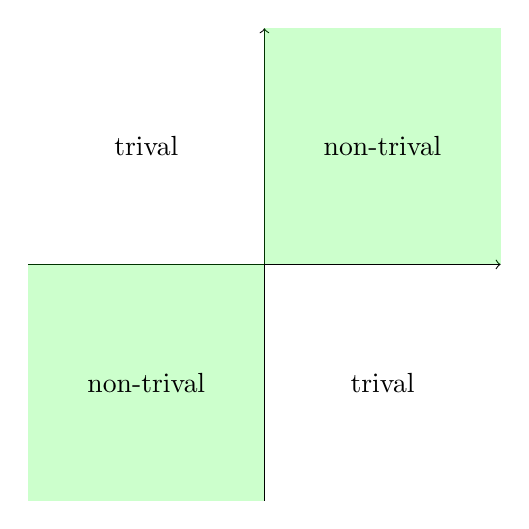
\begin{tikzpicture}
        \draw[->] (-3,0) -- (3,0);
        \draw[->] (0,-3) -- (0,3);
        \fill[green,opacity=0.2] (0,0) rectangle (3,3);
        \fill[green,opacity=0.2] (0,0) rectangle (-3,-3);
        \node at (-1.5,1.5) {trival};
        \node at (-1.5,-1.5) {non-trival};
        \node at (1.5,-1.5) {trival};
        \node at (1.5,1.5) {non-trival};
    \end{tikzpicture}
\end{center}
\section{一维拓扑相}
\subsection{SSH模型}
最简单的二带模型是聚乙炔的SSH模型,它是一个有手征对称性的绝缘体。考虑一维二聚体晶格
\begin{equation}
    H=\sum_{n=1}^{N}(t+\delta t)c_{A,n}^\dagger c_{B,n}+\sum_{n=1}^N(t-\delta t)c_{A,n+1}^\dagger c_{B,n}+h.c.
\end{equation}
其中$c_{A(B),n}^\dagger$和$c_{A(B),n}$是在A(B)子格格点(A(B),n)上的电子产生湮灭算符。在这个模型里,每一个原胞包含两个格点,$A$和$B$,hopping项连接了两个不同子格格点。原胞内hopping振幅是$t+\delta t$并且两个原胞间的hopping为$t-\delta t$. 有两个明显的相,A和B相,如图所示。这两个相被认为是简并的。这两相的界面形成域壁,域壁附近可能产生孤子解。在本节中,我们将说明在开边界条件下,这两个阶段在拓扑上是不同的。
\begin{center}
    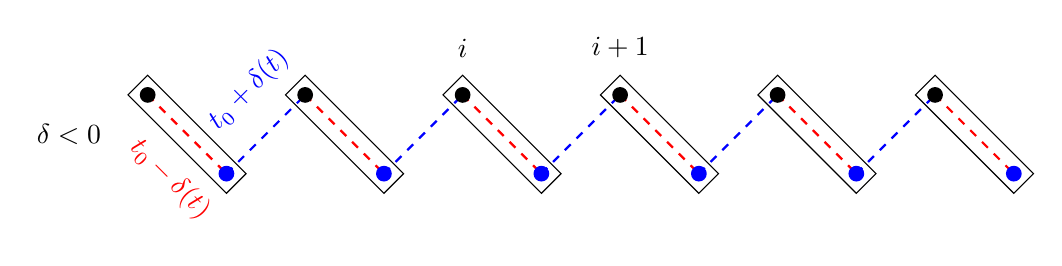
\begin{tikzpicture}
        \draw (-0.25,0) -- (1,-1.25) -- (1.25,-1) -- (0,0.25) -- cycle;
        \draw (1.75,0) -- (3,-1.25) -- (3.25,-1) -- (2,0.25) -- cycle;
        \draw (3.75,0) -- (5,-1.25) -- (5.25,-1) -- (4,0.25) -- cycle;
        \draw (5.75,0) -- (7,-1.25) -- (7.25,-1) -- (6,0.25) -- cycle;
        \draw (7.75,0) -- (9,-1.25) -- (9.25,-1) -- (8,0.25) -- cycle;
        \draw (9.75,0) -- (11,-1.25) -- (11.25,-1) -- (10,0.25) -- cycle;
        \draw[dashed,thick,red] (0,0) --node[below=1em,rotate=-45]{$t_0-\delta(t)$} (1,-1);
        \draw[dashed,thick,red] (2,0) -- (3,-1);
        \draw[dashed,thick,red] (4,0) -- (5,-1);
        \draw[dashed,thick,red] (6,0) -- (7,-1);
        \draw[dashed,thick,red] (8,0) -- (9,-1);
        \draw[dashed,thick,red] (10,0) -- (11,-1);
        \draw[dashed,thick,blue] (1,-1) --node[above=1em,rotate=45]{$t_0+\delta(t)$} (2,0);
        \draw[dashed,thick,blue] (3,-1) -- (4,0);
        \draw[dashed,thick,blue] (5,-1) -- (6,0);
        \draw[dashed,thick,blue] (7,-1) -- (8,0);
        \draw[dashed,thick,blue] (9,-1) -- (10,0);
        \fill (0,0) circle (0.1);
        \fill (2,0) circle (0.1);
        \fill (4,0)node[above=1em]{$i$} circle (0.1);
        \fill (6,0)node[above=1em]{$i+1$} circle (0.1);
        \fill (8,0) circle (0.1);
        \fill (10,0) circle (0.1);
        \fill[blue] (1,-1) circle (0.1);
        \fill[blue] (3,-1) circle (0.1);
        \fill[blue] (5,-1) circle (0.1);
        \fill[blue] (7,-1) circle (0.1);
        \fill[blue] (9,-1) circle (0.1);
        \fill[blue] (11,-1) circle (0.1);
        \node at (-1,-0.5) {$\delta<0$};
    \end{tikzpicture}
\end{center}
\begin{center}
    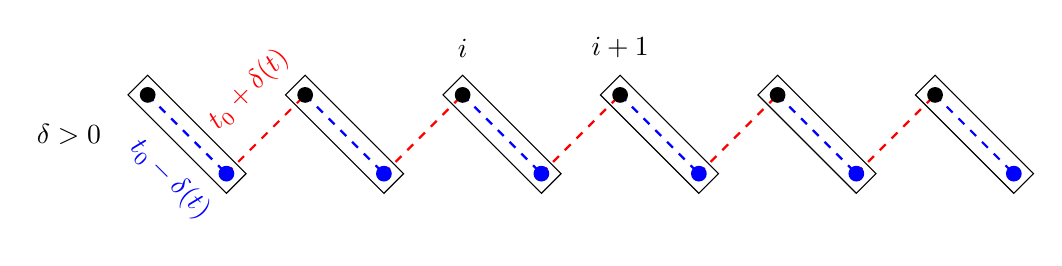
\begin{tikzpicture}
        \draw (-0.25,0) -- (1,-1.25) -- (1.25,-1) -- (0,0.25) -- cycle;
        \draw (1.75,0) -- (3,-1.25) -- (3.25,-1) -- (2,0.25) -- cycle;
        \draw (3.75,0) -- (5,-1.25) -- (5.25,-1) -- (4,0.25) -- cycle;
        \draw (5.75,0) -- (7,-1.25) -- (7.25,-1) -- (6,0.25) -- cycle;
        \draw (7.75,0) -- (9,-1.25) -- (9.25,-1) -- (8,0.25) -- cycle;
        \draw (9.75,0) -- (11,-1.25) -- (11.25,-1) -- (10,0.25) -- cycle;
        \draw[dashed,thick,blue] (0,0) --node[below=1em,rotate=-45]{$t_0-\delta(t)$} (1,-1);
        \draw[dashed,thick,blue] (2,0) -- (3,-1);
        \draw[dashed,thick,blue] (4,0) -- (5,-1);
        \draw[dashed,thick,blue] (6,0) -- (7,-1);
        \draw[dashed,thick,blue] (8,0) -- (9,-1);
        \draw[dashed,thick,blue] (10,0) -- (11,-1);
        \draw[dashed,thick,red] (1,-1) --node[above=1em,rotate=45]{$t_0+\delta(t)$} (2,0);
        \draw[dashed,thick,red] (3,-1) -- (4,0);
        \draw[dashed,thick,red] (5,-1) -- (6,0);
        \draw[dashed,thick,red] (7,-1) -- (8,0);
        \draw[dashed,thick,red] (9,-1) -- (10,0);
        \fill (0,0) circle (0.1);
        \fill (2,0) circle (0.1);
        \fill (4,0)node[above=1em]{$i$} circle (0.1);
        \fill (6,0)node[above=1em]{$i+1$} circle (0.1);
        \fill (8,0) circle (0.1);
        \fill (10,0) circle (0.1);
        \fill[blue] (1,-1) circle (0.1);
        \fill[blue] (3,-1) circle (0.1);
        \fill[blue] (5,-1) circle (0.1);
        \fill[blue] (7,-1) circle (0.1);
        \fill[blue] (9,-1) circle (0.1);
        \fill[blue] (11,-1) circle (0.1);
        \node at (-1,-0.5) {$\delta>0$};
    \end{tikzpicture}\\
    \centering{\footnotesize{SSH模型有两个不同的相位。实线和虚线分别代表跳跃的长键和短键。注意,边界条件在两个阶段是不同的}}
\end{center}
格点到$k$的Wannier变换为
\begin{equation}
    \begin{split}
        a_k&=\frac{1}{\sqrt{N}}\sum_{n}e^{-ikna}c_{A,n}\\
        b_k&=\frac{1}{\sqrt{N}}\sum_{n}e^{-ikna}c_{B,n}
    \end{split}
\end{equation}
带入格点SSH模型得到
\begin{equation}
    H=\sum_{k\in BZ}\left[\left[(t+\delta t)+(t-\delta t)e^{-ika}\right]a_k^\dagger b_k+\left[(t+\delta t)+(t-\delta t)e^{ika}b_k^\dagger a_k\right]\right]
\end{equation}
引入Nambu旋量得到:
\begin{equation}
    H=\sum_{k\in BZ}\psi_k^\dagger\begin{pmatrix}
        \quad&(t+\delta t)+(t-\delta t)e^{-ika}\\
        (t+\delta t)+(t-\delta t)e^{ika}
    \end{pmatrix}\psi_k
\end{equation}
写成Chern绝缘体形式
\begin{equation}
    \begin{split}
        h(k)&=d\cdot\sigma\\
        d_x&=t+\delta t+(t-\delta t)\cos ka\\
        d_y&=(t-\delta t)\sin ka
    \end{split}
\end{equation}
\begin{equation}
    H=\sum_{k}\psi_k^\dagger[((t+\delta t)+(t-\delta t)\cos ka)\sigma_x+(t-\delta t)\sin ka\sigma_y]\psi_k
\end{equation}
利用轮换对称性$\sigma_x\rightarrow\sigma_z,\sigma_y\rightarrow \sigma_x,\sigma_z\rightarrow\sigma_y$以及$\mk\rightarrow-\mk$, 我们可以化成标准一维Dirac方程。
\begin{equation}
    H=\sum_{k}\psi_k^\dagger[-(t-\delta t)\sin ka\sigma_x+(2\delta t+2(t-\delta t)\sin^2 \frac{ka}{2})\sigma_z]\psi_k
\end{equation}
参照最小晶格狄拉克方程,我们可以看到有如下对应:
\begin{equation}
    \frac{\hbar v}{a}\leftrightarrow -(t-\delta t),\quad\Delta\leftrightarrow 2\delta t,\quad 4B\leftrightarrow 2(t-\delta t)
\end{equation}
\begin{equation}
    h(k)=\frac{\hbar v}{a}\sin k_xa\alpha_x+\left(\Delta-4B\sin^2{\frac{k_x a}{2}}\right)\beta
\end{equation}
二带SSH模型的的色散关系为
\begin{equation}
    E=\pm|d(k)|,\quad d_x=-(t-\delta t)\sin ka,\quad d_z=2\delta t+2(t-\delta t)\sin^2\frac{ka}{2}
\end{equation}
考虑负能解
\begin{equation}
    h(k)=\begin{pmatrix}
        d_z\quad d_x\\
        d_x\quad -d_z
    \end{pmatrix}
\end{equation}
特征方程:
\begin{equation}
    h(k)\begin{pmatrix}
        \alpha\\
        \beta
    \end{pmatrix}=-\sqrt{d_x^2+d_z^2}\begin{pmatrix}
        \alpha\\
        \beta
    \end{pmatrix}
\end{equation}
得到非归一化本征矢量:$|\varphi\rangle=C\begin{pmatrix}
    1\\
    -\frac{d_z+\sqrt{d_x^2+d_z^2}}{d_x}
\end{pmatrix}$. 利用归一化条件$\langle\varphi|\varphi\rangle=1$
\begin{equation}
    \begin{split}
        &\langle\varphi|\varphi\rangle=|C|^2\left[1+\frac{(d_z+\sqrt{d_x^2+d_z^2})^2}{d_x^2}\right]=1\\
        &\Longrightarrow 2|C|^2\frac{d_x^2+d_z^2+d_z\sqrt{d_x^2+d_z^2}}{d_x^2}=1\\
        &\Longrightarrow |C|^2=\frac{1}{2}\frac{d_x^2}{d_x^2+d_z^2}\frac{1}{1+\frac{d_z}{\sqrt{d_x^2+d_z^2}}}\\
        &\Longrightarrow |C|^2=\frac{1}{2}(1-\frac{d_z}{\sqrt{d_x^2+d_z^2}})
    \end{split}
\end{equation}
归一化$\alpha,\beta$为
\begin{equation}
    \alpha=\frac{1}{\sqrt{2}}\sqrt{1-\frac{d_z}{\sqrt{d_x^2+d_z^2}}}
\end{equation}
\begin{equation}
    \begin{split}
        \beta&=-\frac{1}{\sqrt{2}}\frac{|d_x|}{\sqrt{d_x^2+d_z^2}}\frac{1}{\sqrt{1+\frac{d_z}{\sqrt{d_x^2+d_z^2}}}}\frac{d_z+\sqrt{d_x^2+d_z^2}}{d_x}\\
        &=-\frac{1}{\sqrt{2}}\sgn(d_x)\sqrt{1+\frac{d_z}{\sqrt{d_x^2+d_z^2}}}
    \end{split}
\end{equation}
归一化负能本征态为
\begin{equation}
    |\varphi\rangle=\frac{1}{\sqrt{2}}\begin{pmatrix}
        \sgn(d_x)\sqrt{1-\frac{d_z}{\sqrt{d_x^2+d_z^2}}}\\
        \sqrt{1+\frac{d_z}{\sqrt{d_x^2+d_z^2}}}
    \end{pmatrix}
\end{equation}
考虑半满的情况,也就是说,平均一个电子占据两个格点。对于$\delta t\neq=0$的情况,能隙为$4\delta t$. 
\begin{center}
    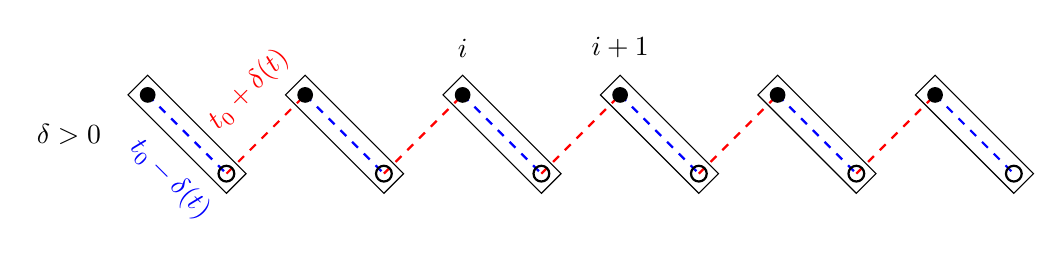
\begin{tikzpicture}
        \draw (-0.25,0) -- (1,-1.25) -- (1.25,-1) -- (0,0.25) -- cycle;
        \draw (1.75,0) -- (3,-1.25) -- (3.25,-1) -- (2,0.25) -- cycle;
        \draw (3.75,0) -- (5,-1.25) -- (5.25,-1) -- (4,0.25) -- cycle;
        \draw (5.75,0) -- (7,-1.25) -- (7.25,-1) -- (6,0.25) -- cycle;
        \draw (7.75,0) -- (9,-1.25) -- (9.25,-1) -- (8,0.25) -- cycle;
        \draw (9.75,0) -- (11,-1.25) -- (11.25,-1) -- (10,0.25) -- cycle;
        \draw[dashed,thick,blue] (0,0) --node[below=1em,rotate=-45]{$t_0-\delta(t)$} (1,-1);
        \draw[dashed,thick,blue] (2,0) -- (3,-1);
        \draw[dashed,thick,blue] (4,0) -- (5,-1);
        \draw[dashed,thick,blue] (6,0) -- (7,-1);
        \draw[dashed,thick,blue] (8,0) -- (9,-1);
        \draw[dashed,thick,blue] (10,0) -- (11,-1);
        \draw[dashed,thick,red] (1,-1) --node[above=1em,rotate=45]{$t_0+\delta(t)$} (2,0);
        \draw[dashed,thick,red] (3,-1) -- (4,0);
        \draw[dashed,thick,red] (5,-1) -- (6,0);
        \draw[dashed,thick,red] (7,-1) -- (8,0);
        \draw[dashed,thick,red] (9,-1) -- (10,0);
        \fill (0,0) circle (0.1);
        \fill (2,0) circle (0.1);
        \fill (4,0)node[above=1em]{$i$} circle (0.1);
        \fill (6,0)node[above=1em]{$i+1$} circle (0.1);
        \fill (8,0) circle (0.1);
        \fill (10,0) circle (0.1);
        \draw[thick] (1,-1) circle (0.1);
        \draw[thick] (3,-1) circle (0.1);
        \draw[thick] (5,-1) circle (0.1);
        \draw[thick] (7,-1) circle (0.1);
        \draw[thick] (9,-1) circle (0.1);
        \draw[thick] (11,-1) circle (0.1);
        \node at (-1,-0.5) {$\delta>0$};
    \end{tikzpicture}
\end{center}
负能态的Berry相位为
\begin{equation}
    \begin{split}
        \gamma&=\int_{BZ}\md k\langle\varphi|i\partial_k|\varphi\rangle\\
        &=\int_{BZ}\md k\frac{1}{2}\left[\sgn(d_x)\sqrt{1-\frac{d_z}{\sqrt{d_x^2+d_z^2}}}i\partial_k\left(\sgn(d_x)\sqrt{1-\frac{d_z}{\sqrt{d_x^2+d_z^2}}}\right)+\sqrt{1+\frac{d_z}{\sqrt{d_x^2+d_z^2}}}i\partial_k\sqrt{1+\frac{d_z}{\sqrt{d_x^2+d_z^2}}}\right]
    \end{split}
\end{equation}
构造三角函数:
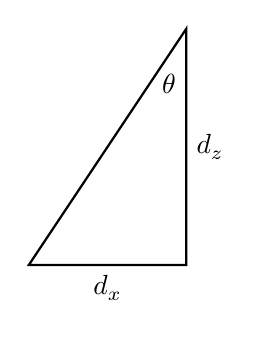
\begin{tikzpicture}
    \draw[thick] (0,0) --node[below]{$d_x$} (2,0) --node[right]{$d_z$} (2,3)node[below=2em,left=0em]{$\theta$} -- cycle;
\end{tikzpicture}
其中满足关系式$\frac{d_z}{\sqrt{d_x^2+d_z^2}}=\cos\theta$
\begin{equation}
    \begin{split}
        Term1&=\sgn(d_x)\sqrt{1-\cos\theta}\partial_k(\sgn(d_x)\sqrt{1-\cos\theta})\\
        &=\sgn(d_x)\sqrt{2\sin^2\frac{\theta}{2}}\left[\partial_k(\sgn(d_x))\sqrt{2\sin^2\frac{\theta}{2}}+\sgn(d_x)\partial_k\sqrt{2\sin^2\frac{\theta}{2}}\right]\\
        &=(\sgn(d_x)\partial_k\sgn(d_x))2\sin^2\frac{\theta}{2}+\partial_k\sin^2\frac{\theta}{2}
    \end{split}
\end{equation}
\begin{equation}
    \begin{split}
        Term2&=\sqrt{1+\cos\theta}\partial_k\sqrt{1+\cos\theta}\\
        &=\sqrt{2\cos^2\frac{\theta}{2}}\partial_k\sqrt{2\cos^2\frac{\theta}{2}}\\
        &=\partial_k\cos^2\frac{\theta}{2}
    \end{split}
\end{equation}
\begin{equation}
    \gamma=\int_{BZ}\md k\frac{i}{2}(Term1+Term2)=\frac{i}{2}\int_{BZ}\md k\partial_k\ln\sgn(d_x)\left(1-\frac{d_z}{\sqrt{d_x^2+d_z^2}}\right)
\end{equation}
\begin{equation}
    d_x=-(t-\delta t)\sin ka,\quad d_z=2\delta t+2(t-\delta t)\sin^2\frac{ka}{2}
\end{equation}
在第一布里渊区内,当$0<k<\frac{\pi}{2}$或者$-\frac{\partial}{2}<k<0$时,$\sgn(d_x)$是一个常数值,对常数值得偏导为$0$。所以积分仅仅在$0$和$\pi$点附近的邻域内有值。
\begin{equation}
    \begin{split}
        \gamma&=\frac{1}{2}\int_{-\frac{\partial}{a}}^{\frac{\partial}{a}}\md k[i\partial_k\ln\sgn(d_x)(1-\frac{d_z}{\sqrt{d_x^2+d_z^2}})]\\
        &=\frac{1}{2}\int_{-\delta}^{\delta}\md k[i\partial_k\ln\sgn(d_x)(1-\sgn(\delta t))]+\frac{1}{2}\int_{\pi-\delta}^{\pi+\delta}\md k[i\partial_k\ln\sgn(d_x)(1-\sgn(t))]\\
        &=\frac{i}{2}[\ln(-1)-\ln1](1-\sgn(\delta t))+\frac{i}{2}p[\ln1-\ln(-1)](1-\sgn(t))\\
        &=\frac{\pi}{2}(\sgn(t)-\sgn(\delta t))\quad \mod{2\pi}
    \end{split}
\end{equation}
对于$\delta t>0$时,$\gamma=0$, 但是对于$\delta t<0$时,$\gamma=\pi$. 这与Dirac模型的结论是一致的。另外的,$Z_2$winding指标为
\begin{equation}
    (-1)^\nu=\delta|_{ka=0}\delta|_{ka=\pi}=\sgn(\frac{t}{\delta t})
\end{equation}
\begin{equation}
    \delta|_{ka=0}=\langle\varphi|P|\varphi\rangle=\frac{1}{2}\begin{pmatrix}
        \sgn(d_x)\sqrt{1-\sgn(\delta t)}&\sqrt{1+\sgn(\delta t)}
    \end{pmatrix}P\begin{pmatrix}
        \sgn(d_x)\sqrt{1-\sgn(\delta t)}\\
        \sqrt{1+\sgn(\delta t)}
    \end{pmatrix}=\sgn(\delta t)
\end{equation}
\begin{equation}
    \delta|_{ka=\pi}=\langle\varphi|P|\varphi\rangle=\frac{1}{2}\begin{pmatrix}
        \sgn(d_x)\sqrt{1-\sgn(t)}&\sqrt{1-\sgn(t)}
    \end{pmatrix}P\begin{pmatrix}
        \sgn(d_x)\sqrt{1-\sgn(t)}\\
        \sqrt{1+\sgn(t)}
    \end{pmatrix}=\sgn(t)
\end{equation}
Berry相位或者Winding数的改变伴随着$\delta t=0$附近能隙的关闭和重新打开。这可以被看成能隙从正变化到负。$\delta t=0$时,能隙为$0$,能级在$k=0$处交叠。在这一点附近做线性展开得到
\begin{equation}
    H=\sum_{k}\psi_k^\dagger[-(t-\delta t)ka\sigma_x+(2\delta t+\frac{1}{2}(t-\delta t)k^2a^2)\sigma_z]\psi
\end{equation}
这正是狄拉克方程的连续模型。这样,我们可以定义能隙$\Delta E=4\delta t$, 不是$4|\delta t|$. $\delta t$的符号改变表明了拓扑相变。
\begin{figure}[h]
    \centering
    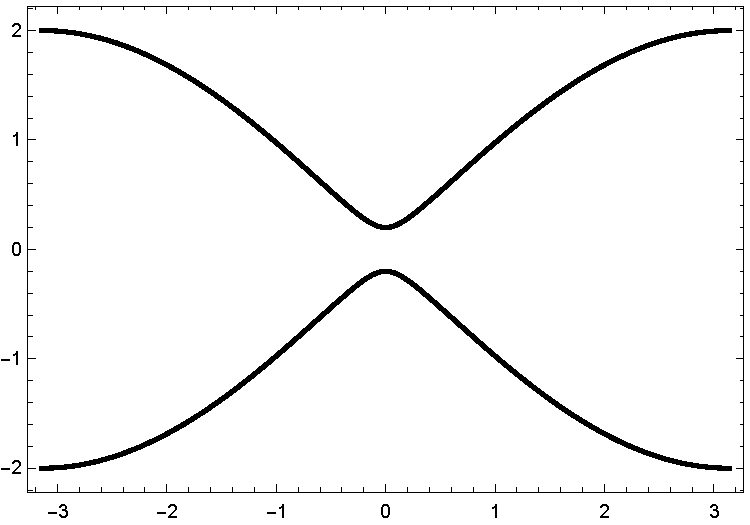
\includegraphics[width=2in]{SSHenergy1.pdf}
    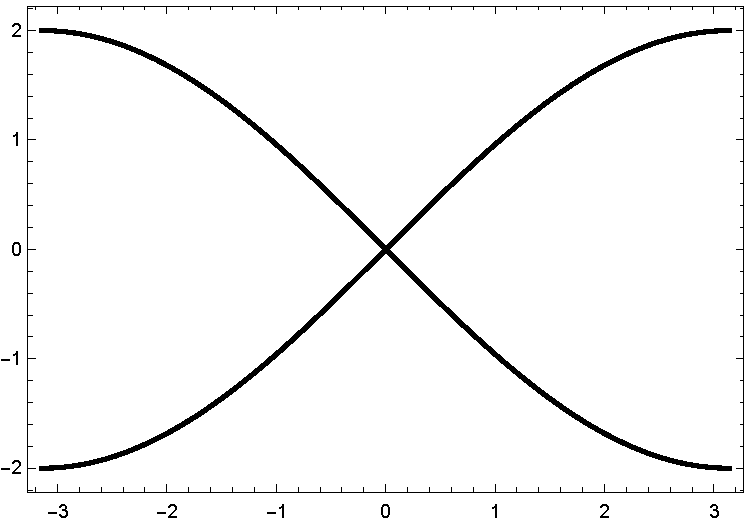
\includegraphics[width=2in]{SSHenergy2.pdf}
    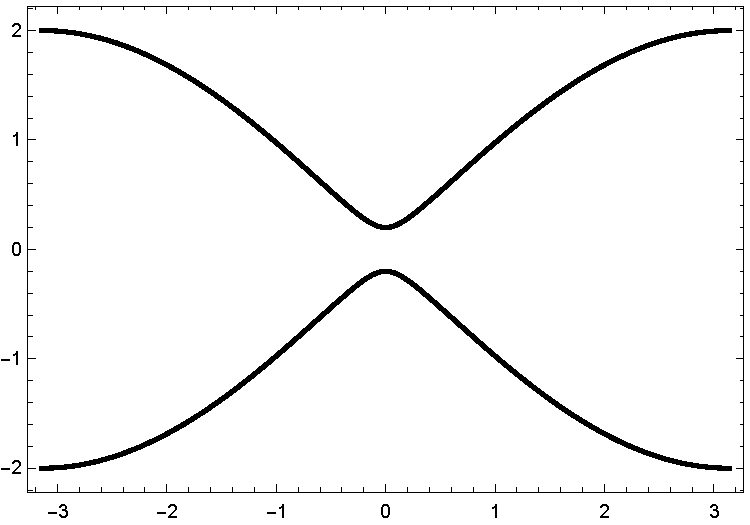
\includegraphics[width=2in]{SSHenergy3.pdf}
    \caption{\footnotesize{SSH模型能量色散关系,$\delta>0$,$\delta=0$,$\delta<0$. 能隙在$\delta=0$附近关闭再打开表明发生了量子相变。}}\label{dirac pic 7}
\end{figure}
当Berry相位为$\pi$或者Winding指数为$\nu=1$时,开边界条件末端态的存在是拓扑相的特征。应该注意,开边界条件意味着链在两个原胞之间剪断,而不是在原胞内的两个格点之间。假设$t>0$,对于$\delta t>0$是拓扑平凡的,对于$\delta t<0$是拓扑非平凡的。换句话说,如果末端键是长键,$|t+\delta t|<|t-\delta t|$,那就是拓扑非平凡的。否则就是拓扑平凡的。

拓扑量子相变发生在$\delta t=0$处。在长波极限下,当$\delta t<0$时,我们可以利用修正狄拉克方程束缚态解。在这种情况,在末端附近存在零模解。波函数空间分布主要有特征长度决定
\begin{equation}
    \xi_-=\frac{2|B|\hbar}{v}(1-\sqrt{1-4mB})^{-1}\to\frac{\hbar}{|m|v}=\frac{t-\delta t}{2|\delta t|}
\end{equation}
当$\delta t\to0$时,特征长度发散,这意味着末端态演化成体态,并且系统变成无能隙的。当$\delta>0$时,没有末端态。因此这个事实解释了$\delta t=0$附近的拓扑量子相变。

我们可以用数值计算理论来计算能量本征态,通过对角化得到能量本征值
\begin{equation}
    \begin{pmatrix}
        0&t+\delta t&\\
        t+\delta t&0&t-\delta t\\
        \quad&t-\delta t&0&t+\delta t\\
        \quad&\quad&t+\delta t&0&t-\delta t\\
        \quad&\quad&\quad&t-\delta t&0&\ddots&\\
        \quad&\quad&\quad&\quad&\ddots&0&t+\delta t\\
        \quad&\quad&\quad&\quad&\quad&t+\delta t&0
    \end{pmatrix}
\end{equation}
当改变$\delta t$符号时,可以找到末端处的零模存在。末端态在$\delta t=-0.1 t$和$\delta t=-0.3t$如图。这解释了对于很小的$|\delta t|$波函数有一个更宽的空间分布。
\begin{figure}[h]
    \centering
    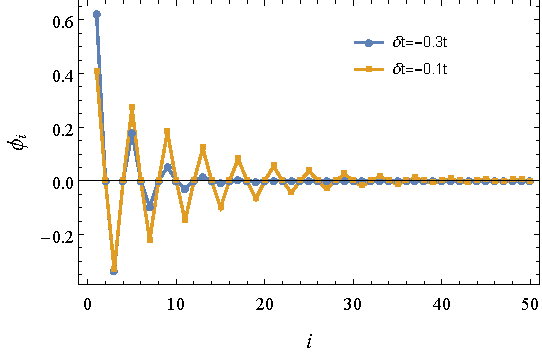
\includegraphics[width=6in]{SSHFunc.pdf}
    \caption{\footnotesize{在格点$i$上的末端态波函数$\Psi_i$的振幅,其中$\delta t=-0.1$和$\delta t=-0.3$. $\delta t$越小意味着波函数在空间的分布越宽。}}
\end{figure}

然而这个模型最著名的激发是孤子激发和反孤子激发,这是聚乙炔中的电荷和自旋的载流子。他们是$\pi$相和$0$相这俩截然不同相的domain wall. 这些解对应于在正负质量区域界面上的狄拉克方程。带隙束缚态的波函数分布在domain wall的周围。考虑电子自旋简并,不同自旋有两个束缚态。孤子的电荷态和自旋态随局域化化学键表示的domain wall的解而变化。根据这两种状态的电子数$n$,总共有四种可能的状态:(a)对于$n=1$,两个中性自旋$\frac{1}{2}$,$S_z=\pm\frac{1}{2}$的孤子; (b)当$n=0$和$n=2$时,两类电荷$S^{\pm}$,其中总自旋为零,可视为无自旋的“离子”。然而,与化学类似物相反,孤子可以自由移动,除非它们被固定住。从拓扑绝缘子的观点来看,这些状态是拓扑平凡相位和拓扑非平凡相位之间的界面末端状态。

\subsection{非厄米SSH}

\subsection{拓扑铁磁物质}
在SSH模型中,哈密顿被写成以$A,B$两个子格为基$(a_k^\dagger,b_k^\dagger)$的$2\times 2$矩阵。如果我们把$A,B$两个子格换成两个不同自旋的电子$(c_{k\uparrow}^\dagger,c_{k\downarrow}^\dagger)$可以得到一类新的一维拓扑相。对于自旋轨道耦合铁磁,哈密顿写成
\begin{equation}
    H=\sum_{k}(c_{k\uparrow}^\dagger,c_{k\downarrow}^\dagger)\left[\lambda\sin k+(M-4B\sin^2\frac{k}{2})\sigma_z\right]\begin{pmatrix}
        c_{k\uparrow}\\
        c_{k\downarrow}
    \end{pmatrix}
\end{equation}
其中$c_{k,\sigma}^\dagger$和$c_{k,\sigma}$是电子自旋$\sigma=(\uparrow,\downarrow)$的产生湮灭算符。这里$\lambda$是强自旋轨道耦合。在没有自旋轨道耦合的情况下,自旋向上和向下的两个电子带可以很好地分离。如果较低能带被完全填满,则基态被最大自旋完全饱和,并且系统是一个绝缘铁磁体。在自旋轨道耦合出现的情况下,总自旋$S_z$不再是守恒量。但是,由于$Sz$的期望值仍然是非零,满带仍然是铁磁性的。我们发现,该模型与SSH模型具有相同的数学结构,尽管两种模型的基础不同。它描述了一维拓扑铁磁体。

\section{1-D/2-D拓扑超流}
\subsection{p波超导}
$p$波无自旋配对超导体有两个明显的相,强配对和弱配对相,分别对应拓扑平凡和拓扑非平凡相。在BCS理论里,超导体的有效模型为
\begin{equation}
    H=\sum_{k}(\frac{\hbar^2 k^2}{2m}-\mu)c_k^\dagger c_k+\Delta_k^* c_{-k}c_{k}+\Delta_k c_{k}^\dagger c_{-k}^\dagger
\end{equation}
其中$\mu$是化学势,决定了电子数。引入旋量$(c_k^\dagger,c_{-k})$可以得到
\begin{equation}
    \begin{split}
        H&=\sum_{k}(c_k^\dagger,c_{-k})\begin{pmatrix}
            \frac{1}{2}(\frac{\hbar^2 k^2}{2m}-\mu)&\Delta_k\\
            \Delta_k^*&-\frac{1}{2}(\frac{\hbar^2k^2}{2m}-\mu)
        \end{pmatrix}\begin{pmatrix}
            c_k\\
            c_{-k}^\dagger
        \end{pmatrix}\\
        &=\sum_{k}(c_k^\dagger,c_{-k})\begin{pmatrix}
            \frac{1}{2}(\frac{\hbar^2 k^2}{2m}-\mu)&\Delta_k\\
            \Delta_k&-\frac{1}{2}(\frac{\hbar^2k^2}{2m}-\mu)
        \end{pmatrix}\begin{pmatrix}
            c_k\\
            c_{-k}^\dagger
        \end{pmatrix}
    \end{split}
\end{equation}
改写成BdG形式时多的常数$\frac{1}{2}\sum_{k}(\frac{\hbar^2 k^2}{2m}-\mu)$被忽略掉了。等式第二行通过$U(1)$规范选择可以把序参数变成实数。对于$p$波配对超导,Cooper对的序参数满足$\Delta_k=-\Delta_{-k}$. 为了简单起见,我们令$\Delta_k=\Delta_0 k$. 上述哈密顿可以写成一维连续系统狄拉克哈密顿
\begin{equation}
    H(k)=\Delta_k\sigma_x+\frac{1}{2}(\frac{\hbar^2 k^2}{2m}-\mu)\sigma_z=\mathbf{d}\cdot\msigma
\end{equation}
其中$d_x=\Delta_k$, $d_z=\frac{1}{2}(\frac{\hbar^2 k^2}{2m}-\mu)$. 带入上节的Berry相位表达式里得到
\begin{equation}
    \begin{split}
        \gamma&=\oint\md k\langle\varphi|i\partial_k|\varphi\rangle\\
        &=\frac{1}{2}\int_{-\infty}^{+\infty}\md k(i\partial_k\ln\sgn(d_x))(1-\frac{d_z}{\sqrt{d_x^2+d_z^2}})\\
        &=\frac{1}{2}\int_{-\infty}^{+\infty}\md k(i\partial_k\ln\sgn(\Delta_0 k))(1-\frac{\frac{1}{2}(\frac{\hbar^2 k^2}{2m}-\mu)}{\sqrt{\Delta_0k^2+\frac{1}{4}(\frac{\hbar^2 k^2}{2m}-\mu)^2}})\\
        &=\frac{i}{2}[\ln1-\ln(-1)](1-\sgn(-\mu))
    \end{split}
\end{equation}
对于化学势$\mu>0$,基态的Berry相位总是$\pi$,这里我们假设质量$m$是正的。在这个系统里,如果$\Delta=0$\
\begin{equation}
    \begin{split}
        H&=\frac{1}{2}\sum_{k}\begin{pmatrix}
            c_k^\dagger&c_{-k}
            \end{pmatrix}(\frac{\hbar^2k^2}{2m}-\mu)\sigma_z\begin{pmatrix}
                c_k\\
                c_{-k}^\dagger
        \end{pmatrix}\\
        &=\sum_{k}(\frac{\hbar^2 k^2}{2m}-\mu)c_k^\dagger c_k-\frac{1}{2}\sum_{k}(\frac{\hbar^2 k^2}{2m}-\mu)
    \end{split}
\end{equation}
本征值为$\pm\frac{1}{2}(\frac{\hbar^2 k^2}{2m}-\mu)$的两个态实际上对应的是一个态。这是由于旋量基的冗余。这就是所谓的粒子空穴对称性,即使在$\Delta\neq0$的情况下也成立。
稍微求一下$p$波超导下的$\mathcal{C}$算符表示矩阵
\begin{equation}
    Particle\;Hole\;\mathcal{C}:c_{p\sigma}\longrightarrow c_{-p\sigma}^\dagger
\end{equation}
\begin{equation}
    \mathcal{C}\begin{pmatrix}
        c_{k}\\
        c_{-k}^\dagger
    \end{pmatrix}\mathcal{C}=\begin{pmatrix}
        c_{-k}^\dagger\\
        c_k
    \end{pmatrix}=\sigma_x\begin{pmatrix}
        c_{k}\\
        c_{-k}^\dagger
    \end{pmatrix}
\end{equation}
在这个基下Particle-Hole变换的表示矩阵:$D(\mathcal{C})=\sigma_x$
\begin{equation}
    \begin{split}
        -D(\mathcal{C})H_{BdG}^T(-k)D(\mathcal{C})&=\sigma_x(-\Delta_{-k}\sigma_x^T-\frac{1}{2}(\frac{\hbar^2 k^2}{2m}-\mu)\sigma_z^T)\sigma_x\\
        &=-\Delta_{-k}\sigma_x+\frac{1}{2}(\frac{\hbar^2 k^2}{2m}-\mu)\sigma_z\\
        &=\Delta_k\sigma_x+\frac{1}{2}(\frac{\hbar^2 k^2}{2m}-\mu)\sigma_z=H_{BdG}(k)
    \end{split}
\end{equation}
p波超导满足Particle-Hole对称性。

在晶格上,$k$和$k^2$可以替换成$\sin k$和$4\sin^2\frac{k}{2}$. 有效模型为
\begin{equation}
    H=\sum_{k}\begin{pmatrix}
        c_k^\dagger&c_{-k}
    \end{pmatrix}\left[\Delta_0\sin k\sigma_x+(t+4t'\sin^2\frac{k}{2})\sigma_z\right]\begin{pmatrix}
        c_k\\
        c_{-k}^\dagger
    \end{pmatrix}
\end{equation}
准粒子谱能量本征值为
\begin{equation}
    E_{\pm,k}=\pm\sqrt{\Delta_0^2\sin^2 k+(t+4t'\sin^2\frac{k}{2}^2)}
\end{equation}
这里,$t=-\frac{\mu}{2},t'=\frac{\hbar^2}{4m}$. 我们把k空间哈密顿傅里叶变换到实空间里得到
\begin{equation}
    \begin{split}
        H&=\sum_{k}\Delta_0\frac{e^{ik}-e^{-ik}}{2i}\frac{1}{N}\sum_{i,j}e^{ik(r_i-r_j)}c_i^\dagger c_j^\dagger+h.c.+\sum_{k}2(t+4t'\sin^2\frac{k}{2})\frac{1}{N}\sum_{i,j}e^{ik(r_i-r_j)}c_i^\dagger c_j\\
        &=\frac{1}{N}\sum_{k,i,j}\frac{\Delta_0}{2i}[e^{ik(r_i-r_j+1)}-e^{ik(r_i-r_j-1)}]c_i^\dagger c_j^\dagger+h.c.+\frac{1}{N}\sum_{k,i,j}2(t+4t'\frac{1-\cos k}{2})e^{ik(r_ir_j)}c_i^\dagger c_j\\
        &=2(t+2t')\sum_{i}c_i^\dagger c_i-2t'\sum_{i}c_i^\dagger c_{i+1}+h.c.-i\Delta_0\sum_{i}c_ic_{i+1}+h.c.
    \end{split}
\end{equation}
这就是一维马约拉纳费米子的Kitaev模型。

当系统有一个开边界条件时,对于拓扑非平凡相,在边界附近存在一个零能模,满足
\begin{equation}
    \gamma^\dagger(E=0)=\gamma(E=0)
\end{equation}
这样,零模的产生算符等于它自身的湮灭算符。这样的粒子被叫做马约拉纳费米子。由于Particle-Hole对称性,这样的两个态实际上在Particle-Hole变换后对应的是一个态。因此,基态是双重简并的,这取决于零能量模是否被占据。由于有效哈密顿量中的库珀配对项成对地产生或湮灭电子,电子的宇称数总是守恒的。由于有效哈密顿量中的库珀配对项成对地产生或湮灭电子,电子的宇称数总是守恒的。零模的占据会改变系统的奇偶宇称数。

p波配对超导和SSH模型通过部分Particle-Hole变换联系起来。对格点B上的电子做一个Particle-Hole变换得到
\begin{equation}
    c_{B,n}\rightarrow c_{B,n}^\dagger
\end{equation}
SSH模型变成
\begin{equation}
    H=\sum_{n=1}^N(t+\delta t)c_{A,n}^\dagger c_{B,n}^\dagger+\sum_{n=1}^{N-1}(t-\delta t)c_{A,n+1}\dagger c_{B,n}^\dagger+h.c.
\end{equation}
这是一个在晶格上的p波配对超导。


\subsection{一维p波超导}
拓扑超导的最简单粒子就是一维二维无自旋费米子的BdG平均场哈密顿。无自旋费米子也可以被看为更加复杂有自旋的情况或者简单看为源于TR对称性破缺的完全自旋极化费米子的玩具模型。我们将首先考虑具有p波超导性的一维链,然后再讨论二维手性p波超导体,两者都表现出拓扑超导相。
\subsubsection{1-D p波超导}
\subsubsection{2-D p+ip波超导}
\subsection{一般超流配对}
设$c_{k\alpha}^\dagger$是自旋$1/2$费米子的产生湮灭算符,波矢为$\mk$,自旋投影$\alpha=\uparrow,\downarrow$. 质心动量为$0$的一般配对态的配对振幅。定义为
\begin{equation}
    \psi_{\alpha,\beta}=\langle c_{k,\alpha}c_{-k,\beta}\rangle
\end{equation}
首先,我们研究在自旋空间里转动下的配对振幅一般性质。自旋空间$SU(2)$转动矩阵绕$\mathbf{n}$无穷小转动形式为
\begin{equation}\label{rotation R}
    R=1+\frac{i}{2}\mn\cdot\sigma\delta \theta
\end{equation}
其中$\sigma=(\sigma_x,\sigma_y,\sigma_z)$是泡利矩阵的矢量形式。
\begin{equation}
    \sigma_x=\begin{pmatrix}
        0&1\\
        1&0
    \end{pmatrix},\quad\sigma_y=\begin{pmatrix}
        0&-i\\
        i&0
    \end{pmatrix},\quad\sigma_z=\begin{pmatrix}
        1&0\\
        0&-1
    \end{pmatrix}
\end{equation}
在这个转动\eqref{rotation R}下,配对振幅$\psi_{\alpha,\beta}$变化形式为
\begin{equation}
    \psi_{\alpha,\beta}'=R_{\alpha\gamma}R_{\beta\delta}\psi_{\gamma\delta}=R_{\alpha\gamma}\psi_{\gamma\delta}(R_{\delta\beta})^T
\end{equation}
其中$T$表示转置。因为$\sigma^T=-\sigma_y\sigma\sigma_y$,我们得到
\begin{equation}
    \begin{split}
        \psi_{\alpha\beta}&=\left(1+\frac{i}{2}\mn\cdot\sigma\delta\theta\right)_{\alpha\gamma}\psi_{\gamma\delta}\left(1-\frac{i}{2}\mn\cdot\sigma_y\sigma\sigma_y\delta\theta\right)_{\delta\beta}\\
        &=\left[\psi+\frac{i}{2}(\mn\cdot\sigma)_{\alpha\gamma}\delta\theta\psi_{\gamma\delta}-\frac{i}{2}\psi_{\gamma\delta}(\mn\cdot\sigma_{y}\sigma\sigma_y)_{\delta\beta}\delta\theta\right]\\
        &=\left[\psi+\frac{i}{2}\mn\cdot(\sigma\psi)_{\alpha\delta}\delta\theta-\frac{i}{2}\mn\cdot(\psi\sigma_y\sigma\sigma_y)_{\gamma\beta}\delta\theta\right]\\
        &=\left[\psi+\frac{i}{2}\mn\cdot(\sigma\psi\sigma_y-\psi\sigma_y\sigma)\sigma_y\delta\theta\right]_{\alpha\beta}
    \end{split}
\end{equation}
这里我们忽略掉了$\delta\theta^2$项,并且定义$2\times2$矩阵$\psi=(\psi_{\alpha\beta})$. 写成矢量形式
\begin{equation}
    \mpsi'=\mpsi+\frac{i}{2}\mn\cdot(\msigma\mpsi\sigma_y-\psi\sigma_y\msigma)\sigma_y\delta\theta
\end{equation}
任意$2\times 2$矩阵都可以表示成$A_0\sigma_0+\mathbf{A}\cdot\msigma$. 在自旋空间的$SU(2)$的一个转动,自旋singlet$\mpsi^{singlet}$和自旋triplet$\mpsi^{triplet}$分别按照标量和矢量变化。
\begin{equation}
    \mpsi^{singlet}=A_0(\mk)i\sigma_y
\end{equation}
\begin{equation}
    \mpsi^{triplet}=\mathbf{A}(\mk)\cdot i\msigma\sigma_y
\end{equation}
其中$\mathbf{A}=(A_x,A_y,A_z)$. 事实上,把上面第一式带入$SU(2)$无穷小变换里,可以看到$\mpsi'=\mpsi$. 此外第二式带入无穷小变换得到
\begin{equation}
    \begin{split}
        \mpsi'^{triplet}&=\mpsi^{triplet}+\frac{i}{2}\mn\cdot(\msigma\mpsi^{triplet}\sigma_y-\mpsi^{triplet}\sigma_y\msigma)\sigma_y\delta\theta\\
        &=\mpsi^{triplet}+\frac{i}{2}[(\mn\cdot\msigma)(iA\cdot\msigma)-(iA\cdot\msigma)(\mn\cdot\msigma)]\\
        &=\mpsi^{triplet}-\frac{1}{2}[(\mn\cdot\sigma)(A\cdot\msigma)-(A\cdot\msigma)(\mn\cdot\msigma)]\\
        &=\mpsi^{triplet}-\frac{1}{2}[\sigma_n,A\cdot\msigma]
    \end{split}
\end{equation}
稍微计算一下
\begin{equation}
    \begin{split}
        (\mn\cdot\msigma)(\mathbf{A}\cdot\msigma)=n_i\sigma_iA_j\sigma_j=n_iA_j(\delta_{ij}+i\epsilon_{ijk}\sigma_k)\Rightarrow(\mn\cdot\msigma)(\mathbf{A}\cdot\msigma)-(\mathbf{A}\cdot\msigma)(\mn\cdot\msigma)=2i(\mn\times\mathbf{A})\cdot\msigma
    \end{split}
\end{equation}
得到
\begin{equation}
    \mpsi'^{triplet}=\mpsi^{triplet}-i(\mn\times A)\cdot\msigma\sigma_y\delta\theta
\end{equation}
这样,我们可以看到Triplet$\psi^{triplet}$的确是向量。

由于$c_{\mk\alpha}$的反对易关系,在交换两个粒子的请况下,$\psi_{\alpha\beta}(k)$必须改变符号。
\begin{equation}
    \psi_{\beta\alpha}(-k)=\langle c_{-k\beta}c_{k\alpha}\rangle=-\langle c_{k\alpha}c_{-k\beta}\rangle=-\psi_{\alpha\beta}(k)
\end{equation}
这说明轨道部分必须满足
\begin{equation}
    A_0(-\mk)=A_0(-\mk)
\end{equation}
\begin{equation}
    \mathbf{A}(-\mk)=-\mathbf{A}(\mk)
\end{equation}
这是由于$i\sigma_y=\begin{pmatrix}
    0&1\\
    -1&0
\end{pmatrix}$, 自旋单态配对振幅$\psi^{singlet}=A_0(\mk)i\sigma_y$,对于自旋triplet $\psi^{triplet}=\mathbf{A}(\mk)\cdot i\msigma\sigma_y$. 自旋部分矩阵为$i\msigma\sigma_y=(i\sigma_x\sigma_y,i\sigma_y^2,i\sigma_z\sigma_y)=(-\sigma_z,i,\sigma_x)$都是对称矩阵。我们可以看到最一般的配对振幅可以写成
\begin{equation}
    \mpsi=A_0\begin{pmatrix}
        0&1\\
        -1&0
    \end{pmatrix}+A_x\begin{pmatrix}
        -1&0\\
        0&1
    \end{pmatrix}+A_y\begin{pmatrix}
        i&0\\
        0&i
    \end{pmatrix}+A_z\begin{pmatrix}
        0&1\\
        1&0
    \end{pmatrix}=\begin{pmatrix}
        -A_x+iA_y&A_0+A_z\\
        -A_0+A_z&A_x+iA_y
    \end{pmatrix}
\end{equation}
超流能隙函数为
\begin{equation}\label{gap func}
    \Delta_{\alpha\beta}(\mk)=\sum_{k'\alpha',\beta'}V_{\alpha\beta\alpha'\beta'}(\mk,\mk')\psi_{\alpha'\beta'}(\mk')
\end{equation}
其中$V_{\alpha\beta\alpha'\beta'}(\mk,\mk')$是费米子之间相互作用哈密顿的矩阵元
\begin{equation}
    V=\frac{1}{2\Omega}\sum_{\mk,\mk',\mathbf{q},\alpha,\beta,\alpha'\beta'}V_{\alpha\beta\alpha'\beta'}(\mk,\mk')c_{-\mk+\frac{\mathbf{q}}{2},\beta}^\dagger c_{\mk+\frac{\mathbf{q}}{2}\alpha}^\dagger c_{\mk'+\frac{\mathbf{q}}{2},\alpha'}c_{-\mk'+\frac{q}{2},\beta'}
\end{equation}
矩阵元满足
\begin{equation}
    V_{\beta\alpha\alpha'\beta'}(-\mk,\mk')=V_{\alpha\beta\beta'\alpha'}(\mk,-\mk')=-V_{\alpha\beta\alpha'\beta'}(\mk,\mk')
\end{equation}
由于$V$的厄米性我们有
\begin{equation}
    V_{\alpha'\beta'\alpha\beta}(\mk',\mk)=V_{\alpha\beta\alpha'\beta'}^*(\mk,\mk')
\end{equation}
当相互作用当相互作用保证自旋角动量守恒时,矩阵元有如下形式
\begin{equation}\label{int equation}
    V_{\alpha\beta\alpha'\beta'}(\mk,\mk')=\frac{1}{2}(\delta_{\alpha\alpha'}\delta_{\beta\beta'}-\delta_{\alpha\beta'}\delta_{\alpha'\beta})V^{(e)}(\mk,\mk')+\frac{1}{2}(\delta_{\alpha\alpha'}\delta_{\beta\beta'}+\delta_{\alpha\beta'}\delta_{\alpha'\beta})V^{(o)}(\mk,\mk')
\end{equation}
$V^{(e)}$和$V^{(o)}$分别描述偶宇称和奇宇称部分:
\begin{equation}
    V^{(e)}(-\mk,\mk')=V^{(e)}(\mk,-\mk')=V^{(e)}(\mk,\mk')
\end{equation}
\begin{equation}
    V^{(o)}(-\mk,\mk')=V^{(o)}(\mk,-\mk')=-V^{(o)}(\mk,\mk')
\end{equation}
方程\eqref{int equation}带入能隙方程\eqref{gap func}中得到
\begin{equation}
    \Delta_{\alpha\beta}(\mk)=\frac{1}{2}\sum_{\mk'}\left\{[\psi_{\alpha\beta}(\mk')-\psi_{\beta\alpha}(\mk')]V^{(e)}(\mk,\mk')+[\psi_{\alpha\beta}(\mk')+\psi_{\beta\alpha}(\mk')]V^{(o)}(\mk,\mk')\right\}
\end{equation}
右手边第一项描述自旋单态配对
\begin{equation}
    \Delta^{singlet}(\mk)=\frac{1}{2}\sum_{\mk'}\begin{pmatrix}
        0&\psi_{\uparrow\downarrow}(\mk')-\psi_{\downarrow\uparrow}(\mk')\\
        -(\psi_{\uparrow\downarrow}(\mk')-\psi_{\downarrow\uparrow}(\mk'))&0
    \end{pmatrix}V^{(e)}(\mk,\mk')=\sum_{\mk'}\frac{1}{2}(\psi_{\uparrow\downarrow}(\mk')-\psi_{\downarrow\uparrow}(\mk'))V^{(e)}(\mk,\mk')i\sigma_y
\end{equation}
定义
\begin{equation}
    \begin{split}
        \Delta(\mk)&=\sum_{\mk}A_{0}(\mk)V^{(e)}(\mk,\mk')\\
        A_0(\mk)&=\frac{1}{2}(\psi_{\uparrow\downarrow}(\mk')-\psi_{\downarrow\uparrow}(\mk'))
    \end{split}
\end{equation}
第二项描述自旋三重态配对
\begin{equation}
    \Delta^{triplet}(\mk)=\frac{1}{2}\sum_{\mk'}\begin{pmatrix}
        2\psi_{\uparrow\uparrow}(\mk')&\psi_{\uparrow\downarrow}(\mk')+\psi_{\downarrow\uparrow}(\mk')\\
        \psi_{\uparrow\downarrow}(\mk')+\psi_{\downarrow\uparrow}(\mk')&2\psi_{\downarrow\downarrow}(\mk')
    \end{pmatrix}V^{(o)}(\mk,\mk')
\end{equation}
\begin{equation}
    \mathbf{A}(\mk)\cdot i\msigma\sigma_y=\begin{pmatrix}
        -A_x+iA_y&A_z\\
        A_z&A_x+iA_y
    \end{pmatrix}
\end{equation}
比较得知
\begin{equation}
    \begin{cases}
        -A_x+iA_y=\psi_{\uparrow\uparrow}(\mk)\\
        A_x+iA_y=\psi_{\downarrow\downarrow}(\mk)\\
        A_z=\frac{1}{2}(\psi_{\uparrow\downarrow}(\mk)+\psi_{\downarrow\uparrow}(\mk'))
    \end{cases}\Longrightarrow\begin{cases}
        A_x=-\frac{\psi_{\uparrow\uparrow}(\mk)-\psi_{\downarrow\downarrow}(\mk)}{2}\\
        A_y=\frac{\psi_{\uparrow\uparrow}(\mk)+\psi_{\downarrow\downarrow}(\mk)}{2i}\\
        A_z=\frac{\psi_{\uparrow\downarrow}(\mk)+\psi_{\downarrow\uparrow}(\mk)}{2}
    \end{cases}
\end{equation}
\begin{equation}
    \Delta^{triplet}(\mk)=\sum_{\mk'}\mathbf{A}(\mk')\cdot i\msigma\sigma_y V^{(o)}(\mk,\mk')
\end{equation}
定义
\begin{equation}
    \mDelta(\mk)=\sum_{\mk'}\mathbf{A}(\mk')V^{(o)}(\mk,\mk')
\end{equation}
所以有
\begin{equation}\label{triplet gap}
    \Delta^{triplet}(\mk)=\mDelta(\mk)\cdot i\msigma\sigma_y
\end{equation}
因为$\mathbf{A}(\mk)$在自旋空间里按照矢量形式变化,所以$\mDelta(\mk)$也是如此。由方程\eqref{triplet gap}可以知
\begin{equation}
    \begin{split}
        \Delta^{triplet}(\Delta^{triplet})^\dagger&=(\mDelta\cdot i\msigma\sigma_y)(-i\sigma_y\msigma\cdot\mDelta^*)=(\mDelta\cdot\msigma)(\msigma\cdot\mDelta^*)\\
        &=\mDelta_i\mDelta_j^*\sigma_i\sigma_j=\mDelta_i\mDelta_j^*(\delta_{ij}+i\epsilon_{ijk}\sigma_k)\\
        &=\mDelta\cdot\mDelta^*+i(\mDelta\times\mDelta^*)\cdot\msigma
    \end{split}
\end{equation}
沿着$\mDelta\times\mDelta^*$的方向建立坐标轴,我们可以看到对于自旋三重态的能隙本征值为
\begin{equation}
    \sqrt{|\mDelta|^2\pm|\mDelta\times\mDelta^*|^2}
\end{equation}
$\mDelta\times\mDelta^*=0$的配对态被称为幺正的,$\mDelta\times\mDelta^*\neq0$的配对态被称为非幺正的。换句话说,如果对于所有的相,矢量$\mDelta$是实的,则配对态就是幺正的,对于幺正态,能隙由$|\mDelta(\mk)|$给出,激发谱为
\begin{equation}
    E_{\mk}=\sqrt{\xi_k^2+|\mDelta(\mk)|^2}
\end{equation}
非幺正态的性质可以通过考虑$\Delta_z=0$的情况来说明
\begin{equation}
    \mDelta\times\mDelta^*=\begin{pmatrix}
        0,0,\Delta_x\Delta_y^*-\Delta_y\Delta_x^*
    \end{pmatrix}
\end{equation}
定义
\begin{equation}
    \Delta_{\uparrow\uparrow}=-\Delta_x+i\Delta_y=\sum_{k'}V^{(0)}(\mk,\mk')[-A_x(\mk')+iA_y(\mk')]=\sum_{k'}V^{(0)}(\mk,\mk')\psi_{\uparrow\uparrow}(\mk')
\end{equation}
\begin{equation}
    \Delta_{\downarrow\downarrow}=\Delta_x+i\Delta_y=\sum_{k'}V^{(0)}(\mk,\mk')[A_x(\mk')+iA_y(\mk')]=\sum_{k'}V^{(0)}(\mk,\mk')\psi_{\downarrow\downarrow}(\mk')
\end{equation}
所以$z$分量为
\begin{equation}
    \Delta_x\Delta_y^*-\Delta_y\Delta_x^*=\frac{|\Delta_{\uparrow\uparrow}|^2-|\Delta_{\downarrow\downarrow}|^2}{2i}
\end{equation}
对于非幺正情况,考虑$\Delta_z=0$
\begin{equation}
    \mDelta\times\mDelta^*=\begin{pmatrix}
        0,0,\frac{|\mDelta_{\uparrow\uparrow}|^2-|\mDelta_{\downarrow\downarrow}|^2}{2i}
    \end{pmatrix}
\end{equation}
因此,能隙依赖于自旋方向。

当相互作用在同时转动$\mk$和$\mk'$下不变时,$V(k,k')$可以球面波展开为
\begin{equation}
    V(k,k')=\sum_{l=0}^{\infty}V_{l}(k,k')P_l(\hat{k}\cdot\hat{k}')
\end{equation}
其中$P_l$是勒让德多项式,$\hat{k}=\frac{\mk}{k}$. $s$波超导能隙方程替换成一般情况的能隙方程
\begin{equation}
    \Delta_{\alpha\beta}(\mk)=-\frac{1}{\Omega}\sum_{\mk'}V_{l}(k,k')\frac{\Delta_{\alpha\beta}(\mk')}{2E_{\mk,\alpha}}(1-2f(E_{k,\alpha}))
\end{equation}
假设$V_l$仅仅在费米面附近非零并且为常数,我们可以把它拿出求和号里,这样得到
\begin{equation}
    1=-D(E_F)V_l\int_0^{\omega_c}d\xi\frac{\tanh\frac{\beta_c\xi}{2}}{\xi}
\end{equation}
这样,相变温度$T_c=\frac{1}{k_B\beta}$由大多数吸引相互作用$V_l$的$l$决定


%\section{拓扑分类}
%继Altland和Zirnbauer之后,可以系统地列举出任意矩阵的所有可能的对称类,这些任意的矩阵可以解释为某些非相互作用费米子系统的哈密顿量:总共有10个对称类。所有的类都是在一些离散对称性下具有特定变换性质哈密顿的集合。

%考虑一个一般无相互作用费米子系统,二次量子化表述为
%\begin{equation}
%    H=\sum_{A,B}\psi_A^\dagger H_{A,B}\psi_B
%\end{equation}
%其中$\psi_A^\dagger$和$\psi_B$是费米子产生湮灭算符,满足
%\begin{equation}
%    \{\psi_A^\dagger,\psi_B\}=\delta_{A,B}
%\end{equation}
%角标$A,B$可以是集体指标。例如对于一个晶格上的电子系统,$A=(i,\sigma)$,这表示在格点$i$上自旋为$\sigma$的电子。在这个情况下$H_{A,B}$是一个方块矩阵。哈密顿的对称性意味着哈密顿$H$与$-H,H^T$以及$H^*$有关。我们要求这些变换由幺正变换实现并且他们的平方作用在哈密顿上为$1$. 因此我们考虑如下变换
%\begin{enumerate}
%    \item P对称:$H=-PHP^{-1}$, 其中$PP^\dagger=P^2=1$
%    \item C对称:$H=\epsilon_C CH^TC^{-1}$, 其中$CC^{\dagger}=1$以及$C^T=\eta_CC$($\epsilon_C=\pm1, \eta_C=\pm1$)
%    \item K对称:$H=\epsilon_K KH^*K^{-1}$, 其中$KK^\dagger=1$以及$K^T=\eta_KK$($\epsilon_K=\pm1, \eta_K=\pm1$)
%\end{enumerate}
%类型P对称通常被视为手征对称性,类型C表示为Particle-Hole对称性,类型K表示为时间反演对称性。对于厄米哈密顿$H=H^\dagger=(H^*)^T$. 这样, $H^T=H^*$,C和K是相等的。我们将仅仅只讨论类型C对称,其中$\epsilon_C=+1$被解释为时间反演对称性,$\epsilon_C=-1$被解释为Particle-Hole对称性。

%一个没有任何约束条件的哈密顿集合除了是厄米的还属于幺正对称类(A class). 如果哈密顿拥有P对称性,它属于手征幺正类(AIII class)
\newpage
\part{拓扑分类}
\section{对称性}
我们回顾不同的对称性是如何在费米系统中实现的。设$\{\psi_{I},\psi_I^\dagger\}_{I=1,\cdots,N}$是费米子产生湮灭算符的集合。我们这里为了简单起见假设我们已经正规化了格点系统,$I,J$是格点$i,j$和其他量子数(例如泡利自旋量子数$I=(i,\sigma)$)的结合指标。产生湮灭算符满足反对易关系$\{\psi_I,\psi_J^\dagger\}=\delta_{IJ}$.

我们现在考虑一个广义的无相互作用费米子系统,由二次量子化哈密顿$H$描述。对于非超导系统,$H$为
\begin{equation}
    \hat{H}=\psi_I^\dagger H^{IJ}\psi_J=\psi^\dagger H\psi
\end{equation}
其中,$N\times N$矩阵$H^{IJ}$是一次量子化哈密顿。在上述方程的右边,我们采用了爱因斯坦求和约定,最后一个等号是矩阵形式。(类似地,超导系统用Bogoliubov-de Gennes(BdG)哈密顿描述,我们用Nambu旋量而不是费米子算符,它的一次量子化形式还是在离散格点时的矩阵$H$)

根据对称表示理论,量子力学里任意的对称变换都可以表示为希尔伯特空间里的算符,这个算符要么是幺正的要么是反幺正的。我们从考虑一个幺正对称的例子开始,由一个算符集合$\{G_1,G_2,\cdots\}$描述,这个集合构成群。希尔伯特空间是它的表示空间$\{\mathcal{G}_1,\mathcal{G}_2,\cdots\}$,表示矩阵由这些算符作用在希尔伯特空间上得到。对于我们的目的,根据他们作用在费米子算符来引入对称变换是很方便的。也就是说,我们考虑一个线性变换
\begin{equation}
    \psi_I\rightarrow\psi_I':=\mathcal{U}\psi_I\mathcal{U}^{-1}=U_{I}^{J}\psi_J
\end{equation}
其中$\mathcal{U}$和$\psi_I,\psi_I^\dagger$是作用在费米子Fock空间的二次量子化算符。$U_I^J$是一堆数的几哈,实际上是表示矩阵,并不是二次量子化算符。更一般的可能是算符$\psi$和$\psi^\dagger$的混合幺正对称性。现在如果系统在$\mathcal{U}$下保持正则反对易关系和$\hat{H}$不变,则称这个系统是不变的。前一个条件意味着$U_I^J$是幺正矩阵,后一个条件可以得到$U^\dagger \hat{H}U=\hat{H}$

这里稍微证明一下上一段最后一句话

\begin{proof}
    \begin{equation}
        \begin{split}
            \psi_I\rightarrow\psi'_I&=\mathcal{U}\psi_I\mathcal{U}^{-1}=U_I^J\psi_J\\
            \psi_I^\dagger\rightarrow{\psi'}_I^\dagger&=(\mathcal{U}^{-1})^\dagger\psi_I^\dagger\mathcal{U}^\dagger=\psi_J^\dagger(U^{J}_{I})^*
        \end{split}
    \end{equation}
    要求$\{\psi'_I,{\psi'}_J^\dagger\}=\delta_{IJ}$保持不变则有
    \begin{equation}
        \{\psi'_I,{\psi'}_J^\dagger\}=\{U_I^{I'}\psi_{I'},\psi_{J'}(U_J^{J'})^*\}=U_I^{I'}(U_J^{I'})^*=\delta_{IJ}
    \end{equation}
    得证
\end{proof}
当幺正对称算符$\mathcal{U}$被作用在空间部分时(例如格点坐标$i,j$)被称为空间变换,当幺正对称算符$\mathcal{U}$被作用在自旋部分时(例如自旋坐标$\uparrow,\downarrow$)被称为非空间变换。当$\mathcal{U}$可以被分解为$\mathcal{U}=\prod_{i}\mathcal{U}_i$时(例如分别作用在不同的格点时),它不是空间变换,被称为在位。反幺正算符也有类似的定义。在这一节,我们关注于非空间对称,例如内部对称性,诸如TRS这种。空间对称在后面讨论。

值得注意,上述方程所考虑的这类幺正对称是一个全局对称性。正如我们在后面看到的,局域的对称性将会在SPT的探测中扮演至关重要的角色。
\subsection{时间反演对称}
我们现在考虑时间反演对称。时间反演是一个反幺正算符,作用在费米子产生湮灭算符上
\begin{equation}
    \mT\psi_I\mT^{-1}=(\UT)_I{}^J\psi_J,\quad \mT i\mT^{-1}=-i
\end{equation}
\begin{equation}
    \mT \psi_I^\dagger\mT^{-1}=\psi_J^\dagger(U_T^*)^J{}_{I}
\end{equation}
如果一个系统在时间反演下保持反对易关系不变,哈密顿满足$\mT \hat{H}\mT^{-1}=\hat{H}$,则称该系统时间反演不变。值得注意,如果厄米算符$O$由费米子算符构成,在$\mT$下保持不变,那么$\mT \hat{H}\mT^{-1}=\hat{H}$意味着
\begin{equation}
    \mT O(t)\mT^{-1}=\mT e^{i\hat{H}t}Oe^{-i\hat{H}t}\mT^{-1}=O(-t)
\end{equation}
在无相互作用系统里,$\mT \hat{H}\mT^{-1}=\hat{H}$可以推出
\begin{equation*}
    \begin{split}
        \mT \hat{H}\mT^{-1}&=\mT \psi_I^\dagger H^{IJ}\psi_J\mT^{-1}\\
        &=\mT\psi_I^\dagger\mT^{-1}\mT H^{IJ}\mT^{-1}\mT\psi_J\mT^{-1}\\
        &=\psi_{I'}^\dagger (U_T^*)^{I'}{}_{I}\mT H^{IJ}\mT^{-1}(U_T)_J{}^{J'}\psi_{J'}\\
        &=\psi_{I'}^\dagger(U_T^*)^{I'}{}_I (H^{IJ})^* (U_T)_{J}{}^{J'}\psi_{J'}
    \end{split}
\end{equation*}
\begin{equation}
    \hat{H}=\psi_I^\dagger H^{IJ}\psi_J=\mT H\mT^{-1}
\end{equation}
得到
\begin{equation}
    (U^{I'}{}_I)^*(H^{IJ})^*U_{J}{}^{J'}=H^{I'J'},\quad U_T^\dagger H^*U_T=H
\end{equation}
上式推导中,为了方便忽略了$U_T$的下标$T$. 我们得到
\begin{equation}
    \mT:U_T^\dagger H^* U_T=+H
\end{equation}
因为任何给定的哈密顿量都有许多偶然的,即非泛型的对称性,所以我们考虑以下对称是泛型的哈密顿量的整个参数族(即系综)。这种具有给定的一般对称集合的哈密顿集合称为对称类。我们现在让$H$跑遍所有可能的TRS对称类的单粒子哈密顿。用两边TRS条件,我们得到
\begin{equation}
    (U_T^\dagger)^* HU_T^*=H^*\Rightarrow U_T^\dagger (U_T^\dagger)^* HU_T^* U_T=U_T^\dagger H^* U_T=H
\end{equation}
我们得到
\begin{equation}
    (U_T^*U_T)^\dagger H(U_T^*U_T)=H
\end{equation}
因为一次量子化哈密顿$H$跑遍所有不可约表示空间,根据舒尔定理,$U_T^* U_T$是常数矩阵。
\begin{equation}
    U_T^*U_T=e^{i\alpha}\mathbf{1}
\end{equation}
因为$U_T$是幺正矩阵,可以得到
\begin{equation}
    U_T^*=e^{i\alpha}U_T^\dagger\Rightarrow (U_T)^T=e^{i\alpha}U_T
\end{equation}
因此我们得到$e^{2i\alpha}=1$,这推导出两个可能性$U_T^*U_T=\pm 1$. 这样用$T^2$作用在费米算符$\psi_I$仅仅会重新生成$\psi_I$,唯一不确定的是正负号
\begin{equation}
    \mT^2\psi_I\mT^{-2}=\mT (U_T)_I^J \psi_J\mT^{-1}=[(U_T)_I^J]^*(U_T)_J^K\psi_K=(U_T^*U_T\psi)_I=\pm\psi_I
\end{equation}
类似的对于由$n$个费米子产生湮灭算符组成的算符$O$来说,$\mT^2\hat{O}\mT^{-2}=(\pm 1)^n\hat{O}$. 总结来说,时间反演算符$\mT$满足
\begin{equation}
    \mT^2=(\pm 1)^{\hat{N}},\quad U_T^*U_T=\pm 1
\end{equation}
其中$N:=\sum_I\psi_I^\dagger\psi_I$是总费米子粒子数算符。特别地,当$U_T^*U_T=-1$,$\mT$平方对费米子数的宇称有下定义
\begin{equation}
    \mathcal{G}_f:=(-1)^{\hat{N}}
\end{equation}
对于有$\mT^2=-1$的系统,例如奇数个费米子系统满足$\mT^2=\mathcal{G}_f$,时间反演不变导致Kramers简并。
\subsection{粒子-空穴对称PHS}
粒子空穴对称$\mC$是一个混合费米子产生算符和湮灭算符的幺正变换:
\begin{equation}
    \mC\psi_I\mC^{-1}=(U_C^*)_I{}^J\psi_J^\dagger=\psi_J^\dagger(U_C^\dagger)^J{}_I=[(U_C)_I{}^J\psi_J]^\dagger
\end{equation}
\begin{equation}
    \mC\psi_I^\dagger\mC^{-1}=(U_C)_I{}^J\psi_J
\end{equation}
$\mC$通常也被称为电荷共轭对称,因为在粒子数守恒的系统里,它翻转$U(1)$规范的荷$\mC Q\mC^{-1}=-Q$,其中$Q=N-N/2$,$N/2$是轨道数的一半,例如单粒子希尔伯特空间维数的一半。在$\mC$变换下,正则反对易关系保持不变的要求,这让我们看到$U_C$是一个幺正矩阵。在无相互作用哈密顿$\hat{H}$中,PHS导致
\begin{equation}
    \begin{split}
        \hat{H}&=\mC\hat{H}\mC^{-1}\\
        &=\mC\psi_I^\dagger H^{IJ} \psi_J \mC^{-1}\\
        &=\mC\psi_I^\dagger\mC^{-1}\mC H^{IJ}\mC^{-1}\mC\psi_J\mC^{-1}\\
        &=(U_C)_I{}^{I'}\psi_{I'}\mC H^{IJ}\mC^{-1} (U_C^*)_J{}^{J'}\psi_{J'}^\dagger\\
        &=(U_C)_I{}^{I'}(U_C^*)_J{}^{J'}\psi_{I'}H^{IJ}\psi_{J'}^\dagger\\
        &=-(U_C)_I{}^{I'}(U_C^*)_J{}^{J'}\psi_{J'}^\dagger H^{IJ}\psi_{I'}+(U_C)_I{}^{I'}(U_C^*)_J^{J'}H^{IJ}\delta_{I'J'}\\
        &=-\psi_{J'}^\dagger(U_C^\dagger)^{J'}{}_JH^{IJ}(U_C)_I^{}{I'}\psi_{I'}+Tr(H)\\
        &=-\psi^\dagger(U_C^\dagger H^TU_C)\psi+Tr(H)=\psi^\dagger H\psi
    \end{split}
\end{equation}
这意味着
\begin{equation}
    \mC: U_C^\dagger H^T U_C=-H
\end{equation}
观察上式得到$Tr(H)=H^{II}=0$. 因为$H$是厄米的,单粒子哈密顿的PHS条件可以写成$-U_C^\dagger H^*U_C=H$. 观察PHS条件表明当$\mC$作用在单粒子希尔伯特空间时,$\mC$不是一个幺正对称性,而是哈密顿模去幺正转动的实现条件。通过重复与TRS相同的操作,我们可以看到有两类PH变换
\begin{equation}
    U_C^\dagger H^T U_C=-H\Rightarrow U_C^THU_C^*=-H^T
\end{equation}
\begin{equation}
    U_C^\dagger U_C^THU_C^*U_C=-U_C^\dagger H^TU_C=H
\end{equation}
$H$跑遍所有的不可约表示空间,可以得知$U_C^*U_C=e^{i\alpha}\mathbf{1}$. 这意味着$U_C=e^{i\alpha}U_C^T=e^{2i\alpha}U_C$, 所以$U_C^*U_C=\pm 1$. 同样的计算$\mC^2\psi_I\mC^{-2}$
\begin{equation}
    \mC^2\psi_I\mC^{-2}=\mC (U_C^*)_I{}^J\psi_J^\dagger\mC^{-1}=(U_C^*)_I{}^JU_J{}^K\psi_K=(\pm 1)\psi_I
\end{equation}
总结而言
\begin{equation}
    \mC^2=(\pm 1)^{\hat{N}},\quad U_C^*U_C=\pm 1
\end{equation}
在PHS系统里,$\mC \hat{H}\mC^{-1}=\hat{H}$,对于每一个能量本征态$|\alpha\rangle$的PH反演对也是能量本征态,因为$\hat{H}\mC|\alpha\rangle=\mC \hat{H}\mC^{-1}\mC|\alpha\rangle=E_\alpha\mC|\alpha\rangle$. 类似的,对于单粒子哈密顿,对于每一个对应能量$\varepsilon^A$哈密顿$H$的本征函数$u^A$,$H^{IJ}u^A_J=\varepsilon^A u_{I}^{A}$,有PH反演对$U_C^\dagger (u^A)^*$也是本征函数,但是能量为$-\varepsilon^A$,因为$HU_C^\dagger(u^A)^*=-U_C^\dagger H^*U_CU_C^\dagger (u^A)^*=-\varepsilon^AU_C^\dagger(u^A)^*$
\begin{equation}
    \begin{split}
        Hu^A&=\varepsilon^Au^A,\quad H^*(u^A)^*=\varepsilon^A (u^A)^*,\quad H^T=H^*
    \end{split}
\end{equation}
\begin{equation}
    U_C^\dagger H^TU_C=-H\Rightarrow U_C^\dagger H^T=-HU_C^\dagger\Rightarrow-H\Rightarrow U_C^\dagger H^*=-HU_C^\dagger
\end{equation}
\begin{equation}
    U_C^\dagger H^*(u^A)^*=-HU_C^\dagger (u^A)^*=\varepsilon^A U_C^\dagger(u^A)^*\Rightarrow HU_C^\dagger (u^A)^*=-\varepsilon^AU_C^\dagger(u^A)^*
\end{equation}
作为一个PH对称系统的例子,我们研究定义在双粒子晶格上的Hubbard模型
\begin{equation}
    \hat{H}=\sum_{ij}^{i\neq j}\sum_{\sigma}t_{ij}c_{i\sigma}^\dagger c_{j\sigma}-\mu\sum_{i}\sum_{\sigma}n_{i\sigma}+U\sum_{i}n_{i\uparrow}n_{i\downarrow}
\end{equation}
其中$c_{i\sigma}^\dagger$是电子在格点$i$自旋为$\sigma=\uparrow,\downarrow$的产生算符,$n=c_{\sigma}c_{i\sigma}$. 这里$t_{ij}=t_{ji}^*$,$mu$和$U$表示Hopping矩阵元,化学势和相互作用强度。现在考虑如下的PH变换
\begin{equation}
    \mC c_{i\sigma}\mC^{-1}=(-1)^{i}c_{i\sigma}^\dagger,\quad \mC c_{i\sigma}^\dagger\mC^{-1}=(-1)^{i}c_{i\sigma}
\end{equation}
其中$(-1)^i$表示位置$i$的正负号,代表不同子格。当$\mu=U/2$并且$t_{ij}$连接子格相同(不同)子格格点时纯虚数(实数)时,上述哈密顿在$\mC$变换下不变。
\begin{equation*}
    \hat{H}_{int}=-\mu\sum_i\sum_\sigma n_{i\sigma}+U\sum_{i}n_{i\uparrow}n_{i\downarrow}
\end{equation*}
\begin{equation*}
    \begin{split}
        \hat{H}_{int}\rightarrow\mC\hat{H}_{int}\mC^{-1}&=-\mu\sum_{i\sigma}c_{i\sigma}c_{i\sigma}^\dagger+U\sum_{i}c_{i\uparrow}c_{i\uparrow}^\dagger c_{i\downarrow}c_{i\downarrow}^\dagger\\
        &=\mu\sum_{i\sigma}(c_{i\sigma}^\dagger c_{i\sigma}-1)+U\sum_{i}(1-c_{i\uparrow}^\dagger c_{i\uparrow})(1-c_{i\downarrow}^\dagger c_{i\downarrow})\\
        &=\mu\sum_{i\sigma}n_{i\sigma}-2\mu L+U\sum_{i}n_{i\uparrow}n_{i\downarrow}-U\sum_{i}(n_{i\uparrow}+n_{i\downarrow})+UL\\
        &=(\mu-U)\sum_{i\sigma}n_{i\sigma}+U\sum_{i}n_{i\uparrow}n_{i\downarrow}-(2\mu-U)L
    \end{split}
\end{equation*}
所以$\mu=\frac{U}{2}$时,Hubbard模型满足PHS.
\subsection{手征对称性/子格对称性}
把TRS与PHS结合到一起可以得到第三种对称性,叫做手征对称性。也就是说,可以有这种情况,$\mT,\mS$都是破缺的,但他们的组合却是对称的
\begin{equation}
    \mS=\mT\cdot\mC
\end{equation}
手征对称$\mS$作用在费米子算符上为
\begin{equation}
    \mS \psi_I\mS=(U_CU_T)_{I}{}^J\psi_J^\dagger
\end{equation}
从$\mS\hat{H}\mS^{-1}=\hat{H}$可以推出哈密顿二次型在$\mS$变换下的描述为
\begin{equation}
    \mS:U_S^\dagger HU_S=-H,\quad U_S=U_C^*U_T^*
\end{equation}
值得注意,上式可以得到$Tr(H)=0$. 相同的手段我们可以看到
\begin{equation}
    (U_S^2)^\dagger HU_S^2=H\Rightarrow HU_S^2=U_S^2 H
\end{equation}
所以$U_S^2-e^{i\alpha}\mathbf{1}$. 这样可以重新定义$U_S\rightarrow e^{i\alpha/2}U_S$,单粒子哈密顿手征对称条件化简为
\begin{equation}
    \mS:\{H,U_S\}=0,\quad U_S^2=U_S^\dagger U_S=1
\end{equation}
从这里可以看出,手征算符的本征值是$\pm 1$. 除此之外,还可以提出一个条件$Tr(U_S)=0$(然而这并不是必须的)。手征对称产生了单粒子哈密顿的对称谱:如果$|u\rangle$是哈密顿$H$能量为$\varepsilon$的本征态,那么$U_S|u\rangle$也是它的本征态,本征值对应为$-\varepsilon$. 在这个基构成的空间里,$U_S$是对角的,单粒子哈密顿$H$是反对角的,
\begin{equation}
    H=\begin{pmatrix}
        0&D\\
        D^\dagger&0
    \end{pmatrix}
\end{equation}
$D$是$N_A\times N_B$的方片矩阵,$N_A+N_B=N$.

作为一个粒子,我们考虑紧束缚无自旋费米子哈密顿
\begin{equation}
    \hat{H}=\sum_{m,n}t_{mn}c_m^\dagger c_n,\quad t_{m,n}=t_{nm}^*\in\mathbf{C}
\end{equation}
为了构造手征对称,我们结合PH对称和TR对称,这定义成$\mT c_m\mT^{-1}=c_m,\mT i\mT^{-1}=-i$. 这导致对称条件$\mS c_m\mS^{-1}=(-1)^m c_m^\dagger, \mS i\mS^{-1}=-i$. 当$t_{mn}$仅仅是连接不同子格之间的hopping时,$\hat{H}$是不变的。观察这个例子
\begin{equation}
    Tr(U_S)=\sum_{n}\langle n|U_S|n\rangle=\sum_{n\in N_A}\langle n|n\rangle-\sum_{n\in N_B}\langle n|n\rangle=N_A-N_B,\quad U_S|n\rangle=\begin{cases}
        |n\rangle\quad &n\in N_A\\
        -|n\rangle\quad &n\in N_B
    \end{cases}
\end{equation}
其中$N_A,N_B$分别是子格$A,B$格点数

除了上述双粒子Hopping模型,手征对称性也在玻色系统里实现了。

\subsection{BdG系统}
具有PHS和手性对称性的系统的重要例子是BdG哈密顿量,我们将在本节讨论。这些例子说明了物理上不同的多体对称条件可能导致单粒子哈密顿约束有相同集合
\subsubsection{Class D}
BdG哈密顿有Nambu旋量定义
\begin{equation}
    \Psi=\begin{pmatrix}
        \psi_1\\
        \vdots\\
        \psi_N\\
        \psi_1^\dagger\\
        \vdots\\
        \psi_N^\dagger
    \end{pmatrix},\quad
        \Psi^\dagger=\begin{pmatrix}
            \psi_1^\dagger&\cdots&\psi_N^\dagger&\psi_1&\cdots&\psi_N
        \end{pmatrix}
\end{equation}
他们满足正则反对易关系$\{\Psi_A,\Psi_B\}=\delta_{AB},\{A,B=1,2,\cdots,2N\}$. 记住$\Psi$和$\Psi^\dagger$不是独立的很关键,但是他们之间有联系
\begin{equation}\label{BdG relation}
    (\tau_1\Psi)^T=\Psi^\dagger,\quad (\Psi^\dagger\tau_1)^T=\Psi
\end{equation}
其中泡利矩阵$\tau_1$作用在Nambu空间上。实际上是$\tau_1=\sigma_x\otimes \mathbf{I}_N$. 利用Nambu旋量,BdG哈密顿$\hat{H}$可以写成
\begin{equation}
    \hat{H}=\frac{1}{2}\Psi_A^\dagger H^{AB}\Psi_B=\frac{1}{2}\Psi^\dagger H\Psi
\end{equation}
\begin{equation}
    \hat{H}=\psi_A^\dagger h^{AB}\psi_B=\frac{1}{2}\psi_A^\dagger h^{AB}\psi_B+\frac{1}{2}(\delta_{AB}h^{AB}-\psi_A (h^T)^{AB}\psi_B^\dagger)=\frac{1}{2}\Psi_A^\dagger H^{AB}\Psi_{B}+\frac{1}{2}Tr(h)
\end{equation}
\begin{equation}
    H=\begin{pmatrix}
        h&0\\
        0&-h^T
    \end{pmatrix}
\end{equation}
因为$\Psi$和$\Psi^\dagger$不是独立的,单粒子哈密顿$H$必须满足一个约束。利用方程\eqref{BdG relation},我们可以得到
\begin{equation}
    \begin{split}
        \hat{H}&=\frac{1}{2}(\tau_1\Psi)^TH(\Psi^\dagger\tau_1)^T=\frac{1}{2}[(\tau_1\Psi)^T]_{A}H^{AB}[(\Psi^\dagger \tau_1)^T]_{B}\\
        &=\frac{1}{2}[\Psi^T\tau_1]_AH^{AB}[\tau_1\Psi^*]_B=\frac{1}{2}(\Psi^T)_{A'}(\tau_1)_{A'A}H^{AB}(\tau_1)_{BB'}\Psi^*_{B'}\\
        &=-\frac{1}{2}\Psi_B^*(\tau_1)_{A'A}H^{AB}(\tau_1)_{BB'}(\Psi^T)_{A'}+\frac{1}{2}(\tau_1)_{A'A}H^{AB}(\tau_1)_{BB'}\delta_{A'B'}\\
        &=-\frac{1}{2}\Psi^\dagger(\tau_1 H\tau_1)^T\Psi+\frac{1}{2}Tr)(\tau_1H\tau_1)
    \end{split}
\end{equation}
所以有
\begin{equation}
    \tau_1H^T\tau_1=-H
\end{equation}
这样,每一个单粒子BdG哈密顿满足PHS。然而,上述条件并不是由于外加的对称性产生的,而是由于BdG哈密顿内置的来自费米统计的特性。因此,在BdG系统中$\tau_1 H^T\tau_1=-H$应该被叫做粒子-空穴守恒,或者费米子守恒,并不是一个对称性。由于方程$\tau_1 H^T\tau_1=-H$,任何BdG哈密顿都可以写成
\begin{equation}
    H=\begin{pmatrix}
        \xi&\Delta\\
        -\Delta^*&-\xi^T
    \end{pmatrix},\quad \xi=\xi^\dagger,\quad \Delta^T=-\Delta
\end{equation}
其中$\xi$表示正常部分,$\Delta$表示反正部分(比如配对项),

BdG哈密顿可以认为是马约拉纳费米子单粒子哈密顿。BdG哈密顿的马约拉纳表示由下得到
\begin{equation}
    \begin{pmatrix}
        \lambda_I\\
        \lambda_{I+N}
    \end{pmatrix}=\begin{pmatrix}
        \psi_I+\psi_I^\dagger\\
        i(\psi_I-\psi_I^\dagger)
    \end{pmatrix}
\end{equation}
\begin{equation}
    \begin{pmatrix}
        \lambda_1\\
        \vdots\\
        \lambda_N\\
        \lambda_{N+1}^\dagger\\
        \vdots\\
        \lambda_{2N}^\dagger
    \end{pmatrix}=\begin{pmatrix}
        I_N&I_N\\
        iI_N&-iI_N
    \end{pmatrix}\begin{pmatrix}
        \psi_1\\
        \vdots\\
        \psi_N\\
        \psi_1^\dagger\\
        \vdots\\
        \psi_N^\dagger
    \end{pmatrix}\Rightarrow \lambda=\Omega\Psi
\end{equation}
马约拉纳费米满足
\begin{equation}
    \{\lambda_A,\lambda_B\}=2\delta_{AB},\quad\lambda_A^\dagger=\lambda_A,\quad (A,B=1,2,\cdots,2N)
\end{equation}
\begin{enumerate}
    \item $\{\lambda_A,\lambda\}=\{\psi_A+\psi_A,\psi_B+\psi_B^\dagger\}=\{\psi_A,\psi_B^\dagger\}+\{\psi_A^\dagger,\psi_B\}=2\delta_{AB}$
    \item $\{\lambda_A,\lambda_B\}=\{\psi_A+\psi_A^\dagger,i(\psi_B-\psi_B^\dagger)\}=-i\{\psi_A,\psi_B^\dagger\}+i\{\psi_A^\dagger,\psi_B\}=0$
    \item $\{i(\psi_A-\psi_A^\dagger),i(\psi_B-\psi_B^\dagger)\}=\{\psi_A,\psi_B^\dagger\}+\{\psi_A^\dagger,\psi_B\}=2\delta_{AB}$
\end{enumerate}
在这个马约拉纳基底里,BdG哈密顿可以写成
\begin{equation}
    \hat{H}=\Psi^\dagger H\Psi=\Psi^\dagger \Omega^\dagger\Omega H\Omega^\dagger \Omega \Psi=i\lambda^\dagger X\lambda
\end{equation}
其中
\begin{equation}
    iX=\Omega H \Omega^\dagger=\begin{pmatrix}
        \frac{1}{2}&-\frac{i}{2}\\
        \frac{1}{2}&\frac{i}{2}
    \end{pmatrix}\begin{pmatrix}
        \xi&\Delta\\
        -\Delta^*&-\xi^T
    \end{pmatrix}\begin{pmatrix}
        1&1\\
        i&-i
    \end{pmatrix}=\begin{pmatrix}
        R_-+S_-&-i(R_+-S_+)\\
        i(R_++S_+)&R_--S_-
    \end{pmatrix},\quad X^T=-X
\end{equation}
\begin{equation}
    \begin{cases}
        R_+=\xi+\xi^T,&\quad R_+^T=R_+,\quad R_+^*=R_+\\
        R_-=\xi-\xi^T,&\quad R_-^T=-R_-,\quad R_-^*=-R_-\\
        S_+=\Delta+\Delta^*,&\quad S_+^T=-S_+,\quad S_+^*=S_+\\
        S_-=\Delta-\Delta^*,&\quad S_-^T=-S_-,\quad S_-^*=-S_-
    \end{cases}
\end{equation}
我们注意实斜对称阵$X$可以通过正交变换变成块对角矩阵。
\begin{equation}
    X=O\Sigma O^T,\quad\Sigma=\begin{pmatrix}
        0&\varepsilon_1\\
        -\varepsilon_1&0\\
        &&\ldots\\
        &&&0&\varepsilon_N\\
        &&&-\varepsilon_N&0
    \end{pmatrix}
\end{equation}
其中$O$是正交矩阵,$\varepsilon_I\geq0$. 转动基底$\xi:=O^T\lambda$,哈密顿有形式$\hat{H}=i\xi^T\Sigma\xi=2\sum_{I=1}^N\varepsilon_I\xi_{2I-1}\xi_{2I}$

虽然用马约拉纳算符重写BdG哈密顿量总是可能的,但马约拉纳算符是哈密顿量的本征态是相当罕见的。也就是说,未配对或孤立的Majorana零能本征态在BdG系统中非常罕见,只出现在特殊情况下。此外,我们注意到,一般来说,没有一种自然的方法可以将给定的马约拉纳哈密顿量改写为BdG哈密顿量,因为一般来说,没有任何自然的方法可以说明如何从给定的马约拉纳算符集合中形成复费米子算符。(要定义好这样一个公式,一个必要条件是马约拉纳哈密顿量必须是一个偶维矩阵。)

综上所述,单粒子BdG哈密顿具有PH守恒的特征。满足PHS的哈密顿集合称为Class D。通过施加各种对称,BdG哈密顿可以实现其他五个对称Class:DIII, A, AIII, C,和CI,我们将在下面讨论。
\subsubsection{Class DIII}
我们从研究满足$\mT^2=\mathcal{G}_f$的TRS下BdG哈密顿的约束形式。出于这个目的,我们把费米子算符标记自旋,例如我们设$\psi_I=\psi_{I\sigma}$. 我们引入TRS条件
\begin{equation}
    \mT\psi_{I\sigma}\mT^{-1}=(i\sigma_2)_{\sigma\sigma'}\psi_{I\sigma'}
\end{equation}
其中$\sigma_2$是作用在自旋空间的泡利矩阵。BdG哈密顿满足
\begin{equation}
    \tau_1 H^T \tau_1=-H,\quad\sigma_2 H^*\sigma_2=H
\end{equation}
值得注意,上面的$\tau_1$作用于Nambu空间,$\sigma_2$作用于自旋空间。正如我们之前讨论的,PH守恒荷TRS可以结合成手征对称性$\tau_1\sigma_2 H\sigma_2\tau_1=-H$. 观察在这个手征对称性的实现中$TrU_S=0$. 满足上述对称性条件的哈密顿集合叫做Class DIII.(如果把条件$\mT^2=\mathcal{G}_f$替换为$\mT^2=1$将会导致一个不同的Class,称为BDI)

\subsubsection{Class A和AIII}
接下来我们讨论有在自旋空间中绕$S_z$轴$U(1)$自旋转动对称的BdG系统。这个对称性允许我们重新调整BdG哈密顿到一个约化的形式
\begin{equation}\label{class a}
    \hat{H}=\Psi_A^\dagger H^{AB}\Psi_B
\end{equation}
其中$H$是$2N$维没有约束的矩阵
\begin{equation}\label{spinor}
    \Psi^\dagger=\begin{pmatrix}
        \psi_{I\uparrow}^\dagger&\psi_{I\downarrow}
    \end{pmatrix},\quad \Psi=\begin{pmatrix}
        \psi_{I\uparrow}\\
        \psi_{I\downarrow}^\dagger
    \end{pmatrix}
\end{equation}
因为$H$没有约束,这个哈密顿属于Class A.

这个系统满足绕$z$轴的$U(1)$转动$\mU_{S_z}^\phi=e^{-i(\frac{\phi}{2})\sigma_z}$. 这个转动作用在基本二分量旋量上为
\begin{equation}
    \mU_{S_z}^{\phi}=e^{-i\frac{\phi}{2}\sigma_z}\begin{pmatrix}
        \psi_\uparrow\\
        \psi_\downarrow
    \end{pmatrix}=\begin{pmatrix}
        e^{-i\frac{\phi}{2}}\\
        &e^{i\frac{\phi}{2}}
    \end{pmatrix}\begin{pmatrix}
        \psi_\uparrow\\
        \psi_\downarrow
    \end{pmatrix}
\end{equation}
所以我们有在$U(1)$转动变换下:
\begin{equation}
    \begin{cases}
        \psi_\uparrow\rightarrow e^{-i\frac{\phi}{2}}\psi_\uparrow\\
        \psi_\downarrow\rightarrow e^{i\frac{\phi}{2}}\psi_\downarrow\\
        \psi_\uparrow^\dagger\rightarrow e^{i\frac{\phi}{2}}\psi_\uparrow^\dagger\\
        \psi_\downarrow^\dagger\rightarrow e^{-i\frac{\phi}{2}}\psi_\downarrow^\dagger
    \end{cases}\Rightarrow\Psi\rightarrow\mU_{S_z}^\phi\Psi\mU_{S_z}^{-\phi}= e^{-i\frac{\phi}{2}}\Psi
\end{equation}
满足绕$z$轴$U(1)$转动对称哈密顿为:
\begin{equation}
    \hat{H}=\mU_{S_z}^{\phi}\hat{H}\mU_{S_z}^{-\phi}=\mU_{S_z}^{\phi}\Psi^\dagger\mU_{S_z}^{-\phi}\mU_{S_z}^{\phi}H\mU_{S_z}^{-\phi}\mU_{S_z}^{\phi}\Psi\mU_{S_z}^{-\phi}=\Psi(\mU_{S_z}^{\phi}H\mU_{S_z}^{-\phi})\Psi
\end{equation}
绕$z$轴$U(1)$转动对称条件为
\begin{equation}
    S_zHS_z^{-1}=H
\end{equation}
因为$\Psi$和$\Psi^\dagger$是完全独立的算符,把费米算符做$\psi_{\downarrow}^\dagger\rightarrow \psi_\downarrow,\psi_{\downarrow}\rightarrow\psi_\downarrow^\dagger$的替换是可能的。通过这样的替换,BdG哈密顿可以转化为一个正常的粒子数守恒费米子系统:
\begin{equation}
    \Psi^\dagger\rightarrow\begin{pmatrix}
        \psi_\uparrow^\dagger&\psi_\downarrow^\dagger
    \end{pmatrix},\quad \Psi\rightarrow\begin{pmatrix}
        \psi_\uparrow\\
        \psi_\downarrow
    \end{pmatrix},\quad [\hat{H},\hat{N}]=0,\quad \hat{N}=\psi_\uparrow^\dagger\psi_\uparrow+\psi_\downarrow^\dagger\psi_\downarrow
\end{equation}
在这个过程里BdG系统的$U(1)$自旋旋转对称性变成一个虚拟的$U(1)$规范荷对称。
\begin{equation}
    \Psi=\begin{pmatrix}
        \psi_\uparrow\\
        \psi_\downarrow^\dagger
    \end{pmatrix}\rightarrow e^{-i\frac{\phi}{2}}\begin{pmatrix}
        \psi_\uparrow\\
        \psi_\downarrow^\dagger
    \end{pmatrix}=e^{-i\frac{\phi}{2}}\Psi\quad\text{(绕$S_z$轴自旋旋转对称)}
\end{equation}
\begin{equation}
    \Psi=\begin{pmatrix}
        \psi_\uparrow\\
        \psi_\downarrow
    \end{pmatrix}\rightarrow e^{-i\frac{\phi}{2}}\begin{pmatrix}
        \psi_\uparrow\\
        \psi_\downarrow
    \end{pmatrix}=e^{-i\frac{\phi}{2}}\Psi\quad\text{(替换后变成粒子数守恒系统的$U(1)$规范对称)}
\end{equation}
我们现在对原哈密顿添加$TRS$,作用在$\Psi$为
\begin{equation}
    \mT\Psi \mT^{-1}=\mT\begin{pmatrix}
        \psi_\uparrow\\
        \psi_\downarrow^\dagger
    \end{pmatrix}\mT^{-1}=\begin{pmatrix}
        \psi_\downarrow\\
        -\psi_\uparrow^\dagger
    \end{pmatrix}=i\rho_2(\Psi^\dagger)^T=:\Psi^c
\end{equation}
其中$\rho_{1,2,3}$表示作用在旋量\eqref{spinor}的粒子-空穴上和自旋分量上的泡利矩阵。观察这个,如果我们令$\psi_\uparrow^\dagger\rightarrow\psi_\uparrow$,那么$\mT$在上述变换中表现得像$\mT$和$\mC$的组合,也就是手征对称。
\begin{equation}
    \begin{cases}
        \psi_\uparrow^\dagger\rightarrow\psi_\uparrow\\
        \psi_\uparrow\rightarrow\psi_\uparrow^\dagger
    \end{cases},\quad \mT \begin{pmatrix}
        \psi_\uparrow^\dagger\\
        \psi_\downarrow^\dagger
    \end{pmatrix}\mT^{-1}=\begin{pmatrix}
        \psi_\downarrow\\
        -\psi_\uparrow
    \end{pmatrix},\quad\text{(这里的$\mT$并不表示时间反演,表示替换后的对称性)}
\end{equation}
手征对称性$\mT\mC$和$U(1)$荷$Q$在粒子数守恒系统里$(\mT\mC)Q(\mT\mC)^{-1}=Q$的关系同构于$TRS$和$S_z$在$BdG$系统里$S_z$守恒的关系$\mT S_z\mT^{-1}=S_z$. 也就是说,通过将式\eqref{class a}重新解释为粒子数守恒系统,TRS变成了手征对称。

满足手征对称的哈密顿集合叫做Class AIII. 因此,具有$S_z$守恒荷$TRS$的BdG系统属于Class A和AIII.
\subsubsection{Class C和Class CI}
我们现在研究由于$SU(2)$自旋旋转对称而不是$S_z$守恒的约束。一个绕轴$\mathbf{n}$旋转$\phi$的自旋转动$\mU_{\mathbf{n}}^\phi$作用在二分量旋量上为
\begin{equation}
    \begin{pmatrix}
        \psi_\uparrow\\
        \psi_\downarrow\\
    \end{pmatrix}\rightarrow\mU_{\mathbf{n}}^\phi\begin{pmatrix}
        \psi_\uparrow\\
        \psi_\downarrow
    \end{pmatrix},\quad \mU_{\mathbf{n}}^{\phi}=e^{-i\frac{\phi}{2}\mathbf{\sigma}\cdot\mathbf{n}}
\end{equation}
绕$S_x,S_y$方向的转动$\phi$的变换为
\begin{equation}
    \mU_{S_x}^\phi\begin{pmatrix}
        \psi_{\uparrow}\\
        \psi_{\downarrow}
    \end{pmatrix}=\begin{pmatrix}
        \cos\frac{\phi}{2}&-i\sin\frac{\phi}{2}\\
        -i\sin\frac{\phi}{2}&\cos\frac{\phi}{2}
    \end{pmatrix}\begin{pmatrix}
        \phi_\uparrow\\
        \phi_\downarrow
    \end{pmatrix}=\begin{pmatrix}
        \cos\frac{\phi}{2}\psi_\uparrow-i\sin\frac{\phi}{2}\psi_\downarrow\\
        -i\sin\frac{\phi}{2}\psi_\uparrow+\cos\frac{\phi}{2}\psi_\downarrow
    \end{pmatrix}
\end{equation}
\begin{equation}
    \mU_{S_y}^\phi\begin{pmatrix}
        \phi_\uparrow\\
        \phi_\downarrow
    \end{pmatrix}=\begin{pmatrix}
        \cos\frac{\phi}{2}&-\sin\frac{\phi}{2}\\
        \sin\frac{\phi}{2}&\cos\frac{\phi}{2}
    \end{pmatrix}\begin{pmatrix}
        \phi_\uparrow\\
        \phi_\downarrow
    \end{pmatrix}=\begin{pmatrix}
        \cos\frac{\phi}{2}\psi_\uparrow-\sin\frac{\phi}{2}\psi_\downarrow\\
        \sin\frac{\phi}{2}\psi_\uparrow+\cos\frac{\phi}{2}\psi_\downarrow
    \end{pmatrix}
\end{equation}
我们有SU(2)下,各个费米子算符变换形式
\begin{equation}
    \begin{split}
        &\mU_{S_x}^\phi\psi_\uparrow\mU_{S_x}^{-\phi}=\cos\frac{\phi}{2}\psi_\uparrow-i\sin\frac{\phi}{2}\psi_\downarrow\\
        &\mU_{S_x}^\phi\psi_\downarrow\mU_{S_x}^{-\phi}=-i\sin\frac{\phi}{2}\psi_\uparrow+\cos\frac{\phi}{2}\psi_\downarrow\\
        &\mU_{S_x}^\phi\psi_\uparrow^\dagger\mU_{S_x}^{-\phi}=\cos\frac{\phi}{2}\psi_\uparrow+i\sin\frac{\phi}{2}\psi_\downarrow\\
        &\mU_{S_x}^\phi\psi_\downarrow^\dagger\mU_{S_x}^{-\phi}=i\sin\frac{\phi}{2}\psi_\uparrow+\cos\frac{\phi}{2}\psi_\downarrow
    \end{split}
\end{equation}
\begin{equation}
    \begin{split}
        &\mU_{S_y}^\phi\psi_\uparrow\mU_{S_y}^{-\phi}=\cos\frac{\phi}{2}\psi_\uparrow-\sin\frac{\phi}{2}\psi_\downarrow\\
        &\mU_{S_y}^\phi\psi_\downarrow\mU_{S_y}^{-\phi}=\sin\frac{\phi}{2}\psi_\uparrow+\cos\frac{\phi}{2}\psi_\downarrow\\
        &\mU_{S_y}^\phi\psi_\uparrow^\dagger\mU_{S_y}^{-\phi}=\cos\frac{\phi}{2}\psi_\uparrow-\sin\frac{\phi}{2}\psi_\downarrow\\
        &\mU_{S_y}^\phi\psi_\downarrow^\dagger\mU_{S_y}^{-\phi}=\sin\frac{\phi}{2}\psi_\uparrow+\cos\frac{\phi}{2}\psi_\downarrow
    \end{split}
\end{equation}
所以我们有
\begin{equation}
    \mU_{S_x}^\phi\Psi\mU_{S_x}^{-\phi}=\mU_{S_x}^\phi\begin{pmatrix}
        \psi_\uparrow\\
        \psi_\downarrow^\dagger
    \end{pmatrix}\mU_{S_x}^{-\phi}=\begin{pmatrix}
        \cos\frac{\phi}{2}\psi_\uparrow-i\sin\frac{\phi}{2}\psi_\downarrow\\
        i\sin\frac{\phi}{2}\psi_\uparrow^\dagger+\cos\frac{\phi}{2}\psi_\downarrow^\dagger
    \end{pmatrix}=\cos\frac{\phi}{2}\Psi-i\sin\frac{\phi}{2}\Psi^c
\end{equation}
\begin{equation}
    \mU_{S_y}^\phi\Psi\mU_{S_y}^{-\phi}=\mU_{S_y}^\phi\begin{pmatrix}
        \psi_\uparrow\\
        \psi_\downarrow^\dagger
    \end{pmatrix}\mU_{S_y}^{-\phi}=\begin{pmatrix}
        \cos\frac{\phi}{2}\psi_\uparrow-\sin\frac{\phi}{2}\psi_\downarrow\\
        \sin\frac{\phi}{2}\psi_\uparrow^\dagger+\cos\frac{\phi}{2}\psi_\downarrow^\dagger
    \end{pmatrix}=\cos\frac{\phi}{2}\Psi-\sin\frac{\phi}{2}\Psi^c
\end{equation}
这样$\mU_{S_x}^\phi$和$\mU_{S_y}^\phi$把$\Psi$光滑的转动到$\Psi^c$. 特别地是绕$S_x$或者$S_y$转动$\pi$的作用为一个分离的PH变换,$\Psi\rightarrow-i\Psi^c$或者$\Psi\rightarrow-\Psi^c$. 也就是说,如果我们把方程\eqref{class a}解释为粒子数守恒的系统,那么$\mU_{S_i}^\pi S_z\mU_{S_i}^{-\pi}=-S_z,(i=x,y)$可以被视为一个电荷共轭$\mC Q\mC^{-1}=-Q$. $\pi$的旋转$\mU_{S_i}^\pi$是PH变换的一个例子,它的平方等于$-1$. 与$Class D$的PH变换相反。对于单粒子哈密顿$H$,$\pi$的旋转对称$\mU_{S_i}^\pi$导出条件
\begin{equation}
    \rho_2H^T\rho_2=-H
\end{equation}
简单推导一下
\begin{proof}
    不失一般性,假设哈密顿有绕$S_x$轴转动$\pi$的对称性. 
    \begin{equation}
        \begin{split}
            \hat{H}&=\mU_{S_x}^\pi\hat{H}\mU_{S_x}^{-\pi}=i(\Psi^{c})^\dagger \mU_{S_x}^\pi H\mU_{S_x}^{-\pi}(-i\Psi^c)\\
            &=-i\rho_2(\Psi)^T\mU_{S_x}^\pi H\mU_{S_x}^{-\pi}i\rho_2(\Psi^\dagger)^T\\
            &=(\Psi^T)\rho_2H\rho_2(\Psi^\dagger)^T\\
            &=-\Psi^\dagger \rho_2H^T\rho_2\Psi=\Psi^\dagger H\Psi
        \end{split}
    \end{equation}
    所以得到$\rho_2^TH^T\rho_2=-H$
\end{proof}
满足这个条件的哈密顿集合叫做Class C. 我们注意到对于哈密顿二次型,$\pi-$转动对称$\mU_{S_i}^\pi$的守恒实际上对应一个全体的$SU(2)$自旋转动对称。这是由于对于任意绕$S_x$或$S_y$的SU(2)转动,哈密顿$\hat{H}$是$\Psi^\dagger H\Psi$和$\Psi^{c\dagger}H\Psi^c$的叠加
\begin{equation}
    \begin{split}
        \Psi&\rightarrow\cos\frac{\phi}{2}\Psi-i\sin\frac{\phi}{2}\Psi^c\\
        \Psi^\dagger&\rightarrow\cos\frac{\phi}{2}\Psi^\dagger+i\sin\frac{\phi}{2}\Psi^{c\dagger}\\
        \hat{H}=\Psi^\dagger H\Psi&\rightarrow\cos^2\frac{\phi}{2}\Psi^\dagger H\Psi+\sin^2\frac{\phi}{2}\Psi^{c\dagger}H\Psi^{c}
    \end{split}
\end{equation}
这里$\Psi^\dagger H\Psi^c=\Psi^{c\dagger}H\Psi=0$(自旋$\frac{1}{2}$系统的Kramers简并)。由于
\begin{equation}
    \Psi^{c\dagger}H\Psi^c=-i\rho_2\Psi^THi\rho_2(\Psi^\dagger)^T=\Psi^T\rho_2 H\rho_2(\Psi^\dagger)^T=-\Psi^\dagger\rho_2 H^T\rho_2\Psi=\Psi^\dagger H\Psi
\end{equation}
所以我们得到
\begin{equation}
    \hat{H}=\Psi^\dagger H\Psi\xrightarrow{SU(2)}\cos^2\frac{\phi}{2}\Psi^\dagger H\Psi+\sin^2\frac{\phi}{2}\Psi^{c\dagger}H\Psi^{c}=\Psi^\dagger H\Psi=\hat{H}
\end{equation}
BdG哈密顿在全部的$SU(2)$自选转动对称下是不变的

最后在$S_z$守恒的系统里添加$TRS$会导致$\Psi^\dagger H\Psi\xrightarrow{\mT}\Psi^T\rho_2H^*\rho_2(\Psi^\dagger)^T=-\Psi^\dagger\rho_2 H^\dagger\rho_2\Psi=H$

得到$\rho_2H^\dagger\rho_2=-H$. 结合PHS可以得到
\begin{equation}
    \rho_2 H^T\rho_2=-H,H^*=H
\end{equation}
这定义了Class CI
\subsection{十重对称类}
现在让我们讨论单粒子哈密顿量的非幺正对称的一般对称分类。注意到与哈密顿量交换的幺正对称,允许我们把哈密顿量变成块对角形式。这里我们的目的是分类这些不可约块的对称性质,它们不表现出任何幺正对称。到目前为止,我们已经考虑了下列离散对称: 
\begin{equation}
    \begin{split}
        T^{-1}HT=H,\quad T=U_T\mathcal{K},\quad U_TU_T^*-\pm 1\\
        C^{-1}HC=-H,\quad C=U_C\mathcal{K},\quad U_CU_C^*=\pm 1\\
        S^{-1}HS=-H,\quad S=U_S,\quad U_S^2=1
    \end{split}
\end{equation}
其中$\mathcal{K}$是复共轭算符。事实证明,这种对称性是详尽无遗的。也就是说,在不失一般性的前提下,我们可以假设只有一个带算子T的TRS和一个带算子C的PHS。如果哈密顿$H$在两个PH算符$C_1$和$C_2$的变换下式不变的,那么这两个对称性的组合$C_1\cdot C_2$将会是一个单粒子哈密顿的幺正对称,例如,乘积$U_{C_1}\cdot U_{C_2}$将会与$H$对易。
\begin{equation}
    \begin{cases}
        C_1^{-1}HC_1=-H\\
        C_2^{-1}HC_2=-H
    \end{cases}\Rightarrow C_2^{-1}C_1^{-1}HC_1C_2=-C_2^{-1}HC_2=H\Rightarrow (C_1C_2)H=H(C_1C_2)
\end{equation}
\begin{equation}
    C_1C_2H=HC_1C_2\Rightarrow U_{C_1}\mathcal{K}U_{C_2}\mathcal{K}H=HU_{C_1}\mathcal{K}U_{C_2}\mathcal{K}\Rightarrow U_{C_1}U_{C_2}^*H=HU_{C_1}U_{C_2}^*
\end{equation}
因此这可能回让$H$变成块对角形式,使得$U_{C_1}\cdot U_{C_2}^*$在每一个块上是常数矩阵。因此,在每个块上,$U_{C1}$和$U_{C2}$彼此之间的关系无关紧要,因此只考虑两个PH操作中的一个就足够了。然而$T\cdot C$的乘积对应于单粒子哈密顿的幺正对称。但是在这个情况里,幺正矩阵$U_T\cdot U_C^*$与$H$并不对易,而是反对易。因此$T\cdot C$并不代表$H$的一个“正常”的幺正对称。这就是为什么除了TR和PH对称性外,我们需要将乘积$T\cdot C$作为不可约块分类的另一个关键成分。

现在很容易看出哈密顿函数H在一般非幺正对称下只有十种可能的变换方式。首先我们看到对于$H$在TRS下如何变换只有三种可能性。
\begin{enumerate}
    \item H不是TR不变的,这种情况我们记作$T=0$
    \item 哈密顿是TR不变的,并且TR算子$T$的平方等于$+1$,这种情况我们记作$T=+1$
    \item 哈密顿在TR下是对称的并且$T$的平方等于$-1$,这种情况我们记作$T=-1$.
\end{enumerate}
同样的,对于$H$在PH算符为$C$的PHS下如何变换的也有三种可能的方式
\begin{enumerate}
    \item H不是PH不变的,这种情况我们记作$C=0$
    \item 哈密顿是PH不变的,并且PH算子$C$的平方等于$+1$,这种情况我们记作$C=+1$
    \item 哈密顿在PH下是对称的并且$C$的平方等于$-1$,这种情况我们记作$C=-1$.
\end{enumerate}
因此对于$H$在TRS和PHS下的变换有$3\times 3=9$种可能性。这些还不是全部十种情况,因为还需要考虑乘积$T\cdot C$下的哈密顿量的行为。思考一下,在$9$种可能性中,有$8$种$S=T\cdot C$的存在或不存在完全取决于$H$在TRS和PHS下的转换方式。(如果S不是哈密顿的对称性,我们记作$S=0$,如果是则记作$S=1$.) 但是在TRS和PHS都没有的情况下,存在额外的可能性是$S$仍然存在例如$S=0,S=1$这是可能的。这样哈密顿一共有$(3\times 3-1)+2=10$中可能的对称类

在$T,C,S$下的一次量子化哈密顿的十种行为如表所示。这十种通用对称类(“十重”)是在第三章中制定拓扑绝缘体和拓扑超导体分类方案的框架。我们注意着十种对称类最初是由Atland和Zirnbauer在无序系统的文章中描述的,因此有时候被叫做AZ对称类。十重对称方式扩展和完善了众所周知Wigner和Dyson的三重方式框架
\section{完全有能隙的自由费米子系统和拓扑缺陷}
在本节中,根据AZ的十个对称类,我们讨论了全能隙\footnote{所谓全能隙是指没有节点,比如s波超导能隙完全打开}非相互作用费米系统的拓扑分类,如BdG哈密顿描述的全能隙超导中的能带绝缘体和费米准粒子。当考虑超导体时,超导配对势将在平均场水平上处理,即作为费米准粒子的固定背景。本节还讨论了绝缘体和超导中局部于拓扑缺陷的零能量模的拓扑分类。如图所示,通过引入参数$\delta=d-D$,可以以完全平行和统一的方式讨论缺陷的能隙拓扑相和零模,其中$d$为空间维度,$D+1$表示缺陷的余维数。必要的时候,通过令$\delta=d,D=0$,我们可以很容易变成有能隙的拓扑系统,而不是余维大于1的缺陷。
\subsection{有能隙的自由费米子系统和拓扑缺陷的十重对称类}
\subsubsection{有能隙的自由费米子系统}
量子物质的能隙相在拓扑上可以通过它们是否在相图中连接来区分。如果两个有能隙的量子相可以在不闭合能隙的情况下,通过绝热或连续路径在相图中相互转换,那么它们在拓扑上是等价的。具体而言,可以连续形变到原子绝缘体(一堆独立原子的集体)的态被叫做拓扑平凡或者平凡带绝缘体。换句话说,那些与原子绝缘体不连通的态叫做拓扑非平庸态。

由于物理系统可以通过对称性的存在或不存在来表征,因此讨论量子相在存在某种对称性条件下的拓扑区分是有意义的。让我们考虑给定对称类和固定空间维d内的哈密顿集合,并考虑有能隙的绝缘体和超导基态之间是否存在拓扑上的区别。特别地,我们集中于拓扑绝缘体和超导在由Bloch-BdG哈密顿描述的自由费米系统中的分类。也就是说,我们对这种形式的二次哈密顿感兴趣
\begin{equation}
    \hat{H}=\sum_{r,r'}\Psi_i^\dagger H^{ij}(r,r')\Psi_j(r')
\end{equation}
其中$\Psi_i(r)$是多组分费米子湮灭算符,指标$r$标记在一个格点上的$d$维格点。被定义在$d$维格点上的二次型BdG哈密顿可以被类似的处理。单粒子哈密顿$H^{ij}(r,r')$属于十重AZ对称类的其中一个并且受一系列对称性的约束

假设物理系统具有平移对称性$H^{ij}(r,r')=H^{ij}(r-r')$和在每一个空间方向上有周期性边界条件,用对应的动量空间中的单粒子哈密顿描述是很方便的
\begin{equation}
    \hat{H}=\sum_{k\in BZ^d}\Psi_i^\dagger(k)H^{ij}(k)\Psi_j(k)
\end{equation}
其中晶格动量$k$跑遍所有的第一BZ. 费米子算符的傅里叶分量和哈密顿为
\begin{equation}
    \Psi_i(r)=\frac{1}{\sqrt{V}}\sum_{k\in BZ^d}e^{ik\cdot r}\Psi_i(k),\quad H^{ij}(k)=\sum_{r}e^{ik\cdot r}H^{ij}(r)
\end{equation}
其中$V$表示格点的总数。TRS,PHS和手征对称作用在单粒子哈密顿$H(k)$上为
\begin{equation}
    \begin{split}
        &TH(r)T^{-1}=H\Rightarrow T\sum_{k\in BZ}e^{-ik\cdot r}H(k)T^{-1}\Rightarrow\sum_{k\in BZ}e^{-ik\cdot r}TH(-k)T^{-1}\Rightarrow TH(k)T^{-1}=H(-k)\\
        &CH(r)C^{-1}=-H\Rightarrow C\sum_{k\in BZ}e^{-ik\cdot r}H(k)C^{-1}\Rightarrow\sum_{k\in BZ}e^{-ik\cdot r}CH(-k)C^{-1}\Rightarrow CH(k)C^{-1}=-H(-k)\\
        &SH(r)S^{-1}=-H\Rightarrow S\sum_{k\in BZ}e^{-ik\cdot r}H(k)S^{-1}\Rightarrow\sum_{k\in BZ}e^{-ik\cdot r}SH(k)S^{-1}\Rightarrow SH(k)S^{-1}=-H(k)
    \end{split}
\end{equation}
其中$T,C,S$分别是反幺正$TR,PH$和幺正的手征算符。在这个基础上,我们问两个属于同一对称类的有能隙二次哈密顿量是否可以在不闭合能隙的情况下连续地相互转换。也就是说,我们将给定对称类的能隙哈密顿量划分为不同的拓扑等价类。通过周期表总结了这一分类的结果。$D=0$的情况对应于有能隙的体拓扑绝缘体和拓扑超导体的十重分类。
\begin{table}[h]
    \centering
    \begin{tabular}{|c|c|c|c|c|c|c|c|c|c|c|c|}
    \hline
    \multicolumn{12}{|c|}{$\delta$}                                                   \\ \hline
    Class & T & C & S & 0     & 1     & 2     & 3     & 4     & 5     & 6     & 7     \\ \hline
    A     & 0 & 0 & 0 & $Z$   & 0     & $Z$   & 0     & $Z$   & 0     & $Z$   & 0     \\ \hline
    AIII  & 0 & 0 & 1 & 0     & $Z$   & 0     & $Z$   & 0     & $Z$   & 0     & $Z$   \\ \hline
    \\ \hline
    AI    & + & 0 & 0 & $Z$   & 0     & 0     & 0     & $2Z$  & 0     & $Z_2$ & $Z_2$ \\ \hline
    BDI   & + & + & 1 & $Z_2$ & $Z$   & 0     & 0     & 0     & $2Z$  & 0     & $Z_2$ \\ \hline
    D     & 0 & + & 0 & $Z_2$ & $Z_2$ & $Z$   & 0     & 0     & 0     & $2Z$  & 0     \\ \hline
    DIII  & - & + & 1 & 0     & $Z_2$ & $Z_2$ & $Z$   & 0     & 0     & 0     & $2Z$  \\ \hline
    AII   & - & 0 & 0 & $2Z$  & 0     & $Z_2$ & $Z_2$ & $Z$   & 0     & 0     & 0     \\ \hline
    CII   & - & - & 1 & 0     & $2Z$  & 0     & $Z_2$ & $Z_2$ & $Z$   & 0     & 0     \\ \hline
    C     & 0 & - & 0 & 0     & 0     & $2Z$  & 0     & $Z_2$ & $Z_2$ & $Z$   & 0     \\ \hline
    CI    & + & - & 1 & 0     & 0     & 0     & $2Z$  & 0     & $Z_2$ & $Z_2$ & $Z$   \\ \hline
    \end{tabular}
    \caption{周期表}
\end{table}
以下是对表中值得注意特点的评论:
\begin{enumerate}
    \item Class A与Class AIII和其他对称类分开看。我们把前者叫做复对称类,后者叫做实对称类。复对称类没有TRS和PHS
    \item 符号$Z,Z_2,2Z$和$0$表示是否拓扑绝缘体和拓扑超导体在给定维数存在给定的对称类,如果存在则表示拓扑相的不同特征。例如$2Z$表示拓扑相的特征由一个偶数整数的拓扑不变量表征,$0$仅仅意味着不存在拓扑绝缘体和拓扑超导体。在给定维数的对称类中的所有状态都是可以绝热变形的。
    \item 在上述表中,所谓的弱拓扑绝缘体和拓扑超导体,它们是存在于晶格平移对称的非平凡拓扑相,没有被提出。也就是说,表中只展示了强拓扑绝缘体和强拓扑超导体,它们的存在并不依赖于平移对称性。然而在给定对称类中弱拓扑绝缘体和拓扑超导体的存在与否可以被在相同对称类的低维强拓扑绝缘体和拓扑超导体的存在与否推导出来。
    \item 对于复对称类和实对称类,分类表表现出2和8作为空间维数的函数的周期性。此外,请注意,不同对称类的分类是通过维度移位相关联的。出于这个原因,用一个从0到7的整数s来标记8个真实的AZ对称类是很方便的,它可以被安排在一个周期为8的时钟上,即“Bott时钟”。在维数d和对称类s中拓扑绝缘体和拓扑超导体的分类记作$K(s;d,0)$如下所示。
    \item 现在,让我们检查表中不同类型的拓扑相出现的模式。沿表的主对角线,出现的拓扑相的特征是一个整数拓扑不变量(Z)。这些拓扑相被叫做基系列. 就在基系列的左下方,具有$Z_2$拓扑不变量的拓扑相位有两组对角线元。这些拓扑相分别被称为“第一代”和“第二代”。还存在一系列具有$2Z$不变量特征的拓扑相,即具有偶整数拓扑不变量。这些项被称为“偶数系列”。
\end{enumerate}
\begin{figure}[h]
    \centering
    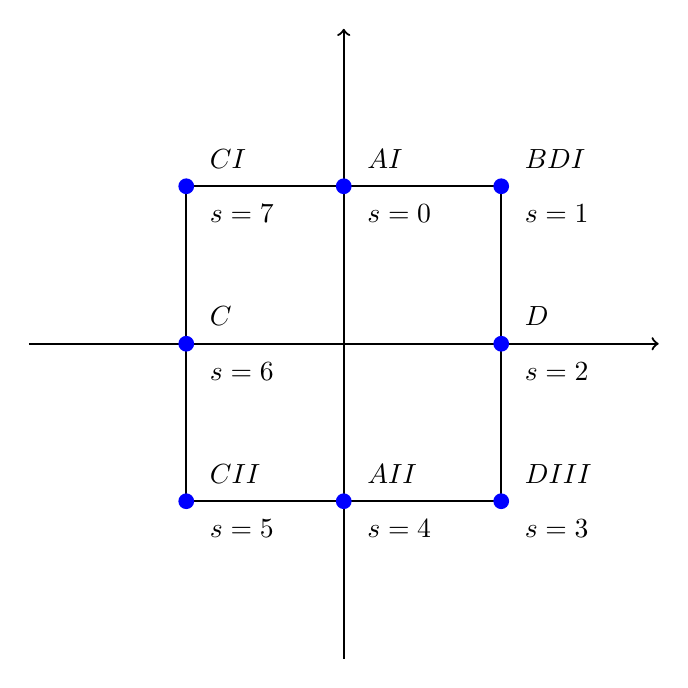
\begin{tikzpicture}
        \draw[->,thick](-4,0)--(-2,0)--(2,0)--(4,0);
        \draw[->,thick](0,-4)--(0,-2)--(0,2)--(0,4);
        \draw[thick](-2,-2)--(-2,2)--(2,2)--(2,-2)--cycle;
        \fill[blue] (0,2) circle (0.1);
        \node[above=1em,right=0.5em] at (0,2) {$AI$};
        \node[below=1em,right=0.5em] at (0,2) {$s=0$};
        \fill[blue] (2,2) circle (0.1);
        \node[above=1em,right=0.5em] at (2,2) {$BDI$};
        \node[below=1em,right=0.5em] at (2,2) {$s=1$};
        \fill[blue] (2,0) circle (0.1);
        \node[above=1em,right=0.5em] at (2,0) {$D$};
        \node[below=1em,right=0.5em] at (2,0) {$s=2$};
        \fill[blue] (2,-2) circle (0.1);
        \node[above=1em,right=0.5em] at (2,-2) {$DIII$};
        \node[below=1em,right=0.5em] at (2,-2) {$s=3$};
        \fill[blue] (0,-2) circle (0.1);
        \node[above=1em,right=0.5em] at (0,-2) {$AII$};
        \node[below=1em,right=0.5em] at (0,-2) {$s=4$};
        \fill[blue] (-2,-2) circle (0.1);
        \node[above=1em,right=0.5em] at (-2,-2) {$CII$};
        \node[below=1em,right=0.5em] at (-2,-2) {$s=5$};
        \fill[blue] (-2,0) circle (0.1);
        \node[above=1em,right=0.5em] at (-2,0) {$C$};
        \node[below=1em,right=0.5em] at (-2,0) {$s=6$};
        \fill[blue] (-2,2) circle (0.1);
        \node[above=1em,right=0.5em] at (-2,2) {$CI$};
        \node[below=1em,right=0.5em] at (-2,2) {$s=7$};
    \end{tikzpicture}
    \caption{周期性时钟}
\end{figure}
\begin{table}[h]
    \centering
    \begin{tabular}{|l|l|l|l|l|l|l|l|l|}
    \hline
    $s-\delta$ & 0   & 1           & 2           & 3 & 4    & 5 & 6 & 7 \\ \hline
    $K(s;d,D)$ & $Z$ & $Z_2^{(1)}$ & $Z_2^{(2)}$ & 0 & $2Z$ & 0 & 0 & 0 \\ \hline
    \end{tabular}
    \caption{周期表}
\end{table}

为了讨论具有拓扑非平凡态的一个可观察的结果,让我们回想一下,根据定义,如果严格执行对称条件,相图中的拓扑非平凡态和平凡态总是被量子相变分开的。这反过来意味着,如果拓扑绝缘体或拓扑超导体在空间上接近一个平凡相,那么在两相之间的边界上应该有一个无能隙的态。这种无能隙(即临界)状态可以被认为是由于空间中局部发生的相变而产生的,在这种相变中,哈密顿量的参数作为横向到边界方向的函数变化。这种无能隙边界模在这样的意义上得到了保护,即只要体隙不和对称性不被破坏,它们在扰动下是稳定的。特别是,无能隙边界模完全不受无序影响,完全规避Anderson局部化。这种无能隙边缘态的存在是拓扑绝缘体和拓扑超导体最显著的特征,实际上可以看作是拓扑绝缘体和拓扑超导体的定义。这种非平凡体拓扑性质和无能隙边模之间的紧密联系被称为体边对应

\subsubsection{拓扑缺陷}
将体拓扑绝缘体和拓扑超流体从物质的平凡态中分离出来的边界是余维1对象,即比体维数小一维,这些状态具有拓扑保护的无能隙模式。可以讨论一般更高余维的拓扑缺陷,如在能隙体系统中引入的点和线缺陷,以及它们的拓扑分类。绝热循环的拓扑性质也可以用类似的方式进行讨论。

拓扑缺陷最初是在自发对称破缺的背景下讨论的。例如,II型超导的量子通量涡旋涉及配对序参量的缠绕,打破了电荷守恒$U(1)$对称性。位错和滑移是与晶格介质中离散的扭转和曲率通量相关联的晶体缺陷,它打破了连续的平移和旋转对称性。它们都涉及缺陷周围某些序参量的非平凡长尺度调制。

拓扑带理论中的拓扑缺陷有不同的起源,因为它们不一定与自发对称破缺有关。例如,拓扑绝缘体和平凡绝缘体之间的质量间隙并不破坏任何对称。在能带理论中,它仍然是控制材料体拓扑的一个参数,我们将其称为能带参数或拓扑参数。因此,绝缘体和超导中的拓扑缺陷是缺陷周围这些拓扑参数的非平凡长尺度缠绕。

对于我们感兴趣的拓扑缺陷是由一个有缺陷的哈密顿描述的,它是一个在空间上由参量$r$缓慢调制的能带哈密顿$H_{r}(k)=H(k,r)$,其中包括空间坐标和/或时间参数。缺陷哈密顿量描述了缺陷周围的大尺度环境——距离缺陷很远。调制速度足够慢,使得与缺陷核心分离的体系统具有微观的时空平移对称性,因此可以用动量$k$来表征。更精确的讲,我们假设$\xi|\delta_rH(k,r)\leq \epsilon_h|$,其中$\xi$是类似于晶格间距或者类似于$1/\varepsilon_g$的时间微观特征长度,其中$\varepsilon_g$是能带体隙。TR、PH和CS对称性作用在缺陷哈密顿上为
\begin{equation}
    \begin{split}
        TH(k,r)T^{-1}=H(-k,r)\\
        CH(k,r)C^{-1}=-H(-k,r)\\
        SH(k,r)S^{-1}=-H(k,r)
    \end{split}
\end{equation}
其中空间参数$r$(当讨论绝热循环时是时间参数)是不变的,因为对称性作用在局域微观自由度上,它们与缓慢变化的调制无关。

不同的缺陷哈密顿可以用下列三个量来区分
\begin{enumerate}
    \item AZ对称类$s$
    \item 体维数$d$
    \item 缺陷的余维$d_c$,这是根据缺陷的维数$d_{defect}$定义的$d_c=d-d_{defect}$
\end{enumerate}
维数$d_{defect}$的空间缺陷被$D$维球面$S^{D}$包裹,其中$D=d_c-1=d-d_{defect}-1$. 例如三维空间中的一个点缺陷有余维$d_c=3-0=3$,因此被一个二维球面包络。绝热循环被合并为拓扑缺陷,依赖于循环时间参数。在这个情况下,缺陷被$S^{D-1}$球面包裹,在$d$维实空间里维数为$D-1=d-d_{defect}-1$. 算上在$S^1$上的时间参数,绝热循环被$D$维流形$S^{D-1}\times S^1$包围。

对于实AZ对称类,结果表明,拓扑缺陷的分类只依赖于一个数
\begin{equation}
    s-\delta=s-d-d_{defect}\quad mod\quad 8
\end{equation}
其中$\delta=d-D$被称为拓扑维,它在能隙拓扑绝缘体和拓扑超导的情况里扮演一个常用维数$d$的角色。对于空间缺陷,拓扑维依赖于缺陷维数$\delta=d-D=d_{defect}+1$并且与体维数$d$独立无关。例如点缺陷总有$\delta=1$,线缺陷总有$\delta=2$. 对于绝热循环,$D$分量参数$r$中的额外时间参数使拓扑维数减少1。例如,点缺陷的时间循环有$\delta=0$. 

两个复AZ类A和AIII中的拓扑缺陷以类似的方式分类,除了对称类现在存在于一个两个小时的周期时钟上,拓扑维数$\delta=d−D$以及数字$d−\delta$现在是模$2$的整数。当$\delta$是偶数(奇数),Class A(Class AIII)中的拓扑缺陷是整数类的。除此之外他们是平凡类。通过丢弃反幺正对称性,实AZ类分裂成两个复对称类
\begin{equation}
    \begin{split}
        &AI,D,AIII,C\rightarrow A\\
        &BDI,DIII,CI,CII\rightarrow AIII
    \end{split}
\end{equation}
其中手征算符$S$由TR和PH的乘积给出,这个过程依赖于实分类和复分类。例如,周期表中$s-\delta=4mod8$的$2Z$分类是根据相应的复$Z$分类归一化的。这意味着当丢弃反幺正对称时,$s−\delta=4$的拓扑不变量必须是偶数。

就像将体拓扑与边缘无能隙激发联系起来的体—边对应一样,我们也有一个体缺陷对应,它保证了体拓扑参数围绕缺陷的非平凡缠绕的无能隙缺陷激发。

\subsection{拓扑不变量}
在这一节中,我们根据体拓扑不变量讨论了能隙拓扑绝缘体和拓扑超导的十重分类和拓扑缺陷。将在下表中对讨论的拓扑不变量做简短总结。我们将讨论拓扑不变量和具有拓扑不变量特征的系统的各种具体例子,但我们主要局限于从能隙拓扑绝缘体和拓扑超导中选取的例子。拓扑缺陷的例子以后再讨论。

\begin{table}[h]
    \centering
    \begin{tabular}{|l|l|l|}
    \hline
                & Nonchiral classes(s even) & Chiral classes(s odd) \\ \hline
    $Z$         & 陈数                        & 缠绕数                   \\ \hline
    $Z_2^{(1)}$ & CS                        & Fu-Kane               \\ \hline
    $Z_2^{(2)}$ & Fu-Kane                   & CS                    \\ \hline
    \end{tabular}
    \caption{拓扑不变量分类表}
\end{table}

根据Bloch-BdG哈密顿量的本征函数给出了本节引入的拓扑不变量。我们把能级$\varepsilon^a$的本征函数记作$|u^a(k,r)\rangle$,$H(k,r)|u^a(k,r)\rangle=\varepsilon^a(k,r)|u^a(k,r)\rangle$. 通过假设,在$\varepsilon^a(k,r)$给出的能带结构中,在费米能量处存在一个能隙。我们假设在费米能量上下有$N_{+/-}$个带。总能带数为$N_++N_-$. 我们把满带Bloch函数记作$\{|u_-^\alpha(k,r)\rangle\}$或者简单记作$\{|u^\alpha(k,r)\}$,其中$\alpha=1,\cdots,N_-$.

布洛赫函数定义在$BZ^d\times\mathcal{M}^d$流形上,$(d+D)$维的总相空间由$(k,r)$参数化。这里$D$维流形$\mathcal{M}^D$围绕着这个拓扑缺陷。(它从缺陷的时空间的补形变收缩而来)例如,去掉实三维空间中的一个点缺陷,留下一个穿孔空间,该空间与$2$维球面$S^2$具有相同的同伦型。无现长线缺陷的补在三维空间中可以沿着缺陷方向压扁成一个有穿孔的盘子,然后变形回缩到圆$S^1$. 包围一个更加复杂的拓扑缺陷的$D$维流形$\mM^D$可能不会是一个球。例如,在三维空间中围绕连杆的是一个$T^2$。时间循环的流形$D$必须包含一个与周期时间方向相对应的不可收缩的1循环。本系列大部分中,我们感兴趣的是不涉及低维循环缺陷的最高维强拓扑。为此目的,通过收缩所有低维度的循环,我们将相空间紧化成一个球
\begin{equation*}
    (k,r)\in BZ^d\times\mM^D\xrightarrow{\text{紧化}}S^{d+D}
\end{equation*}
从物理上讲,这意味着缺陷能带理论假定在这些低维循环周围有平凡的缠绕。
\subsubsection{$s$为偶数的奇系:Chern数}
对于在非手征类($s$为偶数)能隙拓扑相和拓扑缺陷,整数$Z$分类的拓扑由Chern数表征
\begin{equation}
    Ch_n=\frac{1}{n!}\left(\frac{i}{2\pi}\right)^n\int_{BZ^d\times\mathcal{M}^D}Tr(\mathcal{F}^n)
\end{equation}
其中$n=(d+D)/2$. Berry曲率为
\begin{equation}
    \mathcal{F}=dA+A\wedge A
\end{equation}
这里用了微分形式:
\begin{equation}
    A^{\alpha\beta}=A_I^{\alpha\beta}(s)\mathrm{d}s^I,\quad A_I^{\alpha\beta}=\langle u^\alpha(s)|\partial_I u^\beta(s)\rangle
\end{equation}
\begin{equation}
    \begin{split}
        \mathcal{F}^{\alpha\beta}&=dA^{\alpha\beta}+A^{\alpha\gamma}\wedge A^{\gamma\beta}\\
        &=\partial_J A_I^{\alpha\beta}(s)\mathrm{d}s^J\wedge\mathrm{d}s^I+A_I^{\alpha\gamma}A_J^{\gamma\beta}\mathrm{d}s^I\wedge\mathrm{d}s^J\\
        &=\frac{1}{2}(\partial_IA_J^{\alpha\beta}(s)+[A_I^{\alpha\gamma},A_J^{\gamma\beta}])\mathrm{d}s^I\wedge \mathrm{d}s^J
    \end{split}
\end{equation}
其中$I,J=1,2,\cdots,d+D.$以及$s=(k,r)$. $A^{\alpha\beta}(k,r)$表示非阿贝尔联络
\begin{equation}
    \begin{split}
        A^{\alpha\beta}(k,r)&=\langle u^{\alpha}(k,r)|\mathrm{d}u^\beta(k,r)\rangle\\
        &=\langle u^\alpha(k,r)|\nabla_k u^\beta(k,r)\rangle\cdot \mathrm{d}k+\langle u^\alpha(k,r)|\nabla_r u^\beta(k,r)\rangle\cdot \mathrm{d}r
    \end{split}
\end{equation}
当$d+D$是偶数的时候,Chern数良定义。此外,在出现$TRS$或者$PHS$的系统里当$\delta=d-D=2\mod{4}$或者$0\mod{4}$时,Chern数为零。而且当$s-\delta=4\mod{8}$时,Chern数必定为偶数。

Chern数可以检测在底空间$BZ^d\times\mathcal{M}^D$上定义光滑Bloch波函数的障碍。与每一个$(k,r)$联系,我们有一个波函数$|u^a(k,r)\rangle$集合,一个可以被认为是$U(N_++N_-)$的一个元素的集合。然而,有一个规范冗余:对于给定的$(k,r)$在空带和占据带波函数中的$U(N_{\pm})$转动产生了相同的量子基态(费米狄拉克海)。换句话说,量子基态在给定的$(k,r)$中是陪集空间$U(N_++N_-)/U(N_-)\times U(N_+)$的一个元素,是复Grassmannian流形。费米狄拉克海可以很方便的用谱投影算符来表述
\begin{equation}
    P(k,r)=\sum_{\alpha=1}^{N_-}|u^\alpha(k,r)\rangle\langle u^\alpha(k,r)|
\end{equation}
或者写成指标显式$P^{ij}(k,r)=\sum_{\alpha=1}^{N_-}u_i^\alpha(k,r)[u_j^\alpha(k,r)]^*$,它指定了一个由占据带的布洛赫波函数的集合定义的总希尔伯特空间的子空间。投影算符是规范不变的并且是复Grassmannian流形的一个元素$P(k,r)\in U(N_++N_-)/(U(N_-)\times U(N_+))$. 对于下面的内容,引入$Q$矩阵是很方便的
\begin{equation}
    Q(k,r)=1-2P(k,r)
\end{equation}
$Q$矩阵是厄米的并且和$H(k,r)$有相同的本征函数集,但是他的本征值是$\pm 1$,因为$Q^2=1$.

当我们在底空间$BZ^d\times \mathcal{M}^D$移动的时候,波函数集合发生绝热变化。这样的波函数就定义了一个可以“扭曲”的纤维丛:在底空间各处都要找到定义良好的光滑波函数可能是不可能的。一个查看纤维丛什么时候扭曲的快速方法是注意到布洛赫函数的集合定义了一个从底空间到$U(N_++N_-)/(U(N_+)\times U(N_-))$的映射。这类拓扑上不同的映射可以用同伦群来分类
\begin{equation}
    \pi_{d+D}[U(N_++N_-)/(U(N_+)\times U(N_-))]
\end{equation}
对于足够大的$N_\pm$以及$d+D$是偶数的时候,$\pi_{d+D}[U(N_++N_-)/(U(N_+)\times U(N_-))]=Z$. 因此,拓扑上不同的映射具有整数拓扑不变量的特征,即
\begin{equation}
    -\frac{1}{2^{2n+1}}\frac{1}{n!}\left(\frac{i}{2\pi}\right)^n\int_{BZ^d\times \mathcal{M}^D}Tr[Q(\mathrm{d}Q)^{2n}]
\end{equation}
这不是什么,这正是Chern数。
\paragraph{例子:二维Class A量子反常霍尔效应}
作为一个例子,我们考虑$N_+=N_-=1$维数为$2$的带绝缘体。一般而言,二带布洛赫哈密顿可以根据四个实函数$R_{0,1,2,3}(k)$写成
\begin{equation}
    H(k)=R_0(k)\sigma_0+\mathbf{R}(k)\cdot \mathbf{\sigma}
\end{equation}
其中$\mathbf{R}=(R_1,R_2,R_3)$. 能带的能量色散关系为
\begin{equation}
    \varepsilon_{\pm}(k)=R_0(k)\pm R(k),\quad R(k)=|\mathbf{R}(k)|
\end{equation}
对于带绝缘体,在费米能处有一个能隙,为了方便起见,令此处的能量为$0$. 因此我们假设$R_0(k)+R(k)>0>R_0(k)-R(k)$,特别地,这意味着对于所有$k$都有$R(k)>0$

在这个二带的粒子里,布洛赫哈密顿$H(k)$或者四个矢量$R_{\mu=0,1,2,3}(k)$定义了从BZ到无约束四维向量$R_\mu$空间的映射。然而布洛赫波函数仅仅依赖单位矢量$\mathbf{n}(k)=\mathbf{R}(k)/R(k)$,这从以下两点很容易看到:
\begin{enumerate}
    \item $H(k)$中的$R_0(k)$并不会影响到波函数
    \item $\mathbf{R}(k)\cdot\mathbf{\sigma}=R(k)\mathbf{n}(k)\cdot\mathbf{\sigma}$
\end{enumerate}
从布洛赫波函数的这个观点出发,我们考虑一个从BZ到$S^2$上单位矢量$\mathbf{n}$的映射。后者是复Grassmannian流形的最简单的例子$U(2)/U(1)\times U(1)=S^2$

在二带模型中,不同的带绝缘体可以被不同的映射$\mathbf{n}(k)$表征。通过把BZ$T^2$紧化为$S^2$,拓扑上不同的映射可以利用二阶同伦群$\pi_2(S^2)$来分类,这给出了$\pi_2(S^2)=Z$. 对于给定的映射$\mathbf{n}$,整数拓扑不变量为
\begin{equation}\label{Chern num2}
    \frac{1}{4\pi}\int_{BZ}\mathbf{n}\cdot\mathrm{d}\mathbf{n}\times\mathrm{d}\mathbf{n}\in Z
\end{equation}
这可以计算出当我们扫过BZ时单位向量$\mathbf{n}$缠绕$S^2$的次数并且告诉我们$n$映射属于哪一个拓扑类。

现在让我们明确地构造布洛赫波函数。一个可能的选择是
\begin{equation}\label{wavefun1}
    |u^{\pm}\rangle=\frac{1}{\sqrt{2R(R\mp R_3)}}\begin{pmatrix}
        R_1-iR_2\\
        \pm R-R_3
    \end{pmatrix}
\end{equation}
观察占据带布洛赫函数$|u^-\rangle$在$\mathbf{R}=(0,0,-R)$处有一个奇点。当拓扑不变量\eqref{Chern num2}是非零的时候,矢量$\mathbf{n}(k)$必然将BZ中至少一个点映射到南极,因此,如果坚持在BZ中处处使用波函数\eqref{wavefun1},就会遇到奇点。从这个意义上说,在定义BZ中全局光滑良好的波函数时存在一个障碍。为了避免这个奇异性,我们可以把BZ分片,并且在不同片上用不同的波函数。例如在南极附近我们可以选择
\begin{equation}\label{wavefun2}
    |u^\pm\rangle=\frac{1}{\sqrt{2R(R\pm R_3)}}\begin{pmatrix}
        \pm R+R_3\\
        R_1+i R_2
    \end{pmatrix}
\end{equation}
这个波函数在南极是光滑的,但是在北极$\mathbf{R}=(0,0,R)$处是奇异的。利用两片波函数可以覆盖整个BZ。在两片交叠区域,两个波函数通过规范变换联系起来。

利用布洛赫波函数的显式形式,我们可以计算谱投影算符或者$Q$矩阵,并且可以看到不同的规范选择\eqref{wavefun1}和\eqref{wavefun2}产生相同的投影算符(投影算符规范不变),并且仅仅只依赖于$\mathbf{n}(k)$.

例如我们选择规范\eqref{wavefun1}
\begin{equation*}
    \begin{split}
        P&=|u^-\rangle\langle u^-|=\frac{1}{2R(R+R_3)}\begin{pmatrix}
            R_1-iR_2\\
            -R-R_3
        \end{pmatrix}\begin{pmatrix}
            R_1+iR_2&-R-R_3
        \end{pmatrix}\\
        &=\begin{pmatrix}
            \frac{R_1^2+R_2^2}{2R(R+R_3)}&-\frac{R_1-iR_2}{2R}\\
            -\frac{R_1+iR_2}{2R}&\frac{(R+R_3)^2}{2R(R+R_3)}
        \end{pmatrix}
    \end{split}
\end{equation*}
这样可以计算出$Q$矩阵
\begin{equation}
    Q=1-2P=\begin{pmatrix}
        \frac{R_3}{R}&\frac{R_1-iR_2}{R}\\
        \frac{R_1+iR_2}{R}&-\frac{R_3}{R}
    \end{pmatrix}=\frac{\mathbf{R}\cdot \bm{\sigma}}{R}
\end{equation}
Chern数为
\begin{equation*}
    \begin{split}
        Ch^1&=-\frac{i}{16\pi}\int_{BZ}Tr[Q\mathrm{d}Q\wedge \mathrm{d}Q]\\
        &=-\frac{i}{16\pi}\int_{BZ}Tr[Q(\frac{\partial Q}{\partial k_x}\frac{\partial Q}{\partial k_y}-\frac{\partial Q}{\partial k_y}\frac{\partial Q}{\partial k_x})]\mathrm{d}k_x\wedge \mathrm{d}k_y\\
        &=-\frac{i}{16\pi}\int_{BZ}Tr[\bm{\sigma}\cdot\mathbf{n}(\bm{\sigma}\cdot\frac{\partial\mathbf{n}}{\partial k_x}\bm{\sigma}\cdot\frac{\partial\mathbf{n}}{k_y}-\bm{\sigma}\cdot\frac{\partial\mathbf{n}}{\partial k_y}\bm{\sigma}\cdot\frac{\partial\bm{n}}{\partial k_x})]\mathrm{d}k_x\wedge\mathrm{d}k_y
    \end{split}
\end{equation*}
分为两项分别计算
\begin{equation}
    \begin{split}
        Term1&=\sigma_i n_i\sigma_j\frac{\partial n_j}{\partial k_x}\sigma_k\frac{\partial n_k}{\partial k_y}\\
        &=(\delta_{ij}+i\varepsilon_{ijk'}\sigma_{k'})\sigma_kn_i\frac{\partial n_j}{\partial k_x}\frac{\partial n_k}{\partial k_y}\\
        &=\sigma_k n_i\frac{\partial n_i}{\partial k_x}\frac{\partial n_k}{k_y}+i\varepsilon_{ijk}n_i\frac{\partial n_j}{\partial k_x}\frac{\partial n_k}{\partial k_y}-(\delta_{ki}\delta_{lj}-\delta_{kj}\delta_{li})\sigma_ln_i\frac{\partial n_j}{\partial k_x}\frac{\partial n_k}{\partial k_y}\\
        &=\mathbf{n}\cdot\frac{\partial\mathbf{n}}{\partial k_x}(\bm{\sigma}\cdot\frac{\partial\mathbf{n}}{\partial k_y})+i\varepsilon_{ijk}n_i\frac{\partial n_j}{\partial k_x}\frac{\partial n_k}{\partial k_y}-(\mathbf{n}\cdot\frac{\partial\mathbf{n}}{\partial k_y})(\bm{\sigma}\cdot\frac{\partial\mathbf{n}}{\partial k_x})+(\bm{\sigma}\cdot\mathbf{n})(\frac{\partial\mathbf{n}}{\partial k_x}\cdot\frac{\partial\mathbf{n}}{\partial k_y})\\
        Term2&=Term1(x\leftrightarrow y)
    \end{split}
\end{equation}
所以Chern数为(注意这里要Trace一个单位矩阵会多一个$2$倍)
\begin{equation}
    Ch^1=\frac{1}{8\pi}\int_{BZ}\mathbf{n}\cdot(\mathrm{d}\mathbf{n}\times\mathrm{d}\mathbf{n})
\end{equation}
利用Bloch波函数,我们可以计算Berry联络和Chern数,同样也可以得到上面的结果

这里展示一下计算过程,为了方便,我们依旧选取规范\eqref{wavefun1},因为规范的选取并不影响Berry Curvature的结果。这次我们在$\mathbf{R}$所在的$S^2$作为底流形上计算:
\begin{equation}
    \begin{split}
        Ch^1&=\frac{i}{2\pi}\int_{BZ}Tr(F)=\frac{i}{2\pi}\int_{BZ}Tr(\frac{1}{2}F_{\mu\nu}^{\alpha\beta}\mathrm{d}R^\mu\wedge\mathrm{d}R^{\nu})\\
        &=\frac{i}{4\pi}\int_{BZ}Tr(F_{\mu\nu}^{\alpha\beta})\mathrm{d}R^\mu\wedge\mathrm{d}R^\nu\\
        &=\frac{i}{4\pi}\sum_{\alpha}\int_{BZ}F_{\mu\nu}^{\alpha\alpha}\mathrm{d}R^\mu\wedge\mathrm{d}R^\nu\\
        &=\frac{i}{4\pi}\sum_{\alpha\beta}\int_{BZ}\frac{\langle u^\alpha|\partial_\mu H|u^\beta\rangle\langle u^\beta|\partial_\nu H|u^\alpha\rangle}{(E^\alpha-E^\beta)^2}\mathrm{d}R^\mu\wedge\mathrm{d}R^\nu\\
        &=\frac{i}{4\pi}\sum_{\alpha\beta}\int_{BZ}\frac{\langle u^\alpha|\sigma_\mu|u^\beta\rangle\langle u^\beta|\sigma_\nu|u^\alpha\rangle}{(E^\alpha-E^\beta)^2}\mathrm{d}R^\mu\wedge\mathrm{d}R^\nu
    \end{split}
\end{equation}
Chern数的Trace仅仅对占满的能带求和
\begin{equation}
    \begin{split}
        Ch^1&=\frac{i}{4\pi}\int_{S^2}\frac{\langle u^-|\sigma_i|u^+\rangle\langle u^+|\sigma_j|u^-\rangle}{(E^--E^+)^2}\mathrm{d}R^i\wedge\mathrm{d}R^j\\
        &=\frac{i}{4\pi}\int_{S^2}\frac{\langle u^-|i\varepsilon_{ijk}\sigma_k|u^-\rangle-\langle u^-|\sigma_i|u^-\rangle\langle u^-|\sigma^j|u^-\rangle}{4R^2}\mathrm{d}R^i\wedge\mathrm{d}R^j\\
        &=\frac{i}{4\pi}\int_{S^2}\frac{i\varepsilon_{ijk}R^k}{4R^3}\mathrm{d}R^i\wedge\mathrm{d}R^j\\
        &=\frac{i}{4\pi}\int_{S^2}\frac{i}{4}\varepsilon_{ijk}n^k\mathrm{d}n^i\wedge\mathrm{d}n^j\\
        &=\frac{i}{4\pi}\int_{BZ}\frac{i}{4}\varepsilon_{ijk}n^i(\frac{\partial n^i}{\partial k^\mu}\frac{\partial n^j}{\partial k^\nu}-\frac{\partial n^i}{\partial k^\nu}\frac{\partial n^j}{\partial k^\mu})\mathrm{d}k^\mu\wedge\mathrm{d}k^\nu\\
        &=\frac{i}{4\pi}\int_{BZ}\frac{i}{2}\varepsilon_{ijk}n^i(\partial_\mu n^i)(\partial_\nu n^j)\mathrm{d}k^\mu\wedge\mathrm{d}k^\nu
    \end{split}
\end{equation}
所以我们可以看到Berry Curvature为
\begin{equation}
    Tr(\mathcal{F}(\mathbf{k}))=\frac{i}{2}\varepsilon_{ijk}n^i(\partial_\mu n^i)(\partial_\nu n^j)\mathrm{d}k^\mu\wedge\mathrm{d}k^\nu
\end{equation}
这与之前用$Q$矩阵计算结果一样

二带模型非零Chern数的一个很显然的例子是
\begin{equation}
    \mathbf{R}(k)=\begin{pmatrix}
        -2\sin k_x\\
        -2\sin k_y\\
        \mu+2\sum_{i=x,y}\cos k_i
    \end{pmatrix}
\end{equation}
\begin{equation}
    H=\mathbf{R}\cdot \bm{\sigma}=\begin{pmatrix}
        \mu+2\sum_{i=x,y}\cos{k_i}&-2\sin k_x+2i\sin k_y\\
        -2\sin k_x-2i\sin k_y&-\mu-2\sum_{i=x,y}\cos k_i
    \end{pmatrix}
\end{equation}
分别有三个量子相变点,分别在$\mu=0,\pm 4$,对应有四个相,Chern数分别为
\begin{equation}
    Ch=\begin{cases}
        0\quad&(|\mu|>4)\\
        -1\quad&(-4<\mu<0)\\
        1\quad&(0<\mu<4)
    \end{cases}
\end{equation}
$d=2$维晶格上Chern数非零且无净磁场的带绝缘体通常称为Chern绝缘体,并表现出量子反常霍尔效应,这推广了在存在均匀磁场下的整数霍尔效应。Chern数不是什么别的,正是量子霍尔电导$\sigma_{xy}$.

\subsubsection{s为奇数的基础系:缠绕数}
对于Bloch-BdG哈密顿,只要$d+D$为偶数,Chern数总是可以被定义的(尽管它的允许值取决于对称类和δ)。另一方面,拓扑不变量只有在对称存在的情况下才能定义。一个例子是拓扑不变量缠绕数$\nu$,它仅仅在手征对称($\{H(k,r),U_S\}=0,U_S^2=1$)出现的情况下才能定义。简单起见,我们关注于$TrU_S=0$的情况,例如$N_+=N_-=N$.在不存在手性对称性的情况下,投影算符是复Grassmannian的一个元素,而在存在手性对称性的情况下,相关的空间是酉群$U(N)$. 这点可以从手征对称哈密顿的反对角形式看到
\begin{equation}
    H(k,r)=\begin{pmatrix}
        0&D(k,r)\\
        D^\dagger(k,r)&0
    \end{pmatrix}
\end{equation}
对应的,在这个基里,$Q$矩阵也是反对角的
\begin{equation}
    Q=1-2P(k,r)=\begin{pmatrix}
        0&q(k,r)\\
        q^\dagger(k,r)&0
    \end{pmatrix}
\end{equation}
这里稍微证明一下

选取$H$的一个基底$|u\rangle$满足$H|u\rangle=\varepsilon|u\rangle$,由于手征对称并且$TrU_S=0$,每一个能级$\varepsilon$的$|u\rangle$都有一个能量$-\varepsilon$的$U_S|u\rangle$对应。我们知道
\begin{equation}
    \begin{split}
        U_S|\alpha\rangle&=|\alpha\rangle\\
        U_S|\beta\rangle&=-|\beta\rangle
    \end{split}
\end{equation}
其中$|\alpha\rangle=|u\rangle+U_S|u\rangle,|\beta\rangle=|u\rangle-U_S|u\rangle$

这样我们可以到从$H$对角表象到CS表象下的变换关系
\begin{equation}
    \begin{split}
        |u\rangle=\frac{1}{2}(|\alpha\rangle+|\beta\rangle)\\
        |U_Su\rangle=\frac{1}{2}(|\alpha\rangle-|\beta\rangle)
    \end{split}
\end{equation}
计算$Q$矩阵得到
\begin{equation}
    Q=|U_Su\rangle\langle U_Su|-|u\rangle\langle u|=-\frac{1}{2}(|\alpha\rangle\langle\beta|-|\beta\rangle\langle\alpha|)=\begin{pmatrix}
        0&q(k,r)\\
        q^\dagger(k,r)&0
    \end{pmatrix}
\end{equation}
其中反对角块$q(k,r)$是一个幺正矩阵。因此$q$矩阵定义了一个从底流形$BZ^d\times \mathcal{M}^D$到李群流形$U(N)$的映射。拓扑上区分这类映射是用同伦群$\pi_{d+D}(U(N))$分类,这个同伦群在$d+D$为奇数时是非平凡的,例如$\pi_{d+D}[U(N)]=\mathbf{Z}$($N$足够大)。拓扑不同的映射是用缠绕数来表征的
\begin{equation}
    \begin{split}
        \nu_{2n+1}[q]&=\int_{BZ^d\times\mathcal{M}^D}\omega_{2n+1}[q]\\
        \omega_{2n+1}[q]&=\frac{(-1)^nn!}{(2n+1)!}\left(\frac{i}{2\pi}\right)^{n+1}Tr[(q^{-1}\mathrm{d}q)^{2n+1}]
    \end{split}
\end{equation}
其中$d+D=2n+1$是奇数。例如当$(d,D)=(1,0),(3,0)$我们有
\begin{equation}
    \begin{split}
        \nu_1&=\frac{i}{2\pi}\int_{BZ}\mathrm{d}kTr[q^{-1}\partial_k q]\\
        \nu_3&=\int_{BZ}\frac{\mathrm{d}^3k}{24\pi^2}\varepsilon^{\mu\nu\rho}Tr[(q^{-1}\partial_\mu q)(q^{-1}\partial_\nu q)(q^{-1}\partial_\rho q)]
    \end{split}
\end{equation}
这里$\partial_\mu=\partial_{k_\mu}$
\subsubsection{s为奇数的基础系:Chern-Simons}
我们现在引入另一个拓扑不变量,Chern-Simons不变量。这个不变量可以在$d+D=$奇数时定义,并且不像Chern数是量子化的。然而,在对称性存在的情况下,它可以取离散值。我们随后使用量化的CS不变量来描述第一代$Z_2$和第二代$Z_2$。这里我们看到$CS$不变量在出现手征对称性时也是量子化的。

Chern-Simons不变量由$d+D=2n+1$维里Chern-Simons形式$Q_{2n+1}$定义
\begin{equation}
    \mathcal{Q}_{2n+1}=\frac{1}{n!}\left(\frac{i}{2\pi}\right)^{n+1}\int_{0}^{1}Tr(\mathcal{AF}_{t}^n),\quad F_t=t\mathrm{d}\mathcal{A}+t^2\mathcal{A}^2=t\mathcal{F}+(t^2-t)\mathcal{A}^2
\end{equation}
对Chern-Simons形式在底流形上积分得到Chern-Simons不变量
\begin{equation}
    CS_{2n+1}[\mathcal{A}]=\int_{BZ^d\times\mathcal{M}^D}\mathcal{Q}_{2n+1}(\mathcal{A})
\end{equation}
例如对于$n=0,1,2$
\begin{equation}
    \begin{split}
        \mathcal{Q}_1(\mathcal{A})&=\frac{i}{2\pi}\int_0^1\mathrm{d}tTr(\mathcal{A})=\frac{i}{2\pi}Tr(\mathcal{A})\\
        \mathcal{Q}_3(\mathcal{A})&=\left(\frac{i}{2\pi}\right)^{2}\int_0^1\mathrm{d}tTr(\mathcal{A}(t\mathrm{d}\mathcal{A}+t^2\mathcal{A}^2))=-\frac{1}{4\pi^2}Tr(\frac{1}{2}\mathcal{A}\mathrm{d}\mathcal{A}+\frac{1}{3}\mathcal{A}^3)=-\frac{1}{8\pi^2}Tr(\mathcal{A}\mathrm{d}\mathcal{A}+\frac{2}{3}\mathcal{A}^3)\\
        \mathcal{Q}_5(\mathcal{A})&=\frac{1}{2}\left(\frac{i}{2\pi}\right)^3\int_0^1Tr(\mathcal{A}(t\mathrm{d}\mathcal{A}+t^2\mathcal{A}^2)^2)=-\frac{i}{16\pi^3}\int_0^1Tr(t^2\mathcal{A}(\mathrm{d}\mathcal{A})^2+2t^3\mathcal{A}^3\mathrm{d}\mathcal{A}+t^4\mathcal{A}^5)\\
        &=-\frac{i}{16\pi^3}Tr(\frac{1}{3}\mathcal{A}(\mathrm{d}A)^2+\frac{1}{2}\mathcal{A}^3\mathrm{d}\mathcal{A}+\frac{1}{5}\mathcal{A}^5)=-\frac{i}{48\pi^3}Tr(\mathcal{A}(\mathrm{d}\mathcal{A})^2+\frac{3}{2}\mathcal{A}^2\mathrm{d}\mathcal{A}+\frac{3}{5}\mathcal{A}^5)
    \end{split}
\end{equation}
Chern-Simons形式不是规范不变的。Chern-Simons的积分形式也不是。但是对于两个不同的规范选择$A$和$A^g$,它们由一个规范变换$g$连接
\begin{equation}
    A^g=g^{-1}Ag+g^{-1}\mathrm{d}g,\quad \mathcal{F}^g=g^{-1}\mathcal{F}g
\end{equation}
Chern-Simons形式的差$\mathcal{Q}_{2n+1}(A^g)-\mathcal{Q}_{2n+1}(A)$由缠绕数密度$\omega_{2n+1}[g]$和一个全导数项给出
\begin{equation}
    \mathcal{Q}_{2n+1}(A^g)-\mathcal{Q}_{2n+1}(A)=\omega_{2n+1}[g]+\mathrm{d}\alpha_{2n+1}(A,g)
\end{equation}
这样对于Chern-Simons形式的积分
\begin{equation}\label{CS integer}
    CS_{2n+1}[A^g]-CS_{2n+1}[A]=integer
\end{equation}
并且指数形式
\begin{equation}
    W_{2n+1}=\exp(2\pi i CS_{2n+1}[A])
\end{equation}
是良定义的,规范不变的量,虽然他不必要是量子化的。

到目前为止,讨论都是泛泛的。我们现在计算了手征对称存在下的CS不变。为此,我们首先明确地写下手征对称哈密顿量的Berry联络。对于给定的$q(k,r)$,本征函数可以显式的构造为
\begin{equation}
    |u^\alpha_\epsilon(k,r)\rangle_N=\frac{1}{\sqrt{2}}\begin{pmatrix}
        |n^\alpha\rangle\\
        \epsilon q^\dagger(k,r)|n^\alpha\rangle
    \end{pmatrix},\quad \epsilon=\pm
\end{equation}
在这个构造里,$Q$矩阵是对角的,对角元分别是$1,-1$. $|n^\alpha\rangle$是$N$个正交无关向量。为了简单,我们选择$(n^\alpha)_\beta=\delta_{\alpha\beta}$. 这些波函数没有任何奇异性,也就是说,我们明确地证明了整体的构造本征波函数没有障碍。Berry联络为
\begin{equation}
    \begin{split}
        A_N&=\langle u_\epsilon^\alpha|\mathrm{d}u_\epsilon^\alpha\rangle\\
        &=\frac{1}{2}\left[\langle n^\alpha|\mathrm{d}n^\alpha\rangle+\langle q^\dagger n^\alpha|\mathrm{d}q^\dagger n^\alpha\rangle+\langle q^\dagger n^\alpha|q^\dagger \mathrm{d}n^\alpha\rangle\right]\\
        &=\langle n^\alpha|\mathrm{d}n^\alpha\rangle+\frac{1}{2}\langle n^\alpha|q\mathrm{d}q^\dagger|n^\alpha\rangle=\frac{1}{2}q\mathrm{d}q^\dagger
    \end{split}
\end{equation}
在这个规范下,CS形式$\mathcal{Q}_{2n+1}$是缠绕数的一半,$\mathcal{Q}_{2n+1}(A_N)=\omega_{2n+1}[q^\dagger]/2$. 我们可以得到$CS_{2n+1}[A_N]=\nu_{2n+1}[q^\dagger]/2$
\begin{equation}
    W_{2n+1}=\exp(\pi i\nu_{2n+1}[q])=\pm 1
\end{equation}
也就是说,对于具有手征对称的哈密顿$W_{2n+1}$仅仅能取两个值$W_{2n+1}=\pm 1$

当$(d,D)=(1,0)$时,CS不变量$W_1$是定义在$BZ^d\simeq S^1$上的$U(1)$Wilson圈。$W_1$的对数表示电子极化,可以被手征对称性和反演对称性量子化。在这种情况下,$CS_1[A]$, \eqref{CS integer}的非不变性与这样一个事实有关:在周期系统中,电子坐标的位移只在一个单元内有意义,也就是说,两个坐标相差晶格常数的整数倍,应该是恒等的。

当$(d,D)=(3,0)$时,$CS_3$表示量子化的电磁极化率或者$\theta$角。$\theta$角,用Chern-Simons积分表示为
\begin{equation}
    \theta=2\pi\int_{BZ}\mathcal{Q}_3(k)\mod{2\pi}
\end{equation}
通过轴项$\delta S=(\frac{\theta\alpha}{4\pi})\int\mathrm{d}^3r\mathrm{d}t\mathbf{E}\cdot\mathbf{B}$出现在电动力学的有效作用中,其中$\alpha$是精细结构常数。量化的磁电极化率首先是在三维TR对称拓扑绝缘体$Class AII$的背景下被注意到的。除了TRS,手征对称和反演对称也能量子化CS不变量量$W_3$
\paragraph{例子:一维Class AIII聚合物}
考虑一个一维晶格上双粒子hopping模型
\begin{center}
    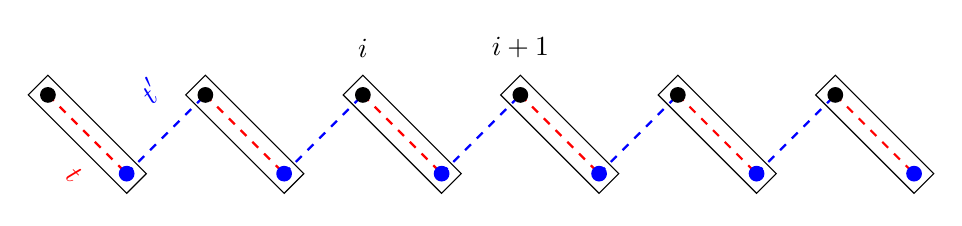
\begin{tikzpicture}
        \draw (-0.25,0) -- (1,-1.25) -- (1.25,-1) -- (0,0.25) -- cycle;
        \draw (1.75,0) -- (3,-1.25) -- (3.25,-1) -- (2,0.25) -- cycle;
        \draw (3.75,0) -- (5,-1.25) -- (5.25,-1) -- (4,0.25) -- cycle;
        \draw (5.75,0) -- (7,-1.25) -- (7.25,-1) -- (6,0.25) -- cycle;
        \draw (7.75,0) -- (9,-1.25) -- (9.25,-1) -- (8,0.25) -- cycle;
        \draw (9.75,0) -- (11,-1.25) -- (11.25,-1) -- (10,0.25) -- cycle;
        \draw[dashed,thick,red] (0,0) --node[below=1em,rotate=-45]{$t$} (1,-1);
        \draw[dashed,thick,red] (2,0) -- (3,-1);
        \draw[dashed,thick,red] (4,0) -- (5,-1);
        \draw[dashed,thick,red] (6,0) -- (7,-1);
        \draw[dashed,thick,red] (8,0) -- (9,-1);
        \draw[dashed,thick,red] (10,0) -- (11,-1);
        \draw[dashed,thick,blue] (1,-1) --node[above=1em,rotate=45]{$t'$} (2,0);
        \draw[dashed,thick,blue] (3,-1) -- (4,0);
        \draw[dashed,thick,blue] (5,-1) -- (6,0);
        \draw[dashed,thick,blue] (7,-1) -- (8,0);
        \draw[dashed,thick,blue] (9,-1) -- (10,0);
        \fill (0,0) circle (0.1);
        \fill (2,0) circle (0.1);
        \fill (4,0)node[above=1em]{$i$} circle (0.1);
        \fill (6,0)node[above=1em]{$i+1$} circle (0.1);
        \fill (8,0) circle (0.1);
        \fill (10,0) circle (0.1);
        \fill[blue] (1,-1) circle (0.1);
        \fill[blue] (3,-1) circle (0.1);
        \fill[blue] (5,-1) circle (0.1);
        \fill[blue] (7,-1) circle (0.1);
        \fill[blue] (9,-1) circle (0.1);
        \fill[blue] (11,-1) circle (0.1);
    \end{tikzpicture}
\end{center}
\begin{equation}
    \hat{H}=t\sum_{i}(a_i^\dagger b_i+h.c.)-t'\sum_{t}(b_i^\dagger a_{i+1}+h.c.)
\end{equation}
其中$a_i/b_i$是费米子在子格$A/B$上第$i$个原胞的湮灭算符。我们只考虑最近邻的hopping振幅为实数的情况,我们分别记作$t,t'$,其中我们假设$t,t'>0$. 这是描述乙炔的SSH模型。在动量空间中,哈密顿写成$\hat{H}=\sum_{k}\Psi^\dagger(k) H(k)\Psi(k)$, 其中$\Psi(k)=(a_k,b_k)^T,k\in[-\pi,\pi]$
\begin{equation}\label{lattice model}
    H(k)=\mathbf{R}(k)\cdot\bm{\sigma},\quad \mathbf{R}(k)=\begin{pmatrix}
        t-t'\cos k\\
        -t'\sin k\\
        0
    \end{pmatrix}
\end{equation}
能谱为$\varepsilon(k)=\pm\sqrt{t^2-2tt'\cos k+t'^2}$. 哈密顿有手征对称性,在动量空间里满足变换条件$\sigma_3 H\sigma_3=-H(k)$. 在这个对称性里,两个有能隙相$t>t'$和$t<t'$是拓扑可分辨的,并且被$t=t'$的量子相变点隔开。在$t>t'$相里的基态和原子绝缘体是绝热连通的。换句话说,一旦手征对称性引入,在$t'>t$相的基态与拓扑平凡原子绝缘体是拓扑区分的。这两个相由缠绕数来表征
\begin{equation}
    \nu[q]=\frac{i}{2\pi}\int_{BZ}\mathrm{d}k q^\dagger\partial_k q=\begin{cases}
        1,\quad t'>t\\
        0,\quad t'<t
    \end{cases}
\end{equation}
其中$q(k)=(t-t'e^{-ik})/|\varepsilon(k)|$. 简单计算一下
\begin{equation}
    \nu[q]=\frac{i}{2\pi}\int_{BZ}q^\dagger\mathrm{d}q=\frac{i}{2\pi}\int_{-\pi}^{\pi}\mathrm{d}k\partial_k\ln q=\left.\frac{i}{2\pi}\ln q\right|_{-\pi}^\pi
\end{equation}
\begin{equation}
    \ln q=\ln |q|+\arg q=\arg q,\quad |q|=1
\end{equation}
\begin{center}
    \begin{tikzpicture}
        \draw[->](-1,0)--(4,0);
        \draw[->](0,-2)--(0,2);
        \draw[blue] (2,0)circle(1);
        \draw (2,-0.1)node[below]{$t$}--(2,0.1);
        \draw[->](2,0)--(2.707,0.707)node[above]{$t'e^{-ik}$};
        \node[below=1em,left=0.5em] at (0,0) {$O$};
    \end{tikzpicture}
\end{center}
相应的CS不变量也有两个可区分的量子化值$1(0)$,分别对应$t'>t$和$t>t'$. 假设$t/t'$在相变点附近,SSH模型的低能物理是连续狄拉克哈密顿
\begin{equation}
    H(k)=-t'k\sigma_2+(t-t')\sigma_1
\end{equation}
这由$k$空间中的哈密顿在$k=0$处展开得到。注意到$t-t'$扮演着质量$m$的角色。

为了讨论domain wall,我们可以令$t\rightarrow t+m,t'\rightarrow t$. 更进一步说,我们让$m$是独立的,它定义了Class AIII和BDI哈密顿的一个缺陷
\begin{equation}
    H(k,r)=[t(1-\cos k)+m(r)]\sigma_1-t\sin k\sigma_2
\end{equation}
我们考虑一个受到空间调制的质量隙$m(r)$,它描述了一个domain wall的夹层,例如$m(r)=sgn(r)m_0,(|r|>R_0),m_0\neq 0$. 缠绕数为
\begin{equation}
    \begin{split}
        \nu_1&=\frac{i}{2\pi}\int_{BZ\times S^0}q^\dagger\mathrm{d}q\\
    \end{split}
\end{equation}
简单计算一下:
\begin{equation}
    H(k,r)=\mathbf{d}\cdot \sigma=\begin{pmatrix}
        &d_1-id_2\\
        d_1+id_2&
    \end{pmatrix}
\end{equation}
能量本征方程为
\begin{equation}
    \begin{pmatrix}
        &d_1-id_2\\
        d_1+id_2&
    \end{pmatrix}\begin{pmatrix}
        \alpha\\
        \beta
    \end{pmatrix}=\pm d\begin{pmatrix}
        \alpha\\
        \beta
    \end{pmatrix}
\end{equation}
\begin{equation}
    |u^\pm\rangle=\frac{1}{\sqrt{2}}\begin{pmatrix}
        \frac{d_1-id_2}{d}\\
        \pm 1
    \end{pmatrix}
\end{equation}
\begin{equation}
    Q=|u^+\rangle\langle u^+|-|u^-\rangle\langle u^-|=\begin{pmatrix}
        &\frac{d_1-id_2}{d}\\
        \frac{d_1+id_2}{d}&
    \end{pmatrix},\quad q=\frac{d_1-id_2}{d}
\end{equation}
\begin{equation}
    \begin{split}
        \nu_1&=\frac{i}{2\pi}\int_{BZ\times S^0}q^\dagger dq\\
        &=\frac{i}{2\pi}\int_{BZ}\mathrm{d}k[q^\dagger(k,R_0)\partial_k q(k,R_0)-q^\dagger(k,-R_0)\partial_k q(k,-R_0)]\\
        &=-\frac{1}{2\pi}[\arg q(k,R_0)|_0^{2\pi}-\arg q(k,-R_0)|_0^{2\pi}]
    \end{split}
\end{equation}
\begin{equation}
    d_1=t+m(r)-t\cos k,\quad d_2=-t\sin k,\quad d_1-id_2=t+m(r)-te^{-ik}
\end{equation}
\begin{center}
    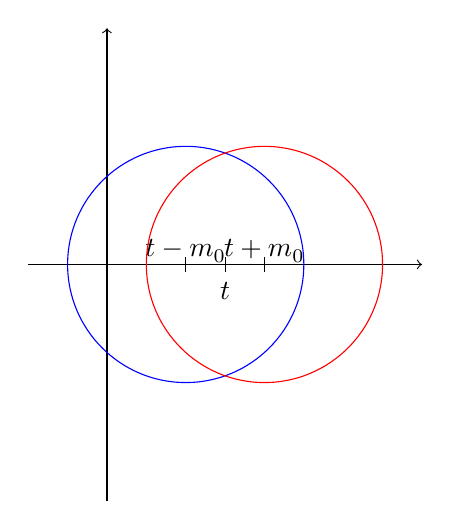
\begin{tikzpicture}
        \draw[->](-1,0)--(4,0);
        \draw[->](0,-3)--(0,3);
        \draw[blue](1,0)circle(1.5);
        \draw(1,-0.1)node[above]{$t-m_0$}--(1,0.1);
        \draw[red](2,0)circle(1.5);
        \draw(2,-0.1)node[above]{$t+m_0$}--(2,0.1);
        \draw(1.5,-0.1)node[below]{$t$}--(1.5,0.1);
    \end{tikzpicture}
\end{center}
其中$S^0=\{R_0,-R_0\}$是在原点处夹着缺陷点的两个点。该缺陷还以CS积分为特征,在这个例子里是电极化率
\begin{equation}
    CS_1=\frac{i}{2\pi}\int_{BZ\times S^0}\mathcal{A}=\frac{i}{2\pi}\int_{0}^{2\pi}\mathrm{d}k[A(k,R_0)-A(k,-R_0)]
\end{equation}
\begin{equation}
    A=\langle u^-|\partial_k|u^-\rangle=\frac{i}{2}\partial_k\ln q
\end{equation}
所以
\begin{equation}
    CS_1=-\frac{1}{2\pi}\frac{1}{2}[\arg q(k,R_0)|_0^{2\pi}-\arg q(k,-R_0)|_0^{2\pi}]=\frac{1}{2}\mod \mathbb{Z}
\end{equation}
上述两个不变量告诉我们domain wall两侧的不同。即使对于连续的Jackiw-Rebbi模拟,它们也有很好的定义
\begin{equation}
    H(k,r)=-tk\sigma_2+m(r)\sigma_1
\end{equation}
其中,在任何一边的体拓扑不变量在没有正规化的时候不会有整数值。然而上述两个不变量方程中所示的差异是正规无关的,并检测域壁处的局域零能量模式。  
\paragraph{3维Class DIII:$^3He-B$}
我们考虑BdG哈密顿为
\begin{equation}
    \hat{H}=\frac{1}{2}\sum_{k}\Psi^\dagger H(k)\Psi(k)
\end{equation}
其中$\Psi^\dagger=(\psi_{\uparrow}^\dagger,\psi_{\downarrow}^\dagger,\psi_{\uparrow},\psi_{\downarrow})$,
\begin{equation}
    \begin{split}
        H(k)&=\begin{pmatrix}
            \xi(k)&\Delta(k)\\
            \Delta(k)&-\xi(k)
        \end{pmatrix}\\
        \xi(k)&=k^2/2m-\mu,\quad \Delta(k)=\Delta_0i\sigma_2\mathbf{k}\cdot\bm{\sigma}
    \end{split}
\end{equation}
这个哈密顿具有PHS和TRS。属于ClassDIII,在三维情况下具有整数Chern数,由缠绕数表征。
\begin{equation}
    \nu[q]=\frac{1}{2}(sgn(\mu)+1)
\end{equation}
这是一个修正狄拉克型,直接套用沈顺清的结论$N=sgn(m)+sgn(B)$

具体计算参考沈老师文献和PHYSICAL REVIEW B 78, 195125 (2008). 下面我们复现一下PHYSICAL REVIEW B 78, 195125 (2008)中的计算。

对于三维狄拉克方程,我们讨论它可能有的拓扑分类
\begin{equation}
    H=-i\alpha^\mu \partial_\mu+m\beta
\end{equation}
其中$\alpha^\mu=\tau^1\otimes \sigma^\mu,\beta=\tau^3\otimes\sigma^0$
\begin{equation}
    \alpha^\mu=\tau^1\otimes\sigma^\mu=\begin{pmatrix}
        &\sigma^\mu\\
        \sigma^\mu&
    \end{pmatrix},\quad\beta=\tau^3\otimes\sigma^0=\begin{pmatrix}
        \sigma^0&\\
        &-\sigma^0
    \end{pmatrix}
\end{equation}
我们知道$\alpha^\mu=\gamma^0\gamma^\mu,\beta=\gamma^0$, 所以有
\begin{equation}
    \gamma^5=i\gamma^0\gamma^1\gamma^2\gamma^3=i\beta\beta\alpha^1\beta\alpha^2\beta\alpha^3=-i\alpha^1\alpha^2\alpha^3=\begin{pmatrix}
        &\sigma^0\\
        \sigma^0&
    \end{pmatrix}=\tau^1\otimes\sigma^0
\end{equation}
在动量空间中
\begin{equation}
    H(k)=\alpha^\mu k_\mu+m\beta=\begin{pmatrix}
        m&\mathbf{k}\cdot\bm{\sigma}\\
        \bm{k}\cdot\bm{\sigma}&-m
    \end{pmatrix}
\end{equation}
能谱色散关系为$E(k)=\pm\sqrt{k^2+m^2}=\pm \lambda(k)$. 这个四分量狄拉克方程一共有四种分类:Class AII、ClassAIII和ClassDIII

\textbf{ClassAII}: 四维狄拉克方程有一个时间反演不变性,其中时间反演算符的表示矩阵$U_T=-i\tau^0\otimes\sigma^2$
\begin{equation}
    U_T^{-1}H^*(k)U_T=H(k)
\end{equation}
验证一下
\begin{equation*}
    \begin{split}
        \begin{pmatrix}i\sigma^2&\\
        &i\sigma^2\end{pmatrix}\begin{pmatrix}
            m&(\bm{k}\cdot\bm{\sigma})^*\\
            (\bm{k}\cdot\bm{\sigma})^*&-m
        \end{pmatrix}\begin{pmatrix}
            -i\sigma^2&\\
            &-i\sigma^2
        \end{pmatrix}=\begin{pmatrix}
            m&\sigma^2(\bm{k}\cdot\bm{\sigma}^*)\sigma^2\\
            \sigma^2(\bm{k}\cdot\bm{\sigma}^*)\sigma^2&-m
        \end{pmatrix}
    \end{split}
\end{equation*}
利用$\sigma^2\bm{\sigma}^*=-\bm{\sigma}\sigma^2$. 可以得知
\begin{equation*}
    U_T^{-1}H^*(k)U_T=H(-k)
\end{equation*}
\textbf{ClassDIII}:除了TRS以外,狄拉克哈密顿还满足PHS,但是这里的PHS变换矩阵并不是ClassDIII里的标准形式,而是$\tau^2\otimes\sigma^2H^*(k)\tau^2\otimes\sigma^2=-H(-k)$. 为了解决这个问题,我们对哈密顿进行一个幺正变换
\begin{equation}
    H(k)\rightarrow\Omega H(k)\Omega^{-1}=\begin{pmatrix}
        m&(\bm{k}\cdot\bm{\sigma})i\sigma^2\\
        -i\sigma^2(\bm{k}\cdot\bm{\sigma})&-m
    \end{pmatrix},\quad \Omega=\begin{pmatrix}
        \sigma_0&\\
        &-i\sigma_y
    \end{pmatrix}
\end{equation}
简单推导一下这个幺正变换
\begin{equation*}
    \Omega H(k)\Omega^{-1}=\begin{pmatrix}
        \sigma^0&\\
        &-i\sigma^2
    \end{pmatrix}\begin{pmatrix}
        m&\bm{k}\cdot\bm{\sigma}\\
        \bm{k}\cdot\bm{\sigma}&-m
    \end{pmatrix}\begin{pmatrix}
        \sigma^0&\\
        &i\sigma^2
    \end{pmatrix}=\begin{pmatrix}
        m&(\bm{k}\cdot\bm{\sigma})i\sigma^2\\
        -i\sigma^2(\bm{k}\cdot\bm{\sigma})&-m
    \end{pmatrix}
\end{equation*}
\begin{equation*}
    \begin{split}
        &\tau^2\otimes\sigma^2H^*(k)\tau^2\otimes\sigma^2=-H(-k)\\
        &\Omega\tau^2\otimes\sigma^2\Omega^{-1}\Omega H^*(k)\Omega^{-1}\Omega\tau^2\otimes\sigma^2\Omega^{-1}=\Omega\tau^2\otimes\sigma^2\Omega^{-1}\begin{pmatrix}
            m&(\bm{k}\cdot\bm{\sigma})i\sigma^2\\
            -i\sigma^2(\bm{k}\cdot\bm{\sigma})&-m
        \end{pmatrix}\Omega\tau^2\otimes\sigma^2\Omega^{-1}
    \end{split}
\end{equation*}
计算一下
\begin{equation*}
    \Omega\tau^2\otimes\sigma^2\Omega^{-1}=\begin{pmatrix}
        \sigma^0&\\
        &-i\sigma^2
    \end{pmatrix}\begin{pmatrix}
        &-i\sigma^2\\
        i\sigma^2&
    \end{pmatrix}\begin{pmatrix}
        \sigma^0&\\
        &i\sigma^2
    \end{pmatrix}=\begin{pmatrix}
        0&\sigma^0\\
        \sigma^0&
    \end{pmatrix}=\tau^1\otimes\sigma^0
\end{equation*}
这就是标准的PHS变换形式,此时的哈密顿形式为
\begin{equation}
    \tilde{H}(k)=\begin{pmatrix}
        m&(\bm{k}\cdot\bm{\sigma})i\sigma^2\\
        -i\sigma^2(\bm{k}\cdot\bm{\sigma})&-m
    \end{pmatrix}
\end{equation}

PHS:$\tau^1\otimes\sigma^0H(k)\tau^1\otimes\sigma^0=-H^*(-k)$

TRS:$i\sigma^2H^*(k)(-i\sigma^2)=H(-k)$

例如氦3超流的BW相,BW相的$d$向量为$\bm{d}\propto\bm{k}$, $m$为化学势的负数$m=-\varepsilon_F=-\mu$

\textbf{ClassAIII}:三维狄拉克方程具有手征对称性,$\tau^2\otimes\sigma^0H(k)\tau^2\otimes\sigma^0=-H(k)$. 我们可以通过一个转动$\tau^2\rightarrow\tau^3$把手征算符块对角化
\begin{equation*}
    U^{-1}\tau^2U=\tau^3,\quad U=\frac{1}{\sqrt{2}}\begin{pmatrix}
        1&1\\
        i&-i
    \end{pmatrix}
\end{equation*}
在这个表象下,哈密顿是反对角形式:
\begin{equation*}
    H\rightarrow U^{-1}HU=\frac{1}{2}\begin{pmatrix}
        1&-i\\
        1&i
    \end{pmatrix}\begin{pmatrix}
        m&-i\sigma^\mu\partial_\mu\\
        -i\sigma^\mu\partial_\mu&-m
    \end{pmatrix}\begin{pmatrix}
        1&1\\
        i&-i
    \end{pmatrix}=-i\alpha^\mu\partial_\mu-i\beta\gamma^5m
\end{equation*}
在动量空间中
\begin{equation}
    H(k)=\begin{pmatrix}
        0&\bm{k}\cdot\bm{\sigma}-im\\
        \bm{k}\cdot\bm{\sigma}+im
    \end{pmatrix}
\end{equation}
手征对称性为$\beta H(k)\beta=-H(k)$. 对于能量$E(k)=-\lambda(k)$的情况,可以对$\bm{p}=0$的解进行一个Boost得到。具体计算可以参考我写的沈顺清笔记。

\begin{equation}
    \begin{split}
        |u_1(k)\rangle=\frac{1}{\sqrt{2\lambda(\lambda+m)}}\begin{pmatrix}
            -k_-\\
            k_z\\
            0\\
            \lambda+m
        \end{pmatrix},\quad |u_2(k)\rangle=\frac{1}{\sqrt{2\lambda(\lambda+m)}}\begin{pmatrix}
            -k_z\\
            -k_+\\
            \lambda+m\\
            0
        \end{pmatrix}
    \end{split}
\end{equation}
对于能量为正的情况$E(k)=\lambda(k)$
\begin{equation*}
    \begin{split}
        |u_3(k)\rangle=\frac{1}{\sqrt{2\lambda(\lambda-m)}}\begin{pmatrix}
            k_-\\
            -k_z\\
            0\\
            \lambda-m
        \end{pmatrix},\quad |u_4(k)\rangle=\frac{1}{\sqrt{2\lambda(\lambda-m)}}\begin{pmatrix}
            k_z\\
            k_+\\
            \lambda-m\\
            0
        \end{pmatrix}
    \end{split}
\end{equation*}
其中$k_\pm=k_x\pm ik_y$. 如果$m>0$,$|u_{3,4}(k)\rangle$在$\lambda(k)=m$处不是良定义的。($k=0$)

计算$Q$矩阵
\begin{equation}
    Q(k)=1-2P(k)=\frac{1}{\lambda}(k_\mu\alpha^\mu+m\beta)
\end{equation}
\begin{equation}
    Q(k)=|u_3\rangle\langle u_3|+|u_4\rangle\langle u_4|-|u_1\rangle\langle u_1|-|u2\rangle\langle u_2|=\frac{1}{\lambda}\begin{pmatrix}
        m&\bm{k}\cdot\bm{\sigma}\\
        \bm{k}\cdot\bm{\sigma}&-m
    \end{pmatrix}
\end{equation}
利用$\Omega$矩阵变到ClassDIII
\begin{equation}
    Q(k)\rightarrow\Omega Q(k)\Omega^{-1}=\frac{1}{\lambda}\begin{pmatrix}
        m&\bm{k}\cdot\bm{\sigma}(i\sigma^2)\\
        (-i\sigma^2)\bm{k}\cdot\bm{\sigma}&-m
    \end{pmatrix}
\end{equation}
然后利用$U$矩阵进入到手征表象中
\begin{equation}
    Q(k)=\frac{1}{\lambda}\begin{pmatrix}
        0&i\sigma^2(k_\mu\sigma^\mu-im)\\
        (k_\mu\sigma^\mu+im)(-i\sigma^2)&0
    \end{pmatrix}
\end{equation}
所以q矩阵为
\begin{equation}
    q(k)=i\sigma^2(k_\mu\sigma^\mu-im)
\end{equation}
利用缠绕数
\begin{equation}
    \nu[q]=\int_{BZ}\frac{\mathrm{d}^3k}{24\pi^2}\varepsilon_{\mu\nu\rho}Tr[(q^{-1}\partial_\mu q)(q^{-1}\partial_\nu q)(q^{-1}\partial_\rho q)]
\end{equation}
计算结果为
\begin{equation}
    \nu[q]=\frac{1}{2}sgn(m)
\end{equation}
\begin{mmaCell}[moredefined={s0, s1, s2, s3, s, k, inv, trace1, \
    trace2, ker, func},morefunctionlocal={k1, k2, k3},morepattern={k1_, \
    k2_, k3_}]{Input}
s0=\{\{1,0\},\{0,1\}\};
s1=\{\{0,1\},\{1,0\}\};
s2=\{\{0,-I\},\{I,0\}\};
s3=\{\{1,0\},\{0,-1\}\};
s=\{s1,s2,s3\};
k=\{\mmaUnd{k1},\mmaUnd{k2},\mmaUnd{k3}\};
inv=Inverse[k.s-I m s0];
trace1=Simplify[Tr[inv.s1.inv.s2.inv.s3]];
trace2=Simplify[Tr[inv.s3.inv.s2.inv.s1]];
ker=Simplify[\mmaFrac{(3trace1-3trace2)}{24\mmaSup{Pi}{2}}];
func[k1_,k2_,k3_]:=ker;
Integrate[func[k1,k2,k3],\{k1,-Infinity,Infinity\},\{k2,-Infinity,\
Infinity\},\{k3,-Infinity,Infinity\}]
\end{mmaCell}
\subsubsection{s为偶数的第一代$Z_2$}
对于奇序列,拓扑相或拓扑缺陷是由整Chern陈数来表征,对于第一或第二代拓扑相则是由$Z_2$拓扑不变量来表征。为了在一个统一的框架里讨论这些$Z_2$指标,我们采用两个策略:首先,我们从CS不变量出发,利用对称条件限制其可能值,构造各种$Z_2$拓扑不变量。其次,利用陈数和CS积分构造$Z_2$不变量。

第一代$Z_2$拓扑是由CS整数来表征
\begin{equation}\label{Z2CS}
    CS_{2n-1}=\int_{BZ\times\mathcal{M}^D}\mathcal{Q}_{2n-1}\in\frac{1}{2}\mathbb{Z}
\end{equation}
其中$2n-1=d+D$. CS不变量只定义了一个整数。注意在反幺正对称下,CS不变量通常可以取半整数值。当$CS_{2n−1}$为整数时,$Z_2$拓扑是平凡的;当$CS_{2n−1}$为半整数时,$Z_2$拓扑是非平凡的。

计算一般缺陷哈密顿量的CS积分时有一个微妙之处:它们需要一组在底流形上整体定义的占据态,这对于定义Chern数和缠绕数是不必要的。这种整体连续基可能存在拓扑障碍。特别是,当存在具有非零Chern不变量的非平凡弱拓扑时,整体的价标架不存在。在这种情况下,我们需要引入人造哈密顿$H(k,r)\rightarrow H(k,r)\oplus H_0(k,r_0)$去抵消弱拓扑同时不影响最高维强拓扑。这个可以被一个低维哈密顿$H_0(k,r_0)$来实现,其中$r_0$在一些恰当循环里$\mathcal{N}^{D'}\in\mathcal{M}^D$,不包围在考虑的缺陷。
\paragraph{一维Class D}
一维Class D的BdG哈密顿满足$C^{-1}H(-k)C=-H(k),C=\tau_1\mathcal{K}$,其中$k\in(-\pi,\pi]$是一维动量空间。ClassD的一维拓扑超导由CS积分表征。当有手征对称性时,PHS量子化$W=\exp(2\pi iCS[A])$为$\pm 1$。为了看到这点,我们回想起如果$|u_-^\alpha(k)\rangle$是负能解,能量为$-\varepsilon(k)$,那么$|\tau_1u^{*\alpha}_-(-k)\rangle$是正能解,能量为$\varepsilon(k)$. 负能和正能的Berry联络的关系为
\begin{equation}
    A_-^{\alpha\beta}(k)=\langle u_-^\alpha(k)|\partial_k u_-^\beta(k)\rangle=\langle u_-^\alpha(k)|C^{-1}C\partial_k C^{-1}C|u_-^\beta(k)\rangle=\langle \tau_1u_-^{\alpha*}(k)|\partial_k|\tau_1u_-^{\beta*}(k)\rangle=A_+^{\alpha\beta}(-k)
\end{equation}
一维CS积分为
\begin{equation}
    \begin{split}
        \int_{-\pi}^{\pi}\mathrm{d}kTrA_-&=\int_{0}^\pi\mathrm{d}kTrA_-(k)+\int_{-\pi}^0\mathrm{d}kTrA_-(k)\\
        &=\int_0^\pi\mathrm{d}kTrA_-(k)+\int_{0}^\pi\mathrm{d}kTrA_-(-k)\\
        &=\int_0^\pi\mathrm{d}kTr[A_-(k)+A_+(k)]\\
        &=\int_0^\pi\mathrm{d}ku_i^{a*}\partial_k u_i^{a}=\int_0^\pi\mathrm{d}kTr[U^\dagger\partial_kU]\\
        &=\int_0^\pi\mathrm{d}kTr\partial_k\ln U=\int_0^\pi\mathrm{d}k\partial_k\ln\det U=\ln\det U(\pi)-\ln\det U(0)
    \end{split}
\end{equation}
其中当$\alpha$跑遍所有能带的一半时(例如负能能带),$a$跑遍所有的能带。这里我们引入一个幺正矩阵符号$U_i^a(k)=u_i^a(k)$. 所以我们有CS不变量
\begin{equation}
    \begin{split}
        \mathcal{Q}_1(A)&=\frac{i}{2\pi}\int_0^1\mathrm{d}tTr(\mathcal{A})=\frac{i}{2\pi}\mathcal{A}\\
        CS_1[A]&=\int_{BZ}\mathcal{Q}_1(\mathcal{A})=\frac{i}{2\pi}\int_{-\pi}^{\pi}\mathrm{d}kA_-(k)=\frac{i}{2\pi}\ln\frac{\det U(\pi)}{\det U(0)}\\
        W&=e^{2\pi iCS_1[A]}=\frac{\det U(0)}{\det U(\pi)}
    \end{split}
\end{equation}
在PH对称动量$k=0,\pi$处,幺正矩阵$U(k)$有特殊性质。这个利用马约拉纳基很容看到。通过马约拉纳基变换,我们得到马约拉纳表象的哈密顿$X(k)$。回想起在TRIM点有PHS关系$\tau_1H^*(k)\tau_1=-H(-k)=-H(k)$. 因此,$X(k=0,\pi)$是一个实斜对称阵,可以通过一个正交变换$O(k=0,\pi)$变换到正则形式。注意在其他动量点没有$\tau_1H^T(k)\tau_1=H(k)$,马约拉纳哈密顿就不是斜对称阵。
\begin{equation}
    iX(k=0,\pi)=\Omega H(k=0,\pi)\Omega^\dagger,\quad\Omega=\begin{pmatrix}
        1&1\\
        i&-i
    \end{pmatrix},\quad X^T(k=0,\pi)=-X(k=0,\pi)
\end{equation}
\begin{equation}
    X(k=0,\pi)=O^T(k=0,\pi)\Sigma O(k=0,\pi),\quad\Sigma=\begin{pmatrix}
        0&\varepsilon_1\\
        -\varepsilon_1&0\\
        &&\ldots\\
        &&&0&\varepsilon_N\\
        &&&-\varepsilon_N&0
    \end{pmatrix}
\end{equation}
我们知道$U_i^a=\{|u_i^a\rangle\}$,并且
\begin{equation}
    HU_i^a=\varepsilon_i^a U_i^a\Rightarrow\Omega H\Omega^{-1}\Omega U_i^a=\varepsilon_i^a\Omega U_i^a\Rightarrow iX\Omega U_i^a=\varepsilon_i^a\Omega U_i^a\Rightarrow iO^T\Sigma O\Omega U_i^a=\varepsilon_i^a\Omega U_i^a\Rightarrow i\Sigma O\Omega U_i^a=\varepsilon_i^aO\Omega U_i^a
\end{equation}
$\Sigma$的本征向量是不含$k$的,所以$O\Omega$把哈密顿基底组$\{|u_i^a(k)\rangle\}$变成一组不含$k$的基底组,所以
\begin{equation}
    W=\frac{\det O(0)}{\det O(\pi)}
\end{equation}
由于$O(k=0,\pi)$是正交矩阵,他们的行列式是$\pm 1$,所以CS不变量$W=\pm 1$. 由于$2n$维斜方阵的Pfaffian为
\begin{equation}
    Pf(X)=\frac{1}{2^n n!}\sum_{\sigma\in S_n}(-1)^{|\sigma|}X_{\sigma(1)\sigma(2)}\cdots X_{\sigma(2n-1),\sigma(2n)}
\end{equation}
$\sigma$是$1,\cdots,2n$的全排列,我们注意到
\begin{equation}
    Pf(OXO^T)=Pf(X)\det(O),\quad\mathrm{sgn}(Pf(X(k))\det(O(k)))=\mathrm{sgn}(Pf(OXO^T))=1
\end{equation}
\begin{equation}
    W=\frac{\det O(0)}{\det O(\pi)}=\frac{Pf(\Sigma(0))}{Pf(X(0))}\frac{Pf(X(\pi))}{Pf(\Sigma(\pi))}=\mathrm{sgn}(Pf[X(0)]Pf[X(\pi)])
\end{equation}
很显然,这是规范不变的,与选择的底流形上的基函数无关。
\paragraph{Class D的Kitaev链}
Kitaev提出的一维拓扑超导激发了许多关于Majorana物理的研究。在一些最近的实验中观察到一维链中存在马约拉纳模的证据。Kitaev链的哈密顿为
\begin{equation}
    H=\frac{t}{2}\sum_{i}(c_i^\dagger c_{i+1}+c_{i+1}^\dagger c_i)-\mu\sum_{i}(c_i^\dagger c_i-\frac{1}{2})+\frac{1}{2}\sum_{i}(\Delta^*c_i^\dagger c_{i+1}^\dagger-\Delta c_ic_{i+1})
\end{equation}
不失一般性,$\Delta$可以取实数,因为整体序参量有一个$U(1)$规范,$\Delta=e^{i\theta}\Delta_0$. 在动量空间
\begin{equation}
    \hat{H}=\frac{1}{2}\sum_{k}\begin{pmatrix}
        c_k^\dagger&c_{-k}
    \end{pmatrix}H(k)\begin{pmatrix}
        c_k\\
        c_{-k}^\dagger
    \end{pmatrix},\quad H(k)=(t\cos k-\mu)\tau_3-\Delta_0\sin k\tau_2
\end{equation}
对于$|t|>\mu$和$|t|<\mu$有被相变点$t=\pm\mu$隔开的能隙相。Kitaev链可以根据Majorana基写成
\begin{equation}
    \lambda_j=c_j^\dagger+c_j,\quad \lambda_j'=i(c_j-c_j^\dagger),\quad\Lambda=\begin{pmatrix}
        \lambda_j\\
        \lambda_j'
    \end{pmatrix}=\Omega\Psi,\quad \Omega=\begin{pmatrix}
        1&1\\
        i&-i
    \end{pmatrix}
\end{equation}
上式进行傅里叶变换得到
\begin{equation}
    \lambda_k=c_{-k}^\dagger+c_k,\quad\lambda'_k=i(c_k-c_{-k}^\dagger)
\end{equation}
\begin{equation}
    \Lambda(k)=\begin{pmatrix}
        \lambda_k\\
        \lambda_k'
    \end{pmatrix},\quad\Lambda^\dagger(k)=\begin{pmatrix}
        \lambda_k^\dagger&\lambda_{k}'^\dagger
    \end{pmatrix}=\begin{pmatrix}
        \lambda_{-k}&\lambda_{-k}'
    \end{pmatrix}=\lambda^T(-k)
\end{equation}
所以在马约拉纳表象下哈密顿为
\begin{equation}
    \hat{H}=\frac{i}{2}\sum_{k}\Lambda^\dagger(k)X(k)\Lambda(-k)
\end{equation}
\begin{equation}
    iX(k)=\Omega^{-1}H(k)\Omega=(t\cos k-\mu)\tau_2-\Delta_0\sin k\tau_1
\end{equation}
所以CS不变量为
\begin{equation}
    W=\mathrm{sgn}(Pf[X(0)]Pf[X(\pi)])=\mathrm{sgn}(\mu^2-t^2)
\end{equation}
与SSH模型相似,我们也通过改变$\mu$作为空间的函数来考虑domian wall,它捕获了局域零能马约拉纳模。
\paragraph{三维Class AII}
我们现在讨论三维时间反演不变的拓扑性质。这些带式绝缘体的拓扑特性与TRS下哈密顿量的不变性密切相关$T^{-1}H(k)T=H(-k)$。由于这个关系,布洛赫波函数在$k$点与$-k$点是联系的。如果$|u^\alpha(k)\rangle$是$k$处的本征态,则$T|u^\alpha(k)\rangle$是$-k$的本征态。假设我们现在可以在BZ全空间上定义光滑的$|u^a(k)\rangle$.(这是可能的,因为时间反演不变性导致Chern数为$0$,没有拓扑障碍)我们比较$|u^\alpha(-k)\rangle$和$T|u^\alpha(k)\rangle$。 因为$|u^\alpha(-k)\rangle$和$T|u^a(k)\rangle$是同一个哈密顿$H(-k)$的本征态,他们之间一定由一个幺正矩阵联系起来
\begin{equation}
    |u^\alpha(-k)\rangle=[w^{\alpha\beta}(k)]^*|Tu^\beta(k)\rangle
\end{equation} 
$w$上的复共轭符合共同的约定。因此斜矩阵
\begin{equation}
    w^{\alpha\beta}(k)=\langle u^\alpha(-k)|Tu^\beta(k)\rangle
\end{equation}
由动量为$-k$的占据态与动量为$k$的占据的时间反演之间的交叠给出,在定义$Z_2$指数时起着重要作用。矩阵元服从
\begin{equation}
    w^{\alpha\beta}(-k)=\langle u^a(k)|T u^\beta(-k)\rangle=\langle T^2 u^\beta(-k)|Tu^a(k)\rangle=-w^{\beta\alpha}(k)
\end{equation}
所以在$k$和$-k$之间Berry联络有关系
\begin{equation}
    \begin{split}
        A_\mu^{\alpha\beta}(-k)&=\langle u^\alpha(-k)|\partial_\mu|u^\beta(-k)\rangle\\
        &=\langle T u^{\alpha'}(k)|w^{\alpha'\alpha}(k)\partial_\mu\left([w^{\beta\beta'}(k)]^*|Tu^{\beta'}(k)\rangle\right)\\
        &=\langle u^{\beta'}(k)|[w^{\alpha'\alpha}(k)]^*\partial_\mu w^{\beta\beta'}(k)|u^{\alpha'}(k)\rangle\\
        &=[w^{\alpha'\alpha}(k)]^*\partial_\mu w^{\beta\beta'}(k)\delta^{\beta'\alpha'}+\langle u^{\beta'}(k)|[w^{\alpha'\alpha}(k)]^*w^{\beta\beta'}(k)\partial_\mu|u^{\alpha'}(k)\rangle\\
        &=-w(k)\partial_\mu w^\dagger(k)-w(k)A_\mu^*(k)w^\dagger(k)
    \end{split}
\end{equation}
也就是$-A_\mu(-k)$和$A^*_\mu(k)=-A^T_\mu(k)$通过规范变换相互联系。

有了对Berry联络的这个约束,我们现在证明CS不变量是由斜矩阵的缠绕数$\omega[w]$给出的

上式的规范变换我们可以写成
\begin{equation}
    -A_\mu(-k)=[A_\mu^{g^*}]^*,\quad g=w^\dagger
\end{equation}
我们把CS积分变量做一个替换$k\rightarrow -k$
\begin{equation}
    CS[A(k)]=CS[A(-k)]=-CS[(A^{g^*})^*]=-(CS[A^{g^*}])^*=-CS[A^{g^*}]
\end{equation}
我们知道在规范变换$g$下,CS积分核有关系
\begin{equation}
    \mathcal{Q}_{2n+1}(A^g)-\mathcal{Q}_{2n+1}(A)=\omega_{2n+1}[g]+\mathrm{d}\alpha_{2n+1}(A,g)
\end{equation}
所以在上述规范变换下
\begin{equation}
    CS[A^{g^*}]-CS[A]=\int_{BZ}\{\omega[g^*]+\mathrm{d}\alpha(A,g^*)\}\Rightarrow CS[A]=-\frac{1}{2}\int_{BZ}\{\omega[g^*]+\mathrm{d}\alpha(A,g^*)\}
\end{equation}
所以$CS[A]=\frac{\mathbb{Z}}{2}$. 在BZ的TRIM点$K$处,规范矩阵$w$的Pfaffian也可以将CS不变量写成
\begin{equation}
    W=\prod_{K}\frac{Pf[w(K)]}{\sqrt{\det[w(K)]}}
\end{equation}
\subsubsection{s为偶的第二代$Z_2$}
Fu-Kane不变量适用于非手征对称类的第二代$Z_2$,由
\begin{equation}\label{sedFK}
    FK_n=\frac{1}{n!}\left(\frac{i}{2\pi}\right)^n\int_{BZ_{1/2}^d\times\mathcal{M}^D}Tr(\mathcal{F}^n)-\oint_{\partial BZ^d\times\mathcal{M}^D}\mathcal{Q}_{2n-1}
\end{equation}
定义,其中$n=(d+D)/2$. 它涉及到半布里渊区$BZ^d_{1/2}$上的Berry曲率的开积分,其中一个动量参数,比如$k_1$,跑遍$[0,\pi]$使得$BZ_{1/2}^d$的补空间是它的时间反演共轭。$BZ_{1/2}^d$上的CS积分,即$k_1=0,\pi$处的一半BZ的边界是规范相关的,在选择基时需要特别注意。对于时间反演系统(Class AI、Class AII),构造Berry联络$\mathcal{A}^{\alpha\beta}$的占据态$|u^\alpha(k,r)\rangle$需要满足规范条件
\begin{equation}\label{gauge condition}
    w^{\alpha\beta}(k,r)=\langle u^\alpha(-k,r)|Tu^\beta(k,r)\rangle=const
\end{equation}
对于$(k,r)\in\partial BZ_{1/2}^d\times \mathcal{M}^D$. 例如,描述2维Class AII拓扑绝缘体的原始FK不变量要求$w(k,r)=i\sigma_2$。对于PHS系统(Class D和C),占据态$|u^\alpha(k,r)\rangle$通过PH算符$C$生成非占据态$|v^\alpha(k,r)\rangle$. FK不变量的CS形式需要从占据态满足下列条件构造
\begin{equation}\label{occupied state}
    \int_{\partial BZ_{1/2}^d\times\mathcal{M}^D}Tr[(XdX^\dagger)^{d+D-1}]=0
\end{equation}
其中$X(k,r)=(u^1,\cdots,u^N,v^1,\cdots,v^N)$是由本征态构造的幺正矩阵。规范约束条件\eqref{gauge condition}和\eqref{occupied state}对于方程\eqref{sedFK}中的FK不变量是必须的。没有它们,CS积分可以通过占据态一个大的规范变换$|u^\alpha\rangle\rightarrow g_{\alpha\beta}|u^\beta\rangle$改变任意整数。规范条件约束了这样的变换使得CS项仅仅只能改变偶数。FK不变量因此取$\mathbb{Z}_2=\{0,1\}$
\paragraph{2维Class AII}
二维时间反演对称拓扑绝缘体的拓扑不变量是FK不变量。正如在三维时间反演对称拓扑绝缘体的情况一样,$\mathbb{Z}_2$不变量表达式可以为
\begin{equation}
    W=\prod_{k}\frac{\mathrm{Pf}[w(K)]}{\sqrt{\det w(K)}}
\end{equation}
其中$K$跑遍所有二维时间反演不变点。这个拓扑不变量可以被写成不同形式。例如可以被时间反演不变极化来引入,这可以在动量空间中被写成$SU(2)$Wilson loop.
\subsubsection{s为奇数的第一代$\mathbb{Z}_2$}
手征类的第一代$Z_2$与非手征类的第二代$Z_2$具有同构关系。这个关系在后面会详细讨论。对于手征类拓扑不变量$Z_2^{(1)}$因此是由规范约束条件\eqref{gauge condition}(s=1,5 CI,DIII)和\eqref{occupied state}(s=3,7 BDI,CII)给出
\paragraph{二维Class DIII}
正如二维时间反演对称拓扑绝缘体(Class AII)的情况,对于时间反演对称拓扑超导FK不变量可以由Pfaffian公式写出
\begin{equation}
    w(K)=\frac{\mathrm{Pf}(w(K))}{\sqrt{\det w(K)}}
\end{equation}
TRS的出现允许我们定义$Z_2$不变量。Pfaffian公式可以由$Q$矩阵给出。为了看到这个,我们在反对角块基底下写出BdG哈密顿
\begin{equation}
    H(k)=\begin{pmatrix}
        0&D(k)\\
        D^\dagger(k)&0
    \end{pmatrix},\quad D(k)=-D^T(-k)
\end{equation}
在这个表象中,TR算符由$T=U_T\mathcal{K}=i\sigma_2\otimes\mathbb{1}\mathcal{K}$给出,$Q$矩阵写成
\begin{equation}
    Q(k)=\begin{pmatrix}
        0&q(k)\\
        q^\dagger(k)&0
    \end{pmatrix},\quad q(k)=-q^T(-k)
\end{equation}
为了计算$Z_2$拓扑数,我们选择基底$|u_\pm^\alpha(k)\rangle_N$, 斜矩阵由$w^{\alpha\beta}(k)=-q^{\alpha\beta}(-k)$给出。$Z_2$拓扑数可以被表示成
\begin{equation}
    W=\prod_{K}\frac{\mathrm{Pf}[q(K)]}{\sqrt{\det[q(K)]}}
\end{equation}
在这里我想证明一下上述式子。对于一般的Class DIII而言
\begin{equation}
    H(k)=\begin{pmatrix}
        \xi(k)&\Delta(k)\\
        \Delta^\dagger(k)&-\xi^T(-k)
    \end{pmatrix}
\end{equation}
其中$\Delta(k)=-\Delta^T(-k)$. 对于Class DIII超导而言,TRS算符$U_T$和PHS算符$U_C$分别满足$U_T^2=-1,U_C^2=1$. 其中时间反演关系
\begin{equation}
    U_T^\dagger H^*(k)U_T=H(-k)
\end{equation}
其中$U_T=diag(u_T,u_T^*)$,在这里的基底$u_T=i\sigma_y$. 由于时间反演关系
\begin{equation}
    \begin{pmatrix}
        u_T^\dagger\\
        &u_T^T
    \end{pmatrix}\begin{pmatrix}
        \xi^*(k)&\Delta^*(k)\\
        \Delta^T(k)&-\xi^\dagger(-k)
    \end{pmatrix}\begin{pmatrix}
        u_T&\\
        &u_T^*
    \end{pmatrix}=\begin{pmatrix}
        u_T^\dagger\xi^*(k)u_T&u_T^\dagger\Delta^*(k)u_T^*\\
        u_T^T\Delta^T(k)u_T&-u_T^T\xi^\dagger(-k)u_T^*
    \end{pmatrix}
\end{equation}
所以有
\begin{equation}
    \begin{cases}
        u_T^\dagger\xi(k)u_T=\xi(-k)\\
        u_T^\dagger\Delta^*(k)u_T^*=\Delta(-k)
    \end{cases}
\end{equation}
利用$u_Tu_T^T=\mathbb{1}$和$u_T^T=-u_T,u_T^\dagger=-u_T$可以得到$u_T\Delta^\dagger(k)=\Delta(k)u_T^\dagger$. 手征算符为$U_S=U_TU_C=\tau_x\otimes i\sigma_2$

利用幺正变换$V$可以计算出手征表象下的哈密顿形式
\begin{equation}
    H(k)\rightarrow V^\dagger H(k)V=\begin{pmatrix}
        0&D(k)\\
        D^\dagger(k)&0
    \end{pmatrix}
\end{equation}
其中$V$为
\begin{equation}
    V=\frac{1}{\sqrt{2}}\begin{pmatrix}
        1&1\\
        iu_T&-iu_T
    \end{pmatrix}
\end{equation}
最后计算结果为$D(k)=h(k)+i\Delta(k)u_T^\dagger$. 时间反演对称要求
\begin{equation}
    u_T D^T(-k)u_T^\dagger=D(k),D^T(-k)=-D(k)
\end{equation}
此时Q矩阵为
\begin{equation}
    Q(k)=\begin{pmatrix}
        0&q(k)\\
        q^\dagger(k)&0
    \end{pmatrix},\quad q(k)=-q^T(-k)
\end{equation}
规范矩阵
\begin{equation}
    w^{\alpha\beta}(k)=\langle u^\alpha_+(-k)|\mathcal{T}u^\beta_+(k)\rangle
\end{equation}
其中$u_a^\pm(k)$是$Q$矩阵第$\alpha$个本征值为$\pm$本征态。根据手征哈密顿可以构造本征态
\begin{equation}
    |u^\alpha_\pm(k)\rangle_N=\frac{1}{\sqrt{2}}\begin{pmatrix}
        |n^\alpha\rangle\\
        \pm q^\dagger(k)|n^\alpha\rangle
    \end{pmatrix}
\end{equation}
或者可以选择为
\begin{equation}
    |u^\alpha_\pm(k)\rangle_S=\frac{1}{\sqrt{2}}\begin{pmatrix}
        \pm q(k)|n^\alpha\rangle\\
        |n^\alpha\rangle
    \end{pmatrix}
\end{equation}
其中$n^\alpha$是独立正交向量,为了简单起见,我们选择$(n^\alpha)_\beta=\delta_{\alpha\beta}$.
\begin{equation}
    \begin{split}
        w^{\alpha\beta}(k)&=\frac{1}{2}\begin{pmatrix}
            \langle n^\alpha|&\langle n^\alpha| q(-k)
        \end{pmatrix}T\begin{pmatrix}
            |n^\beta\rangle\\
            q^\dagger(k)|n^\beta\rangle
        \end{pmatrix}\\
        &=\frac{1}{2}\begin{pmatrix}
            \langle n^\alpha|&\langle n^\alpha| q(-k)
        \end{pmatrix}i\sigma_2\mathcal{K}\begin{pmatrix}
            |n^\beta\rangle\\
            q^\dagger(k)|n^\beta\rangle
        \end{pmatrix}\\
        &=\frac{1}{2}\begin{pmatrix}
            \langle n^\alpha|&\langle n^\alpha|q(-k)|
        \end{pmatrix}\begin{pmatrix}
            q^T(k)|n^\beta\rangle\\
            -|n^\beta\rangle
        \end{pmatrix}\\
        &=\frac{1}{2}(\langle n^\alpha|q^T(k)|n^\beta\rangle-\langle n^\alpha|q(-k)|n^\beta\rangle)\\
        &=\frac{1}{2}(\langle n^\alpha|q^T(k)|n^\beta\rangle+\langle n^\alpha|q^T(k)|n^\beta\rangle)\\
        &=q^T_{\alpha\beta}(k)
    \end{split}
\end{equation}
所以$Z_2$不变量为
\begin{equation}
    W=\prod_{K}\frac{\mathrm{Pf}[q^T(K)]}{\sqrt{\det [q(K)]}}
\end{equation}
\subsubsection{对于s为奇数的第二代$Z_2$}
对于手征类的第二代$Z_2$是由CS积分$CS_{2n-1}$所给出,其中$n=(d+D+1)/2$. 类似于FK不变量,CS形式在这里需要由占据态来构建,对于CI和DIII要满足规范条件\eqref{Z2CS},对于BDI和CII要满足规范条件\eqref{occupied state}. 连同反幺正对称,这个规范约束迫使Chern-Simions不变量\eqref{CS integer}是一个整数。如果$CS_{2n-1}$是偶数,$Z_2$是拓扑平凡的,如果$CS_{2n-1}$是奇数,$Z_2$是拓扑非平凡的。
\paragraph{一维Class DIII}
在$d=1$里,规范约束条件自动满足。CS积分成为极化率,并且有整数值。在手征表象基里,CS积分可以化简为$Z_2$不变量:
\begin{equation}
    (-1)^\nu=\frac{\mathrm{Pf}[q(\pi)]}{\mathrm{Pf}[q(0)]}\frac{\sqrt{\det[q(0)]}}{\sqrt{\det[q(\pi)]}}
\end{equation}
这依赖于在固定动量点$k=0,k=\pi$的信息。注意到$\sqrt{\det[q(k)]}$必须在这两个固定动量点之间是连续的。一维CS积分和上述方程等价的证明在Teo and Kane (2010b).证明里。作为一个粒子,我们考虑下列形式的Class DIII
\begin{equation}
    D(k)=-t\sin k\sigma_1-i[\Delta+u(1-\cos k)]\sigma_2
\end{equation}
其中$k\in[-\pi,\pi]$并且有$u\ll |\Delta|$
\begin{equation}
    (-1)^\nu=\frac{\mathrm{Pf}[q(\pi)]}{\mathrm{Pf}[q(0)]}\frac{\sqrt{\det[q(0)]}}{\sqrt{\det[q(\pi)]}}=\mathrm{sgn}(\Delta)
\end{equation}
\subsection{K理论}
在本节中,我们推导了能隙拓扑相和拓扑缺陷的分类,总结在表I中。拓扑分类可以由分类空间的同伦群或者K理论展示。我们也展示了Clifford代数在证明对称允许狄拉克质量项的分类空间中的应用。该方法利用了K理论与Clifford代数之间的已知联系,有效地将拓扑问题转化为代数问题;利用Clifford代数证明了K理论的Bott周期性。K理论的Bott周期律由Clifford代数证明。对于K理论、克利福德代数和博特周期性的更完整和精确的描述,可以参考数学和物理方面的文献。
\subsubsection{狄拉克质量隙的同伦分类}
我们已经看到,许多拓扑上的非平凡相(以及平凡相)都有一个有质量的狄拉克哈密顿量表示。人们可能更关注于狄拉克表示的分类。有人可能会认为这是一个粗略的近似,但事实证明,通过这种方式缩小自己所关注的不会失去太多。因此,我们考虑了Bloch-BdG哈密顿在相关动量点$K_0$附近的低能量描述,它一般采用Dirac形式  
\begin{equation}
    H(k,r)=k\cdot\Gamma+m\Gamma_0(r)
\end{equation}
其中$k=(k1,\cdots,k_d)$是距离动量点$K_0$的差值并且$\Gamma=(\Gamma_1,\cdots,\Gamma_d)$是狄拉克矩阵,满足Clifford关系$\{\Gamma_\mu,\Gamma_\nu\}=2\delta_{\mu\nu},(\mu,\nu=0,\cdots,d)$. 质量项$m\Gamma_0$依赖于一个$D$维空间参数$r$,它与所有动能项上的狄拉克矩阵是反对易的,并造成了一个体隙。对于一个稳定的分类,它是独立且对无关平凡带的添加不敏感,狄拉克矩阵的维数(带的数目)是足够大的,$\ln[dim(\Gamma_0)]\ll d+D$,其动机稍后将变得清晰。在存在对称的情况下,狄拉克矩阵满足
\begin{equation}\label{k,t}
    T\Gamma_0(r)T^{-1}=\Gamma_0(r),\quad T\Gamma T^{-1}=-\Gamma
\end{equation}
\begin{equation}
    C\Gamma_0(r)C^{-1}=-\Gamma_0(r),\quad C\Gamma C^{-1}=\Gamma
\end{equation}
\begin{equation}
    S\Gamma_0(r)S^{-1}=-\Gamma_0(r),\quad S\Gamma S^{-1}=-\Gamma
\end{equation}
对于一般的TI或TSC,质量项$mΓ_0$存在于某个参数空间$\mathcal{R}$中,该空间与某个分类空间具有相同的拓扑(或伦型),证明很简短。假设我们在两个体区域$A,B$之间有一个domain wall. 例如,二维系统里分离Chern绝缘体和普通绝缘体的domain wall可以在拓扑上捕获,其中质量项在界面上改变其符号。现在在$A,B$上分别选取两个任意点$r_A,r_B$. 如果在$\mathcal{R}$中不存在任何连接$m\Gamma(r_A)$和$m\Gamma(r_B)$的连续的路径,Domain wall 承载一个拓扑保护的表面模式。这个拓扑因此由$\pi_0(\mathcal{R})=[S^0,\mathcal{R}]$来表征,$\mathcal{R}$的$0$阶同伦群计算了连通片数。

对于除domain wall之外的一般拓扑缺陷,我们首先用狄拉克哈密顿量来近似缺陷哈密顿量,其中$r$现在是在时空中围绕缺陷的调制参数。在这种情况下,我们感兴趣的是最高维的强拓扑,其中$r$存在于(或变形收缩到)紧化球体$S^D$上。

对于不同的对称类$s$和体维数$d$,质量项$m\Gamma_0$属于不同的类空间$\mathcal{R}_{s-d}$. 正如我们将要看到的,类空间是由对称性\eqref{k,t}决定的。现在让我们用几个例子来演示这一点。
\paragraph{d=2,d=1中的Class A}
作为第一个例子,我们确定了Class A中与2D Chern绝缘体相关的分类空间。为此,我们首先回顾一下由\eqref{lattice model}给出的格点模型。在$K_0=0$附近线性化,我们得到$d=2$有质量狄拉克模型$H(k)=k_x\sigma_1+k_y\sigma_2+m\sigma_3$. 对于$m>0$和$m<0$有两个可分辨相,它的Chern数相差$1$. 为了讨论更一般的Chern数值,我们把哈密顿矩阵维数增大到$2N\times 2N$为狄拉克哈密顿
\begin{equation}
    H(k,r)=k_x\sigma_x\otimes\mathbb{1}_N+k_y\sigma_2\otimes\mathbb{1}_N+M
\end{equation}


\end{document} 